%!TEX TS-program = xelatex
%!TEX encoding = UTF-8 Unicode

% print
\documentclass[12pt,a4paper, cleardoubleempty, headsepline, footnosepline, bibtotoc, BCOR=5mm]{scrbook}

% online
%\documentclass[12pt,a4paper, oneside, headsepline, footnosepline, bibtotoc]{scrbook}

% kindle
%\documentclass[12pt,paper=12.17cm:8.8cm, oneside, headsepline, footnosepline, bibtotoc]{scrbook}


\usepackage{pdfsync}
\usepackage{ngerman}
\usepackage[ngerman]{babel}

\usepackage{multicol}
\usepackage{makeidx}
\usepackage{scrpage2}
\usepackage{natbib}
\usepackage{enumerate}
\usepackage{multirow}
%\usepackage{longtable}
%\usepackage{lscape}

% Surround parts of graphics with box
\usepackage{boxedminipage}

% Package for including code in the document
%\usepackage{listings}

% If you want to generate a toc for each chapter (use with book)
%\usepackage{minitoc}

\usepackage{fontspec}
\defaultfontfeatures{Mapping=tex-text}
%%\setromanfont{Hoefler Text}
%%\setromanfont{Gentium}
%%\setromanfont{LucidaGrande}
%%\setsansfont{Gill Sans}
%%\setsansfont{Helvetica Neue}
%\setmonofont{Courier}
\makeindex

% This is now the recommended way for checking for PDFLaTeX:
\usepackage{ifpdf}

\ifpdf
\usepackage[pdftex]{graphicx}
\else
\usepackage{graphicx}
\fi

\usepackage[final]{pdfpages}

%\usepackage{geometry}

\usepackage[final, activate, verbose=true]{microtype}
\usepackage{color}

\usepackage[bookmarks, backref=page, pdfborder={0 0 0}]{hyperref}
\renewcommand*{\backrefpagesname}{\footnotesize Referenziert auf S.}
\renewcommand*{\backref}{\backrefpagesname\ }

\usepackage[ngerman]{translator}
\usepackage[
nonumberlist, %keine Seitenzahlen anzeigen
acronym,      %ein Abkürzungsverzeichnis erstellen
footnote]      %im Inhaltsverzeichnis auf section-Ebene erscheinen
{glossaries}
\renewcommand*{\glspostdescription}{}
\renewcommand*{\glspluralsuffix}{s}
\makeglossaries
\loadglsentries[\acronymtype]{Acronyme}

\definecolor{darkgray}{gray}{0.2} 
\definecolor{lightgray}{gray}{0.8} 
\fboxrule2pt
\fboxsep10pt
\parskip1ex

% Keine "Schusterjungen"
\clubpenalty = 10000
% Keine "Hurenkinder"
\widowpenalty = 10000 \displaywidowpenalty = 10000

\setcounter{tocdepth}{2}

\newcommand*\uebersicht{%
\addchap*{Inhaltsübersicht}
\markboth{Inhaltsübersicht}{}
\begingroup
\value{tocdepth}\shorttocdepth\relax % uebler Hack!
\makeatletter
\input{\jobname.toc}
\makeatother
\endgroup
}
\newcommand*{\shorttocdepth}{0}

\renewcommand*{\dictumwidth}{.5\textwidth} 
\renewcommand{\baselinestretch}{1.0}

\usepackage{framed}
\usepackage[framed, hyperref]{ntheorem}
\newtheorem{hyp}{Hypothese}
\newtheorem{anf}{Anforderung}
\newtheorem{tf}{Fragestellung}
\theoremstyle{break}
\newframedtheorem{ff}{Forschungsfrage}

\newenvironment{transkript}{\small \tt \begin{quote}}{\end{quote} \rm \normalsize}

%\usepackage[numbers]{natbib}
%\bibliographystyle{dinat}
\bibliographystyle{apalike}


\newcommand{\wichtig}{
%\marginpar[\raggedleft$\Rightarrow$]{\raggedleft$\Leftarrow$}
}
\newcommand{\todo}{\marginpar{\rule[-25mm]{3mm}{20mm}}}

%\typearea[8mm]{calc}
%\openright

\begin{document}

\pagestyle{empty}

%\maketitle
\begin{titlepage}
	{
	\centering

	
\includegraphics[width=.2\textwidth]{img/tu_logo.png}

	\vspace{1cm}

	\Large Dissertation
	
	\vspace{0.5cm}
	
	\textsf{
	\Large \textbf{Unterstützung expliziter Articulation Work}\\	
	\large \textbf{Ein Werkzeug für Externalisierung und Abgleich mentaler Modelle}
	}

	\vspace{1cm}
	
	\normalsize ausgeführt zum Zwecke der Erlangung des akademischen Grades eines Doktors der technischen Wissenschaften unter der Leitung von

	\vspace{0.3cm}

	o. Univ.-Prof. DI Dr. Christian Breiteneder\\\normalsize E188 -- Institut für Softwaretechnik und Interaktive Systeme

	\vspace{0.5cm}

	eingereicht an der Technischen Universität Wien\\Fakultät für Informatik

	\vspace{0.8cm}

	von

	\vspace{0.3cm}

	Stefan Oppl\\\normalsize 0055503\\Reithoffergasse 2d/3, 4400 Steyr
	
	\vspace{1cm}
	
	Diese Dissertation haben begutachtet
	
	\vspace{1.5cm}
	\small o. Univ.-Prof. DI Dr. Christian Breiteneder \hspace{1cm} o. Univ.-Prof. DI Dr. Christian Stary

	\vspace{1.8cm}
	}
	\normalsize Steyr, am \today
	
\end{titlepage}

\cleardoublepage
\frontmatter

\section*{Eidesstattliche Erklärung} % (fold)
\label{sec:eidessterkl}

Ich erkläre an Eides statt, dass ich die vorliegende Arbeit selbstständig und ohne fremde Hilfe verfasst, andere als die angegebenen Quellen nicht benutzt und die den benutzten Quellen wörtlich oder inhaltlich entnommenen Stellen als solche kenntlich gemacht habe.

\vspace*{2cm}

\begin{flushright}
 Steyr, am 28. Juni 2010
\end{flushright}

\cleardoublepage

\begin{abstract}

Der Erfolg kooperativer Arbeit beruht auf auf einem gemeinsamen Verständnis der betroffenen Abläufe durch die beteiligten Personen. Dieses gemeinsame Verständnis wird durch die ständige und unbewusste Durchführung von Articulation Work sichergestellt. In Situationen, die von den beteiligten als komplex und problematisch wahrgenommen werden, ist implizite, arbeitsbegleitende Durchführung von Articulation Work unter Umständnen nicht mehr ausreichend. Es ist dann notwendig, sich explizit mit der Abstimmung der individuellen Sichtweisen und der Bildung eines gemeinsamen Verständnisses zu beschäftigen.

Um explizite Articulation Work zu unterstützen, wird in dieser Arbeit versucht, die Interaktion der Beteiligten durch die koopertive Bildung und Diskussion diagrammatischer Modelle zu ermöglichen bzw. zu erleichtern. Dieser Zugang ist aus der Theorie der Bildung und Veränderung mentaler Modelle abgeleitet. Die Externalisierung der mentalen Modelle in Form von diagrammatischen Modellen wird dort als adäquates Mittel zur Refelexion und Kommunikation derselben identifiziert. Methodisch baut die Arbeit dabei auf Sturkturlegetechniken und Concept Mapping auf. Die dort vorgeschlagenen Methoden und Anforderungen an einer Werkzeugunterstützung werden unter Bezugnahme auf Articulation Work zusammengeführt. Die resultierende Methodik wird durch ein Tabletop Interface -- eine horizontale Interaktionsoberfläche mit rechnerbasierten Unterstützungsfunktionen -- unterstützt.

Das Werkzeug selbst wird hinsichtlich seiner Umsetzung in Hard- und Software beschrieben und einer empirischen Untersuchung unterzogen. Dabei wird die Verwendbarkeit des Werkzeugs selbst, dessen Nutzen bei der Abstimmung mentaler Modelle sowie letztendlich die Auswirkungen bei der Durchführung von Articulation Work untersucht. Die Ergebnisse deuten darauf hin, dass das Werkzeug den Anforderungen genügt und sowohl bei der Abstimmung mentaler Modelle als auch zum Teil im Kontext der durchgeführten Articulation Work zu den intendierten Wirkungen führt.
\end{abstract}

\newpage
\textcolor{white}
.
\textcolor{black}
\newpage

\cleardoublepage

\vspace*{\fill}

\begin{center}
für \\
Felix und Sabrina
\end{center}

\vspace*{\fill}

\cleardoublepage

\section*{Vorwort} % (fold)
\label{sec:vorwort}

todo 
% section vorwort (end)

%\pagenumbering{roman}

\newpage
\textcolor{white}
.
\textcolor{black}
\newpage

\cleardoublepage

\pagestyle{scrheadings}
\automark[section]{chapter} 

\uebersicht

\newpage
\textcolor{white}
.
\textcolor{black}
\newpage

\cleardoublepage

\tableofcontents

\cleardoublepage

%\pagenumbering{arabic}

\mainmatter

\chapter{Einführung} % (fold)
\label{cha:einführung}

\emph{„No one person embodies the requisite knowledge to comprehend complex organizational problems, or the requisite variety to clarify equivocal issues“} \citep{Tyre97}

An dieser Aussage begründen \citeauthor{Tyre97} die unbedingte Notwendigkeit zur Kooperation bei der Durchführung von Arbeit in Organisationen. Arbeit in Organisation ist ein inhärent kooperatives System \citep{Helmberger62} zur Erreichung eines Ziels \citep{Semmer04}, in dem das Ziel nur durch das Zusammenwirken der Beiträge aller beteiligten Individuen erreicht werden kann \citep{Strauss85} \citep{Tyre97}. Diese Individuen haben unterschiedliche Kenntnisse, Fähigkeiten und Interessen, die zusammengeführt und aufeinander abgestimmt werden müssen um Kooperation zu ermöglichen \citep{Schmidt94}.

\citet{Griffin92} fassen in ihrer Arbeit eine Reihe von Studien zusammen, die eine starke Korrelation zwischen funktionierender Kommunikation und Kooperation in Unternehmen und dem Erfolg neuer Produkte belegen. Auch bei Untersuchungen von Arbeitsabläufen selbst konnte die Relevanz von Kooperation zwischen Individuen bestätigt werden. Hinsichtlich der Relevanz von Kooperation zwischen Organisationen beschreiben \citet{Kumar96} die Risiken, die in organisationsübergreifenden Arbeitsprozessen auftreten können. Sowohl in klassischen organisationsübergreifenden Wertschöpfungsketten als auch in stärker vernetzten Organisationen wären den Autoren zufolge potentiellen Kosten der Kooperation zwischen den beteiligten Instanzen im Allgemeinen als das Auftretens von unterschiedlichen Interpretationen der Modalitäten der Zusammenarbeit im Speziellen wesentliche zu berücksichtigende Aspekte. \citet{Tsai02} zeigt in einer empirischen Studie die positive Wirkung von kooperationsfördernden Maßnahmen auch für Anwendungsfälle innerhalb von Organisationen. Insbesondere Tätigkeiten zur Wissensteilung und Informationsaustausch können sich demnach positiv auf Fähigkeiten der Organisation („organizational capabilities“) auswirken. \citet{Phua04} weisen die Relevanz von Kooperation auf Ebene der beteiligten Personen für Projekte im Baugewerbe empirisch nach. \citet{Roy01} zeigt anhand von Studien, dass die Abstimmung der Zusammenarbeit in Organisationen ein kritischer Erfolgsfaktor ist. Erfolgt sie nicht oder ist sie nicht erfolgreich, so leidet darunter die Fähigkeit zur Zielerreichung. Individuen, die ähnliche Denkmuster („cognitive processes“) entwickelt haben, arbeiten besser zusammen und liefern bessere Ergebnisse, als Gruppen, in denen dies nicht der Fall ist \citep{Roy01}. 

Eine Beschäftigung mit den Möglichkeiten zur Unterstützung kooperativer Arbeit und der Verbesserung derselben ist deshalb ein vielfach adressiertes Thema der Forschung vor allem in der Soziologie (etwa \citet{Strauss93} oder \citet{Suchman95}) oder den Organisationswissenschaften (etwa \citet{Argyris78}, \citet{Kim93} oder \citet{Firestone03a}) und führte auch zur Bildung neuer Forschungsfelder wie der „Computer-supported Cooperative Work“ (CSCW -- nach \citet{Grudin94} etwa ab Mitte der 1980er-Jahre). Die Einbindung von Informationtechnologie zur Unterstützung kooperativer Arbeit eröffnet neue Möglichkeiten der Zusammenarbeit und beseitigte viele Hindernisse -- vor allem jene im Zusammenhang, die im Zusammenhang mit Kommunikation und der Verfügbarkeit von Information stehen \citep{Grudin88}. Bei der Entwicklung von Systemen, die kooperative Arbeit unterstützen, müssen nach \citet{Grudin88} zwei Aspekte beachtet werden: der Verständnis der zu unterstützenden Phänomene und Abläufe in der Arbeitsrealität der betroffenen Personen\footnote{\emph{„We need to have a better understanding of how groups and organizations function and evolve than is reflected in most of the systems that have been developed. [\ldots] [One approach is to] start out with a problem situation defined by workers, and work beside them a long time in order to develop a new system that is 'owned' by the workers\ldots“} \citep[][S.90]{Grudin88}} sowie das Verständnis der Arbeitsweise der betroffenen Individuen selbst\footnote{\emph{„If we are going to support groups that include any diversity at all, we will have to learn much more about how different kinds of people work.“}\citep[][S.91]{Grudin88}}. 

Ein Ansatz, der im Rahmen von CSCW zur Erklärung kooperativer Arbeit und zur Ableitung von Unterstützungsmaßnahmen herangezogen wurde \cite{Schmidt92}, ist das Konzept der „Articulation Work“ \citet{Strauss85}. „Articulation Work“ erklärt die nach \citet{Roy01} -- wie oben zitiert -- erfolgskritischen Prozesse der Abstimmung von Zusammenarbeit und bildet die Grundlage für eine Vielzahl von Ansätzen zur Unterstützung derselben (etwa \citep{Cabitza06}, \cite{Raposo04} oder \cite{Davenport02}). In der Literatur sind jedoch keine Arbeiten zu identifizieren, die den Zusammenhang zwischen der Verwendung von „Articulation Work“ als Grundlage der Entwicklung von Unterstützungsmaßnahmen und der Berücksichtigung beider von \citet{Grudin88} formulierten Forderungen untersuchen bzw. bestätigen. Dies ist jedoch notwendig, um die Unterstützung kooperativer Arbeit in ihrer Gesamtheit -- also unter Berücksichtigung sowohl der kooperativen Arbeitsprozesse sowie der Beiträge der beteiligten Individuen -- sicherstellen zu können \citep{Grudin88}.

Das Konzept „Articulation Work“ wird von \citet{Strauss85} zur Beschreibung der unterschiedlichen Qualitäten von Tätigkeiten im Rahmen kooperativer Arbeit eingeführt. Es werden damit all jene Tätigkeiten erfasst, die der Planung und gegenseitigen Abstimmung kooperativer Arbeit sowie der Auflösung etwaig auftretender Unklarheiten oder Hindernisse bei der Zielerreichung dienen. Komplementär dazu bezeichnet \citet{Fujimura87} jenen Anteil an Arbeit, der der unmittelbaren Zielerreichung bzw. der Wertschöpfung dient, als „Production Work“. Im Sinne von Strauss dient die „Articulation Work“ also dazu, die „Production Work“ zu ermöglichen und aufrecht zu erhalten oder deren Durchführbarkeit wieder herzustellen. Entsprechend der Grundannahme von \citep{Strauss85}, dass jeder Arbeitsablauf ein inhärent kooperativer Vorgang ist, ermöglicht bzw. erhält „Articulation Work“ also eine funktionierende Kommunikation und Zusammenarbeit in Arbeitsabläufen. Zentral ist dabei vor allem die gegenseitigen Offenlegung der Annahmen aller beteiligten Personen, die den individuellen Arbeitsbeiträgen zugrunde liegen\footnote{\emph{„Reconciling incommensurate assumptions and procedures in the absence of enforceable standards is the essence of articulation.“}\citep[][S. 266]{Gerson86}}. Die Arbeiten von Strauss haben rein deskriptiven Charakter, sie beschreiben das beobachtbare Phänomen des Auftretens von „Articulation Work“, treffen aber keine Aussagen über deren Wirkmechanismen oder etwaige Möglichkeiten zur Unterstützung derselben.

„Articulation Work“ ist nach Strauss integraler Bestandteil jedes kooperativen Arbeitsablaufs. Jene sozialen, unbewusst ausgeführten Tätigkeiten, die der Abstimmung der individuellen Arbeitsbeiträge dienen, bezeichnet \citet{Strauss88} bzw. \citet{Fjuk97} als \emph{implizite} „Articulation Work“.  Mit steigender Komplexität der „Production Work“ steigt auch der Aufwand der dazu notwendigen „Articulation Work“ an \citep{Strauss88}. Die Komplexität steigt hier mit der Anzahl der benötigten Arbeitsschritte, den dazu benötigten Kompetenzen und der Anzahl der involvierten Personen. Je komplexer („problematic“) eine Interaktion ist, desto notwendiger wird nach \citep{Strauss88} eine explizite Beschäftigung mit dem Vorgang der Artikulation. Werden Tätigkeiten in diesem Rahmen bewusst durchgeführt, so spricht man von \emph{expliziter} „Articulation Work“ \citep{Strauss88} \citep{Fjuk97}. 

Der Begriff der „problematischen Interaktion“ bedarf einer näheren Betrachtung, um als Kriterium der Abgrenzung zwischen impliziter und expliziter „Articulation Work“ herangezogen werden zu können. Strauss zitiert diesbezüglich Hughes unmittelbar nach seiner Definition von „problematic interaction“: \emph{„[O]ne man's routine of work is made up of the emergencies of other people“} \citep[][zitiert nach \citep{Strauss93}]{Hughes71}. Das Merkmal, an dem die Notwendigkeit der Durchführung expliziter „Articulation Work“ begründet wird, ist demnach also ausschließlich durch individuelle Wahrnehmung beurteilbar. Die bewusste Durchführung von Abstimmungsaktivitäten ist immer dann notwendig, wenn zumindest eine der beteiligten Personen die Arbeitssituation als „problematisch“ wahrnimmt. Wie bereits oben erwähnt, beschreibt Strauss in seinen Arbeiten zwar das Phänomen „Articulation Work“ und dessen Wirkung (also im Wesentlichen \emph{was} „Articulation Work“ ist), verzichtet aber auf eine detaillierte Betrachtung der Abläufe und Tätigkeiten bei der Durchführung der derselben (also \emph{wie} „Articulation Work“ funktioniert). Insbesondere ignoriert er den individuellen Aspekt von „Articulation Work“, also jene die kognitiven Phänomene, die durch „Articulation Work“ beeinflusst werden bzw. die die Auslöser für deren Durchführung sind. Strauss ist sich dieser Auslassung bewusst\footnote{\emph{„[\ldots] many social scientist pay almost no attention to interior activity: ignoring it, taking it for granted, but leaving it unexamined, or giving it the kind of abstract but not very detailed analysis [\ldots]“}\citep[][S. 131]{Strauss93}}, und bezeichnet diese kognitiven Vorgänge in späteren Arbeiten (etwa \citep{Strauss93})  als wichtig für das Verständnis der Abläufe bei der Durchführung von „Articulation Work“, ohne jedoch näher auf diese einzugehen. Diese Auslassung führt dazu, dass die von \citet{Grudin88} formulierte Forderung nach einem Verständnis der individuellen Arbeitsweisen bei kooperativer Arbeit bei der ausschließlichen Verwendung des Konzepts der „Articulation Work“ nicht erfüllt werden kann. Dies hat Auswirkungen auf spätere Arbeiten anderer Autoren, die sich der Unterstützung von „Articulation Work“ widmen (etwa \citet{Schmidt92}, \citet{Simone99} oder \citet{Baker07}).

Durch die Fokussierung auf die soziale Dimension von Arbeit im Allgemeinen und „Articulation Work“ im Besonderen berücksichtigen die vorgeschlagenen Unterstützungsansätze ebenfalls vorrangig auf die Unterstützung sozialen (Kommunikations-)Prozesse. Als Konsequenz sind die meisten Ansätze vor allem zur Unterstützung impliziter „Articulation Work“ geeignet und berücksichtigen die Möglichkeit des Auftretens „problematischer Interaktionen“ nicht explizit. Deutlich wird dies beispielsweise bei den Arbeiten von \citep{Sarini02} -- die Autoren schlagen ein System vor, dass die Durchführung von „Articulation Work“ in domänenübergreifenden Arbeitssituationen unterstützen soll -- ein wesentliches Problem ist den Autoren zufolge hier die Sicherstellung eines gemeinsamen Begriffsverständnisses. Der Ansatz der Unterstützung im Arbeitsablauf selbst wird detailliert beschrieben. Durch die rechnerbasierte Identifikation und Anzeige analoger Begrifflichkeiten aus den betroffenen Domänen soll der soziale Kommunikationsprozess ermöglicht bzw. erleichtert werden. Der Aspekt der Erhebung der Begrifflichkeiten und deren Zuordnung zueinander -- also jener Aspekt, der die einzelnen Individuen und deren Wahrnehmung der Domänen involviert -- wird nur am Rande und eher oberflächlich behandelt\footnote{\emph{„For sake of testing the integration we are aiming at, we defined the simplest protocol: all the users involved in the reconciliation process can communicate among themselves to define the correspondences, while a single Actor assumes the Role of Manager of the Reconciliation Artifact and is in charge of keeping it updated.“}\citep[][S. 10]{Sarini02}}. 

Arbeiten, die sich mit dem Vorgang der Abstimmung von Arbeit beschäftigen, ohne sich explizit auf Strauss' Konzept von „Articulation Work“ zu beziehen (wie etwa \citep{Jorgensen04}), berücksichtigten häufig auch stärker den Aspekt der konkreten Durchführung von „Articulation Work“ und eignen sich durch ihren Fokus auf die dezidierte Unterstützung des Abstimmungsprozesses an sich (und nicht nur die Schaffung der dazu notwendigen Rahmenbedingungen) auch für explizite „Articulation Work“. Auch in diesen Fällen erfolgt jedoch die Berücksichtigung der Rolle der beteiligten Individuen und deren Unterstützung nur in Einzelfällen (etwa bei \citet{Herrmann02}), womit die Forderung von \citet{Grudin88} wiederum nicht erfüllt werden können.

Die Unterstützung expliziter „Articulation Work“ ist also ein bislang nur selten explizit adressiertes Themenfeld. Durch die historische Entwicklung des Forschungsgebiets bedingt wurde die Rolle der beteiligten Individuen dabei nur am Rande berücksichtigt (was wiederum zur Fokussierung auf Maßnahmen zu führt, die auf die Unterstützung von sozialen Abstimmungsprozessen im Arbeitsablauf -- also impliziter „Articulation Work“ -- abzielen). In dieser Arbeit werden deshalb die Möglichkeiten zur Unterstützung expliziter „Articulation Work“ durch die Berücksichtigung der Rolle der beteiligten Individuen erfasst und daraus ein konkretes Unterstützungsinstrument entwickelt. Um die tatsächliche Unterstützung von „Articulation Work“ nachzuweisen, wird dessen Effektivität im Kontext der „Production Work“ geprüft. Zusammengefasst kann die globale Zielsetzung dieser Arbeit wie folgt beschreiben werden:

\begin{framed}
	\label{zielsetzung}\textbf{Globale Zielsetzung} 
	
	\emph{In der vorliegenden Arbeit sind die Möglichkeiten zur methodischen Unterstützung von expliziter Articulation Work unter Berücksichtigung relevanter Theoriebildungen zur Rolle der beteiligten Individuen zu erfassen, auf Basis dieser Erkenntnisse geeignete Methoden auszuwählen, diese in einem Instrument umzusetzen und dessen Effektivität im Kontext der Production Work zu prüfen.}
\end{framed}


\section{Forschungsfragen} % (fold)
\label{sec:forschungsfragen}

Aus der oben formulierten globalen Zielsetzung müssen zur strukturierten Bearbeitung detaillierte Fragestellungen abgeleitet werden. Die formulierten Forschungsfragen und deren detaillierte Fragestellungen bilden die Ankerpunkte des inhaltlichen Aufbaus dieser Arbeit und werden in allen folgenden Kapiteln referenziert, um den Bezug zur globalen Zielsetzung herzustellen. In Abbildung \ref{fig:img_Einfuehrung_zielhierarchie} sind die Forschungsfragen und Fragestellungen sowie deren Beziehung untereinander nochmals graphisch dargestellt.

In der globalen Zielsetzung wird die Unterstützung expliziter „Articulation Work“ gefordert. Um diese Forderung zu erfüllen, ist es notwendig, das Konzept der „Articulation Work“ zu untersuchen, um Ansatzpunkte für die exakte Abgrenzung expliziter „Articulation Work“, deren Unterstützung sowie der Beurteilung der effektiven Durchführung derselben zu erfassen. Dies ist Gegenstand der ersten Forschungsfrage. 

\begin{ff}
	\label{ff:beschreibung}
	Wie kann die Durchführung und Wirkung von „Articulation Work“ charakterisiert werden?
\end{ff}

Im Rahmen der ersten Forschungsfrage können mehrere voneinander unabhängig zu bearbeitende Fragestellungen identifiziert werden, deren Beantwortung und Verknüpfung letztendlich zur Beantwortung der Forschungsfrage selbst führt.

Ein Aspekt der ersten Forschungsfrage ist die Klärung des Begriffs „Articulation Work“ selbst. Oben wurde bereits angedeutet, wie „Articulation Work“ von anderen Teilen eines Arbeitsablaufs abgegrenzt werden kann. Die Beschreibung der Durchführung von „Articulation Work“, also der möglichen Tätigkeiten und Rahmenbedingungen, bedarf aber einer detaillierten Betrachtung der existierenden Literatur. Die Wirkung von „Articulation Work“ (also: „Woran zeigen sich Konsequenzen der Durchführung von Articulation Work und wie können diese ausgeprägt sein?“) muss ebenfalls Gegenstand der Betrachtung sein, um Ansatzpunkte zur Beurteilung deren Effektivität identifizieren zu können. Aus diesen beiden Aspekten ergibt sich Fragestellung \ref{tf:was_is_aw}.

\begin{tf}
	\label{tf:was_is_aw}
	Was ist „Articulation Work“ und wie wirkt sie im Arbeitsprozess?
\end{tf}

„Articulation Work“ dient der Beseitigung „problematischer“ Situationen in der „Production Work“. Die Einschätzung, ob eine Situation „problematisch“ ist und ob die „Probleme“ beseitigt wurden, obliegt jedoch der subjektiven Einschätzung der handelnden Individuen. Auch die Entscheidung zur Durchführung expliziter „Articulation Work“ (aufgrund von implizit nicht auflösbaren wahrgenommenen „Problemen“) obliegt den involvierten Personen. Die Durchführung von „Articulation Work“ ist damit wesentlich von den handelnden Individuen beeinflusst, wird von diesen angestossen und auch wieder beendet. Für die Betrachtung der Möglichkeiten zur Unterstützung von „Articulation Work“ ist es deshalb von Interesse, wie die beteiligten Individuen beurteilen, ob eine Situation „problematisch“ ist und ob dies nach der Durchführung von Tätigkeiten im Rahmen von „Articulation Work“ nicht mehr der Fall ist (und diese deshalb beendet werden kann). Der Aspekt der individuellen Wahrnehmung und Denkprozesse wird von \citet[][S. 131]{Strauss93} als wichtig für die Erklärung von „Articulation Work“ bezeichnet, jedoch explizit nicht weiter betrachtet. Zur Beantwortung der Fragestellung \ref{tf:rolle_der_individuen} ist deshalb die Betrachtung anderer, auf die Wahrnehmungs- und Denkprozesse der beteiligten Individuen eingehender Theorien notwendig.

\begin{tf}
	\label{tf:rolle_der_individuen}
	Wie kann die Wahrnehmung von Arbeitsabläufen durch die an diesen beteiligten Individuen erklärt werden?
\end{tf}

Die Beantwortung der beiden bisher formulierten Fragestellungen ermöglicht eine umfassende Charakterisierung von „Articulation Work“ sowohl hinsichtlich deren Durchführung als auch deren Wirkung auf die „Production Work“. Die Beantwortung der Forschungsfrage geht insofern über den aktuellen Stand der Literatur hinaus, als dass sie auch die beteiligten Individuen vor, während und nach der Durchführung von „Articulation Work“ in die Betrachtung mit einbezieht. Durch die Erweiterung des Betrachtungsbereichs ergeben sich potentiell neue Ansatzpunkte für die Unterstützung von „Articulation Work“, die in der zweiten Forschungsfrage erfasst werden sollen.

\begin{ff}
	\label{ff:umsetzung}
	Wie kann explizite „Articulation Work“ effektiv unterstützt werden?
\end{ff}

Auch die zweite Forschungsfrage bedarf zur umfassenden Bearbeitung der Unterteilung in mehrere Fragestellungen, die sich aus der Formulierung der globalen Zielsetzung ergeben. Im Gegensatz zur ersten Forschungsfrage sind die Fragestellung hier nicht unabhängig voneinander bearbeitbar sondern bauen zum Teil aufeinander auf. Die ersten beiden Fragestellungen beschäftigen sich mit der Unterstützung von „Articulation Work“ und stellen sowohl die methodischen Möglichkeiten als auch die konkrete Umsetzung dar. Die zweiten beiden Fragestellungen fokussieren auf die geforderte „effektive Unterstützung“. Hier wird im ersten Schritt geklärt, woran sich die effektive Unterstützung von „Articulation Work“ zeigt und wie diese beurteilt werden kann. Im zweiten Schritt wird das umgesetzte Instrument in diesem Sinne geprüft. 

Bei der Betrachtung der Unterstützungsmöglichkeiten für „Articulation Work“ muss zwischen deren impliziter und expliziter Ausprägung unterschieden werden. Implizite „Articulation Work“ ist ein nicht formalisierter Prozess, der von den beteiligten Individuen unbewusst durchgeführt wird. Die Unterstützungsmöglichkeiten beschränken sich hier auf die Schaffung der sozialen bzw. technologischen Rahmenbedingungen, die die Durchführung impliziter „Articulation Work“ ermöglichen. Explizite „Articulation Work“ basiert hingegen auf der bewussten Beschäftigung der Individuen mit der „problematischen“ Arbeit. Sie hat das Ziel, einen Zustand herzustellen, in dem implizite „Articulation Work“ (wieder) möglich ist, d.h. in dem die beteiligten Individuen die Situation nicht mehr als zu komplex bzw. „problematisch“ wahrnehmen. Bei der Unterstützung expliziter „Articulation Work“ ist es deshalb sinnvoll, vor allem auch Methoden zur Unterstützung der Individuen im Prozess der Durchführung von „Articulation Work“ zu erfassen.

\begin{tf}
	\label{tf:methoden}
	Welche Methoden können zur Unterstützung von „Articulation Work“ herangezogen werden?
\end{tf}

Wie oben bereits erwähnt, ist die Unterstützung impliziter „Articulation Work“ ein umfassend erforschtes Gebiet, während kaum Arbeiten zur Unterstützung expliziter „Articulation Work“ vorhanden sind. Diese Hypothesen werden durch die Beantwortung der Fragestellung \ref{tf:methoden} verifiziert. Gelingt dies, kann an dieser Stelle auf die Unterstützung expliziter „Articulation Work“ fokussiert werden. Die ermöglicht gleichzeitig eine Fokussierung auf Methoden, die im Sinne der obigen Ausführungen die beteiligten Individuen bei der Durchführung von expliziter „Articulation Work“ unterstützen. Diese Methoden sind in der Folge in einem Instrument umzusetzen. Als „Instrument“ wird an dieser Stelle die Gesamtheit aller Maßnahmen zur Unterstützung der Durchführung der Methoden bezeichnet. Die Auswahl der geeigneten Methoden sowie die Umsetzung in einem Instrument sind Gegenstand der Fragestellung \ref{tf:technik}.

\begin{tf}
	\label{tf:technik}
	Wie kann ein Instrument zur Unterstützung von expliziter „Articulation Work“ umgesetzt werden?
\end{tf}

Die Forderung nach einer effektiven Unterstützung von expliziter „Articulation Work“ bedingt die Festlegung des Effektivitätskriteriums. Unter Berücksichtigung der obigen Ausführungen sind einerseits die Durchführung (sowohl deren grundsätzliche Ermöglichung als auch die Durchführung im Sinne der vorgeschlagenen Methodik) und andererseits die Wirkung der „Articulation Work“ (sowohl auf individueller Ebene als auch auf Ebene der „Production Work“) mögliche Merkmale, die hinsichtlich der Effektivität der Unterstützung beobachtet werden können. Die Festlegung der konkreten Form der Beurteilung hängt von den Ergebnissen der Forschungsfrage 1 ab und wird im Rahmen der Bearbeitung von Fragestellung \ref{tf:beurteilung_der_effektivität} beantwortet.

\begin{tf}
	\label{tf:beurteilung_der_effektivität}
	Wie kann die Effektivität der Unterstützung von expliziter „Articulation Work“ beurteilt werden?
\end{tf}

Die Beurteilung des umgesetzten Instruments anhand des Kriteriums der effektiven Unterstützung von „Articulation Work“ bildet den letzten Schritt in der Bearbeitung der Forschungsfrage \ref{ff:umsetzung}. Die Beantwortung der Forschungsfrage ist nur dann möglich, wenn das aus der Theorie abgeleitete Instrument tatsächlich eine Möglichkeit zur effektiven Unterstützung von „Articulation Work“ darstellt. Zur Bearbeitung dieser Fragestellung müssen sowohl die Fragestellung \ref{tf:technik} als auch die Fragestellung \ref{tf:beurteilung_der_effektivität} abgeschlossen sein.

\begin{tf}
	\label{tf:empirie}
	Ermöglicht das Instrument die effektive Durchführung von expliziter „Articulation Work“?
\end{tf}

Die Beantwortung der Forschungsfrage \ref{ff:umsetzung} erfolgt durch die Darstellung eines möglichen Instruments für die Unterstützung expliziter „Articulation Work“. Kann die Effektivität der Unterstützung durch dieses Instruments bestätigt werden, so kann bei Beantwortung aller vorangegangener Fragestellungen auch die globale Zielsetzung als erfüllt angesehen werden.

Die Zusammenhänge zwischen der globalen Zielsetzung, den Forschungsfragen und den einzelnen Fragestellungen sind in Abbildung \ref{fig:img_Einfuehrung_zielhierarchie} nochmals graphisch zusammengefasst. 

\begin{figure}[htbp]
	\centering
		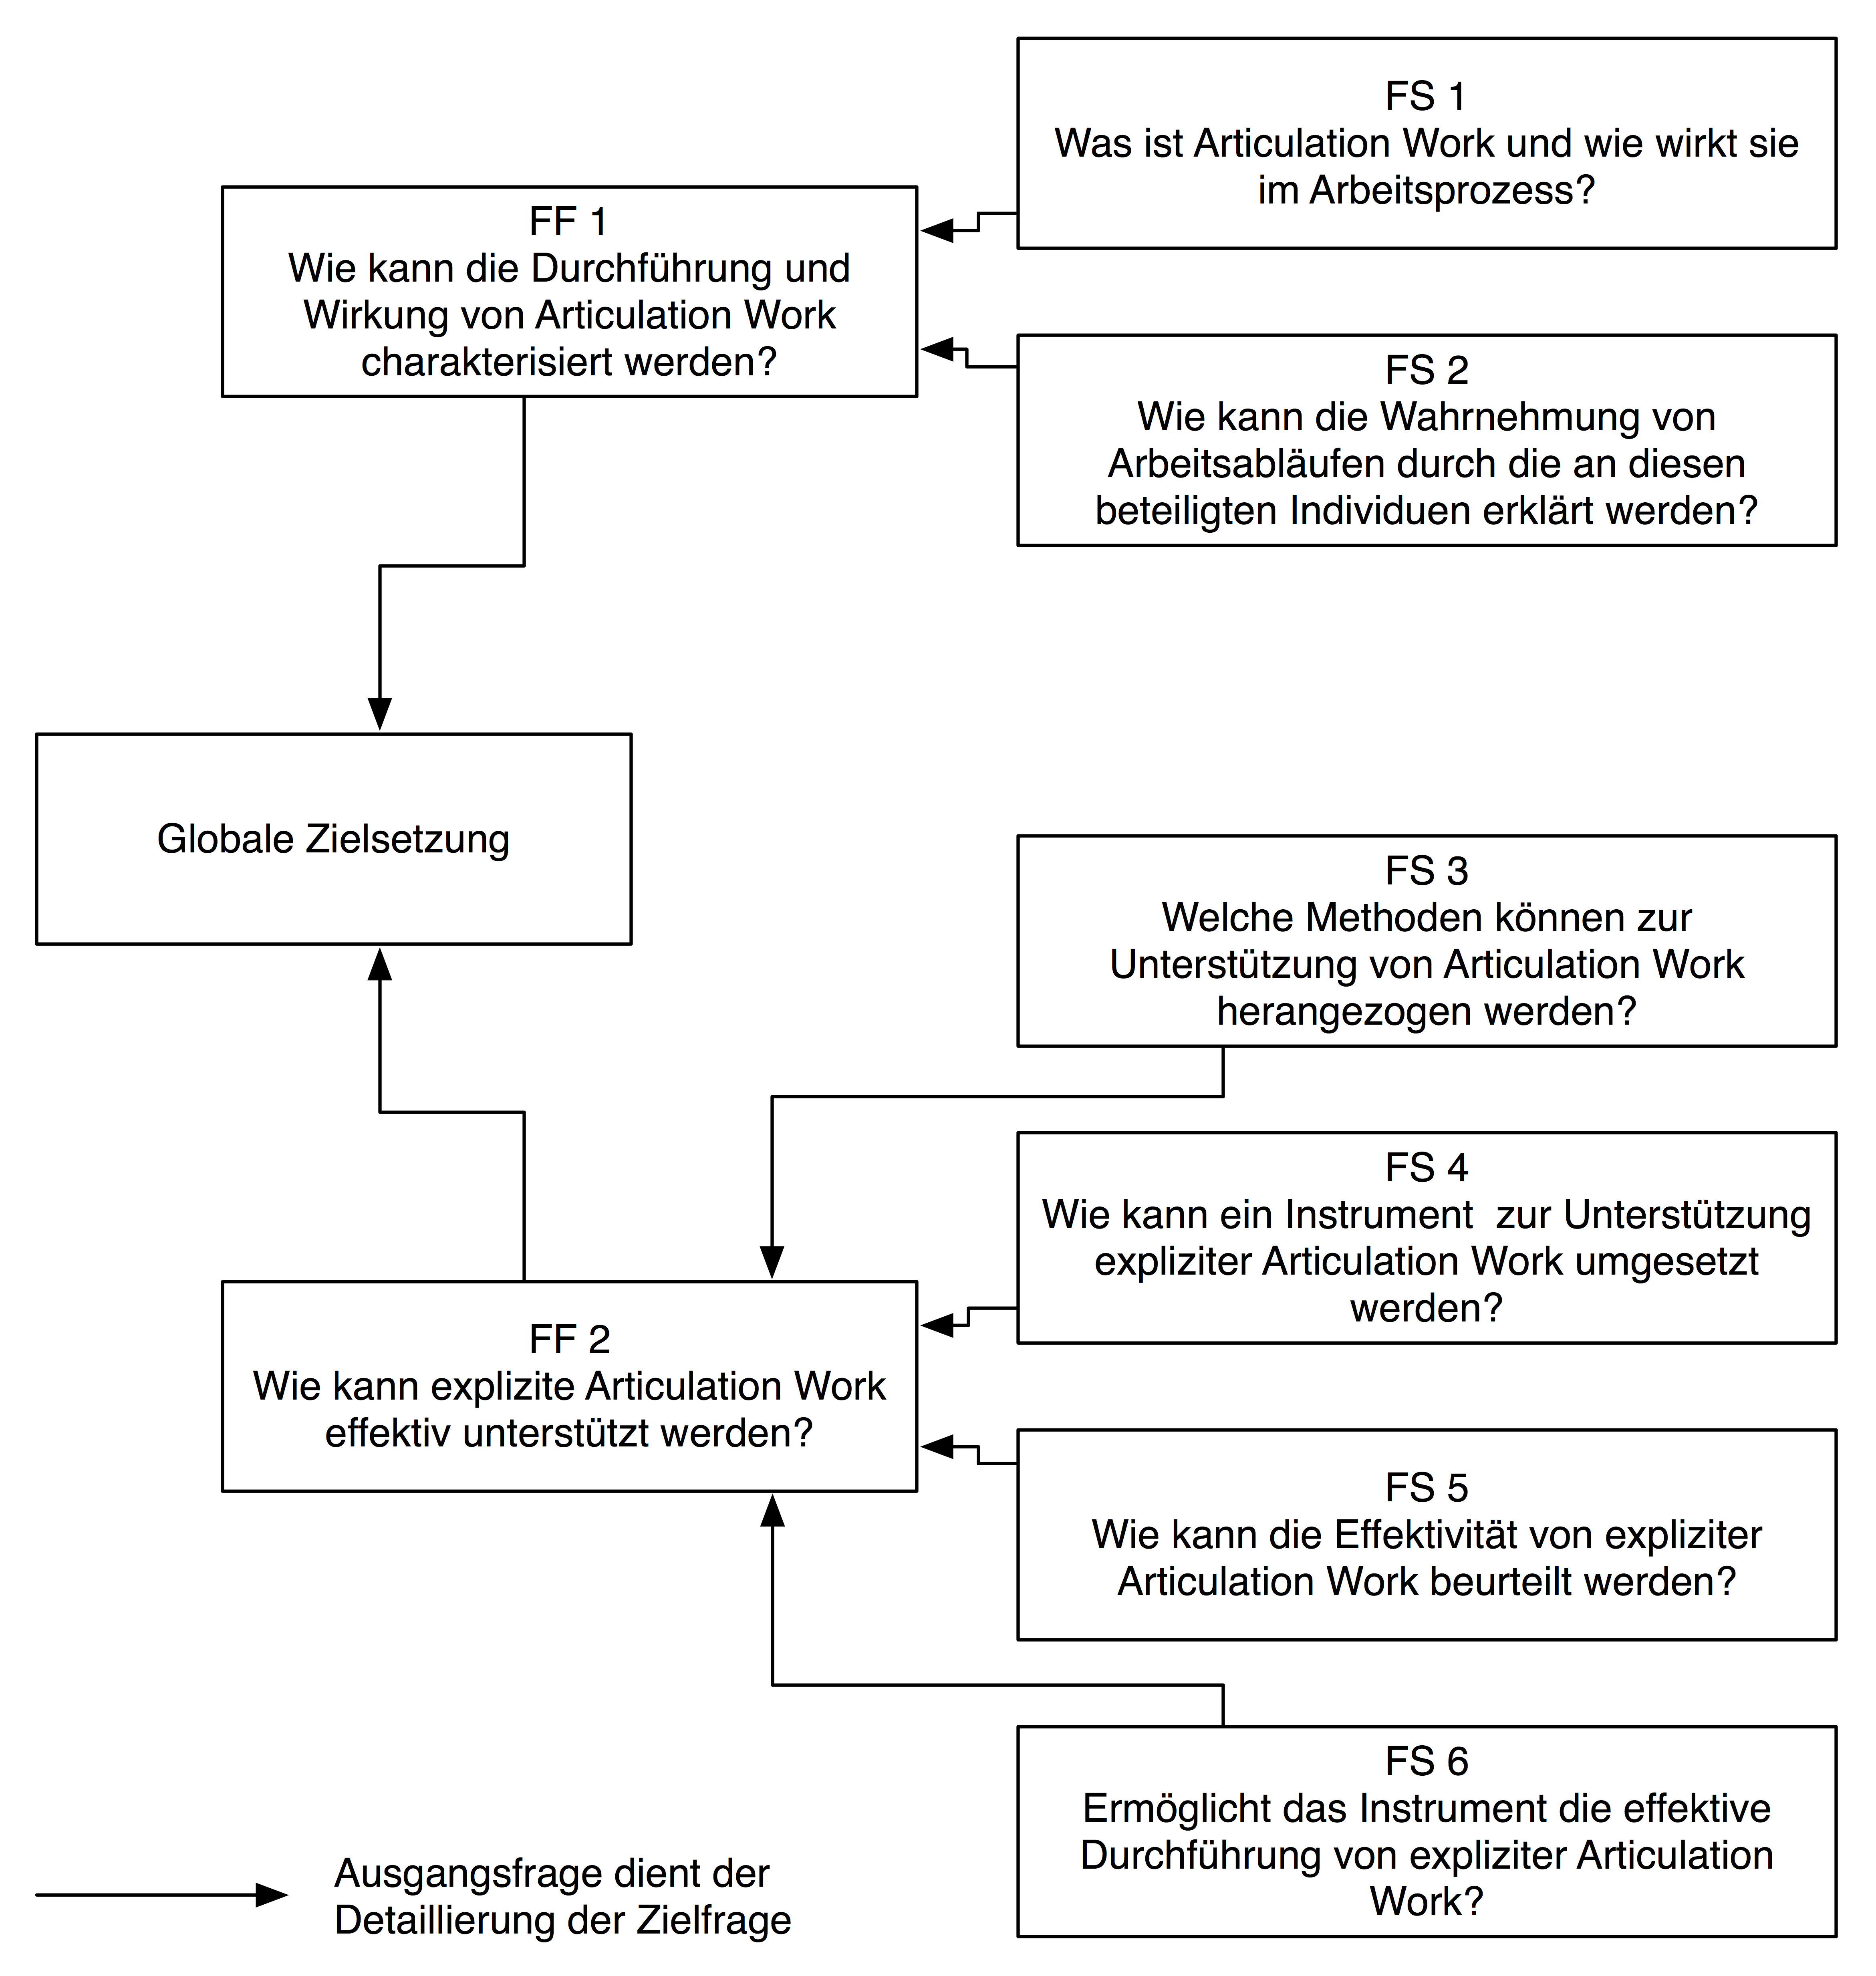
\includegraphics[width=0.9\textwidth]{img/Einfuehrung/zielhierarchie.png}
	\caption{Forschungsfragen und Fragestellungen}
	\label{fig:img_Einfuehrung_zielhierarchie}
\end{figure}

Diese Fragestellungen müssen im Rahmen der Durchführung dieser Arbeit beantwortet werden. Dazu wird in der Zusammenfassung jedes Kapitels auf diese Fragen referenziert und der jeweilige Beitrag zu deren Beantwortung identifiziert. In den Schlussbetrachtungen in Kapitel \ref{cha:schlussbetrachtungen} ist die globale Zielsetzung schließlich wieder aufzugreifen und einer abschließenden Bewertung hinsichtlich ihrer Erfüllung zu unterziehen. 

% section forschungsfragen (end)

% chapter einführung (end)
\section{Aufbau der Arbeit} % (fold)
\label{sec:aufbau_der_arbeit}

In diesem Abschnitt wird die Struktur der Arbeit auf globaler Ebene dargestellt. Zusätzlich wird der inhaltliche Aufbau der einzelnen Kapitel zueinander in Beziehung gesetzt und so der rote Faden durch die Arbeit transparent gemacht.

Die hier vorgestellte Struktur ist auszugsweise auch am Beginn jedes Kapitels beschrieben und graphisch dargestellt, um die Einordnung der Kapitel in den Gesamtzusammenhang der Arbeit zu erleichtern.

\subsection{Überblick} % (fold)
\label{sub:aufbau_ueberblick}

Die Arbeit gliedert sich inhaltlich in drei große Teile, die durch das Einleitungs- und Schlusskapitel eingerahmt werden.

Teil \ref{prt:grundlagen} behandelt die der Unterstützung von „Articulation Work“ zugrunde liegenden Forschungsgebiete und erfasst die in diesen vorgeschlagenen konkreten Maßnahmen und Methoden zur Unterstützung. Der Teil deckt damit die Beantwortung der ersten oben formulierten Forschungsfrage ab und trägt durch die Betrachtung des methodischen Teils der Unterstützung bereits zur Beantwortung der Forschungsfrage 2 bei. Im Einzelnen umfasst Teil \ref{prt:grundlagen} ein Kapitel über „Articulation Work“ (Fragestellung 1, Kapitel \ref{cha:articulation_work}) und ein Kapitel über „Mentale Modelle“ (Fragestellung 2, Kapitel \ref{cha:mentale_modelle}). Teil \ref{prt:grundlagen} endet mit einem Kapitel über Methodik der Anwendungsszenarien, in dem beschrieben wird, wie mentale Modelle für die Verwendung für „Articulation Work“ externalisiert und abgestimmt werden können und trägt damit bereits zur Forschungsfrage 2 bei (Fragestellung 3, Kapitel \ref{cha:methodik}).

Teil \ref{prt:umsetzung} behandelt die Umsetzung des Werkzeugs selbst. Er trägt damit wesentlich zur Beantwortung der zweiten oben formulierten Forschungsfrage bei, indem er das bislang auf methodischer Ebene beschriebene Unterstützungsinstrument technisch vervollständigt. Das erste Kapitel greift die Ergebnisse des ersten Teils auf und leitet daraus die Anforderungen an das Werkzeug ab (Teil der Beantwortung der Fragestellung 4, Kapitel \ref{cha:anforderungen}). In Kapitel \ref{cha:implementierung_Überblick} werden die konzeptuellen Grundlagen für die Implementierung aus dem Kontext von Tangible Interfaces heraus aufgearbeitet. Die Kapitel \ref{cha:input_&_interpretation}, \ref{cha:visualisierung} und \ref{cha:persistierung} beschreiben nacheinander die technische Umsetzung des Werkzeugs -- beginnend von den Eingabekanälen über die Ausgabekanäle bis zu Persistierung der Modelle. Sie beantworten also die Fragestellung 4. 

Teil \ref{prt:evaluierung} behandelt die Evaluierung des Werkzeugs. Er deckt damit im Wesentlichen den zweiten Teil der zweiten Forschungfrage ab, klärt das Konzept der „effektiven Unterstützung von Articulation Work“ und prüft diese für das entwickelt Instument. Dabei beginnt Kapitel \ref{cha:konzeptuelle_evaluierung} mit einer konzeptuellen Betrachtung des umgesetzten Systems (also einer theoretischen Einordnung des Werkzeugs auf Basis der Ergebnisse von Kapitel \ref{cha:implementierung_Überblick}, den konzeptuellen Grundlagen der Implementierung). In Kapitel \ref{cha:eval_ueberblick} werden die grundsätzliche Ausrichtung der empirischen Untersuchung und die durchgeführten Evaluierungen beschrieben. Die Kapitel \ref{cha:eval_werkzeug}, \ref{cha:eval_modell} und \ref{cha:eval_aw} beschäftigen sich mit der Ableitung der Hypothesen und deren Prüfung auf den unterschiedlichen Untersuchungsebenen der Arbeit. Dies beginnt mit der Prüfung der grundsätzlichen Verwendbarkeit des Systems (Kapitel \ref{cha:eval_werkzeug}), setzt mit der Prüfung der Eignung für die Externalisierung mentaler Modelle fort (Kapitel \ref{cha:eval_modell}) und endet mit der Prüfung der Eignung für „Articulation Work“ selbst (Kapitel \ref{cha:eval_aw}).

In der Zusammenfassung jedes Kapitels wird auf die betroffenen Fragestellung referenziert und der jeweilige Beitrag zur Erreichung der globalen Zielsetzung identifiziert. Der Schlussteil (Kapitel \ref{cha:schlussbetrachtungen}) fasst die Ergebnisse der Arbeit nochmals zusammen und spiegelt diese in ihrer Gesamtheit auf die ursprüngliche Zielsetzung zurück.

Die Gesamtstruktur dieser Arbeit ist in Abbildung \ref{fig:img_Einfuehrung_gesamtueberblick} nochmals zusammenfassend dargestellt. Die Beziehungen zwischen den einzelnen Kapiteln sind als Pfeile zwischen den einzelnen Blöcken dargestellt, wobei jeweils der Endpunkt Ergebnisse des Startpunktes als Grundlage für die weiteren Ausführungen verwendet.

\begin{figure}[htbp]
	\centering
		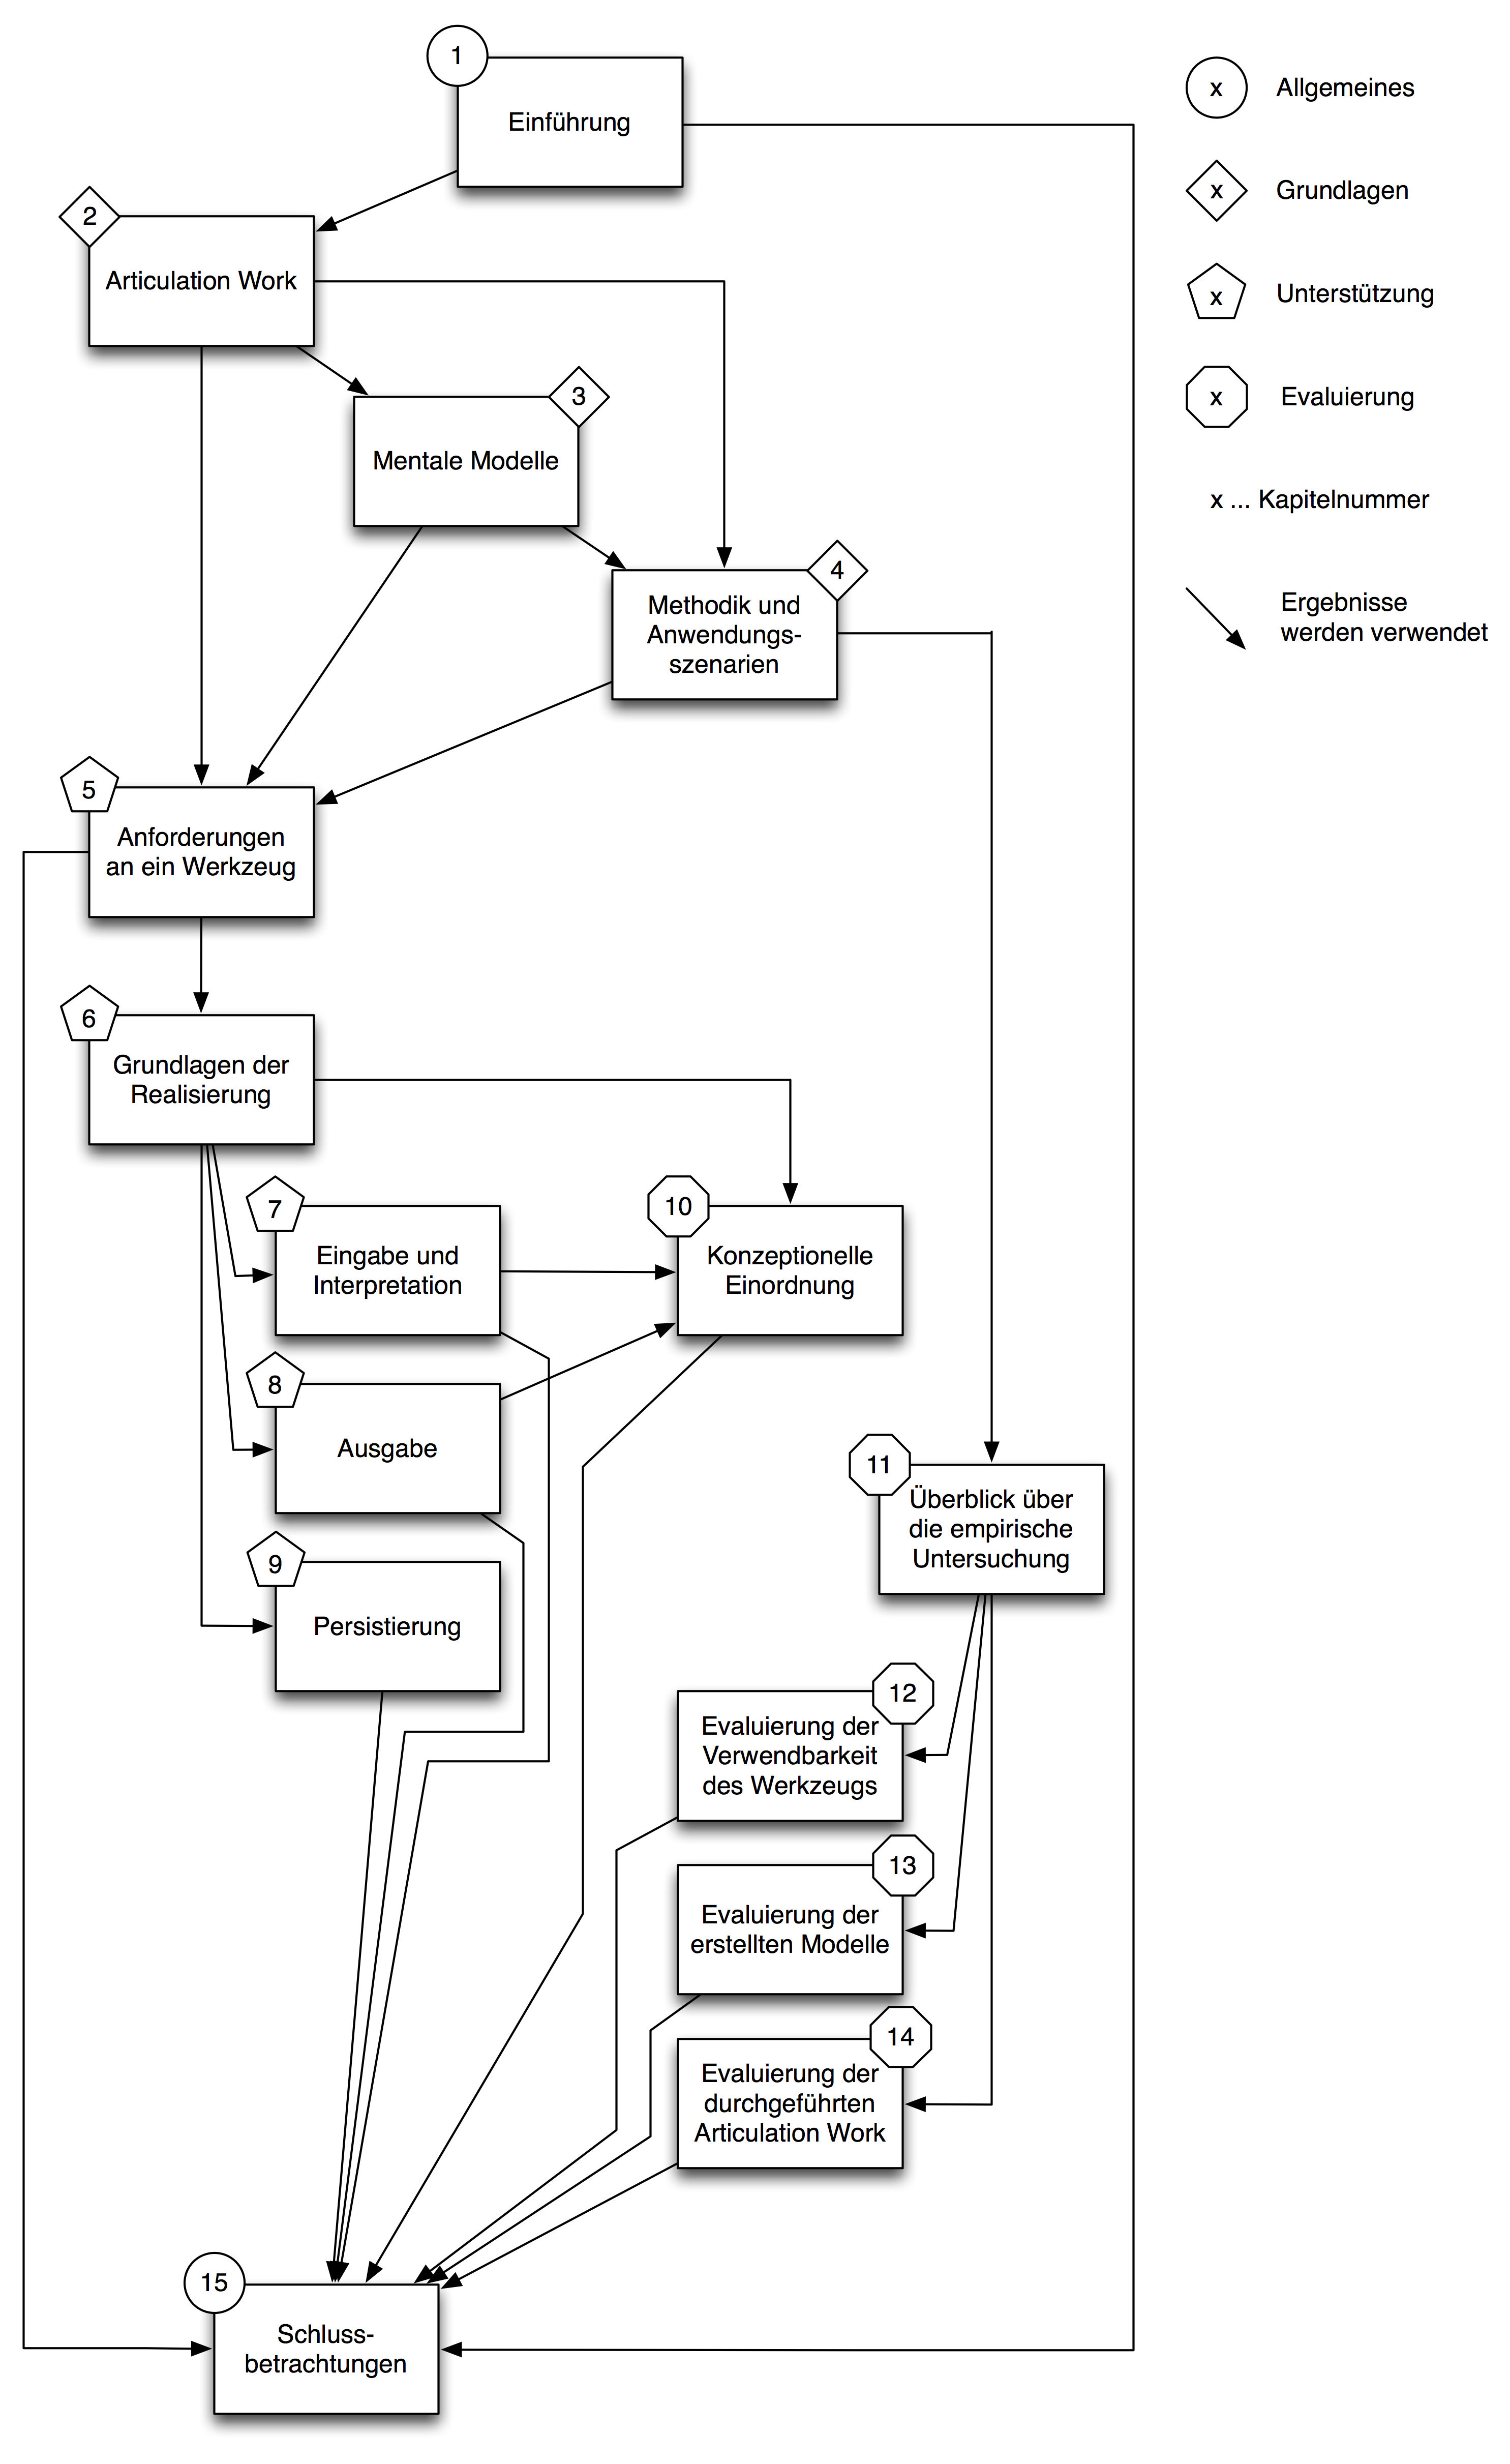
\includegraphics[height=0.9\textheight]{img/Einfuehrung/gesamtueberblick.png}
	\caption{Zusammenhänge zwischen den Kapiteln der Arbeit}
	\label{fig:img_Einfuehrung_gesamtueberblick}
\end{figure}

Anhang \ref{cha:literatur_zum_themengebiet_articulation_work} ist als Ergänzung zu Kapitel \ref{cha:articulation_work} (Articulation Work) zu sehen und stellt die gesamte zu diesem Gebiet erschienene Literatur strukturiert dar.

Anhang \ref{cha:daten_der_empirischen_untersuchung} ergänzt die Evaluierungskapitel in Teil \ref{prt:evaluierung} durch eine Zusammenfassung der im Rahmen der Untersuchung erhobenen Daten.
% subsection aufbau_ueberblick (end)

\subsection{Zusammenfassung der Zusammenhänge} % (fold)
\label{sub:zusammenhänge}

Dieser Abschnitt stellt die wesentlichen inhaltlichen Zusammenhänge der Arbeit dar und vermittelt so ein erstes Bild des roten Fadens durch die Arbeit. Er ergänzt somit die im letzten Abschnitt dargestellte Struktur der Arbeit um eine detaillierte inhaltliche Sicht und fasst das Vorgehen bei der Bearbeitung der in Abschnitt \ref{sec:forschungsfragen} formulierten Forschungsfragen zusammen.

Kapitel \ref{cha:articulation_work} beginnt mit einer generellen Begriffsbestimmung zum Themenfeld „Articulation Work“. Diese bildet die Grundlage für den nächsten Abschnitt, in dem auf Basis der Literatur geklärt wird, wie sich „Articulation Work“ manifestiert und in welchen unterschiedlichen Ausprägungen sie das tut. Das Ergebnis ist in Abbildung \ref{fig:img_ArticulationWork_aw_conceptual_structure} zusammengefasst und spannt die in dieser Arbeit verwendete Taxonomie auf. In den beiden folgenden Abschnitten wird auf Basis der Literatur dargestellt, was (welche Arbeitsaspekte) Gegenstand von „Articulation Work“ ist und wie „Articulation Work“ unterstützt werden kann (siehe dazu auch Anhang \ref{cha:literatur_zum_themengebiet_articulation_work} für eine Gesamtübersicht über die zu „Articulation Work“ verfügbare Literatur). Schließlich greift der letzte Abschnitt die Ergebnisse der Literaturstudien wieder auf und identifiziert eine konzeptuelle Lücke bei der Betrachtung von kooperativer Arbeit anhand der Theorie von Strauss, die auch schon im Rahmen der Einleitung identifiziert wurde  -- nämlich die bislang vernachlässigte Rolle des Individuums bei „Articulation Work“ und dessen konkrete Tätigkeiten. Zu diesem Aspekt existieren wenige Aussagen in der Literatur zu „Articulation Work“, \citet{Strauss93} selbst weist jedoch darauf hin, dass eine konzeptuelle Lücke entsteht, wenn auf die sozialen und organisationalen Aspekte von „Articulation Work“ fokussiert wird, die individuellen „thought processes“ aber außer Acht gelassen werden.

In Kapitel \ref{cha:mentale_modelle} wird die identifizierte Lücke aufgegriffen und konzeptuell mit dem Erklärungsmodell der mentalen Modelle \citep{Johnson-Laird81} hinterlegt. Im Kontext von „Articulation Work“ sind mentale Modelle jener Beitrag, den jedes beteiligte Individuum einbringt und der in der Folge Gegenstand der Abstimmung und Aushandlung sein muss, um eine gemeinsame Sichtweise zu entwickeln und „contingencies“ aufzulösen (was letztendlich das Ziel von „Articulation Work“ ist \citep{Gerson86}). Dementsprechend beschäftigt sich der nächste Abschnitt mit der Bildung und Veränderung mentaler Modelle, wobei als wesentliches Hilfsmittel dazu die Externalisierung derselben identifiziert wird \citep{Seel91}. Zur Externalisierung werden drei in der Literatur genannte Ansätze vorgestellt \citep{Ifenthaler06}. Diesen sind Strukturlegetechniken \citep{Dann92} sowie Concept Mapping \citep{Novak06} zuzurechnen, die in der Folge durch ihre kooperative Anwendbarkeit als die für „Articulation Work“ am besten geeigneten Ansätze identifiziert werden (vor allem Strukturlegetechniken unterstützen inhärent den Abstimmungsprozess von mentalen Modellen \citep{Groeben00}).

Dies führt zu Kapitel \ref{cha:methodik}, in dem auf Basis der beiden Ansätze die Methoden zur Externalisierung von mentalen Modellen beschrieben werde. Diese werden den Eigenschaften von „Articulation Work“ gegenüber gestellt und daraus ein Vorgehen abgeleitet, dass Strukturlegetechniken und Concept Mapping in einer Methodik zusammenführt. Diese Methodik soll möglichst offen (im Sinne von prozedural und inhaltlich flexibel) die Externalisierung und Abstimmung mentaler Modelle ermöglichen. Der zweite Teil des Kapitels stellt mögliche Anwendungsszenarien vor, die im Kontext von „Articulation Work“ auftreten können. Diese Anwendungsszenarien schlagen die Brücke zu den Anwendungen im Rahmen der Evaluierung (siehe Kapitel \ref{cha:eval_ueberblick}), da diese den einzelnen Evaluierungsteilen zugeordnet werden können.

Das Methodik-Kapitel leitet in Teil \ref{prt:umsetzung} der Arbeit über, wo die konkrete Unterstützung von „Articulation Work“ durch ein Werkzeug besprochen wird. Als Ausgangspunkt für das Kapitel \ref{cha:anforderungen} wird auf Teil \ref{prt:grundlagen} und dort speziell auf das Kapitel zur Methodik zurückgegriffen und aus den dortigen Ergebnissen Anforderungen an ein Werkzeug abgeleitet, das die vorgeschlagene Vorgehensweise unterstützt. Konzeptuell ist hier zwischen Anforderungen zu unterscheiden, die aus der Concept Mapping Methodik stammen (im Wesentlichen „Flexibilität der Repräsentation“), Anforderungen, die von Strukturlegetechniken abzuleiten sind (im Wesentlichen „Physikalität der Repräsentation“) und jenen, die direkt aus „Articulation Work“ abgeleitet werden können (im Wesentlichen „Kooperative Bedienbarkeit“).

Die Festlegung dieser Anforderungen ist die Grundlage der konkreten Umsetzung des Werkzeugs. Kapitel \ref{cha:anforderungen} endet mit der Feststellung, dass aufgrund der Anforderungen aus allen drei Bereichen ein „Tangible Tabletop Interface“ geeignet wäre, entsprechende Werkzeugunterstützung zu liefern. „Tangible“ motiviert sich dabei aus der in Strukturlegetechniken geforderten Physikalität der Abbildung, „Tabletop“ aus der unmittelbaren kooperativen Bearbeitbarkeit, die durch „Articulation Work“ selbst gefordert wird und „Interface“ (in diesem Kontext ist darunter die Rechnerunterstützung zu verstehen) durch die im Rahmen von Concept Mapping vorgeschlagenen Maßnahmen zur Modellierungsunterstützung, die nur durch Funktionen im Rechner realisiert werden können.

Vor der konkreten Umsetzung geht das folgende Kapitel (Kapitel \ref{cha:implementierung_Überblick}) detailliert auf die Thematik der „Tangible Tabletop Interfaces“ ein. Neben einem historischen Überblick schlägt Abschnitt \ref{sec:lernprozesse_und_tangible_interface} ausgehend von der eher technologiezentrierten Sichtweise der „Tangible Interface“-Forschung die Brücke zurück zu den mentalen Modellen und Lernprozessen, die in Kapitel \ref{cha:mentale_modelle} („Mentale Modelle“) besprochen wurden. Einige der genannten Aspekte lassen sich auch auf die Anforderungen von „Articulation Work“ abbilden, was im zweiten Teil dieses Abschnitts beschrieben wird. Als zweiten Brückenschlags in den Grundlagenteil wird die Forschung zu den Auswirkungen von „Tangible Interfaces“ auf die Kooperation der Anwender betrachtet -- ein Bereich der unmittelbar für „Articulation Work“ selbst relevant ist und damit die Brücke zurück zu Kapitel \ref{cha:articulation_work} schlägt. Mit diesen beiden Abschnitten (\ref{sec:lernprozesse_und_tangible_interface} und \ref{sec:kooperation_und_tangible_interfaces}) wird nochmals (aus „technischer“ Sicht) begründet, das „Tangible Interfaces“ für den geplanten Anwendungsbereich (kooperative Externalisierung und Abstimmung mentaler Modelle) geeignet sind.

Der zweite Teil von Kapitel \ref{cha:implementierung_Überblick} (ab Abschnitt \ref{sec:konzeptualisierungen_von_tangible_interfaces}) beschäftigt sich mit Ansätzen, „Tangible Interfaces“ konzeptuell zu betrachten. Dazu wird die existierende Literatur umfassend aufgearbeitet und strukturiert dargestellt. Dieser Teil wird in Kapitel \ref{cha:konzeptuelle_evaluierung} wieder aufgegriffen und zur Einordnung des entwickelten Systems in den Designraum der „Tangible Interface“-Forschung verwendet. Auch in den Kapiteln \ref{cha:input_&_interpretation} und \ref{cha:visualisierung}, die die konkrete Umsetzung des Werkzeugs beschreiben, wird auf einzelne dieser konzeptuellen Erklärungsmodelle zurückgegriffen, die explizit für die Unterstützung der Konzeption von Tangible Interfaces entwickelt wurden.

Teil 3 von Kapitel \ref{cha:implementierung_Überblick} wird wieder konkreter und engt den Betrachtungsbereich von „Tangible Interfaces“ auf „Tabletop Interfaces“ ein, um letztendlich auf „Tabletop Interfaces zur Erstellung diagrammatischer Modelle“ zu fokussieren, was im Wesentlichen die unmittelbare „Related Work“ zu der vorliegenden Arbeit aus technischer Sicht darstellt. Auch dazu wird jeweils die verfügbare Literatur (aus historischer Sicht sowie den „State of the Art“) aufgearbeitet.

Nach diesem umfassenden Überblickskapitel behandeln die Folgekapitel die konkrete technische Umsetzung des Werkzeugs. Das Werkzeug wurde dazu konzeptuell in drei Blöcke unterteilt. Kapitel \ref{cha:input_&_interpretation} beschäftigt sich mit der Eingabe von Information über das „Tabletop Interface“ und der Aufbereitung und Interpretation der Eingabedaten für den spezifischen Anwendungsfall (also der „Modellierung“). Dabei erfolgt die Beschreibung vom Allgemeinen ins Spezielle und beginnt mit der Darstellung der grundlegenden Möglichkeiten, auf einem „Tabletop Interface“ Benutzereingaben zu ermöglichen. Auf Basis der Anforderungen aus Kapitel \ref{cha:anforderungen} wird eine Technologieentscheidung getroffen (optische Erkennung der Bausteine). Dazu werden in der Folge die in diesem Bereich verfügbaren Softwareframeworks dargestellt und wiederum strukturiert gegenübergestellt. Die folgende Framework-Entscheidung für das ReacTIVision-System \citep{Kaltenbrunner07} ermöglicht die Festlegung des konkrete Hard- und Softwaredesign für die Erkennung von Benutzereingaben. In den folgenden Abschnitten wird die Implementierung beginnend von der Benutzungsschnittstelle (in diesem Fall Hardware) hin zur Richtung Software zur Erkennung und Interpretation der Benutzereingaben dargestellt. Nach der Beschreibung der Hardware in Abschnitt \ref{sec:konzeption_und_umsetzung_der_hardwarekomponenten} wird in Abschnitt \ref{sec:benutzerinteraktion_mit_dem_werkzeug} die Interaktion der Benutzer mit dem Werkzeug beschrieben. Damit kommt die Anwendungssicht (also die „Modellierung“) ins Spiel, die benötigt wird, um die Interpretation der Eingabedaten zu beschreiben. Dies erfolgt in Abschnitt \ref{sec:erfassung_der_benutzerinteraktion_durch_softfware}. Das Kapitel endet an jenem Punkt, wo auch in der Software eine Schnittstelle zur Entkopplung und Modularisierung eingeführt wurde -- bei der Übergabe der interpretierten und auf Modellierungsaktivitäten abstrahierten Eingabedaten an die weiterverarbeitenden Schichten (siehe Abbildung \ref{fig:img_ImplementierungInput_InputArchitecture}).

Kapitel \ref{cha:visualisierung} widmet sich der Ausgabe und ist analog zu Kapitel \ref{cha:input_&_interpretation} aufgebaut. Beginnend von den grundsätzlichen Möglichkeiten zur Ausgabe immer weiter fokussiert, bis die konkreten Umsetzung der Informationsausgabe mittels dem JHotDraw-Framework \citep{Gamma96} dargestellt werden kann. Wo in Kapitel \ref{cha:input_&_interpretation} durch Beschreibung der Benutzerinteraktionen auf den konkreten Anwendungsfall der Technologie fokussiert wurde, wird hier zum gleichen Zweck die Beschreibung und Zuordnung der auszugebenden Information in Abschnitt \ref{sec:ausgabe_von_information} beschrieben und die Unterscheidung getroffen, ob die Ausgabe direkt auf der Tischoberfläche oder disloziert auf einer separaten Darstellungsfläche zu passieren hat. Die Feststellung, dass mehrere Ausgabekanäle benötigt werden, um die auszugebende Information darstellen zu können, führt zum konkreten Softwaredesign in Abschnitt \ref{sec:umsetzung_der_ausgabe_mit_software}. Dieses ist durch den Einsatz eines Dispatchers modular aufgebaut und erweiterbar angelegt (siehe Abbildung \ref{fig:img_ImplementierungOutput_OutputArchitecture} bzw. Abbildung \ref{fig:img_ImplementierungOutput_OutputClasses}).

In Kapitel \ref{cha:persistierung} wird die Persistierung der erstellten Modelle und der gewonnenen Metainformation besprochen. Dazu identifiziert der einleitende Abschnitt auf Basis der Notwendigkeit einer flexiblen Repräsentationsform „Topic Maps“ \citep{TMDM08} als ein geeignetes Mittel für die Abbildung. In der Folge wird  wieder auf den konkreten Anwendungsfall eingegangen. Nach der Beschreibung von „Topic Maps“ wird die Abbildung der erstellten Modelle auf „Topic Maps“ und letztendlich die konkrete Implementierung der Persistierung dargestellt. Abschnitt \ref{sec:export_graphischer_repräsentationen} stellt die unterschiedlichen Möglichkeiten zum graphischen Export der Modelle dar, der für die unmittelbare Dokumentation des Modellierungsprozesses und -ergebnisses notwendig ist. Dieses Kapitel schließt Teil \ref{prt:umsetzung} der Arbeit ab.

In Teil \ref{prt:evaluierung} wird die Evaluierung des Werkzeugs behandelt. Dies beginnt mit der konzeptuellen Einordnung des erstellten Werkzeugs. Dazu werden sämtliche Ansätze zur Konzeptualisierung von Tangible Interfaces aus Abschnitt \ref{sec:konzeptualisierungen_von_tangible_interfaces} herangezogen und das Werkzeug in seiner aktuellen Implementierung in diese eingeordnet. Das Ziel ist dabei einerseits, das Werkzeug in die bisherige Forschung einzuordnen, andererseits aber auch etwaiges Verbesserungspotential zu identifizieren, das etwa durch Inkonsistenzen der Ausprägungen innerhalb der jeweiligen Betrachtungsdimensionen aufgedeckt werden kann. Während die Einordnung in allen 12 betrachteten Ansätzen möglich ist, kann Verbesserungspotential nur in 7 Ansätzen identifiziert werden. In der Zusammenfassung des Kapitels wird einerseits die Eignung eines Ansatzes zur Einordnung des vorliegenden Systems und der ggf. entstehenden Mehrwert besprochen. Andererseits wird das Verbesserungspotential aufgezeigt, das sich aus der rein konzeptuellen Betrachtung des Systems ableiten lässt. Im Rahmen der empirischen Untersuchung in den folgenden Kapiteln werden diese Punkte aufgegriffen und hinsichtlich ihrer tatsächlich in der Praxis aufgetretenen Relevanz betrachtet.

Die Kapitel \ref{cha:eval_ueberblick} bis \ref{cha:eval_aw} beschreiben die empirische Untersuchung. Kapitel \ref{cha:eval_ueberblick} ist dabei wiederum als Übersichtskapitel konzipiert. Dort werden die zu untersuchenden Aspekte aus der Zielsetzung abgeleitet und die Einteilung in die Kapitel \ref{cha:eval_werkzeug} bis \ref{cha:eval_aw} argumentiert. Untersuchungen werden auf Ebene des Werkzeugs (Benutzbarkeit), der „Mentalen Modelle“ (Eignung des Werkzeugs zur Externalisierung) sowie von „Articulation Work“ selbst (Unterstützung des Aushandlungsprozesses) durchgeführt. Für jeden dieser Blöcke wird eingeführt, auf Basis welcher Literatur die Untersuchung angelegt werden kann. In der darauf folgenden Beschreibung des globalen Untersuchungsdesigns werden alle durchgeführten Untersuchungen vorgestellt. Diese Vorstellung umfasst den Anwendungskontext, die Aufgabenstellung sowie die Beschreibung der Teilnehmer bzw. deren Hintergrund. Die Zuordnung zwischen den Untersuchungen und den untersuchten Aspekten erfolgt im Rahmen der Vorstellung der jeweiligen Untersuchung und zusammengefasst nochmals im letzen Abschnitt des Kapitels. Nach der Vorstellung der Untersuchungen werden die eingesetzten empirischen und statistischen Methoden beschrieben, auf die in den Kapiteln \ref{cha:eval_werkzeug} bis \ref{cha:eval_aw} nur noch namentlich verwiesen wird.

Die Kapitel \ref{cha:eval_werkzeug} bis \ref{cha:eval_aw} widmen sich der Prüfung der drei identifizierten Untersuchungsebenen. Alle drei Kapitel sind identisch aufgebaut. Im jeweils ersten Abschnitt werden die zu prüfenden Hypothesen abgeleitet. Diese Ableitung erfolgt aus der Zielsetzung, hinterlegt mit den konzeptuellen Grundlagen der Arbeit aus Teil \ref{prt:grundlagen}. Zusätzlich werden explorativ gebildete Hypothesen formuliert, die nicht unmittelbar aus der Zielsetzung ableitbar sind, die aber Auffälligkeiten abbilden, die im Rahmen der ersten, explorativen Untersuchungen des Werkzeugs offensichtlich wurden und die an dieser Stelle nochmals dezidiert geprüft werden sollen, um die Vermutungen zu bestätigen oder diese  widerlegen zu können. Im auf die Formulierung der Hypothesen folgenden Abschnitt über Untersuchungsdesign und Durchführung werden einerseits die Hypothesen operationalisiert (d.h. deren konkrete Prüfung vorgestellt und argumentiert) und in der Folge die Durchführung der Untersuchungen beschrieben. An dieser Stelle wird auf die im vorhergehenden Kapitel vorgestellten Untersuchungen zurückgegriffen und der jeweils relevante Teil im Detail beschrieben. Der dritte Abschnitt jedes Kapitels präsentiert die Ergebnisse der Untersuchung. Für jede Hypothese wird die Auswertung durchgeführt, das Ergebnis diskutiert und in einem separaten Unterabschnitt nochmals zusammengefasst. Die Beschreibung der Auswertung umfasst dabei sowohl quantitative Daten (z.T. graphisch aufbereitet) als auch qualitative Ergebnisse, die meist in der Form von Transkripten von Auszügen aus Modellierungsprozessen eingefügt werden.

In den Schlussbetrachtungen in Kapitel \ref{cha:schlussbetrachtungen} werden die Ergebnisse der Evaluierung zusammengefasst und auf Anforderungen an das Werkzeug sowie die globale Zielsetzung rückgespiegelt. Aufbauend darauf werden weitere Entwicklungsmöglichkeiten des Werkzeugs aufgezeigt und weiterführende Anwendungsszenarien beschrieben. Eine Reflexion des gesamten Entstehungsprozesses schließt diese Arbeit ab.

Abbildung \ref{fig:img_Einfuehrung_zusammenhang} stellt die Bezüge zwischen den Kapitel und den zu bearbeitenden Fragestellungen nochmals graphisch dar. Die hier abgebildeten Bezüge werden auch in den Zusammenfassungen der jeweiligen Kapitel beschrieben und inhaltlich argumentiert.

\begin{figure}[htbp]
	\centering
		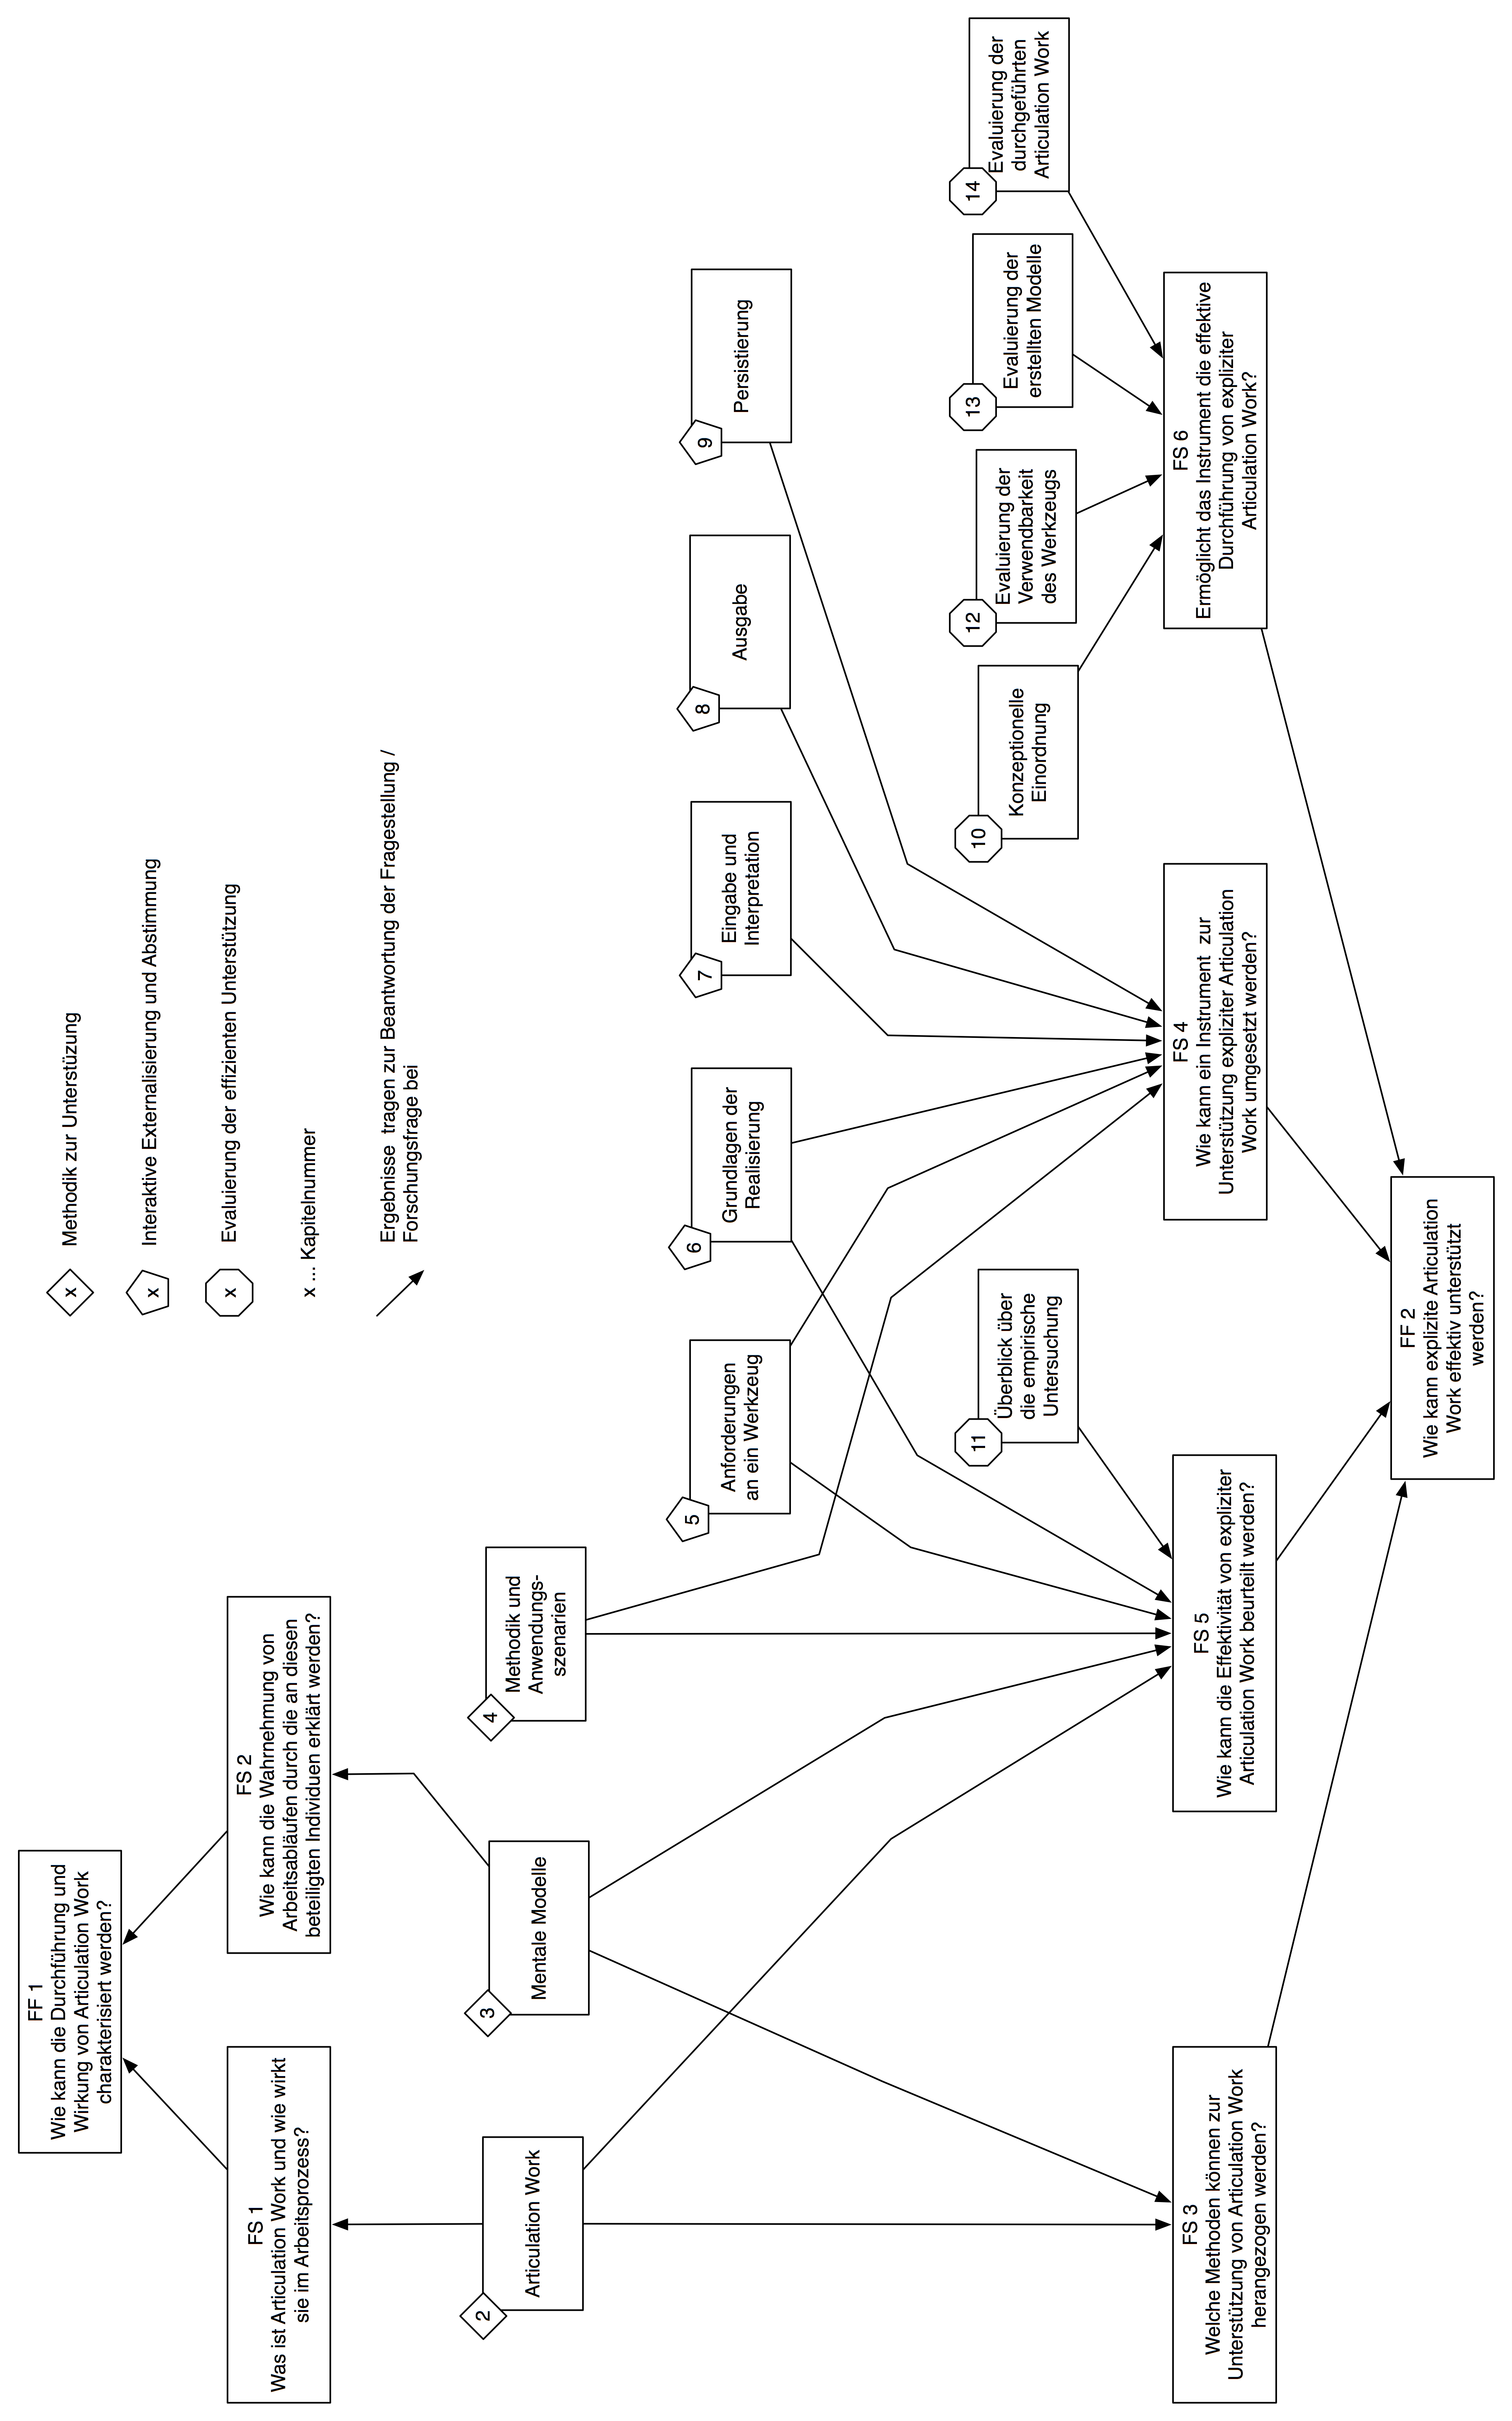
\includegraphics[height=.9\textheight]{img/Einfuehrung/zusammenhang.png}
	\caption{Zusammenhang zwischen Zielsetzung und Struktur der Arbeit }
	\label{fig:img_Einfuehrung_zusammenhang}
\end{figure}


% subsection zusammenhänge (end)
% section aufbau_der_arbeit (end)


\part{Grundlagen} % (fold)
\label{prt:grundlagen}

\section*{Einleitung} % (fold)
\label{sec:grundlagen_einleitung}
\thispagestyle{empty}

Dieser Teil stellt die dieser Arbeit zugrundeliegenden Konzepte und deren Auswirkungen auf die Erreichung der globalen Zielsetzung vor. Ziel dieses Teil ist es, diese Konzepte umfassend darzulegen und in der existierenden Literatur Möglichkeiten bzw. Ansatzpunkte zur Unterstützung expliziter Articulation Work zu identifizieren.

Wie bereits in Kapitel \ref{cha:einführung} beschrieben, 

AW motivieren

Mentale Modelle motivieren

Externalisierung motivieren

Aufbau des Teils beschreiben

% section grundlagen_einleitung (end)

\chapter{Articulation Work} % (fold)
\label{cha:articulation_work}

In diesem Kapitel wird das Konzept „Articulation Work“ dargestellt und in den Kontext von menschlicher Arbeit an sich gestellt. Der zweite Teil des Kapitels widmet sich den Aktivitäten, die „Articulation Work“ ausmachen, den Merkmalen, an denen sich gute „Articulation Work“ zeigt, sowie den Möglichkeiten der Unterstützung von „Articulation Work“ durch organisationale und technische Maßnahmen.

\section{Begriffsbestimmung} % (fold)
\label{sec:aw_begriffsbestimmung}

Das Konzept der "Articulation Work" wurde als Erklärungsmodell für einen bestimmten Typus von menschlicher Arbeit Mitte der 1980er Jahre von  \citet{Strauss85} im Kontext von Fallstudien aus der Krankenhaus-Organisation eingeführt. "Articulation Work" ist dabei jener Anteil an menschlicher Arbeit, der der Abstimmung mit anderen Individuen dient. Diese Abstimmung ist notwendig um das eigentliche Arbeitsziel erreichen zu können. Arbeit wird als inhärent kooperative Prozess gesehen, der immer auf Interaktion mit anderen Menschen basiert bzw. diese bedingt (Strauss formuliert diese Annahme in Bezugnahme auf \citet{Hughes71} prägnant mit der Aussage \emph{„work rests ultimately on interaction“}). Diese Annahme erscheint insofern als zulässig, als dass selbst Arbeitsabläufe, die selbst keine Kooperation mit anderen Menschen bedingen, zumindest auf den Ergebnissen anderer Arbeitsabläufe aufbauen oder als Grundlage weiterer Arbeitsabläufe dienen. Interaktion tritt also in jedem Arbeitsprozess zumindest zu Beginn und am Ende in unmittelbarer oder mittelbarer\footnote{Unter "mittelbar" ist hier Interaktion zu verstehen, die nicht im direkten Kontakt zwischen Individuen abläuft sondern lediglich indirekt durch die Ergebnisse eines Arbeitsprozesses (Materialien, Dokumente, \ldots) vermittelt wird.} Form auf.

\textbf{Abbildung, in der kooperative Arbeitsprozesse und solche mit mittelbarer und unmittelbarer Interaktion zu Beginn oder am Ende dargestellt werden}

Jener Teil von Arbeit, der der eigentlichen Zielerreichung dient, wird im hier vorgestellten Erklärungsmodell als „Production Work“ bezeichnet \citep{Fujimura87}. „Production Work“ ist komplementär zu „Articulation Work“ zu sehen und umfasst alle Aktivitäten, die der „Wertschöpfung“ im wörtlichen Sinn, also der Schaffung jener Werte (oder Ergebnisse), die durch den Arbeitsablauf erreicht werden sollten. Wenn hier von Arbeit bzw. Arbeitsabläufen die Rede ist, so ist darunter eine Kette von Aktivitäten zu verstehen, die der Erreichung eine vorab gewählten Ziels dient\footnote{siehe dazu etwa die Definition von Arbeit durch \citet{Semmer04}: \emph{„Arbeit ist zielgerichtete menschliche Tätigkeit zum Zwecke der Transformation und Aneignung der Umwelt aufgrund selbst- oder fremddefinierter Aufgaben, mit gesellschaftlicher, materieller oder ideeller Bewertung, zur Realisierung oder Weiterentwicklung individueller oder kollektiver Bedürfnisse, Ansprüche und Kompetenzen.“}}. 

\begin{figure}[htbp]
	\centering
		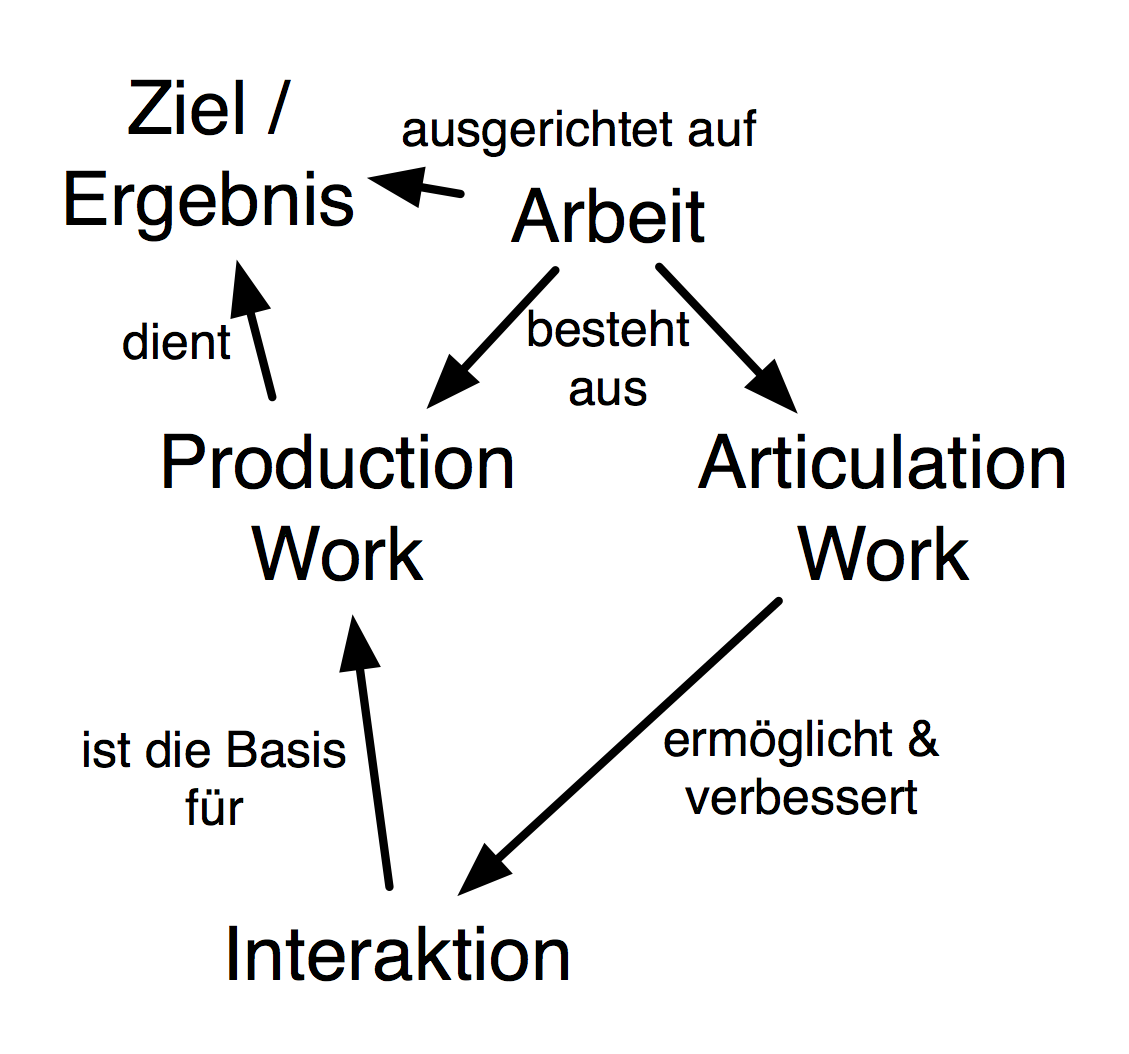
\includegraphics[height=3in]{img/ArticulationWork/ArbeitInteraktion.png}
	\caption{Struktur von Arbeitsabläufen}
	\label{fig:img_ArticulationWork_ArbeitInteraktion}
\end{figure}

Teile eines Arbeitsablaufs dienen also der Zielerreichung an sich („Production Work“). Andere Teile dienen der Abstimmung zwischen den involvierten Akteuren, um ein gemeinsames Verständnis über die jeweiligen Schnittstellen – also die Berührungspunkte zwischen den Tätigkeiten – zu entwickeln. Diese „Koordination“ ist kritisch für den Erfolg von kooperativer Arbeit \citep{Strauss93} und wird als „Articulation Work“ bezeichnet.\footnote{\emph{„Without an understanding of articulation, the gap between requirements and the actual work process in the office will remain inaccessible to analysis. That is, it will be possible to describe tasks in an idealized form but not to describe actual situations.“}\citep{Gerson86}} „Articulation Work“ ist damit ein Enabler für funktionierende Kommunikation und Koordination im eigentlichen Arbeitsprozess\footnote{\emph{"Reconciling incommensurate assumptions and procedures in the absence of enforceable standards is the essence of articulation. Articulation consists of all the tasks involved in assembling, scheduling, monitoring, and coordinating all of the steps necessary to complete a production task."}\citep{Gerson86}}. 

\begin{figure}[htbp]
	\centering
		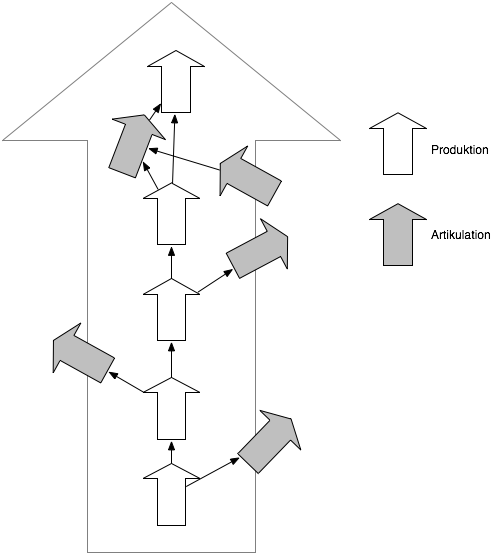
\includegraphics[height=3in]{img/ArticulationWork/ArtikulationProduktion.png}
	\caption{Konzeptualisierung von „Arbeit“ nach \citep{Strauss85} und \citep{Fujimura87}}
	\label{fig:img_ArticulationWork_ArtikulationProduktion}
\end{figure}

Der Begriff „Articulation Work“ ist im Englischen zweideutig und von Strauss bewusst so gewählt. Einerseits wird damit ausgedrückt, dass \emph{Arbeit} ("Work") artikuliert wird, andererseits zeigt der Begriff, das die \emph{Artikulation} selbst ebenfalls Arbeit ist (also Zeit und Ressourcen in Anspruch nimmt) und auch also solche wertgeschätzt werden muss \citep{Fujimura87}. „Articulation Work“ ist kein klar abgegrenztes und strukturiertes Konzept – sie tritt je nach Arbeitssituation in unterschiedlichen Spielarten auf. Die Unterscheidung dieser Arten von „Articulation Work“ ist für die Unterstützung derselben relevant und wird daher im folgenden Abschnitt genauer betrachtet.
% section begriffsbestimmung (end)

\section{Kontext} % (fold)
\label{sec:kontext}
Arc of Work, Due Process, ...
% section kontext (end)

\section{Arten von Articulation Work} % (fold)
\label{sec:arten_von_articulation_work}

Strauss argumentiert, dass Artikulation immer passieren muss (und passiert), wo Menschen zusammenarbeiten, um zu vermeiden, dass unbekannte Aspekte Probleme bei der Durchführung der Arbeit verursachen \citep{Strauss88}. „Articulation Work“ ist kein revolutionäres Konzept, sondern fasst Tätigkeiten unter einem Begriff zusammen, die seit jeher Teil jeder Zusammenarbeit zwischen Menschen sind. Grundsätzlich geht Strauss davon aus, dass Artikulation immer abläuft, egal wie einfach oder kompliziert, wie eingespielt oder neuartig eine (Zusammen-)Arbeit ist \citep{Strauss88}. Sehr wohl existieren jedoch Unterschiede in der Qualität der Arbeit, die sich auf die Form der Artikulation auswirken, die zu deren Abstimmung notwendig ist: \emph{„A useful fundamental distinction between classes of interaction is between the routine and the problematic. Problematic interactions involve 'thought', or when more than one interactant is involved then also 'discussion'.“} \citep{Strauss93}. Dieses Zitat zeigt im Übrigen auch, dass „Interaction“ im Sinne von Strauss nicht unbedingt ein kollektives Phänomen ist, sondern auch individuell (im Bezug auf die (unbelebte) Umgebung) auftreten kann.

Je komplexer („problematic“) eine Interaktion ist, desto notwendiger wird laut Strauss eine explizite Beschäftigung mit dem Vorgang der Artikulation. Bei einfachen, eingespielten („routine“) Interaktionen bleibt die Artikulation zumeist implizit, verborgen und informell \citep{Hampson05} (entsprechend der „Sozialisation“ in Nonaka \& Takeuchis SECI-Zyklus \citep{Nonaka95}). Ein grundlegendes Problem, dass Artikulation für jeden noch so einfach erscheinend Arbeitsvorgang potentiell relevant macht, spricht Strauss mit den Worten von Hughes unmittelbar nach der Definition von „problematic interaction“ an: \emph{„[O]ne man's routine of work is made up of the emergencies of other people“} \citep{Hughes71} zitiert nach \citep{Strauss93}.

„Articulation Work“ tritt also in zwei Qualitäten auf. Ist der Bedarf zur Abstimmung bekannt und werden Tätigkeiten zur Abdeckung dieses Bedarf bewusst durchgeführt, so spricht man von \emph{expliziter} „Articulation Work“ \citep{Strauss88}\citep{Fjuk97}. Die Abstimmung von Tätigkeiten, die ständig während der Zusammenarbeit unbewusst ausgeführt wird, bezeichnet man als implizite „Articulation Work“. Letztgenannte Art ist es auch, die von den Arbeitenden „automatisch“ zur Anwendung gebracht wird, sobald Änderungen in der Arbeitsumgebung oder Probleme auftreten \citep{Strauss88}. Implizite „Articulation Work“ stößt aber an ihre Grenzen, wenn die Arbeitssituation als „problematisch“ \citep{Strauss88} oder „komplex“ \citep[][S. 23f]{Schmidt90} wahrgenommen wird. Es wird dann notwendig, dezidierte Abstimmungs-Aktivitäten anzustoßen, also explizite „Articulation Work“ durchzuführen.
% section arten_von_articulation_work (end)

\section{Systematisierung von Articulation Work} % (fold)
\label{sec:systematisierung_articulation_work}

Fjuk (Vergleich mit Activity Theory)
Hampson (Vergleich mit Wissensspirale?)

Neben der Unterscheidung zwischen impliziter und explizter Articulation Work anhand der Komplexität der zugrundeliegenden Interaktion führt Strauss keine systematische Betrachtung von Articulation Work hinsichtlich deren Ausprägungen durch. Offensichtlich wird in seinen Text jedoch, dass es Articulation Work als einzigartiges, beobachtbares und eindeutig also solche indentifizierbares Phänomen nicht gibt. Abhängig vom betrachteten Arbeitsablauf, der Arbeitsumgebung und den beteiligten Personen zeigt sich Articulation Work in unterschiedlichen Formen. Um eine strukturierte, differenzierte Betrachtung zu ermöglichen und in der Folge Unterstützungsmaßnahmen ableiten zu können, ist eine Einführung einer Systematik sinnvoll.

In der Literatur existieren zwei Ansätze zur Differenzierung zwischen unterschiedlichen Arten von Articulation Work. Fjuk (REF) stellen Articulation Work der Activity Theory (REF) gegenüber und unterscheiden so verschiedene Ebenen. Hampson (REF) führen ein Raster ein, das Articulation Work hinsichtlich der Art des Arbeitsprozesses unterschiedet, in dem sie zur Anwendung kommt. Beide Ansätze werden in der Folge im Detail beschrieben und bezüglich ihrer Implikationen für diese Arbeit betrachtet.

\subsection{Systematik nach Fjuk, Smørdal und Nurminen}
\label{sub:systematik_fjuk}

\citet{Fjuk97} betrachten Articulation Work im Kontext von \gls{CSCW} und versuchen ein konzeptuelles Framework zu entwickeln, das die Rolle von Computersystemen im Kontext indvidueller und kollektiver Tätigkeiten erklärt -- sie entwickeln also ein Erklärungsmodell für die Funktionsweise sozio-technischer Systeme (REF). Ansatzpunkt ist dabei die Betrachtung von Computersystemen als Arbeitsgegenstände. Arbeitsgegenstände als solche werden von Strauss jedoch nicht explizit in seinen Ausführungen berücksichtigt, so dass sich hier eine konzeptuelle Lücke ergibt. Diese versuchen die Autoren mit der Einführung der Activity Theory (REF) zu schließen.  

\subsection{Systematik nach Hampson und Junor}
\label{sub:systematik_hampson}
% section systematisierung_articulation_work (end)

\section{Unterstützung von Articulation Work} % (fold)
\label{sec:unterstützung_von_articulation_work}

Nach den ersten Arbeiten von Strauss zum Thema „Articulation Work“ wurde das Konzept rasch als Erklärungsmodell für die Vorgänge im Zuge kooperativer Arbeit aufgenommen und darauf basierend Maßnahmen zur Unterstützung derselben abgeleitet. Anhand der historischen Entwicklung von Mitte der 1980er-Jahre bis Ende des ersten Jahrzehntes des neuen Jahrtausends werden im Folgenden diese Maßnahmen beschrieben, in den jeweiligen Anwendungskontext gesetzt und auch hinsichtlich des zu unterstützenden Verständnisses von „Articulation Work“ betrachtet. Hierbei werden alle Arbeiten berücksichtigt, die sich direkt auf den von Strauss geprägten „Articulation Work“-Begriff beziehen.

Zur strukturierten Umsetzung der Betrachtung der historischen Entwicklung von „Articulation Work“ wird ein einheitlicher Raster angewandt, anhand dessen die aus unterschiedlichen Forschungsgebieten stammenden und in unterschiedlichen Anwendungsdomänen angewandten Arbeiten einander gegenüber gestellt werden können. Neben den eigentlichen Unterstützungsmaßnahmen ist zur Bewertung derselben auch Kontextinformation notwendig, die die unterschiedlichen Ansätze offenlegt. Folgende Merkmale einer Arbeit werden dazu betrachtet:
\begin{description}
 \item[Forschungsdomäne] Forschungsgebiet aus dem das Konstrukt "Articulation Work" betrachtet wird bzw. in dessen Kontext es zur Anwendung gebracht wird.
 \item[Untersuchungsdomäne] Abstraktes oder konkretes Problemfeld, in dem "Articulation Work" als Anaylsedimension oder zur Ableitung von Maßnahmen angewandt wird.
 \item[Verständnis von Articulation Work] Bei der Betrachtung der Untersuchungsdomäne zur Anwendung gebrachte Definition von "Articulation Work" (ggf. auch in Abgrenzung zu anderen Arten von Arbeit).
 \item[Auftretende Phänomene] Tätigkeiten und/oder Handlungsweisen, die im Zuge von "Articulation Work" auftreten und ggf. unterstützt werden können
 \item[Unterstützung] Konkrete oder abstrakte Maßnahmen oder Werkzeuge, die zur Unterstützung von "Articulation Work" vorgeschlagen und/oder umgesetzt werden.
 \item[Auftretende Effekte] Tatsächliche oder vermutete Auswirkungen der Unterstützung auf die durchgeführte "Articulation Work"
\end{description}

Die als relevant betrachteten Publikationen sind methodisch höchst unterschiedlich ausgerichtet. Ein großer Anteil beschreibt rein empirisch-deskriptiv ein beobachtetes Phänomen und zieht Schlüsse hinsichtlich möglicher bzw. notwendiger Ausprägungen von "Articulation Work" in bestimmten Anwendungsdomänen. Ein anderer Teil fokussiert auf die organisationale und/oder technische Unterstützung von "Articulation Work", zum Teil ohne auf eigene empirische Ergebnisse aufzubauen oder diese zu erheben. Aus diesem Grund kann das oben angegebene Raster nicht immer vollständig befüllt werden. Wo hinsichtlich einer bestimmten Dimension keine Information vorhanden ist, wird explizit im Text darauf hingewiesen. Wo mehrere Publikation eines Autors oder einer Gruppe zum gleichen Forschungsgegenstand existieren, wurden diese in einem Abschnitt zusammengefasst und in der jeweiligen Einleitung auf die der Beschreibung zugrundeliegenden Publikationen verwiesen.

%TEMPLATE
\subsection{Papertitel / Titel des Forschungsprojekts}

Angabe der zugrundeliegenden Publikation sowie einer kurzen Zusammenfassung des Inhalts

\paragraph{Forschungsdomäne}

\paragraph{Untersuchungsdomäne}

\paragraph{Verständnis von Articulation Work}

\paragraph{Auftretende Phänomene}

\paragraph{Unterstützung}

\paragraph{Auftretende Effekte}
%TEMPLATE

\subsection{Work and the Division of Labor}

In dieser Publikation \citep{Strauss85} beschreibt Strauss zum ersten Mal sein Konzept „Articulation Work“. Er motiviert seine Forschung mit Erklärungs-Lücken, die in der Konzeptualisierung von kooperativer Arbeit bzw. Arbeitsteilung bestehen. Ziel ist es, mit den entwickelten Ansätzen nicht nur Arbeit(steilung) erklären zu können sondern auch weitergehende Forschung zu ermöglichen bzw. dieser als Leitprinzipen zugrunde zu liegen. 

\paragraph{Forschungsdomäne}
Strauss' Hintergrund, auf Basis dessen die hier betrachtete Publikation geschrieben wurde, ist die Soziologie (im konkreten Artikel die Medizinsoziologie \citep[vgl.][]{Siegrist05}). Methodisch wendet er den von ihm mitgeprägten „Grounded Theory“-Ansatz \citep{Glaser77} an, mithilfe dessen aus Feldbeobachtungen und deren systematischer, qualitativer Auswertung Theorien abzuleiten, die das Verhalten und die Interaktion der beobachteten Akteure erklärt.

\paragraph{Untersuchungsdomäne}
Neben einer konzeptuellen Erörterung der kooperativen Arbeit zugrunde liegenden Denkmodelle und Betrachtungsmuster (siehe Abschnitt \ref{sec:kontext}) werden  

\paragraph{Verständnis von Articulation Work}

\paragraph{Auftretende Phänomene}

\paragraph{Unterstützung}

\paragraph{Auftretende Effekte}
%TEMPLATE

\subsection{Gegenüberstellung und Zusammenfassung} % (fold)
\label{sub:gegenüberstellung_und_zusammenfassung}

% subsection gegenüberstellung_und_zusammenfassung

% section unterstützung_von_articulation_work (end)

\section{Fazit} % (fold)
\label{sec:fazit}

\textbf{hier muss eine zusammenfassende Tabelle der in der Literatur verfügbaren Information rein}

Die Zielsetzung von „Articulation Work“ formulieren die Proponenten des Ansatzes - allen voran Strauss - klar aus. Offen bleiben jedoch bei allen Autoren direkten Aussagen zum eigentlichen Gegenstand von „Articulation Work“ – also Allem was von den beteiligten Individuen zu artikulieren ist – und den notwendigen Leistungen der Individuen im Prozess der Artikulation. Aussagen zu diesen Aspekten sind aber für die Entwicklung von Ansätzen zur Unterstützung von expliziter „Articulation Work“ notwendig. 

Strauss ist sich dieser Auslassung bewusst\footnote{\emph{„[\ldots] many social scientist pay almost no attention to interior activity: ignoring it, taking it for granted, but leaving it unexamined, or giving it the kind of abstract but not very detailed analysis [\ldots]“}\citep[][S. 131]{Strauss93}}, und beschäftigt sich in späteren Arbeiten \citep{Strauss93} auch mit jenen kognitiven Vorgängen, die von ihm als „thought processes“ oder „mental activities“ bezeichnet werden und die untrennbar mit jeder Art von Tätigkeit und Interaktion verbunden sind\footnote{\emph{„These [thought processes] accompany visible action, as well as precede and follow in conditional and consequential modes“}\citep[][S. 146]{Strauss93}} und diese beeinflussen\footnote{\emph{„Even well-grooved, routine action and interaction may be accompanied by thought [\ldots] directly relevant to the work at hand. As I vacuum the house, barely noticing my movements, still I give myself commands [\ldots]“}\citep[][S. 132]{Strauss93}}. 

Im Kontext der Abstimmung von Tätigkeiten kommt den „thought processes“ der Individuen große Bedeutung zu, da sie den sichtbaren individuellen Handlungen zugrunde liegen bzw. diese beeinflussen. „Articulation Work“ wirkt sich also auf die „thought processes“ der beteiligten Individuen aus. „Thought processes“ umfassen \emph{„images, imaginations, projections of scenes, [...] flashes of insight, rehearsals of action, construction and reconstruction of scenarios, the spurting up of metaphors or comparisons, the reworking and reevaluating of past scenes and one's actions within them, and so on and on“} \citep[][S. 130]{Strauss93} - also im Wesentlichen alle kognitiven Vorgänge, die unmittelbar oder mittelbar im Zusammenhang mit den sichtbaren Arbeitsaspekten, insbesondere den Tätigkeiten zur Zielerreichung und der wahrgenommenen Arbeitsumgebung, stehen. Strauss interessiert sich allerdings ausschließlich für die dynamischen Aspekte der Interaktion zwischen Individuen, nicht aber für die Ausgangspunkte und Ergebnisse der zugrunde liegenden „thought processes“.\footnote{\emph{„I use the gerund 'ing' after 'symbol' [bei der Beschreibung von 'symbolizing', Anm.] to signify that my principal interest is, again, in interaction rather than its products, for symbols are precipitates of interaction“}\citep[][S. 149]{Strauss93}}  Wie bereits oben erwähnt sind aber die Repräsentationen, auf den „thought processes“ beruhen und operieren, für die Unterstützung von „Articulation Work“ von Interesse. Die kognitions-wissenschaftlichen Ansätze zu Schemata (\citep{Rumelhart78} \citep[vgl. nach ][]{Hanke06}) und mentalen Modellen (\citep[vgl. ]{Seel91}) sind ein Erklärungsansatz für diese Lücke.

% section fazit (end)
% chapter articulation_work (end)


% final draft
% todo: Interkapitel-Referenzen, Kontextgrafik

\chapter{Mentale Modelle} % (fold)
\label{cha:mentale_modelle}

In diesem Kapitel wird das Konzept der \emph{„mentalen Modelle“} eingeführt, das in dieser Arbeit als Erklärungsansatz für jene Aspekte von „Articulation Work“ verwendet wird, die die nicht sichtbaren, kognitiven Beiträge eines beteiligten Individuums betreffen. Nach einer Einführung in die Begriffswelt der mentalen Modelle wird die Argumentation aus dem Kapitel „Articulation Work“ nochmals aufgegriffen und die mögliche Rolle mentaler Modelle für die Durchführung derselben erörtert. In der Folge werden Methoden eingeführt, mit denen mentale Modelle externalisiert und kommuniziert werden können. Basierend auf diesen Beschreibungen wird im letzten Teil des Kapitels untersucht, welche Herausforderungen sich bei der Anwendung dieser Methoden im Kontext von „Articulation Work“ ergeben können. Abbildung \ref{fig:img_Kontextgrafiken_k3} stellt dieses Kapitel und dessen Aufbau im Kontext der anderen inhaltlich vor- und nachgelagerten Kapitel dar.


\begin{figure}[htbp]
	\centering
		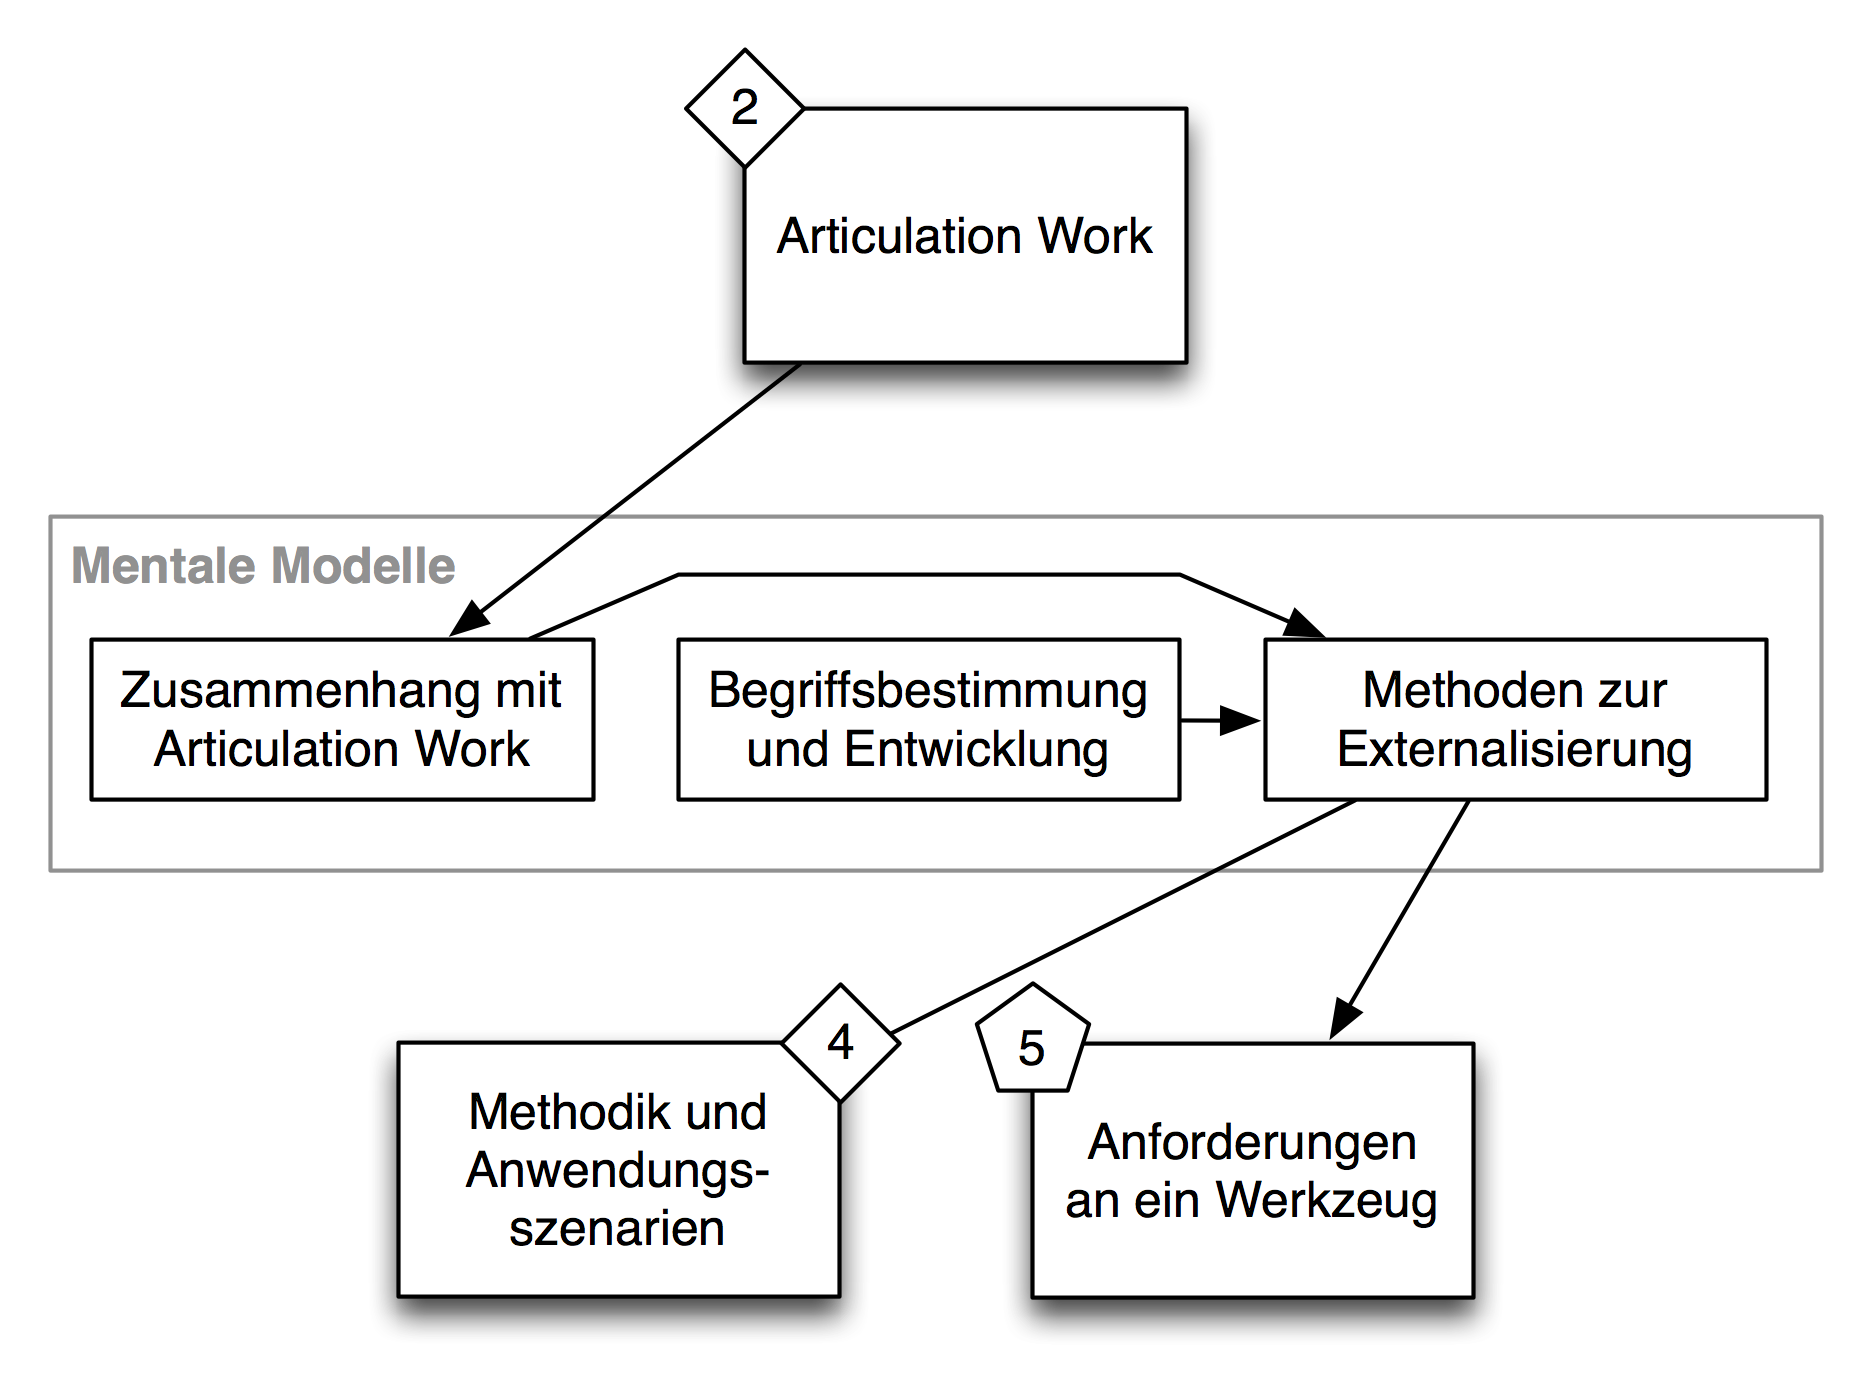
\includegraphics[scale=0.75]{img/Kontextgrafiken/k3.png}
	\caption{Kapitel „Mentale Modelle“ im Gesamtzusammenhang}
	\label{fig:img_Kontextgrafiken_k3}
\end{figure}

\section{Articulation Work und mentale Modelle} % (fold)
\label{sec:articulation_work_und_mentale_modelle}

Wie bereits im vorgehenden Kapitel beschrieben, werden in vorhandenen Arbeiten zu Articulation Work deren Auftreten, Kontext und Wirkung beschrieben, nicht aber jene Aspekte ihrer Durchführung, die die individuellen Aktivitäten betreffen. Der eigentliche Gegenstand der Abstimmung, die im Rahmen der Articulation Work erfolgen soll, wird ebenfalls nicht konkret festgelegt. Strauss spricht von \emph{„putting together tasks, task sequences, task clusters - even aligning larger units such as lines of work and subprojects - in the service of work flow“} \citep[][S. 2]{Strauss88}, und konkretisiert: \emph{„the specific questions about tasks of course include: what, where, when, how, for how long, how complex, how well defined are their boundaries, how attainable are they under current working conditions, how precisely are they defined in their operational details, and what is the expected level of performance. (Which of those are the most salient dimensions depends on the organizational work context under study, and we cannot emphasize too much that it is the researcher who must discover these saliences.)“} \citep[][S. 6]{Strauss85}. Strauss lässt also offen, was es exakt ist, dass abgestimmt werden muss bzw. verlagert diese Frage in den konkreten Einzelfall. 

Strauss spricht diese Auslassung in einer späteren Arbeit explizit an \citep[][S. 131]{Strauss93} und führt -- wie im letzten Kapitel bereits erwähnt -- das Konstrukt der „thought processes“ ein. Im Kontext der Abstimmung von Tätigkeiten kommt den „thought processes“ der Individuen insofern Bedeutung zu, als dass sie den sichtbaren individuellen Handlungen zugrunde liegen bzw. diese beeinflussen. „Articulation Work“ wirkt sich also auf die „thought processes“ der beteiligten Individuen aus. „Thought processes“ umfassen \emph{„images, imaginations, projections of scenes, [\ldots] flashes of insight, rehearsals of action, construction and reconstruction of scenarios,  the spurting up of metaphors or comparisons, the reworking and reevaluating of past scenes and one's actions within them, and so on and on“} \citep[][S. 130]{Strauss93} - also im Wesentlichen alle kognitiven Vorgänge, die unmittelbar oder mittelbar im Zusammenhang mit den sichtbaren Arbeitsaspekten, insbesondere den Tätigkeiten zur Zielerreichung und der wahrgenommenen Arbeitsumgebung, stehen. Strauss interessiert sich allerdings ausschließlich für die dynamischen Aspekte der Interaktion zwischen Individuen, nicht aber für die Ausgangspunkte und Ergebnisse der zugrunde liegenden „thought processes“ \citep[][S. 149]{Strauss93}.

% section articulation_work_und_mentale_modelle (end)

\section{Begriffsbestimmung} % (fold)
\label{sec:begriffsbestimmung}

% section begriffsbestimmung (end)

Das Konzept der „mentalen Modelle“ wird grundsätzlich verwendet, um zu erklären \emph{„wie Menschen die Welt verstehen -- genauer: wie sie ihr Wissen benutzen, um sich bestimmte Phänomene der Welt subjektiv plausibel zu machen“} \citep[][S. VII]{Seel91}. Mentale Modelle sind dabei Erklärungsmodelle der Welt, die von Menschen auf Basis von Alltagserfahrungen, bisherigem Wissen und darauf basierenden Schlussfolgerungen gebildet werden. Ein mentales Modell wird dann vom jeweiligen Individuum als Basis verwendet, um die Welt zu verstehen und ggf. Vorhersagen über deren Verhalten zu bilden. \citep[][S. VII]{Seel91}

Im Wesentlichen wurde das Forschungsfeld der mentalen Modelle durch zwei Arbeiten maßgeblich beeinflusst. \citet{Johnson-Laird81} sowie \citet{Kleer81} führen den Begriff als eigenständigen Forschungsgegenstand ein und legen damit die Grundlage für einen Großteil der nachfolgenden Arbeiten in dem Gebiet. Im Kontext dieser Arbeit wird auf das von \citet{Seel91} vorgeschlagene Verständnis von „mentalen Modellen“ zurückgegriffen. \citet{Seel91} versucht, die unterschiedlichen Richtungen der Forschung im Bereich der mentalen Modelle zusammenzuführen und daraus die Bedeutung von Mentalen Modellen für Lernvorgänge (unter die -- im breiten Verständnis von Seel -- auch die hier relevanten Abstimmungsvorgänge fallen) und Möglichkeiten zu deren Unterstützung abzuleiten. Die folgenden Ausführungen basieren deshalb auf den Ausführungen von \citeauthor{Seel91} und seiner Mitarbeiter (\citet{Ifenthaler06}, \citet{Pirnay-Dummer06} und \citet{Hanke06}).

Mentale Modelle sind nach \citet[][S. 7]{Ifenthaler06} \emph{„kognitive Konstruktionen, die abhängig von der jeweiligen Situation und vom semantischen Wissen einer Persone ad hoc konstruiert werden“}. Ein mentales Modell ist also kein permanentes kognitives Konstrukt, sondern wird auf Basis vorhandenen Wissens in bestimmten Situationen ad-hoc gebildet (siehe dazu auch Abschnitt \ref{sec:bildung_mentaler_modelle}). In engem Zusammenhang mit dem Begriff der mentalen Modelle ist jener der „Schemata“ zu nennen. „Schemata“ unterscheiden sich ihrer Definition nach nur in Detail von „mentalen Modellen“\footnote{Tatsächlich wird nach \citet{Ifenthaler06} der Begriff der „mentalen Modelle“ von manchen Autoren zugunsten von „Schemata“ als überflüssig bezeichnet, da zweitere die auftretenden kognitiven Phänomene ausreichend beschreiben würden.} Ein „Schema“ repräsentiert nach \citet[][S. 57]{Seel03a} \emph{„das aufgrund vielfältiger Einzelerfahrungen mit Objekten, Personen, Situationen und Handlungen erworbene verallgemeinerbare und abstrakte Wissen einer Person.“} Schemata werden benutzt um \emph{„Wissensstrukturen zu beschreiben, welche typische Zusammenhänge eines Realitätsbereiches repräsentieren.“} \citep[][S. 8]{Ifenthaler06}. Auf Basis dieser „Schemata“ treffen Individuen treffen Handlungsentscheidungen in bestimmten Situationen. „Schemata“ sind dabei als „Vorlagen“ zu sehen, die adäquate Handlungen für einen bestimmten Situationstypus vorgeben (im Sinne der erwähnten „Verallgemeinerbarkeit“) und Individuen damit zur raschen, unmittelbaren Handlung befähigt, ohne ausführliche Planungstätigkeiten durchführen zu müssen. In Abgrenzung dazu werden „mentale Modelle“ ad-hoc in Situationen gebildet, wo keine Schemata vorhanden sind oder vorhandene nicht angewandt werden können. 

\citet{Ifenthaler06} beschreibt den Zusammenhang zwischen Schemata und mentalen Modellen wie in Abbildung \ref{fig:img_MentaleModelle_iffenthaler_assimilation_akkommodation} dargestellt. Er bezieht sich dabei auf das „Äquilibrations“-Prinzip nach \citet{Piaget76}. Demnach entwickelt sich das Wissen eines Indiviuums durch die komplementären Prozesse „Assimilation“ und „Akkommodation.“

\begin{figure}[htbp]
	\centering		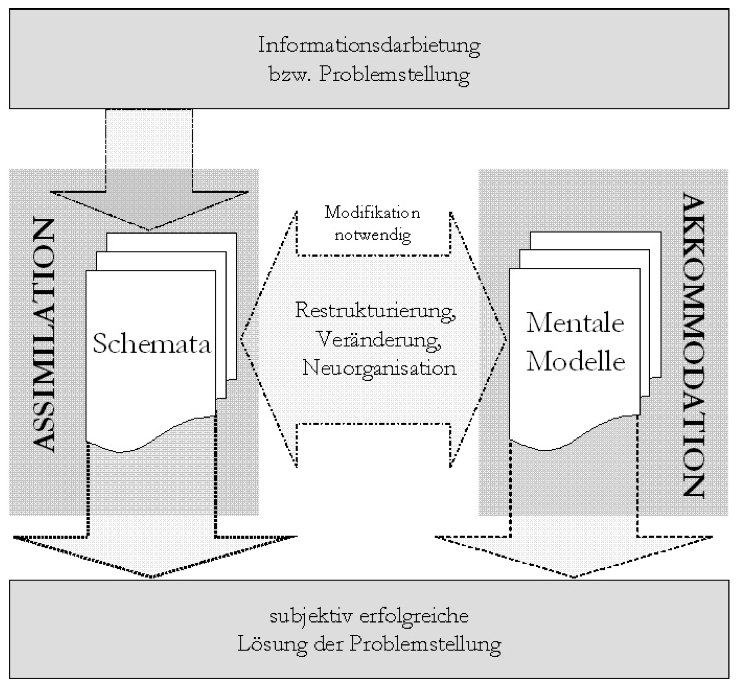
\includegraphics[height=3in]{img/MentaleModelle/iffenthaler_assimilation_akkommodation.png}
	\caption[Schemata und mentale Modelle]{Schemata und mentale Modelle (entnommen aus \citet[][S. 10]{Ifenthaler06})}
	\label{fig:img_MentaleModelle_iffenthaler_assimilation_akkommodation}
\end{figure}

Solange \wichtig eine wahrgenommene Situation auf existierende Schemata abgebildet werden kann und daraus unmittelbar Handlungen abgeleitet werden können, spricht man von „Assimilation“ der wahrgenommene Information. „Assimilation“ festigt bestehende Schemata, gestaltet diese ggf. in Details exakter aus oder um, stellt die grundlegenden Annahmen, die dem Schema zugrunde liegen, aber nicht in Frage. Kann die wahrgenommene Information nicht auf existierende Schemata abgebildet werden, kommt es zur „Akkommodation“, also der (ad-hoc) Bildung eines mentalen Modells und darauf aufbauend zur \emph{„Restrukturierung, Veränderung und Neuorganisation“} \citep{Ifenthaler06} der betreffenden Schemata. Schemata und mentale Modelle können damit auch als jene Strukturen interpretiert werden, die beim „Single-“ bzw. „Double-Loop-Learning“ nach \citet{Argyris78} zum Einsatz kommen. Im Kontext von „Articulation Work“ sind mentale Modelle in jenen Situation von Interesse, die als so „problematisch“ wahrgenommen werden, dass keine Fortführung der operativen Arbeit mehr möglich ist (auf individueller Ebene also evtl. existierende „Schemata“ nicht mehr zum Einsatz gebracht werden können). In diesen Situationen muss „explizite Articulation Work“ durchgeführt werden, um auf Basis eines mentalen Modells dieses selbst zu verändern, auszugestalten und soweit mit der Umwelt abzustimmen, das eine Wiederaufnahme der operativen Arbeit (bzw. die Bildung von adäquaten Schemata) möglich wird. Um auf die Durchführung von „expliziter Articulation Work“ unter Bezugnahme auf die mentalen Modelle der Individuen näher eingehen zu können, werden im nächsten Abschnitt die Bildung und Veränderung mentaler Modelle näher betrachtet.

\section{Bildung und Veränderung mentaler Modelle} % (fold)
\label{sec:bildung_mentaler_modelle}

Nach \citet{Seel91} umfasst die Bildung mentaler Modelle zwei Komponenten: Eine \emph{deklarative Komponente}, in der bereichs- bzw. domänen-spezifisches Wissen in der Form von hier nicht näher spezifizierten, strukturierten Wissensbasen abgelegt wird und eine \emph{operative Komponente}, in der auf Grundlage dieser Wissensbasen Schlüsse gezogen und neues Wissen abgeleitet wird, die über das ursprüngliche domänenspezifische Wissen hinausgeht. 

Das in den Wissensbasen repräsentierte Wissen kann auf Alltagserfahrung basieren oder durch Vermittlung oder Instruktion begründet werden. Im ersteren Fall ist das Wissen dann als konkret und handlungsbezogen anzusehen, im zweiten Fall ist das Wissen eher auf abstrakter, formaler Ebene anzusiedeln. Analog dazu kann auch in der operativen Komponente die Schlussfolgerung entweder induktiv auf Basis eines „intuitionsbegründeten“ Regelsystems gezogen werden oder durch Deduktion mittels einem formal begründbaren Regelsystem gebildet werden \citep{Seel91}. 

Die Modifikation und Erweiterung der eigenen Wissensbasen und die (Weiter-) Entwicklung der kognitiven Fähigkeiten, die für die Ableitung von Schlussfolgerungen notwendig sind, bezeichnet \citet{Seel91} als „Lernen“. Lernen ist \emph{"mit der Verarbeitung individueller Erfahrungen mit sowie vermittelter Information über die Welt, ihre Struktur und Evidenz verbunden und kann als ein Prozess permanenter konzeptueller Veränderungen verstanden werden."} \citep[][S. 23]{Seel91}. Lernen setzt damit die Fähigkeit und Bereitschaft voraus, \emph{"vermittelte Weltauffassungen zu verstehen, zu akzeptieren und sodann den eigenen gedanklichen Konstruktionen zugrunde zu legen"} \citep[][S. 23]{Seel91}. Im Wesentlichen entspricht dies einer Verallgemeinerung jener Vorgänge, die im Rahmen von nicht rein koordinierender sondern abstimmender und vor allem planender „Articulation Work“ durchgeführt werden.

In Zusammenhang mit diesem Verständnis von „Lernen“ sind verschiedene Arten von mentalen Modellen zu unterscheiden. \citet{Seel91} differenziert zwischen „Novizenmodellen“ und „Expertenmodellen“ (diese Unterscheidung trifft implizit auch \citet{Norman83a} im Kontext der Verwendung mentaler Modelle in der \gls{HCI}). Ein „Novizenmodell“ ist ein Alltagsmodell, dass ad-hoc in einer Problemsituation gebildet wird und dem Individuum, das es gebildet hat, in der aktuellen Situation plausibel erscheint (auch wenn es objektiv falsch ist). Es reicht aus, um adäquate Reaktionen auf die gegebene Situation abzuleiten, ohne das notwendigerweise eine Begründung der Handlungen möglich wäre oder diese nicht mit dem tatsächlichen Grund der Problembewältigung übereinstimmen\footnote{\emph{„[\ldots] most people’s understanding of the devices they interact with is surprisingly meager, imprecisely specified, and full of inconsistencies, gaps and idiosyncratic quirks.“}\citep[][S. 8]{Norman83a}}. Je öfter die Anwendung eines „Novizenmodells“ zum Erfolg führt, umso stabiler wird es zur Grundlage des Handelns des Individuums in der jeweiligen Situation. 

„Expertenmodelle“ (oder „wissenschaftliche Modelle“) sind hingegen inhaltlich vollständiger und bilden die Ursache-Wirkungs-Zusammenhänge der beobachtbaren Realität ab (sind also „objektiv korrekt“). Sie sind im allgemeinen differenzierter und bedienen sich einer adäquateren mentalen Codierung -- d.h. Begriffssystem -- als „Novizensysteme“ (die sich i.A. vertrauter Begriffssysteme bedienen, auch wenn diese einer anderen Domäne entstammen oder objektiv inkorrekt sind). Auch die Kompetenz des Individuums im Umgang mit dem mentalen Modell ist in diesem Fall höher. Der Übergang von einem „Novizenmodell“ zu einem „Expertenmodell“ erfolgt dabei durch „Lernen“ im oben genannten Sinn. \citep{Ifenthaler06}

„Expertenmodelle“ müssen aber nicht immer den erwünschten Endzustand eines Lernprozesses darstellen. Durch die gesteigerte Komplexität des Modells wird dessen ad-hoc-Anwendung schwieriger, die Nützlichkeit des Modells ist deshalb eingeschränkt \citep[vgl. ][S. 20]{Ifenthaler06}. Hier zeigt sich eine Analogie mit dem Bereich „Articulation Work“, wo es -- wie im letzten Kapitel beschrieben -- ebenfalls nicht als erforderlich angesehen wird, dass jedes beteiligte Individuum eine detaillierte Gesamtsicht auf den Arbeitsablauf hat. Vielmehr ist es ausreichend, die jeweils relevanten Schnittstellen zu abzustimmen und einen groben Überblick über den Gesamtzusammenhang zu haben. 

\citet{Ifenthaler06} erweitert deshalb die binäre Klassifikation durch „Erklärungsmodelle“, die er konzeptionell zwischen „Novizen-“ und „Expertenmodellen“ ansiedelt. Ein „Erklärungsmodell“ \emph{„beinhaltet alle notwendigen Informationen, um ein Problem bezüglich des Sachverhaltes und der Anforderungssituation richtig zu lösen. Einem Erklärungsmodell wird dabei ein hoher Grad an Nützlichkeit beigemessen, was in Bezug auf die kognitive Leistung zu einer ergonomischen Problemlösung führt. Je nach Komplexität des Sachverhaltes und der damit verbundenen Anforderungssituation kann ein Erklärungsmodell einem Novizenmodell oder einem Expertenmodell sehr ähnlich sein“} \citep[][S. 21]{Ifenthaler06}. „Erklärungsmodelle“ sind also je nach Art der zugrunde liegenden Problemstellung unterschiedlich aufgebaut. Ziel eines „Erklärungsmodells“ ist es immer, bestmöglich zur Problemlösung beizutragen, diese also für das Individuum im Kontext der jeweiligen Problemstellung möglichst einfach zu gestalten. Ein „Erklärungsmodell“ gewinnt dabei durch „Lernen“ an Reifegrad, es nähert sich einem „Expertenmodell“ immer weiter an.

Im \wichtig Kontext von „Articulation Work“ ist der Begriff des „Erklärungsmodells“ ein hilfreiches Konstrukt. Je nach Reifegrad des betreffenden mentalen Modells wird eine bestimmte Arbeitssituation als mehr oder weniger komplex wahrgenommen. Je komplexer eine Arbeitssituation wahrgenommen wird, desto größer ist der Bedarf nach expliziter „Articulation Work“, also der expliziten Beschäftigung mit dem Arbeitsprozess, dessen Reflexion und der Abstimmung der eigenen Wahrnehmung mit anderen beteiligten Individuen. Diese Beschäftigung mit dem Arbeitsprozess, also jene Tätigkeiten, die im Rahmen der „Articulation Work“ durchgeführt werden, entsprechen -- wie oben bereits beschrieben -- dem hier beschriebenen „Lernen“, wobei in kooperativen Arbeitssituation die Quellen „vermittelter Information“ vorrangig die anderen beteiligten Individuen oder organisationale Artefakte sind, die den Arbeitsablauf beschreiben. 

Die Veränderung mentaler Modelle weist zwei grundlegende Schwierigkeiten auf. Bei bereits als nicht adäquat erkannten mentalen Modellen (wie sie bei „Articulation Work“, die in „non-routine work“ bzw. „problematic work“ ausgeführt wird, auftreten), besteht grundsätzlich die Bereitschaft zur Veränderung (im Sinne einer „Akkommodation“ des mentalen Modells an die als verändert wahrgenommene Umweltbedingungen), die Herausforderung besteht aber darin, die notwendigen Informationen vermittelt zu bekommen, also an diese zu gelangen und adäquat dargeboten zu bekommen. Eine weitere Schwierigkeit ergibt sich in Situationen, in denen nicht alle involvierten Individuen die Situation als „problematisch“ wahrnehmen und deshalb keine grundlegende Bereitschaft zeigen, ihre der Arbeit zugrunde liegenden Annahmen (also ihre mentalen Modelle) zu verändern (\citet{Ifenthaler06} spricht von „hoher Veränderungsresistenz“). Dies tritt vor allem im Situationen auf, in denen „Articulation Work“ nicht aus einer allgemein wahrgenommen Problemsituation heraus durchgeführt wird, sondern entweder mit rein planendem Charakter angestoßen wird oder nur für einzelnen beteiligte Individuen so stark „problematisch“ ist, dass eine explizite Beschäftigung mehrerer oder aller am Arbeitsablauf beteiligten notwendig ist. 

Aus der Theorie der mentalen Modelle heraus begründet müssen also drei Rahmenbedingungen gegeben sein, um „explizite Articulation Work“ durchführen zu können:
\begin{enumerate}
	\item Die Beteiligten müssen bereit sein, ihre mentalen Modelle abzustimmen und das individuelle Verständnis der Schnittstellen abzugleichen.
	\item Die von den beteiligten Individuen benötigte Information über den Arbeitsablauf muss von den anderen Beteiligten zur Verfügung gestellt werden können oder in der Form organisationaler Artefakte vorliegen.
	\item Die benötigte Information muss in adäquater Form dargeboten werden, um  die individuellen mentalen Modelle mit diesen in Einklang zu bringen.
\end{enumerate}

Anforderung 1 ist eine Frage des sozialen Verhaltens der beteiligten Personen bzw. der Organisationskultur und kann ggf. durch organisationale Maßnahmen (z.B. durch die Förderung von „Communities of Practice“ \citep{Wenger99}) unterstützt werden. Anforderung 2 kann trivial zu erfüllen sein, wenn der Kontext des Arbeitsablaufs (d.h. das Umfeld, in dem die Arbeit durchgeführt wird, u.a. inkl. aller beteiligten Individuen) bekannt ist. In komplexen, neuartigen oder unbekannten Arbeitssituationen muss auch die Erfüllung dieser Anforderung unterstützt werden. Ansatzpunkte dafür liefert im Bereich von „Articulation Work“ etwa \citet{Grinter96} (siehe Abschnitt \ref{sub:supporting_articulation_work_using_software_configuration_management_systems}) oder \citet{Fuchs01} (siehe Abschnitt \ref{sub:teamspace}), umfassend mit dieser Thematik beschäftigt sich der Forschungsbereich der „Organisational Memories“ (zur technischen Unterstützung siehe etwa \citep{Abecker98} oder \citep{Diefenbruch02}\footnote{eine detaillierte Darstellung des Forschungsgebiets ist in \citep{Maier08} zu finden}).

Anforderung 3 wird in der Forschung zum Thema „Articulation Work“ von \citet{Sarini02} im Kontext des „alignment of meanings“ angesprochen, bei dem eine automationsgestützte Abbildung unterschiedlicher Domänenvokabulare die grundsätzliche Verständigung bzw. die Vermeidung von Missverständnissen vermeiden soll. Diese Maßnahme ermöglicht allerdings erst die Abstimmung mentaler Modelle, unterstützt diese aber noch nicht unmittelbar. Im Sinne der adäquaten Form der Darbietung argumentieren auch \citet{Divitini00}, \citep{Jorgensen04} und vor allem \citet{Herrmann02} mit der Forderung von flexiblen bzw. an die Bedürfnisse der Benutzer anpassbaren Modellierungsprachen bei der Verwendung von externalisierten Modellen als Unterstützung der Durchführung von „Articulation Work“ (siehe dazu die Abschnitte \ref{sub:supporting_different_dimensions_of_adaptability}, \ref{sub:interactive_process_models} und \ref{sub:modelling_cooperative_work}).

Hinsichtlich \wichtig Anforderung 3 argumentiert \citet{Seel91} im Bereich der mentalen Modelle für die Nützlichkeit externalisierter Repräsentationen zur Verbesserung von mentalen Modellen. Er vertritt die Auffassung, dass „die Externalisierung die Konstruktion eines mentalen Modells 'vervollkommnet'“, was er darauf zurückführt, dass „erst aus der Zielsetzung heraus, sich einem anderen mitzuteilen, die Präzision einer gedanklichen Konstruktion resultiert, die für die Erklärung einer Weltergebenheit erforderlich ist“ \citep[][S. 155]{Seel91}. Die Bildung von Externalisierungen mentaler Modelle verbessert also einerseits das individuelle mentale Modell, indem sie Lücken und Inkonsistenzen bewusst macht, und ermöglicht andererseits die Kommunikation mit anderen Individuen und ist damit die Grundlage der Vermittlung von Information und damit des „Lernens“ und „Articulation Work“ im hier beschriebenen Sinn. \citet{Seel91} lässt jedoch offen, in welcher Form die Repräsentation erfolgt, um die Vermittelbarkeit bestmöglich sicherzustellen\footnote{\emph{„Internalisierung von Erkenntnismitteln setzen Zeichensysteme (auditiver, visueller oder anderer Natur) für die Verschlüsselung der semantischen Gebilde voraus“}\citep[][S. 155]{Seel91}}. \citet{Ifenthaler06}, \citet{Hanke06} und \citet{Pirnay-Dummer06} weisen an dieser Stelle jedoch auf qualitative Unterschiede der Eignung unterschiedlicher externer Repräsentationsformen mentaler Modelle zur Externalisierung und Vermittlung derselben hin. Auf diese unterschiedlichen Formen und deren Eignung wird im nächsten Abschnitt eingegangen. 

Grundsätzlich konnte jedoch hier gezeigt werden, dass „Articulation Work“ die mentalen Modelle der beteiligten Individuen verändert bzw. auf diesen aufbaut. In weiterer Folge wurde deutlich, dass zur expliziten Durchführung von „Articulation Work“ auch aus der Theorie der mentalen Modelle heraus die Verwendung von externalisierten Modellen (wie bereits von \citet{Divitini00}, \citet{Herrmann02} und \citet{Jorgensen04} ohne den Hintergrund der mentalen Modelle vorgeschlagen) sinnvoll ist.

Diese Forderung nach einer Externalisierung mentaler Modelle, um deren Abstimmung zu unterstützten wird auch durch die Ausführungen von \citet{Senge90} und \citet{Kim93} gestützt, die mentale Modelle\footnote{in einem etwas breiteren Verständnis, welches im Wesentlichen auch Schemata umfasst: \emph{„[mental models are] deeply ingrained assumptions, generalizations, or even pictures and images that influence how we understand the world and how we take action.“}\citet{Senge90}} als ein wichtiges Konzept im Kontext des organisationalen Lernens identifizieren. Mentale Modelle bilden dort die Grundlage für Handlungen von Individuen in Organisationen und müssen geteilt werden, um der Organisation selbst eine Weiterentwicklung (einen „organisationalen Lernschritt“) zu ermöglichen.
% section bildung_mentaler_modelle (end)

\section{Externalisierung mentaler Modelle} % (fold)
\label{sec:externalisierung_mentaler_modelle}

Die Externalisierung von „mentalen Modellen“ ist immer ein zweistufiger Prozess (siehe Abbildung \ref{fig:img_MentaleModelle_iffenthaler_externalisierung}), in dem jeweils eine Transformation des Kodierungssystems stattfindet. Die wahrgenommene Realität (das „Weltwissen“) wird (ad-hoc) in ein mentales Modell abgebildet werden. Soll dieses externalisiert werden, ist dazu ein weiterer Übersetzungs- bzw. Abbildungsschritt notwendig. Gleichzeitig führt nach \citet{Stachowiak73} jede Modellbildung neben der „Abbildung“ auch zur „Verkürzung“, d.h. dass das Modell nicht die gesamte Information des Originals enthält, sondern nur jene Aspekte, die dem Ersteller relevant erscheinen\footnote{\emph{„Modelle erfassen im allgemeinen nicht alle Attribute des durch sie repräsentierten Originals, sondern nur solche, die den jeweiligen Modellerschaffern und/ oder Modellbenutzern relevant scheinen.“}\citep{Stachowiak73}}. In diesem Sinne können sie nur in einem bestimmten (zeitlichen, personellen und operationalen) Kontext für das Original stehen („pragmatisches Merkmal“ -- jedes Modells ist für einen bestimmten Zweck konstruiert\footnote{\emph{„Modelle sind ihren Originalen nicht per se eindeutig zugeordnet. Sie erfüllen ihre Ersetzungsfunktion: für bestimmte — erkennende und/ oder handelnde, modellbenutzende — Subjekte; innerhalb bestimmter Zeitintervalle und unter Einschränkung auf bestimmte gedankliche oder tatsächliche Operationen.“}\citep{Stachowiak73}}).

\begin{figure}[htbp]
	\centering
		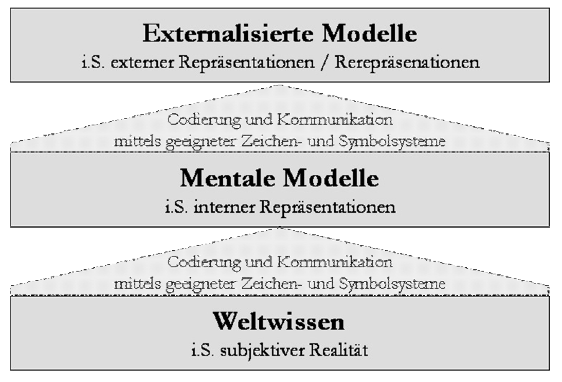
\includegraphics[width=8cm]{img/MentaleModelle/iffenthaler_externalisierung.png}
	\caption[Externalisierung mentaler Modelle]{Externalisierung mentaler Modelle (entnommen aus \citep{Ifenthaler06})}
	\label{fig:img_MentaleModelle_iffenthaler_externalisierung}
\end{figure}

Herausfordernd ist im Kontext von „Articulation Work“ das Abbildungsmerkmal, also die notwendige Übersetzungsleistung bei der Externalisierung eines mentalen Modells. Externalisierung umfasst nach \citet{Hanke06} immer die „Repräsentation“ als auch die „Kommunikation“ eines mentalen Modells. Die Relevanz dieser beiden Aspekte verschiebt sich je nach Kontext bzw. Zielsetzung der Externalisierung. Dient diese eher der individuellen Verständnisbildung, steht die „Repräsentation“ im Vordergrund (diesen Zweck erfüllt nach \citep{Seel91} auch bereits das mentale Modell selbst, die Externalisierung hat schärfenden Charakter). Die externalisierte Repräsentation soll nach \citet[][S. 187]{Seel91} in Bezug auf das repräsentierte mentale Modell
\begin{itemize}
	\item vollständig 
	\item konzise
	\item kohärent und konkret
	\item bedeutungshaltig und korrekt
\end{itemize}
sein. Das \wichtig Kodierungssystem muss hier also so gewählt werden, dass eine möglichst unmittelbare Abbildung der mentalen Modelle auf die externalisierte Repräsentation (und vice versa) möglich ist. 

In Situationen, in denen mentale Modelle zusätzlich auch anderen Individuen vermittelt werden sollen, steht „Kommunikation“ im Vordergrund. Die „Kommunizierbarkeit“ eines mentalen Modells hat Auswirkungen auf die wählbaren Kodierungssysteme zur Externalisierung. Das gewählte Kodierungssystem muss allen beteiligten Individuen verständlich sein, während dieses Kriterium bei der individuellen Verständnisbildung irrelevant ist \citep{Hanke06}. Im Rahmen von „Articulation Work“ steht im Allgemeinen die „Kommunikation“ bei der Externalisierung im Vordergrund, wobei diese ohne eine adäquate „Repräsentation“ nicht möglich ist. \label{anforderungen_seel} Ziel muss es also sein, Kodierungssysteme zur Verfügung zu stellen, die 
\begin{itemize}
	\item allen beteiligten Individuen verständlich sind, und
	\item eine möglichst unmittelbare Abbildbarkeit der mentalen Modelle auf die externalisierte Repräsentation ermöglicht.
\end{itemize}

Kodierungssysteme können \emph{„auditiver, visueller oder anderer Natur“} \citep[][S. 155]{Seel91} sein. Das gebräuchlichste Kodierungssystem ist die natürliche Sprache. Diese ist im Sinne der ersten Anforderung oft eine gute Wahl, bietet aber aufgrund ihrer Generizität nur wenig Möglichkeiten, sowohl den Repräsentations- als auch den Kommunikationsprozess bei der Externalisierung explizit zu unterstützen. \citet{Ifenthaler06} stellt mehrere Methoden vor, die sich spezifisch zum Zwecke der Externalisierung mentaler Modelle eignen und zu qualitativ höherwertigen Externalisierungsergebnisse führen sollen. Dies sind im Einzelnen:
\begin{itemize}
	\item Methode des lauten Denkens
	\item Strukturlegetechniken
	\item Concept Mapping
\end{itemize}

Auch \citep{Huss03} erwähnt diese Ansätze im Zusammenhang mit der Externalisierung „mentaler Repräsentationen“. In der Folge werden die genannten Ansätze detaillierter betrachtet. Dabei kommt folgender Raster zum Einsatz:
\begin{description}
	\item[Konzept] beschreibt die grundlegenden Konzepte des Ansatzes und die darauf aufbauende Zielvorstellung
	\item[Vorgehen] beschreibt, wie die Zielerreichung methodisch sichergestellt werden soll. 
	\item[Unterstützung] beschreibt, welche (technischen) Unterstützungsmaßnahmen vorgeschlagen werden.
	\item[Bewertung] fasst die Eigenschaften der Methode zusammen und beurteilt sie hinsichtlich ihrer Eignung für „Articulation Work“
\end{description}

\subsection{Methode des lauten Denkens} % (fold)
\label{sub:methode_des_lauten_denkens}

Die „Methode des lauten Denkens“ \citep{Van-Someren94} beschreibt ein Vorgehen, bei dem Individuen während ihrer operativen Tätigkeit ihre Gedanken und die Motive für ihr Handeln verbalisieren. 

\subsubsection{Konzept}

Die Grundidee des „Methode des lauten Denken“ basiert darauf, alle Gedanken, die im eine Tätigkeit begleiten, laut auszusprechen ohne sich auf diese Verbalisierung explizit zu konzentrieren (und etwa über Formulierungen nachzudenken oder Interpretationen durchzuführen). Es werden keine Fragen gestellt, das externalisierende Individuum wird ggf. lediglich daran erinnert, seine Gedanken auszusprechen. Nach \citet{Van-Someren94} hat diese Form der Externalisierung keinen negativen Einfluss auf die Durchführung der eigentlichen Tätigkeit.

Die „Methode des lauten Denkens“ wird immer mit dem Ziel durchgeführt, die kognitiven Prozesse in einer bestimmen Situation offenzulegen. Dazu muss eine Problemstellung ausgewählt werden, die diese Situation auslöst und möglichst keine oder geringe Nebeneffekte aufweist. Zu diesen Nebeneffekten gehört etwa die kognitive Überforderung des Individuums, wenn die Aufgabe als zu schwierig wahrgenommen wird. Gleichzeitig führt eine zu einfache Aufgabe zu eine routinisierten Abarbeitung, deren kognitiven Prozesse zumeist implizit und schwer zu externalisieren sind (vgl. „Operations“ in der „Activity Theory“ \citep{Leontev78}). Der wahrgenommene Schwierigkeitsgrad der Aufgabe steht in direktem Bezug mit der Expertise des Individuums (als unabhängige Variable), die damit bei der Auswahl der Problemstellung berücksichtigt werden muss.

Die „Methode des lauten Denkens“ wird oft mit Retrospektion kombiniert. Retrospektion ist die angeleitete Reflexion über eine Tätigkeit im Nachhinein (also nach Abschluss der Tätigkeit). Im Falle der Kombination mit der „Methode des lauten Denkens“ wird diese Reflexion mit Protokollen der verbalisierten Gedanken durchgeführt, was Unklarheiten in diesen Protokollen beseitigt und eine tiefergehende Reflexion ermöglichen kann. 

Die Ergebnisse der „Methode des lauten Denkens“ werden auf Basis von Audio- oder Video-Aufnahmen möglichst exakt transkribiert. Die Auswertung der Protokolle erfolgt im Normalfall nicht durch das Individuum selbst sondern wird interpretativ durch Dritte durchgeführt. Von \citet{Van-Someren94} wird dazu unter anderem vorgeschlagen, eine Aufgaben-Analyse durchzuführen, deren Ergebnis im Allgemeinen ein (diagrammatisches) Modell der Aufgaben und Tätigkeiten des Individuum zur Zielerreichung ist.

\subsubsection{Vorgehen}

\citet{Van-Someren94} beschreiben einen prototypischen Ablauf der „Methode des lauten Denkens“, der hier angegeben wird. Die Durchführung der Methode sollte in einer möglichst ungestörten, ruhigen Umgebung erfolgen. Das Individuum wird instruiert, bei der Problemlösung laut mitzusprechen und alles zu sagen, was ihm durch den Kopf geht (für konkrete Formulierungsvorschläge der Fragestellungen siehe \citep[][S. 43]{Van-Someren94}). Bevor die eigentliche Problemstellung bekannt gegeben wird, kann bei in der Methode ungeübten Individuen eine „Aufwärmphase“ durchgeführt werden, in der etwa anhand der Lösung einer einfachen Schlussrechnung das Verbalisierung der Überlegungen zu deren Lösung geübt werden kann.

Während der Durchführung der Methode beschränkt sich der Untersuchungsleiter darauf, das Individuum an das Aussprechen seiner Gedanken zu erinnern, sobald dieses zu sprechen aufhört. Der gesamte Verlauf der Aufgabenbearbeitung wird mittels Audio- oder Video-Ausrüstung aufgezeichnet.

Nach Abschluss der Methode wird die gesamt Aufzeichnung transkribiert. Bei der Transkription muss auf höchste Exaktheit geachtet werden, auch Sprechpausen oder nichtverbale Geräusche des Individuums sind relevant. Liegt eine Videoaufzeichnung vor, so wird das Transkript um die beobachteten Tätigkeiten des Individuums ergänzt. Das fertige Transkript kann dem Individuum im Sinne der Retrospektion zur Kommentierung vorgelegt werden, bei der Ergänzungen oder Erklärungen angebracht werden können (aber als solche gekennzeichnet werden müssen).

Zur Auswertung der Ergebnisse der „Methode des lauten Denkens“ werden unterschiedliche Methoden herangezogen, im im Detail in \citep{Van-Someren94} beschrieben sind. Da hier lediglich die Externalisierung selbst von Interesse ist, wird auf diese Methode an dieser Stelle nicht näher eingegangen.

\subsubsection{Unterstützung}

Eine technische Unterstützung der „Methode des lauten Denkens“ ist von den Entwicklern der Methode \citep{Van-Someren94} grundsätzlich nicht vorgesehen. Lediglich zur Dokumentation der artikulierten Information wird eine Aufzeichnung mittels Video- oder Audio-Ausrüstung empfohlen. Diese Dokumentation ist notwendig, um eine möglichst vollständige Auswertung der Information zu gewährleisten und eine Abbildung auf eine strukturierte Externalisierung des zugrunde liegenden mentalen Modells zu ermöglichen. 

\citet{Senge90} schlägt zur verbalen Externalisierung von mentalen Modellen einen Ansatz vor, der der „Methode des lauten Denkens“ nahe kommt, die Gedanken des Individuums aber verschriftlicht. Bei Einsatz der „left-hand column“\footnote{Eine detaillierte Beschreibung der Methode ist in \citep{Senge94} erschienen} wird ein Blatt Papier in zwei Spalten geteilt, wobei in der rechten Spalte eine Transkription der Handlungen bzw. der Konversation eines Individuums eingetragen wird. In der linken Spalte werden die Gedanken und handlungsmotivierenden Überlegungen eingetragen und den sichtbaren Handlungen in der rechten Spalte zugeordnet. Ein Nachteil dieser Methode ist, dass er -- auch wenn er technisch unterstützt werden würde -- nur im Nachhinein durchgeführt werden kann, um den eigentlichen Arbeitsablauf nicht zu unterbrechen.

\subsubsection{Bewertung}

Die „Methode des lauten Denkens“ \citep{Van-Someren94} ist die einzige der vorgeschlagenen Methoden zur Externalisierung mentaler Modelle, welche nicht auf eine graphische Repräsentationsform zurückgreift. Die externalisierende Person muss während der Aufgabenbearbeitung unmittelbar ihre kognitiven Prozesse und Denkmuster verbalisieren. Dies ist für viele Menschen ungewohnt und führt oft zu unvollständigen Repräsentationen. Detailliertes Nachfragen ist hier deshalb notwendig. Die gewonnen Daten (etwa aus Audio- oder Videomitschnitten des Versuchsszenarios) werden strukturiert ausgewertet, kategorisiert und interpretiert. Hier liegt auch die Schwierigkeit des Verfahrens -- in der Interpretation ist eine eindeutige Zuordnung zu bestimmten kognitiven Prozessen oft nicht möglich, die Repräsentation des mentalen Modells bleibt unvollständig oder ist inkonsistent. \citep[][S. 28]{Ifenthaler06}

In einer informellen Variante ist die „Methode des lauten Denkens“ jedoch vor allem für den Einsatz in nicht komplexen Fällen von „Articulation Work“ geeignet (also etwa bei kleineren Änderung im Arbeitskontext, die die Anpassung einzelner Tätigkeiten aber nicht die Adaption des gesamten Arbeitsablaufs benötigen). Dabei kann auf eine Aufzeichnung ggf. verzichtet werden, da die Durchführung der unmittelbaren Kommunikation dient und deren Ergebnisse nicht weiter interpretiert oder anderweitig verwendet werden müssen.

% subsection methode_des_lauten_denkens (end)

\subsection{Strukturlegetechniken} % (fold)
\label{sub:strukturlegetechniken}

Strukturlegetechniken sind Methoden, in denen gelegte Strukturen zur Repräsentation von „Wissen“ eingesetzt werden. Die gelegten Strukturen (die im Wesentlichen aus Knoten und Kanten unterschiedlicher Bedeutung bestehen) bilden dabei die Zusammenhänge einzelner Konstrukte ab, wie sie die legende Person wahrnimmt. Der Prozess des Legens ist eine \emph{„Rekonstruktion subjektiver Theorien“} \citep{Dann92} und stellt eine \emph{„[\ldots] verstehende Beschreibung von Handlungen nicht aus der Perspektive eines außenstehenden Beobachters, sondern aus Sicht der handelnden Person, des Akteurs selber“} \citep[][S. 2]{Dann92} dar.

\subsubsection{Konzept}

Das Konzept der Strukturlegetechniken entstammt im Wesentlichen einem Forschungsprogramm zur Entwicklung von Ansätzen zur „rekonstruktiven Erhebung subjektiver Theorien“ \citep{Dann92}. „Subjektive Theorien“ sind dabei im Wesentlichen den mentalen Modellen und Schemata gleichzusetzen\footnote{\emph{„Subjektive Theorien [\ldots] sind nicht nur unmittelbar handlungserklärend, -rechtfertigend oder –leitend; d.h. sie beziehen sich über die unmittelbare Erklärung/Rechtfertigung etc. eigener Handlungen hinaus auf z.B. ganze Handlungskategorien [\ldots]“} \citep[][S. 34]{Scheele88}} \citep[][zitiert nach \citep{Huss03}]{Kluwe90}. Strukturlegetechniken sind nicht als reine Erhebungsmethoden zu sehen, sondern beeinflussen durch den Lege-Vorgang selbst die zu externalisierenden mentalen Modelle und bilden damit die Grundlage für eine mögliche Veränderung des Agierens im Arbeitskontext \citep[][S. 6]{Dann92}.
Die Grundidee von Strukturlegetechniken ist die freie Anordnung und Assoziation von Begriffen. Je nach Variante kann dies individuell oder in Gruppen, mit oder ohne Moderator bzw. Untersuchungsleiter geschehen. Der Prozess ist dann abgeschlossen, wenn die Beteiligten die Repräsentation als eine adäquate Abbildung ihrer Denkmodelle sehen. Vor allem in kooperativen Sitzungen ist dies mit Aushandlungs- und Abstimmungsprozessen während der Repräsentation verbunden, was Strukturlegetechniken in der Durchführung potentiell aufwändig macht.

Strukturlegetechniken sind hinsichtlich der Art und dem Umfang der vorgegebenen Konstrukte nicht einheitlich aufgebaut. Es existieren Ansätze, in denen sämtliche Strukturelemente (also Konzepte und Arten von Beziehungen) vorgeben sind und die vom Externalisierenden „lediglich“ die Anordnung dieser Strukturelemente verlangen. Dem gegenüber stehen Strukturlege-Varianten, die weder die Konzeptklassen (und dementsprechend auch keine konkreten Konzepte) noch die Beziehungsarten vorgeben und deren Festlegung dem Externalisierenden überlassen (für einen Überblick über Varianten siehe \citep[][S. 29]{Ifenthaler06}). Im Fall der gängigen \gls{HSLT} \citep{Scheele88} wird ein zweistufiges Vorgehen gewählt, bei dem im ersten Schritt die Konzepte durch ein vorgegebenes Frageschema erhoben werden und im zweiten Schritt die Anordnung und Assoziation durchgeführt wird. Die Strukturen, die durch den Externalisierenden gebildet werden sind im Sinne von Stachowiaks „Allgemeiner Modelltheorie“ \citep{Stachowiak73} als „diagrammatische Modelle“ einzustufen (also ein im Normalfall graphisches, jedoch nicht ikonisches Darstellungsmodell).

\subsubsection{Vorgehen}

Je nach Variante von Strukturlegetechniken werden mehr oder weniger starke Vorgaben hinsichtlich des Ablaufs der Externalisierung gemacht. In der Literatur (z.B. \citep{Ifenthaler06}) wird die Dialog-Konsens-Methodik, die im Rahmen der Heidelberger Strukturlegetechnik \citep{Scheele88} zur Anwendung kommt, als einer der elaboriertesten Ansätze bezeichnet. Exemplarisch wird diese deshalb an dieser Stelle betrachtet.

Die Dialog-Konsens-Methodik sichert die Adäquatheit der während des Legeprozesses entstehenden mentalen Modelle durch laufende „kommunikative Validierung“ des Verständnisses ab. Um die kognitive Last zu reduzieren, wird dem eigentlichen Strukturlegeprozess eine Erhebungs-Phase vorgelagert, in der die relevanten Strukturelemente (Konzepte und Assoziationen) identifiziert werden. 

In der Erhebungsphase werden mittels einem semistrukturierten Interview (exemplarischer Aufbau siehe \citep{Scheele88}) werden Konzepte identifiziert, die für den jeweiligen Problembereich von Interesse sind. Die Identifikation erfolgt durch den Untersuchungsleiter auf Basis des Interview-Protokolls und nicht durch das externalisierende Individuum selbst. Das Individuum bestätigt, verändert oder erweitert in der Folge im Dialog mit dem Untersuchungsleiter die identifizierten Konzepte. Die Strukturierung der Konzepte erfolgt mittel vorgegebenen Relationen (die -- so wie die Konzepte -- als Kärtchen vorliegen). Die \gls{HSLT} definiert insgesamt 20 Relationsarten und sieht keine Erweiterung derselben vor. Die Strukturierung wird sowohl vom externalisierenden Individuum als auch von Untersuchungsleiter unabhängig voneinander vorgenommen und dann im Rahmen eines Dialog-Konsens-Prozesses gegenübergestellt und das Verständnis abgeglichen. Ziel ist hier, das der Untersuchungsleiter das mentale Modell des Indviduums versteht. \citet{Scheele88} schlagen vor, bei komplexen Sachverhalten die Konsensbildung über die Konzepte in einem separaten Dialog-Konsens-Prozess durchzuführen, bevor die Strukturierung vorgenommen wird.

Auch andere Strukturlegetechniken (siehe \citep{Dann92}) bleiben beim Konzept des Dialog-Konsenses und trennen zwischen der Phase der Konzepterhebung und der der Konzeptstrukturierung. Sie unterscheiden sich in der Zielsetzung der Externalisierung (und sind zum Teil nur für bestimmte Formen von mentalen Modelle geeignet) sowie im Grad der Vorstrukturierung (also inwieweit Konzepte und / oder Beziehungen bereits vorgegeben sind). Entsprechend der jeweiligen Offenheit bzw. Eingeschränktheit der Strukturlegetechnik ist die Phase der Konzept- (bzw. Beziehungs-)Sammlung mehr oder weniger stark ausgeprägt. Gemein ist allen Strukturlegetechniken, dass zwei dedizierte Phasen der Konzeptsammlung und der Konzeptstrukturierung durchgeführt werden, die in der Folge im Dialog-Konsens iterativ solange verfeinert werden, bis alle beteiligten Personen (also der Untersuchungsleiter und das externalisierende Individuum) mit dem Ergebnis zufrieden sind.

\subsubsection{Unterstützung}

Als technologische Unterstützung von Strukturlegetechniken wird in der Literatur mehrfach (u.a. bei \citep{Huss03} und \citep{Ifenthaler06}) die Software \gls{MaNET} \citep{Eckert98} erwähnt\footnote{http://www.marescom.net (Abruf am 21.08.2009)}. Von den Entwicklern dieses Produkts wird dieses aber wiederholt als Software zur computerunterstützten Generierung von „Concept Maps“ (siehe Abschnitt \ref{sub:concept_mapping}) bezeichnet. Tatsächlich verschwimmen ob der fehlenden physischen Repräsentation des Modells (es wird ausschließlich am Rechner konstruiert) und dem offenen semantischen Konzept (im Gegensatz zur \gls{HSLT}) die Grenzen zu „Concept Mapping“-Werkzeugen im Sinne der Entwickler dieses Ansatzes \citep{Novak06}. Ein ähnliches Bild zeigt sich bei \citet{Mandl00}, die bei der Unterstützung von Methoden zur „Strukturdarstellung“ auf „Concept-Mapping“-Werkzeuge verweisen.

Eine explizite Unterstützung des physischen Legeaspekts von Strukturlegetechniken wird in der Literatur nicht erwähnt. Aktuell existieren allerdings Bestrebungen, computerunterstützte „Concept Mapping“-Ansätze in den physischen Raum zu transferieren \citep{Do-Lenh09} \citep{Tanenbaum09}. Diese Ansätze werden in Abschnitt \ref{sub:aktuelle_verwandte_ansätze} im Rahmen der Beschreibung der verwandten Arbeiten genauer betrachtet.

\subsubsection{Bewertung}

Strukturlegetechniken bedienen sich einer physischen Abbildung der mentalen Modelle durch die externalisierende Person. Sie zählen damit hinsichtlich des Ergebnisses zu den graphischen Verfahren zur Externalisierung mentaler Modelle. Konzeptuell besteht keine Einschränkung auf individuelles Externalisieren, das Verfahren kann auch in Gruppen angewandt werden. Die beteiligten Personen bilden Begriffsnetzwerke, die die deren Handlungen zugrunde liegenden Annahmen und Modelle abbilden. Strukturlegetechniken werden in den gängigen Varianten durch Dialog-Konsens-Methoden unterstützt, in denen die Modelle in Interaktion zwischen dem Externalisierenden und dem Moderator bzw. Versuchsleiter entstehen. Grundsätzlich ist dies aber nicht notwendig und wird auch nicht in allen Strukturlege-Varianten angewandt.

Hinsichtlich der Auftrennung des Externalisierungsprozesses in zwei Phasen (Konzept-Sammlung und –Strukurierung) erscheint bei der Durchführung im Rahmen von „Articulation Work“ eine fakultative Durchführung der ersten Phase möglich und angemessen. Durch die inhaltliche Offenheit von „Articulation Work“ sind viele Konstrukte nur in ihrem Kontext sinnvoll verständlich und müssen deshalb unmittelbar in die Struktur eingebettet werden oder werden erst aus dieser ersichtlich. Eine strikte Teilung in Sammlung und Strukturierung ist daher in diesem Anwendungsbereich fragwürdig. Bei der Modellierung komplexer Zusammenhänge scheint außerdem eine möglichst hohe Flexibilität der Repräsentationsform von Vorteil zu sein, um den Modellierungsprozess nicht zur behindern und eine Fokussierung auf den Modellierungsgegenstand zu ermöglichen \citep[][S. 6]{Goguen93}. Dies wird im Kontext von „Articulation Work“ \citep[][S. 10]{Schmidt00} und insbesondere bei der Verwendung von diagrammatischen Modellen zu diesem Zweck \citep[][S. 23]{Jorgensen04} als wesentlich erachtet. 

Im Falle von „Articulation Work“ ist von einer wechselseitigen Abstimmung der mentalen Modelle der beteiligten Individuen auszugehen (obgleich es Szenarien geben kann, in der klassische Experten-Laien-Settings im Sinne eines unidirektionalen Wissenstransfers auftreten – diese werden hier jedoch als Spezialfall des allgemeinen, wechselseitigen Szenarios betrachtet). Dazu ist eine Auflösung der in der ursprünglichen Methode vorgesehenen strikten Trennung zwischen „Proband“ und „Untersuchendem“ hin zu einer gleichberechtigten Rolle aller Beteiligten notwendig. Zu untersuchen bleibt, ob die Rolle des Moderators und „Ermöglichers“ (im Sinne der Unterstützung bei der Werkzeugbenutzung), die ansonsten vom Untersuchungsleiter eingenommen wird, nach wie vor explizit wahrgenommen werden muss (durch eine Person, die ansonsten nicht in den Dialog-Konsens-Prozess eingebunden ist).

Kritisch betrachtet wird die lange Durchführungsdauer der Externalisierungs-Prozesse, die eine nicht unwesentliche Belastung der Teilnehmer darstellt. Auch die Komplexität mancher Ansätze (etwa der \gls{HSLT} mit ihren 20 unterschiedlichen Beziehungstypen) stellt eine nicht unwesentliche kognitive Belastung der Teilnehmer dar.  Neuere Ansätze empfehlen zur Reduktion des Aufwandes den Einsatz von rechnerbasierten Werkzeugen, ohne dabei jedoch spezifischer zu werden. \citep[][S. 29f]{Ifenthaler06}
% subsection strukturlegetechniken (end)

\subsection{Concept Mapping} % (fold)
\label{sub:concept_mapping}

Concept Mapping \citep{Novak06} ist eine Methode, in der semantische offene diagrammatische Modelle graphisch erstellt werden. Sie dienen der flexiblen Abbildung von Begriffen (Konzepten) und deren Zusammenhänge. Die erstellte Struktur entspricht einem Graphen mit Knoten, die die Konzepte repräsentieren und Kanten, die gerichtet oder ungerichtet die Beziehungen zwischen den Konzepten herstellen und durch Beschriftung zusätzlich spezifiziert werden können. Concept Mapping sollte ob der potentiellen Komplexität der entstehenden Modelle \citet{Novak06} zufolge durch rechnerbasierte Werkzeuge unterstützt werden. 

\subsubsection{Konzept}

Concept Maps sind graphische Strukturen, in denen durch Knoten und Kanten Begriffe und deren Zusammenhänge dargestellt werden. Die Begriffe („Konzepte“) werden dabei anhand des Themas der Concept Map ausgewählt, die zumeist in Form einer Fokus-Frage vorliegt. Ein Konzept ist nach \citep[][S. 1]{Novak06} \emph{„a perceived regularity in events or objects, or records of events or objects, designated by a label“}. Konzepte sind also allgemeine Aussagen über Phänomene oder Objekte, die durch einen Bezeichner beschrieben werden können. Diese Bezeichner sind im Allgemeinen kurz und sollten 1-2 Worte umfassen.

Die Konzepte werden untereinander mit Beziehungen verbunden, wobei die Kombination aus zwei oder mehreren Konzepten und einer Beziehung als „Proposition“ bezeichnet wird. „Propositioen“ sind nach \citet[][S. 1]{Novak06} \emph{„statements about some object or event in the universe, either naturally occurring or constructed“}. Beziehungen können grundsätzlich gerichtet oder ungerichtet sein und müssen durch eine Beschriftung („linking word“) mit (beliebiger) Bedeutung versehen werden. Nach \citet{Novak06} enthalten Concept Maps meist eine hierarchische Struktur, in der die allgemeinen Konzepte am oberen Rand angeordnet sind und nach unten hin immer spezifischer werden. Daneben gibt es „cross-links“, die Beziehungen außerhalb der hierarchischen Struktur darstellen und Konzepte zueinander in Beziehung setzen, die in unterschiedlichen Bereichen der Concept Map stehen. Die grundlegende Struktur eine Concept Map ist in Abbildung \ref{fig:img_MentaleModelle_novak_concept_maps} als Concept Map dargestellt.

\begin{figure}[htbp]
	\centering
		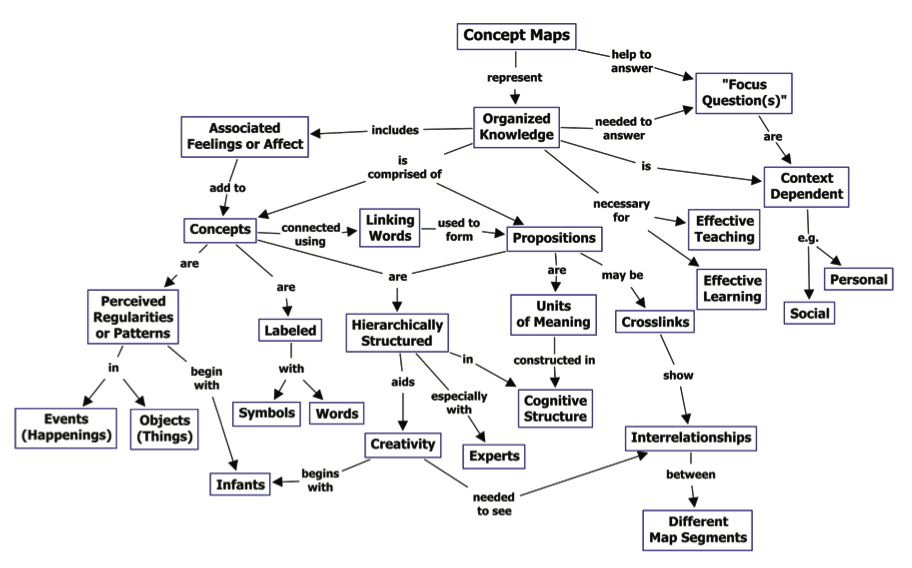
\includegraphics[width=12cm]{img/MentaleModelle/novak_concept_maps.png}
	\caption[Struktur einer Concept Map]{Struktur einer Concept Map (entnommen aus \citep[][S. 2]{Novak06})}
	\label{fig:img_MentaleModelle_novak_concept_maps}
\end{figure}

Concept Maps werden verwendet, um exploratives Lernen zu unterstützen. In diesem Fall bilden Individuen die ihnen bewussten Zusammenhänge der Realität in der Concept Map ab und erschließen bei der individuellen oder kooperativen Erstellung den Problembereich vollständiger, was zur Entwicklung eines umfassenderen Verständnisses beiträgt. Nach \citet{Novak06} können Concept Maps auch verwendet werden, um (implizites) Expertenwissen abzubilden (die Autoren beziehen sich hier auf die „Wissenspirale“ nach \citet{Nonaka95}. Im Wesentlichen ermöglichen Concept Maps damit das Externalisieren sowohl von Laien- als auch Expertenmodellen im Sinne von \citet{Seel91} und unterstützen auch die Weiterentwicklung von Laienmodellen hin zu ausgereifteren Erklärungs- oder Expertenmodellen.  Damit ist eine grundsätzliche Eignung für den Einsatz im Rahmen von auf der Externalisierung von Modellen basierender „Articulation Work“ gegeben.

\subsubsection{Vorgehen}

\citet{Novak06} schlagen vor, bei der Konstruktion einer Concept Map mit der Festlegung einer Fokus-Frage zu beginnen. Die Fokus-Frage muss klar formuliert sein und spezifisch auf das Problem oder den Sachverhalt eingehen, der in der Concept Map repräsentiert werden soll. Die Fokus-Frage dient nicht nur der Festlegung des Gegenstands der Concept Map sondern auch deren Abgrenzung nach außen (d.h. dass die Frage so spezifisch sein muss, dass Abweichungen vom intendierten Gegenstand der Concept Map erkannt werden können).

Im nächsten Schritt werden die relevanten Konzepte gesammelt. \citet{Novak06} sprechen von 15-25 Konzepten, die im ersten Durchlauf maximal verwendet werden sollten. Diese Konzepte können grob entsprechend ihrer Abstraktheit vorsortiert werden, um die Erstellung der Concept Map im nächsten Schritt zu erleichtern.

Die vorläufige Concept Map, die im nächsten Schritt erstellt wird, basiert auf den hierarchischen Zusammenhängen zwischen den gesammelten Konzepten. Zwischen diesen wird in der Folge nach „cross-links“ gesucht. Alle identifizierten Beziehungen müssen benannt werden. Im Zuge dieser ersten Herstellung von Beziehungen ergeben sich im Normalfall weitere Konzepte, die in die Concept Map aufgenommen werden müssen. Dies erfolgt im Zuge eines erneuten Durchlaufs durch den beschriebenen Prozess. Nach \citet{Novak06} benötigt eine Concept Map mindestens drei dieser Durchläufe, um ausreichende Qualität erreichen zu können.

\subsubsection{Unterstützung}

\citet{Novak06} erwähnen, dass Concept Mapping mittels Haftnotizen auf Papier oder Whiteboards durchgeführt werden kann, empfehlen aber, ein rechnerbasiertes Werkzeug -- die CMapTools \citep{Canas04} -- einzusetzen, dass den Erstellungsprozess unterstützt und den Umgang mit der entstehenden Komplexität erleichtert.

Dieses Werkzeug ermöglicht neben der Unterstützung des Mapping-Prozesses (d.h. der Nachverfolgung des Prozesses und der Möglichkeit, einzelne Schritte rückgängig zu machen) auch eine erweiterte Abbildung der Concept Map selbst. Diese umfasst unter anderem auch die Einbindung von externen Ressourcen (Dateien am Rechner), was von \citet{Novak06} als Wesentlich zur Einbettung der Concept Map in den Kontext des Problemumfelds angesehen wird.

\subsubsection{Bewertung}

Concept Mapping ist ein Ansatz zur computer-basierten Strukturierung und Visualisierung von Konzept-Netzwerken \citep{Novak06}. Durch die Rechnerunterstützung ergeben sich Vorteile hinsichtlich der Flexibilität der Darstellung und der Archivierung der Modelle. Konzeptuell werden wie bei Strukturlegetechniken Begriffsnetzwerke gebildet, wobei die methodische Hinterlegung bei Concept Mapping Ansätzen nicht so variantenreich und detailliert ausgeführt ist. 

Durch die digitale Repräsentation ist eine Concept Map leichter ohne Konsequenzen zu manipulieren, da Änderungen jederzeit rückgängig gemacht werden können. Dies ermöglicht Experimente mit dem Modell und erlaubt dem Externalisierenden eine umfassendere Ergründung und Reflexion der Modelle. Kritisch wird jedoch die im Gegensatz zu Strukturlegetechniken fehlende Unmittelbarkeit der Externalisierung betrachtet – jeder Externalisierung-Prozess muss am Rechner umgesetzt werden und setzt damit Kompetenz im Umgang mit diesem Medium voraus. \citet[][S. 30f]{Ifenthaler06}

Für die Durchführung von „Articulation Work“ erscheinen Concept Maps durch ihre semantische Offenheit vor allem zur expliziten Unterstützung von „alignment of meaning“ (vgl. \citep{Sarini02}, beschrieben in Abschnitt \ref{sec:arten_von_articulation_work}). Bei der rechner-gestützten Durchführung von Concept Mapping ist aber die Wirkung der auf einen Benutzer ausgerichteten Benutzungsschnittstelle (Monitor sowie Maus und Tastatur) auf die Interaktion zwischen den Beteiligten zu berücksichtigen.

% subsection concept_mapping (end)

% section externalisierung_mentaler_modelle (end)

\section{Zusammenfassung} % (fold)
\label{sec:mentale_modelle_fazit}

In diesem Kapitel wurde das Konzept der „Mentalen Modelle“ eingeführt und dessen Relevanz für die Durchführung expliziter „Articulation Work“ beschrieben. In weiterer Folge wurden die Externalisierung mentaler Modelle, deren Rückwirkung auf die kognitven Prozesse der Individuen sowie Methoden zu Unterstützung des Externalisierungsvorganges beschrieben. Der Zusammenhang des Themenbereichs der „Mentalen Modelle“, deren Externalisierung und deren Einbettung in den Gesamtzusammenhang von „Articulation Work“ ist in Abbildung \ref{fig:img_MentaleModelle_ArbeitInteraktionMentaleModelle} nochmals zusammenfassend dargestellt.

\begin{figure}[htbp]
	\centering
		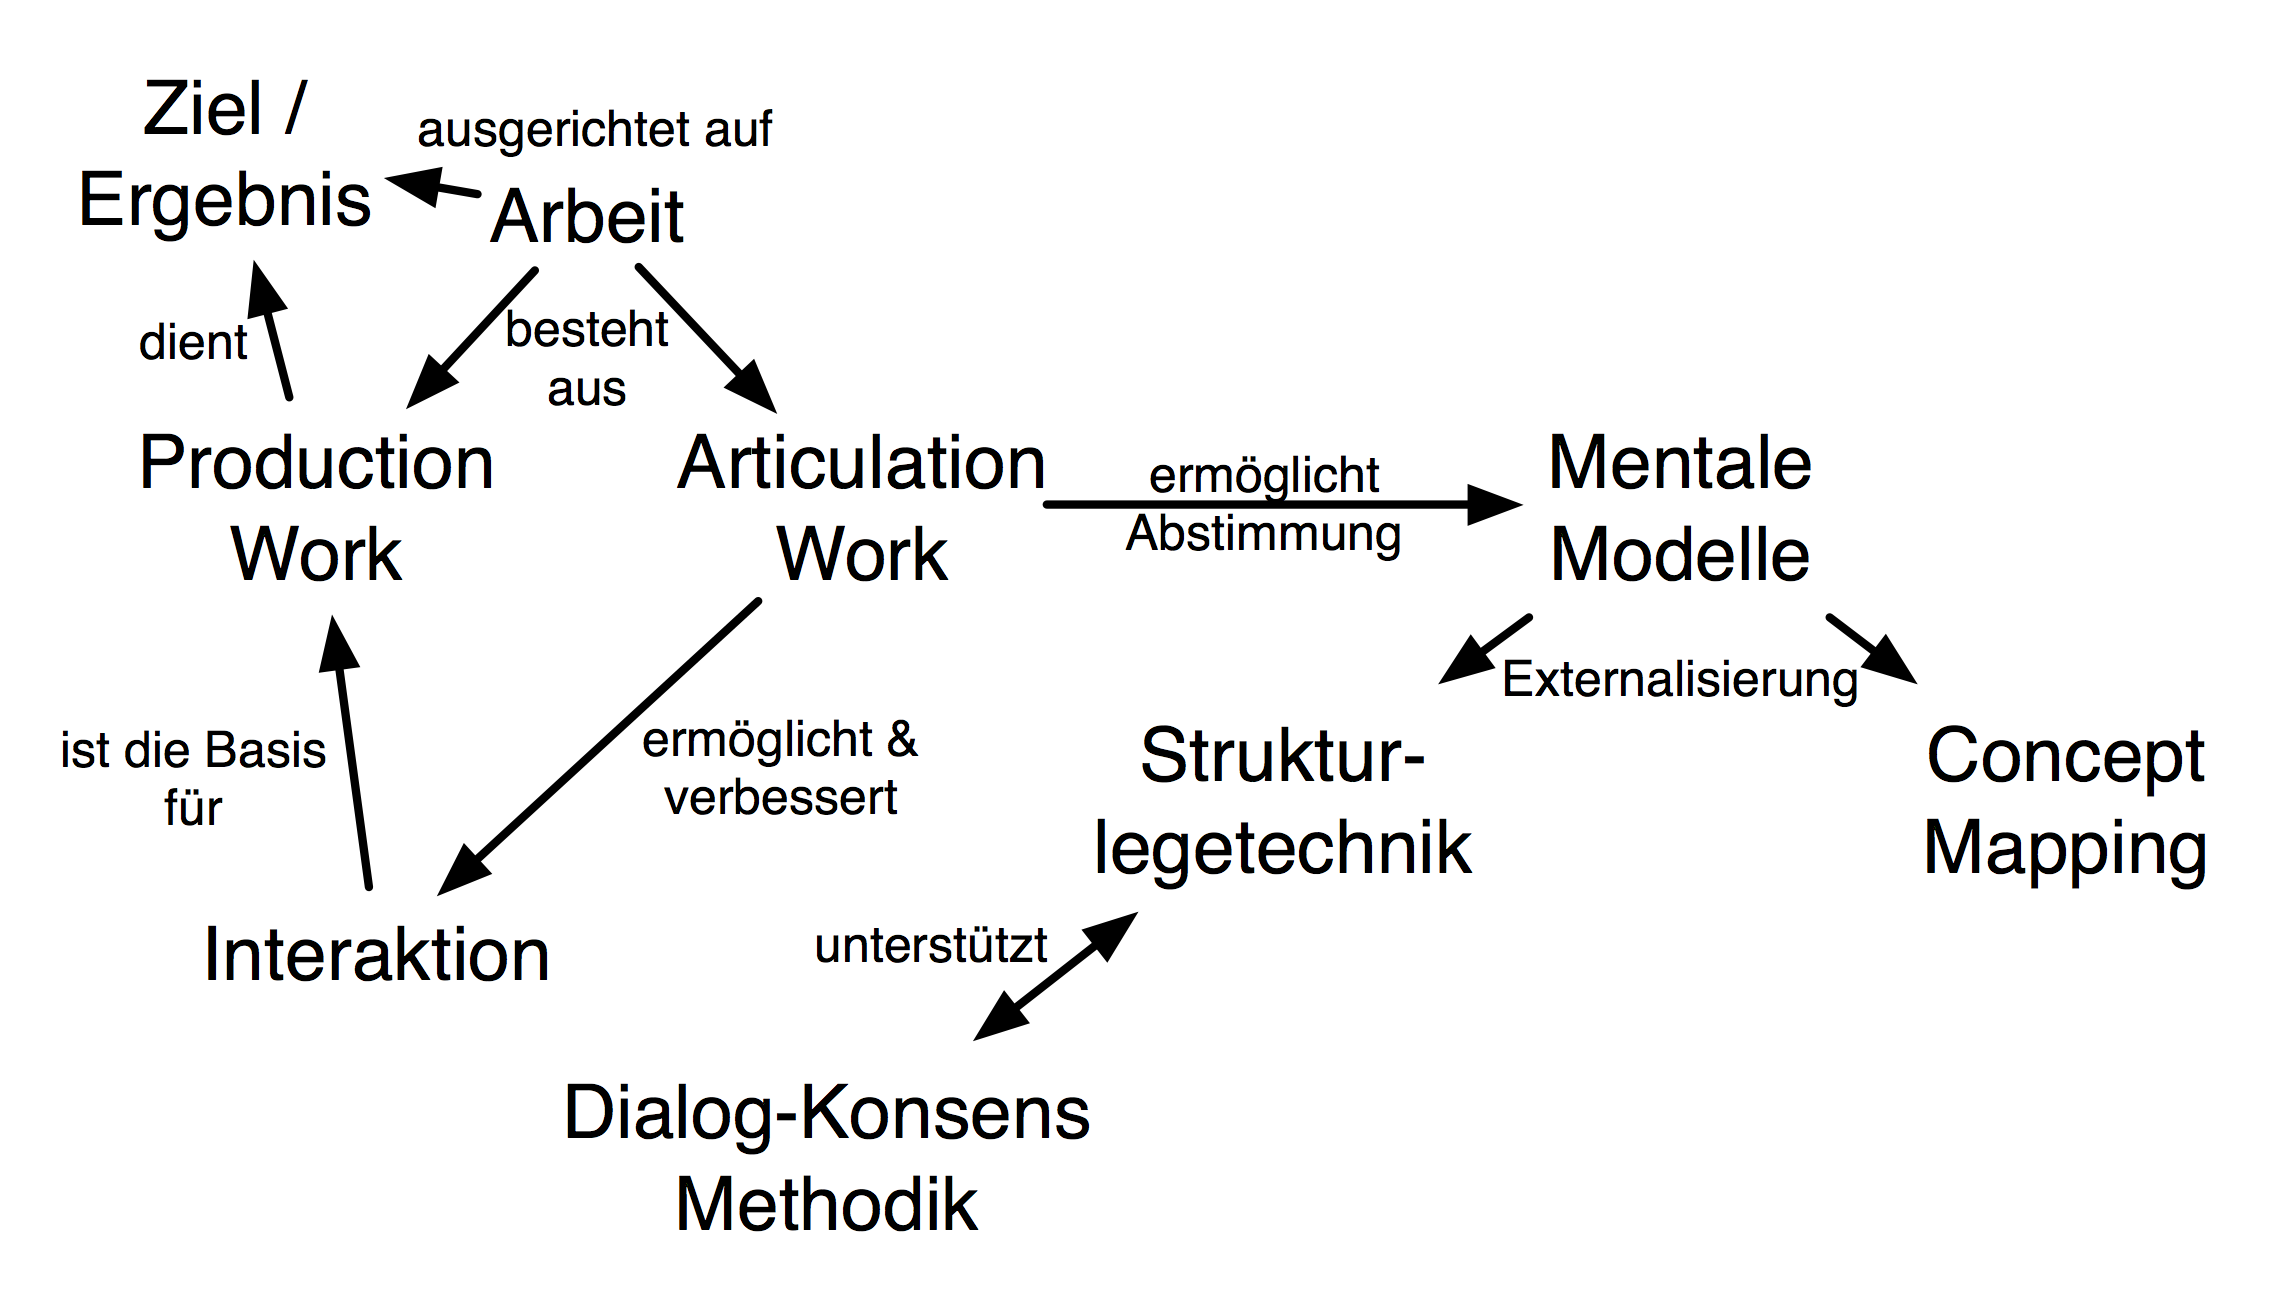
\includegraphics[width=10cm]{img/MentaleModelle/ArbeitInteraktionMentaleModelle.png}
	\caption{Mentale Modelle und Articulation Work im Gesamtzusammenhang}
	\label{fig:img_MentaleModelle_ArbeitInteraktionMentaleModelle}
\end{figure}


„Mentale Modelle“ sind ein Erklärungskonzept für jene mentalen Strukturen und Vorgänge, mit Hilfe derer Individuen ihre Wahrnehmungen der realen Welt erklären und Handlungsalternativen ableiten. Durch Lernprozesse können „Mentale Modelle“ verfeinert oder grundlegend verändert werden. Quellen für neue Information, die in mentalen Modellen abgebildet wird, können die Wahrnehmung der realen Welt, dokumentarische Ressourcen oder andere Individuen sein. Ein wesentlicher Unterstützungsfaktor für die Reflexion und Verfeinerung mentaler Modelle ist deren Externalisierung. Diese ist außerdem die Voraussetzung für die Kommunikation und Abstimmung verschiedener mentaler Modelle.

Während die Externalisierung auch rein verbal erfolgen kann, ist die Verwendung einer expliziten, graphischen Repräsentation vorteilhaft. Diese wirkt vor allem in Situationen, in denen mentale Modelle offengelegt und kommuniziert werden sollen, als Ankerpunkt und Dokumentation, anhand derer eine Abstimmung der individuellen Sichten erfolgen kann. Methoden, deren Eignung zur Externalisierung mentaler Modelle empirisch belegt ist, sind unter anderem Strukturlegetechniken und Concept Mapping. Für die im Rahmen dieser Arbeit verfolgte Unterstützung von „expliziter Articulation Work“ bieten beide Methoden Vor- und Nachteile. Deswegen wird im folgenden Kapitel eine Synthese dieser beiden Methoden angestrebt, die deren Vorteile vereint und gleichzeitig die nachteilig wirkenden Faktoren zu vermeiden sucht.

% section fazit (end)

% chapter mentale_modelle (end)

% \chapter{Mentale Modelle}
% \label{cha:mentale_modelle}
% 
% In diesem Kapitel wird das Konzept der mentalen Modelle eingeführt, das in dieser Arbeit als Erklärungsansatz für jene Aspekte von "Articulation Work" verwendet wird, die die nicht sichtbaren, kognitiven Beiträge eines beteiligten Individuums betreffen. Nach einer Einführung in die Begriffswelt der mentalen Modelle wird die Argumentation aus dem letzten Kapitel nochmals aufgegriffen und die mögliche Rolle mentaler Modelle für "Articulation Work" erörtert. In der Folge werden Methoden eingeführt mit denen mentale Modelle externalisiert und kommuniziert werden können. Basierend auf diesen Beschreibungen wird im letzten Teil des Kapitels untersucht, welche Herausforderungen sich bei der Anwendung dieser Methoden im Kontext von "Articulation Work" ergeben können.
% 
% \section{Begriffsbestimmung}e
% \label{sec:mentalemodelle_begriffsbestimmung}
% 
% Der Begriff der Mentalen Modelle wurde von \citet{Johnson-Laird81} geprägt. Ein mentales Modell ist nach 
% 
% \subsection{Mentale Modelle nach Johnson-Laird} % (fold)
% \label{sub:mentale_modelle_nach_johnson_laird}
% 
% % subsection mentale_modelle_nach_johnson_laird (end)
% 
% \subsection{Mentale Modelle nach Norman} % (fold)
% \label{sub:mentale_modelle_nach_norman}
% 
% \citet{Norman83a} formuliert ein Verständnis von mentalen Modellen aus Interaktionssicht. Sein Kontext ist die Untersuchung von Mensch-Maschine-Interaktion und den dort auftretenden Interaktionsabläufen. Mentale Modelle sind in diesem Verständnis individuelle Konstrukte, die von Menschen bei der Interaktion mit der Umwelt, mit anderen Menschen oder mit Technologie gebildet werden, um das Verhalten der Gegenseite erklären und vorhersagen zu können\footnote{\emph{„In interaction with the environment, with others, an with the artifacts of technology, people form internal, mental models of themselves and of the things with which they are interacting. These models provide predictive and explanatory power for understanding the interaction“} \citep{Norman83a}}. Um den Begriff abzugrenzen, führt \citeauthor{Norman83a} ein aus vier Elementen bestehendes Begriffssystem ein, das den Diskussionsbereich abgrenzt und definiert:
% \begin{description}
% 	\item[target system] Das Zielsystem ist jenes System, das von einer Person benutzt wird oder dessen Benutzung von dieser Person erlernt wird.
% 	\item[conceptual model of target system] Ein konzeptionelles Modell ist ein Modell, dass das Zielsystem vollständig, konsistent und exakt beschreibt. Konzeptionelle Modelle werden von Entwicklern, Designern, Wissenschaftern oder Lehrern (im Allgemeinen: Experten in der Domäne des Zielsystems) definiert.
% 	\item[mental model of target system] Mentale Modelle werden von Personen bei der Interaktion mit dem Zielsystem entwickelt, um dessen Verhalten zu erklären. Diese Modelle müssen nicht vollständig und exakt sein, müssen aber für die jeweilige Person funktional sein, d.h. für deren Zwecke ausreichendes Erklärungspotential besitzen. Mentale Modelle haben evolutionären Charakter und entwickeln sich während der Interaktion mit dem System weiter. Die Inhalte eines mentalen Modells werden durch das Vorwissen und die Erfahrung der jeweiligen Person beeinflusst.
% 	\item[scientist's conceptualization of mental model] Die Konzeptualisierung eines mentalen Modells ist der Versuch ein mentales Modell mit wissenschaftlichen Mitteln zu erheben und abzubilden. Sie soll die Inhalte des mentalen Modells möglichst vollständig und genau abbilden. Die Konzeptualisierung ist also ein Modell eines Modells.
% \end{description}
% 
% Im Weiteren nennt \citeauthor{Norman83a} sechs generelle Eigenschaften von mentalen Modellen, die er aus eine Vielzahl von Beobachtungen in unterschiedlichen Kontexten ableitet:
% \begin{enumerate}
% 	\item Mentale Modelle sind unvollständig
% 	\item Mentale Modelle können von ihren Trägern nur sehr einschränkt wiedergegeben werden.
% 	\item Mentale Modell sind instabil und werden vor allem in Bereich ungenau, die Teile des Zielsystems abbilden die lange nicht benötigt wurden.
% 	\item Mentale Modelle sind nicht klar voneinander abgrenzbar -- ähnliche Gegenstände oder Situationen werden oft hinsichtlich der angewandten Interaktionsmuster verwechselt.
% 	\item Mentale Modelle sind unwissenschaftlich -- auch mentale Modelle, die inhaltlich (technisch) überflüssiges Verhalten verursachen, werden beibehalten, wenn der Aufwand der physischen Ausführung gering ist.
% 	\item Mentale Modelle sind simpel -- auch wenn eine effizientere Interaktion möglich wäre, wenn mehr Aufwand in die Planung investiert würde bzw. ein komplexeres mentales Modell zum Einsatz käme, präferieren Benutzer einfache Modelle, deren Anwendung höheren „physischen Aufwand“ mit sich bringen.
% \end{enumerate}
% 
% % subsection mentale_modelle_nach_norman (end)
% 
% \subsection{Mentale Modelle nach Senge} % (fold)
% \label{sub:mentale_modelle_nach_senge}
% 
% % subsection mentale_modelle_nach_senge (end)
% 
% \section{Veränderung mentaler Modelle}
% \label{sub:veränderung_mentaler_modelle}
% Assimilation vs. Akkommodation
% 
% \section{Mentale Modelle und Articulation Work}
% \label{sec:mentale_modelle_und_articulation_work}
% 
% Argumentation mit Wissensspirale (Nonaka \& Takeuchi)

\chapter{Methodik und Anwendungszenarien} % (fold)
\label{cha:methodik}

In diesem Kapitel wird die Methodik vorgestellt, die zur Externalisierung von mentalen Modellen mit dem zu entwickelnden Werkzeug zur Anwendung kommt. Die Inhalte dieses Kapitels bauen auf den Ergebnissen der Kapitel \ref{cha:articulation_work}  und \ref{cha:mentale_modelle} auf. Die Anforderungen, die sich auf der hier vorgestellen Methodik ergeben, werden in Kapitel \ref{cha:anforderungen} identifiziert und in weiterer Folge in einem Werkzeug umgesetzt.

Basierend auf den Schlussfolgerungen, die \citet{Ifenthaler06} hinsichtlich der Eignung der beschriebenen Methoden zur Externalisierung von mentalen Modellen zieht, scheinen jene Ansätze, die auf der Bildung diagrammatischer Modelle basieren besser für die Unterstützung expliziter „Articulation Work“ geeignet zu sein als Methoden, die auf einer rein natürlichsprachlichen Repräsentation aufbauen. Dies liegt vor allem in der höheren Abstraktion begründet, die die externe Repräsentation als interindividuellen Ankerpunkt für Kommunikation besser geeignet macht. Dies deckt sich mit den Aussagen von  \citet{Sarini02}, \citet{Herrmann02}, \citet{Raposo04} oder \citet{Jorgensen04}, die aus Sicht von „Articulation Work“ für die Verwendung von (diagrammatischen) Modellen zur Unterstützung argumentieren.

Betrachtet man nun die beiden Vertreter der auf diagrammatischen Modellen aufbauenden Methoden -- Strukturlegetechniken und Concept Mapping --, so zeigt sich hinsichtlich der Eignung zum Unterstützung von „Articulation Work“ kein eindeutiger Vorteil für eine der beiden Methoden. Vielmehr weisen beide in diesem Kontext Vor- und Nachteile auf. Hier wird deshalb versucht, die Vorteile von Strukturlegetechniken -- im Wesentlichen die Unmittelbarkeit der physischen Repräsentation -- mit jenen von Concept Mapping -- der Flexibilität der Modellierung sowie der Möglichkeit der Unterstützung des Modellierungsprozesses durch Computersysteme -- zu vereinen.

Dabei wird auf das für „Articulation Work“ besser geeignete methodische Vorgehen von „Concept Mapping“ zurückgegriffen, während die Modellierungsumgebung an das Setting von „Strukturlegetechniken“ angepasst wird.

\section{Durchführungsrahmen} % (fold)
\label{sec:durchführungsrahmen}

Der Rahmen, in explizite „Articulation Work“ mit Unterstützung von externalisierten Modellen durchgeführt wird, ist an den Aufbau von Strukturlegetechniken angelehnt. Eine wesentliche Eigenschaft ist hierbei die physische Modellierungsoberfläche, auf der das Modell mittels real vorhandener und unmittelbar manipulierbaren Elementen aufgebaut wird. 

Im Sinne der Abstimmung unterschiedlicher Sichten muss eine kooperative, nicht exklusive Manipulierbarkeit des Modells gewährleistet sein. Das Modell selbst ist -- orientiert an der Offenheit der Repräsentation bei „Concept Mapping“ -- weder in der Art der Elemente noch der Beziehungen eingeschränkt. 

Hinsichtlich des Durchführungsrahmen ist auch die Notwendigkeit des Einsatzes einer Person zu diskutieren, die den Externalisierungsprozess anleitet und steuernd in diesen eingreift. Die Dialog-Konsens-Methode, die im Rahmen von Strukturlegetechniken zur Anwendung kommt, sieht die Rolle eines Untersuchungsleiters vor, der den Ablauf der Externalisierung strukturell anleitet. Inhaltlich hat der Untersuchungsleiter jedoch keine neutrale Rolle inne, sondern tritt im Rahmen des Dialog-Konsens-Prozesses in Interaktion mit der externalisierenden Person. Ziel des Untersuchungsleiters ist es, das mentale Modell der externalisierenden Person zu erschließen und zu verstehen. In kooperativen Situationen (die von der Dialog-Konsens-Methode nach \citep{Scheele88} nicht explizit berücksichtigt werden), wo gegenseitiges Verständnis erreicht werden muss, wechselt demnach die Rolle des Untersuchungsleiters inhaltlich gesehen dynamisch. 

Aus Sicht der Prozesssteuerung kann zu diesem Zeitpunkt nicht entschieden werden, ob ein Untersuchungsleiter benötigt wird oder nicht. Bei Strukturlegetechniken beschränkt sich dessen Aufgabe auf die Sicherstellung der Fokussierung der beteiligten Personen auf die jeweilige Aufgabe. Im Rahmen der Concept Mapping Methode ist ein intervenierender Untersuchungsleiter nicht vorgesehen. Im Rahmen der empirischen Erhebung (siehe Kapitel XY) wird untersucht, ob diese Rolle bei der Anwendung des hier vorgeschlagenen Werkzeugs notwendig ist oder unbesetzt bleiben kann. 

% subsection durchführungsrahmen (end)

\section{Vorgehen} % (fold)
\label{sub:vorgehen}

Sowohl im Bereich der Strukturlegetechniken als auch im „Concept Mapping“ wird vorgeschlagen, den initialen Modellierungsprozess in zwei Phasen -- Konzeptsammlung und Konzeptstrukturierung -- zu teilen und in der Folge das Modell iterativ solange zu verändern bzw. zu erweitern, bis alle Beteiligten mit der Lösung zufrieden sind (im Bereich der Strukturlegetechniken wird die als „Dialog-Konsens“ bezeichnet, im „Concept Mapping“ spricht man von „Revisions“ des Modells, die erstellt werden müssen). Beide Abläufe sind abstrahiert in Abbildung \ref{fig:img_MentaleModelle_slt_cm} dargestellt.

\begin{figure}[htbp]
	\centering
		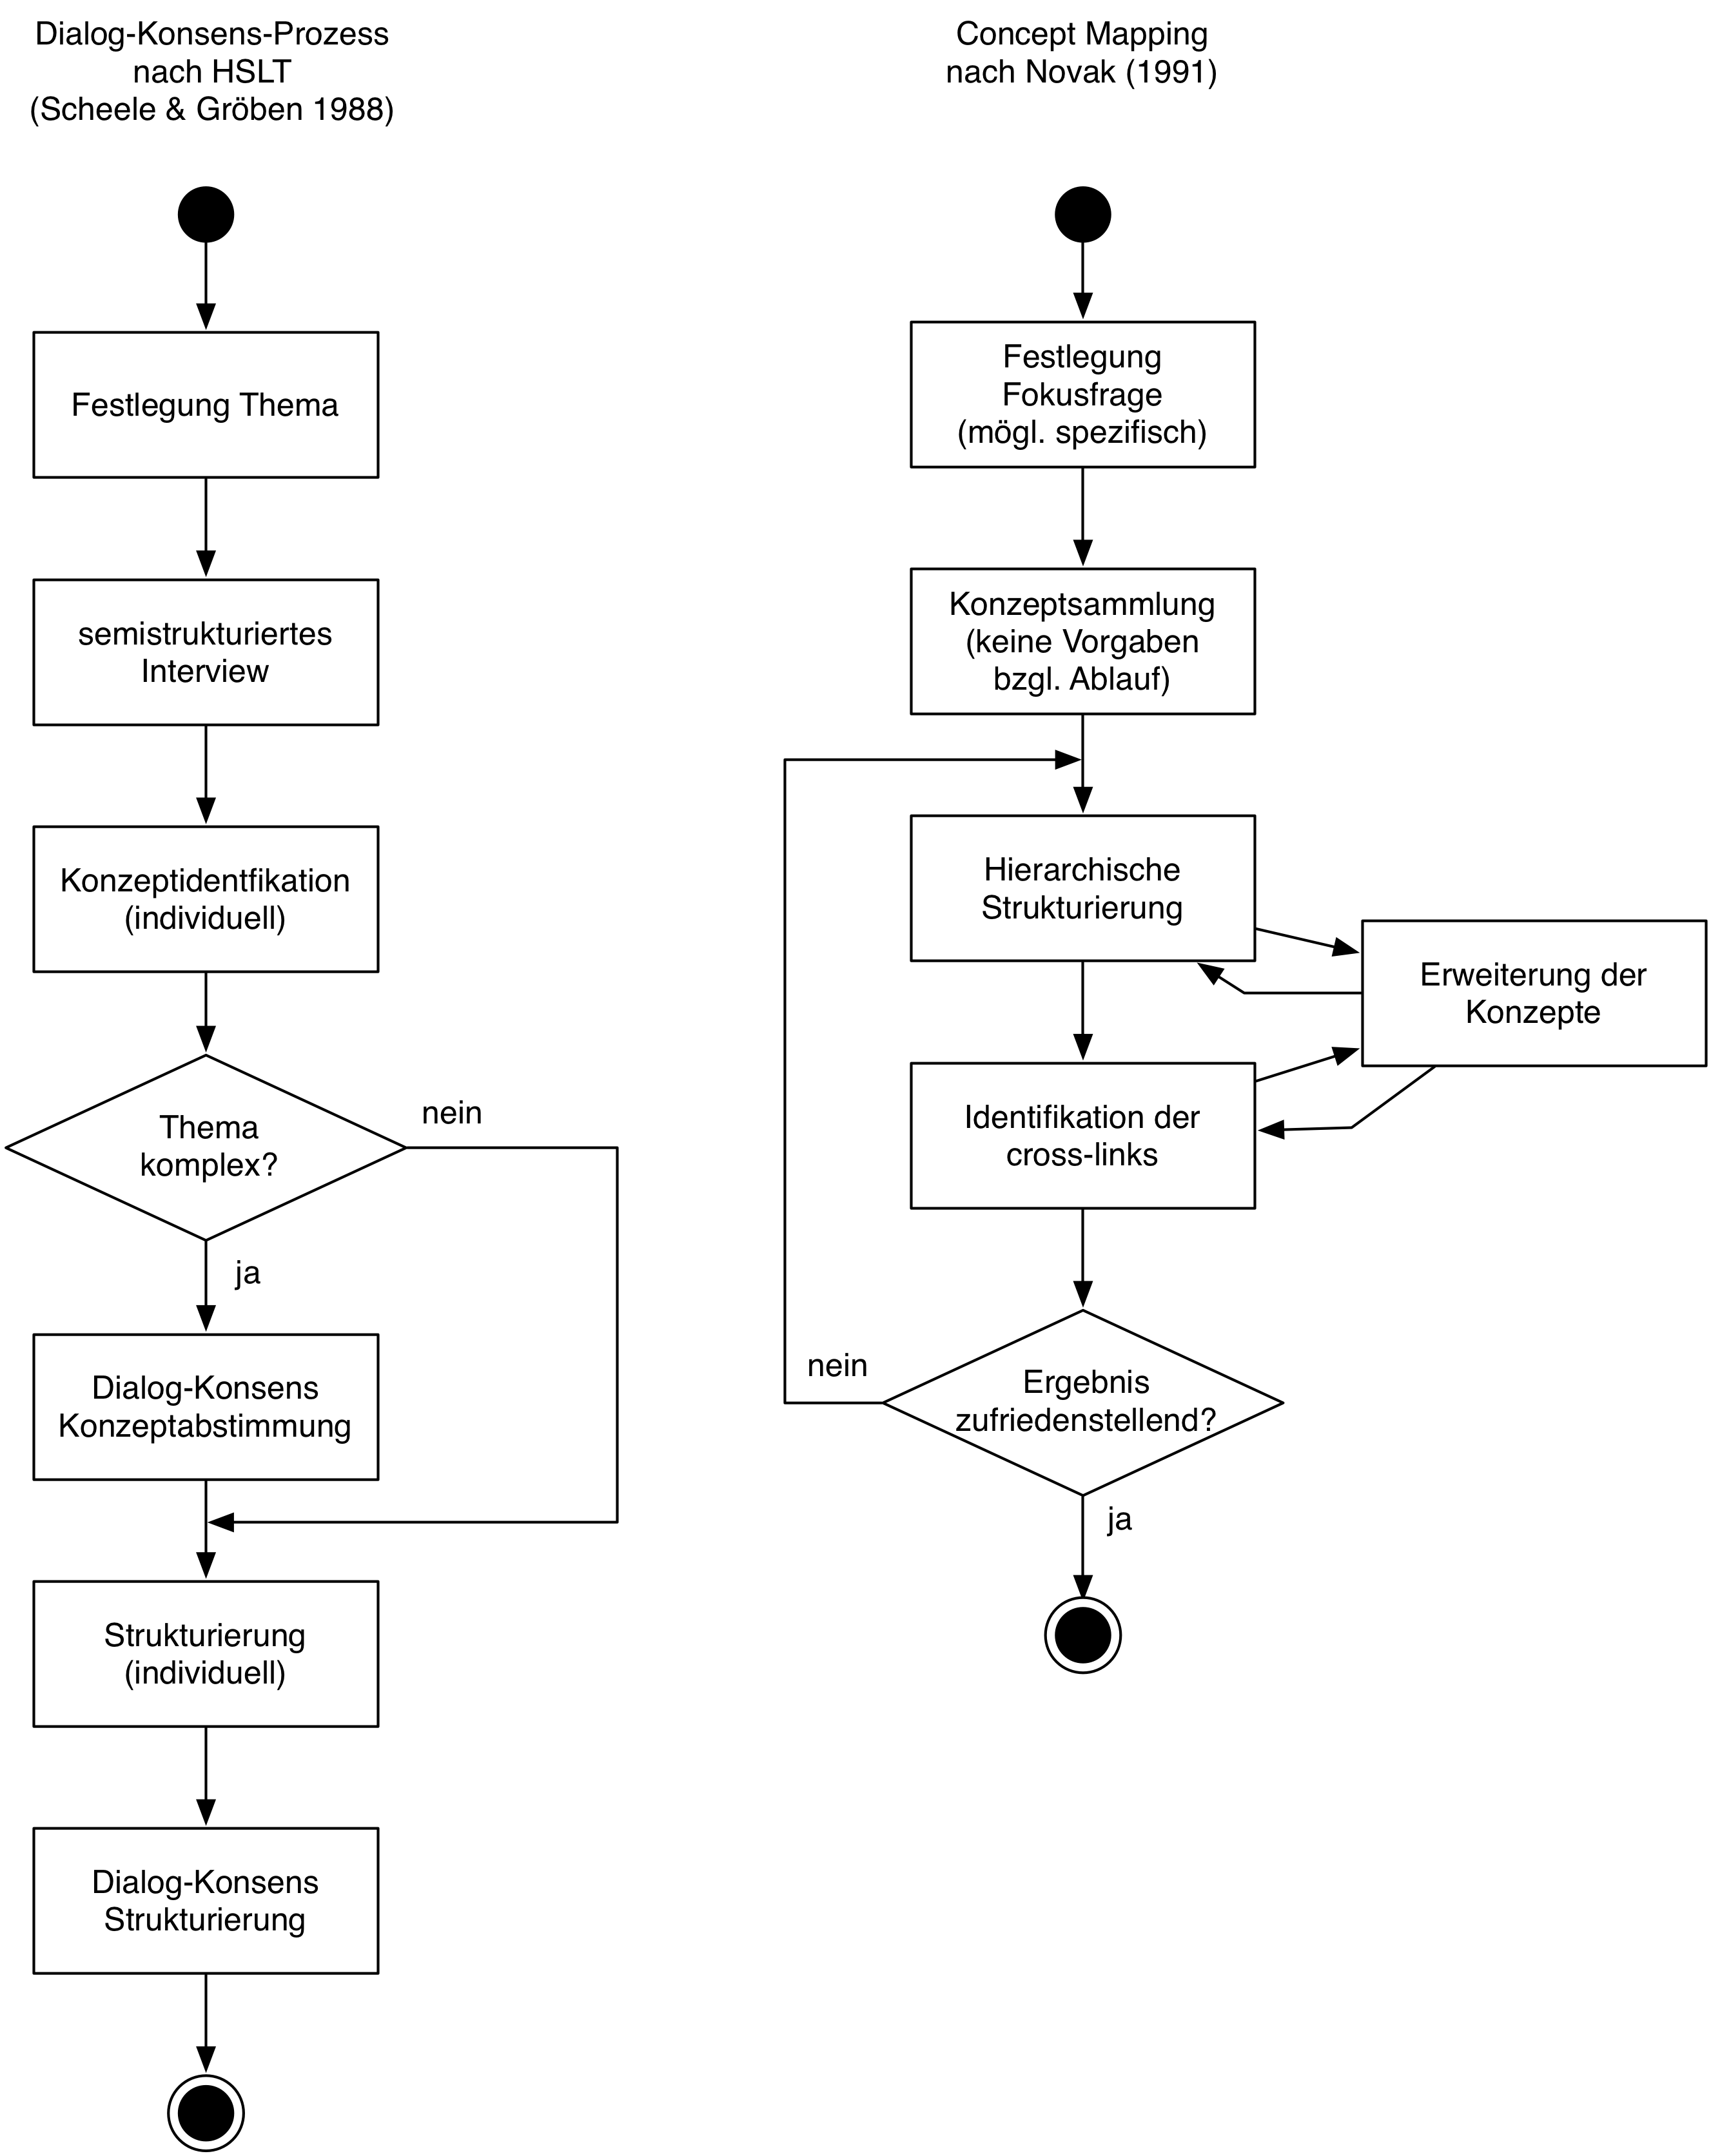
\includegraphics[width=\textwidth]{img/MentaleModelle/slt_cm.png}
	\caption{Externalisierung mentaler Modelle mittels Strukturlegetechniken und Concept Mapping}
	\label{fig:img_MentaleModelle_slt_cm}
\end{figure}

Das „Dialog-Konsens“-Vorgehen nach \citet{Scheele88} ist stark reglementiert und in den einzelnen Schritten mit definierten Methoden bzw. Vorgehensvorschriften hinterlegt. Die im Rahmen von „Concept Mapping“ vorgeschlagene Methode ist hier offener und erscheint damit für die Anwendung im Rahmen von „expliziter Articulation Work“ besser geeignet. Dies liegt am eher informellen Durchführungsrahmen von „expliziter Articulation Work“ begründet, deren Ausgestaltung individuell verschieden ist und zwischen den Beteiligten (im gängigsten Fall implizit) ausgehandelt wird. Ziel ist hier, den Artikulations-Prozess zu unterstützen und nicht, ihn zu formalisieren und in vorgegebene Ablauf-Grenzen zu pressen. 

Auch die zweiphasige Durchführung des Modellierungsprozesses muss unter diesem Gesichtspunkt hinterfragt werden. Die Unterteilung in zwei Phasen erscheint bei der Beschreibung von konzeptionellen Modellen sinnvoll. Begründet liegt dies in der Vielfalt möglicher Strukturierierungsvarianten bei dieser Art von Modellen. Im Gegensatz dazu ist die zweistufige Abhandlung der Externalisierung bei Modellen von Abläufen nur bedingt sinnvoll, da Aktivitäts-Konzepte im Normalfall bereits in deren kausalen Abfolge externalisiert und dann bzw. parallel mit zusätzlichen Konzepten hinterlegt werden. Diese Form von Modellen ist bei der Abstimmung von Arbeit gängig, wird aber weder bei Concept Mapping noch bei Strukturlegetechniken explizit angesprochen. Insofern ist die explizite Durchführung der ersten Phase -- also der Konzeptsammung -- als optional anzusehen. Im Sinne der Methode zur Erstellung von Concept Maps nach /citep{Novak06} werden Konzeptsammlungs-Phasen in den iterativen Modellverfeinerungsprozess eingeflochten, wenn dies in der Situation als notwendig erscheint.

Die einzelnen Schritte, die bei der Anwendung des Werkzeugs zur Anwendung kommen, sind im Einzelnen:
\begin{itemize}
 \item Einschulung
 \item Konzeptsammlung 
 \item Konzeptstrukturierung
 \item Restrukturierung
\end{itemize}

Diese Aufzählung gibt keine Reihenfolge der durchzuführenden Schritte vor. Vielmehr sind die einzelnen Blöcke als Module zu sehen, die je nach Anwendungsfall zu einem beliebigen Zeitpunkt im Externalisierungsprozess (auch mehrfach) zur Anwendung kommen oder auch entfallen können. Im Folgenden wird die Durchführung der einzelnen Schritte kurz umrissen und angegeben, in welchen Situationen deren Einsatz angemessen bzw. notwendig erscheint.

\subsection{Einschulung}

\subsection{Konzeptsammlung}

\subsection{Konzeptstrukturierung}

\subsection{Restrukturierung}
% section vorgehen (end)

\section{Anwendungsszenarien}

Prototypische Zusammenstellungen der Vorgehensblöcke je nach Setting der Abstimmung mentaler Modelle.

\begin{itemize}
 \item Verfeinerung individueller mentaler Modelle (rein indiv.)
 \item Wissenstransfer (1:n)
 \item Abstimmung individueller mentaler Modelle (indiv -> koop.)
 \item Aushandlung individueller mentaler Modelle (von Beginn an koop.)
\end{itemize}




% chapter methodik (end)

% part grundlagen (end)

 
\newpage
\textcolor{white}
.
\textcolor{black}
\newpage

\cleardoublepage

\part{Unterstützung} % (fold)
\label{prt:umsetzung}

%\chapter{Methodik und Anwendungszenarien} % (fold)
\label{cha:methodik}

In diesem Kapitel wird die Methodik vorgestellt, die zur Externalisierung von mentalen Modellen mit dem zu entwickelnden Werkzeug zur Anwendung kommt. Die Inhalte dieses Kapitels bauen auf den Ergebnissen der Kapitel \ref{cha:articulation_work}  und \ref{cha:mentale_modelle} auf. Die Anforderungen, die sich auf der hier vorgestellen Methodik ergeben, werden in Kapitel \ref{cha:anforderungen} identifiziert und in weiterer Folge in einem Werkzeug umgesetzt.

Basierend auf den Schlussfolgerungen, die \citet{Ifenthaler06} hinsichtlich der Eignung der beschriebenen Methoden zur Externalisierung von mentalen Modellen zieht, scheinen jene Ansätze, die auf der Bildung diagrammatischer Modelle basieren besser für die Unterstützung expliziter „Articulation Work“ geeignet zu sein als Methoden, die auf einer rein natürlichsprachlichen Repräsentation aufbauen. Dies liegt vor allem in der höheren Abstraktion begründet, die die externe Repräsentation als interindividuellen Ankerpunkt für Kommunikation besser geeignet macht. Dies deckt sich mit den Aussagen von  \citet{Sarini02}, \citet{Herrmann02}, \citet{Raposo04} oder \citet{Jorgensen04}, die aus Sicht von „Articulation Work“ für die Verwendung von (diagrammatischen) Modellen zur Unterstützung argumentieren.

Betrachtet man nun die beiden Vertreter der auf diagrammatischen Modellen aufbauenden Methoden -- Strukturlegetechniken und Concept Mapping --, so zeigt sich hinsichtlich der Eignung zum Unterstützung von „Articulation Work“ kein eindeutiger Vorteil für eine der beiden Methoden. Vielmehr weisen beide in diesem Kontext Vor- und Nachteile auf. Hier wird deshalb versucht, die Vorteile von Strukturlegetechniken -- im Wesentlichen die Unmittelbarkeit der physischen Repräsentation -- mit jenen von Concept Mapping -- der Flexibilität der Modellierung sowie der Möglichkeit der Unterstützung des Modellierungsprozesses durch Computersysteme -- zu vereinen.

Dabei wird auf das für „Articulation Work“ besser geeignete methodische Vorgehen von „Concept Mapping“ zurückgegriffen, während die Modellierungsumgebung an das Setting von „Strukturlegetechniken“ angepasst wird.

\section{Durchführungsrahmen} % (fold)
\label{sec:durchführungsrahmen}

Der Rahmen, in explizite „Articulation Work“ mit Unterstützung von externalisierten Modellen durchgeführt wird, ist an den Aufbau von Strukturlegetechniken angelehnt. Eine wesentliche Eigenschaft ist hierbei die physische Modellierungsoberfläche, auf der das Modell mittels real vorhandener und unmittelbar manipulierbaren Elementen aufgebaut wird. 

Im Sinne der Abstimmung unterschiedlicher Sichten muss eine kooperative, nicht exklusive Manipulierbarkeit des Modells gewährleistet sein. Das Modell selbst ist -- orientiert an der Offenheit der Repräsentation bei „Concept Mapping“ -- weder in der Art der Elemente noch der Beziehungen eingeschränkt. 

Hinsichtlich des Durchführungsrahmen ist auch die Notwendigkeit des Einsatzes einer Person zu diskutieren, die den Externalisierungsprozess anleitet und steuernd in diesen eingreift. Die Dialog-Konsens-Methode, die im Rahmen von Strukturlegetechniken zur Anwendung kommt, sieht die Rolle eines Untersuchungsleiters vor, der den Ablauf der Externalisierung strukturell anleitet. Inhaltlich hat der Untersuchungsleiter jedoch keine neutrale Rolle inne, sondern tritt im Rahmen des Dialog-Konsens-Prozesses in Interaktion mit der externalisierenden Person. Ziel des Untersuchungsleiters ist es, das mentale Modell der externalisierenden Person zu erschließen und zu verstehen. In kooperativen Situationen (die von der Dialog-Konsens-Methode nach \citep{Scheele88} nicht explizit berücksichtigt werden), wo gegenseitiges Verständnis erreicht werden muss, wechselt demnach die Rolle des Untersuchungsleiters inhaltlich gesehen dynamisch. 

Aus Sicht der Prozesssteuerung kann zu diesem Zeitpunkt nicht entschieden werden, ob ein Untersuchungsleiter benötigt wird oder nicht. Bei Strukturlegetechniken beschränkt sich dessen Aufgabe auf die Sicherstellung der Fokussierung der beteiligten Personen auf die jeweilige Aufgabe. Im Rahmen der Concept Mapping Methode ist ein intervenierender Untersuchungsleiter nicht vorgesehen. Im Rahmen der empirischen Erhebung (siehe Kapitel XY) wird untersucht, ob diese Rolle bei der Anwendung des hier vorgeschlagenen Werkzeugs notwendig ist oder unbesetzt bleiben kann. 

% subsection durchführungsrahmen (end)

\section{Vorgehen} % (fold)
\label{sub:vorgehen}

Sowohl im Bereich der Strukturlegetechniken als auch im „Concept Mapping“ wird vorgeschlagen, den initialen Modellierungsprozess in zwei Phasen -- Konzeptsammlung und Konzeptstrukturierung -- zu teilen und in der Folge das Modell iterativ solange zu verändern bzw. zu erweitern, bis alle Beteiligten mit der Lösung zufrieden sind (im Bereich der Strukturlegetechniken wird die als „Dialog-Konsens“ bezeichnet, im „Concept Mapping“ spricht man von „Revisions“ des Modells, die erstellt werden müssen). Beide Abläufe sind abstrahiert in Abbildung \ref{fig:img_MentaleModelle_slt_cm} dargestellt.

\begin{figure}[htbp]
	\centering
		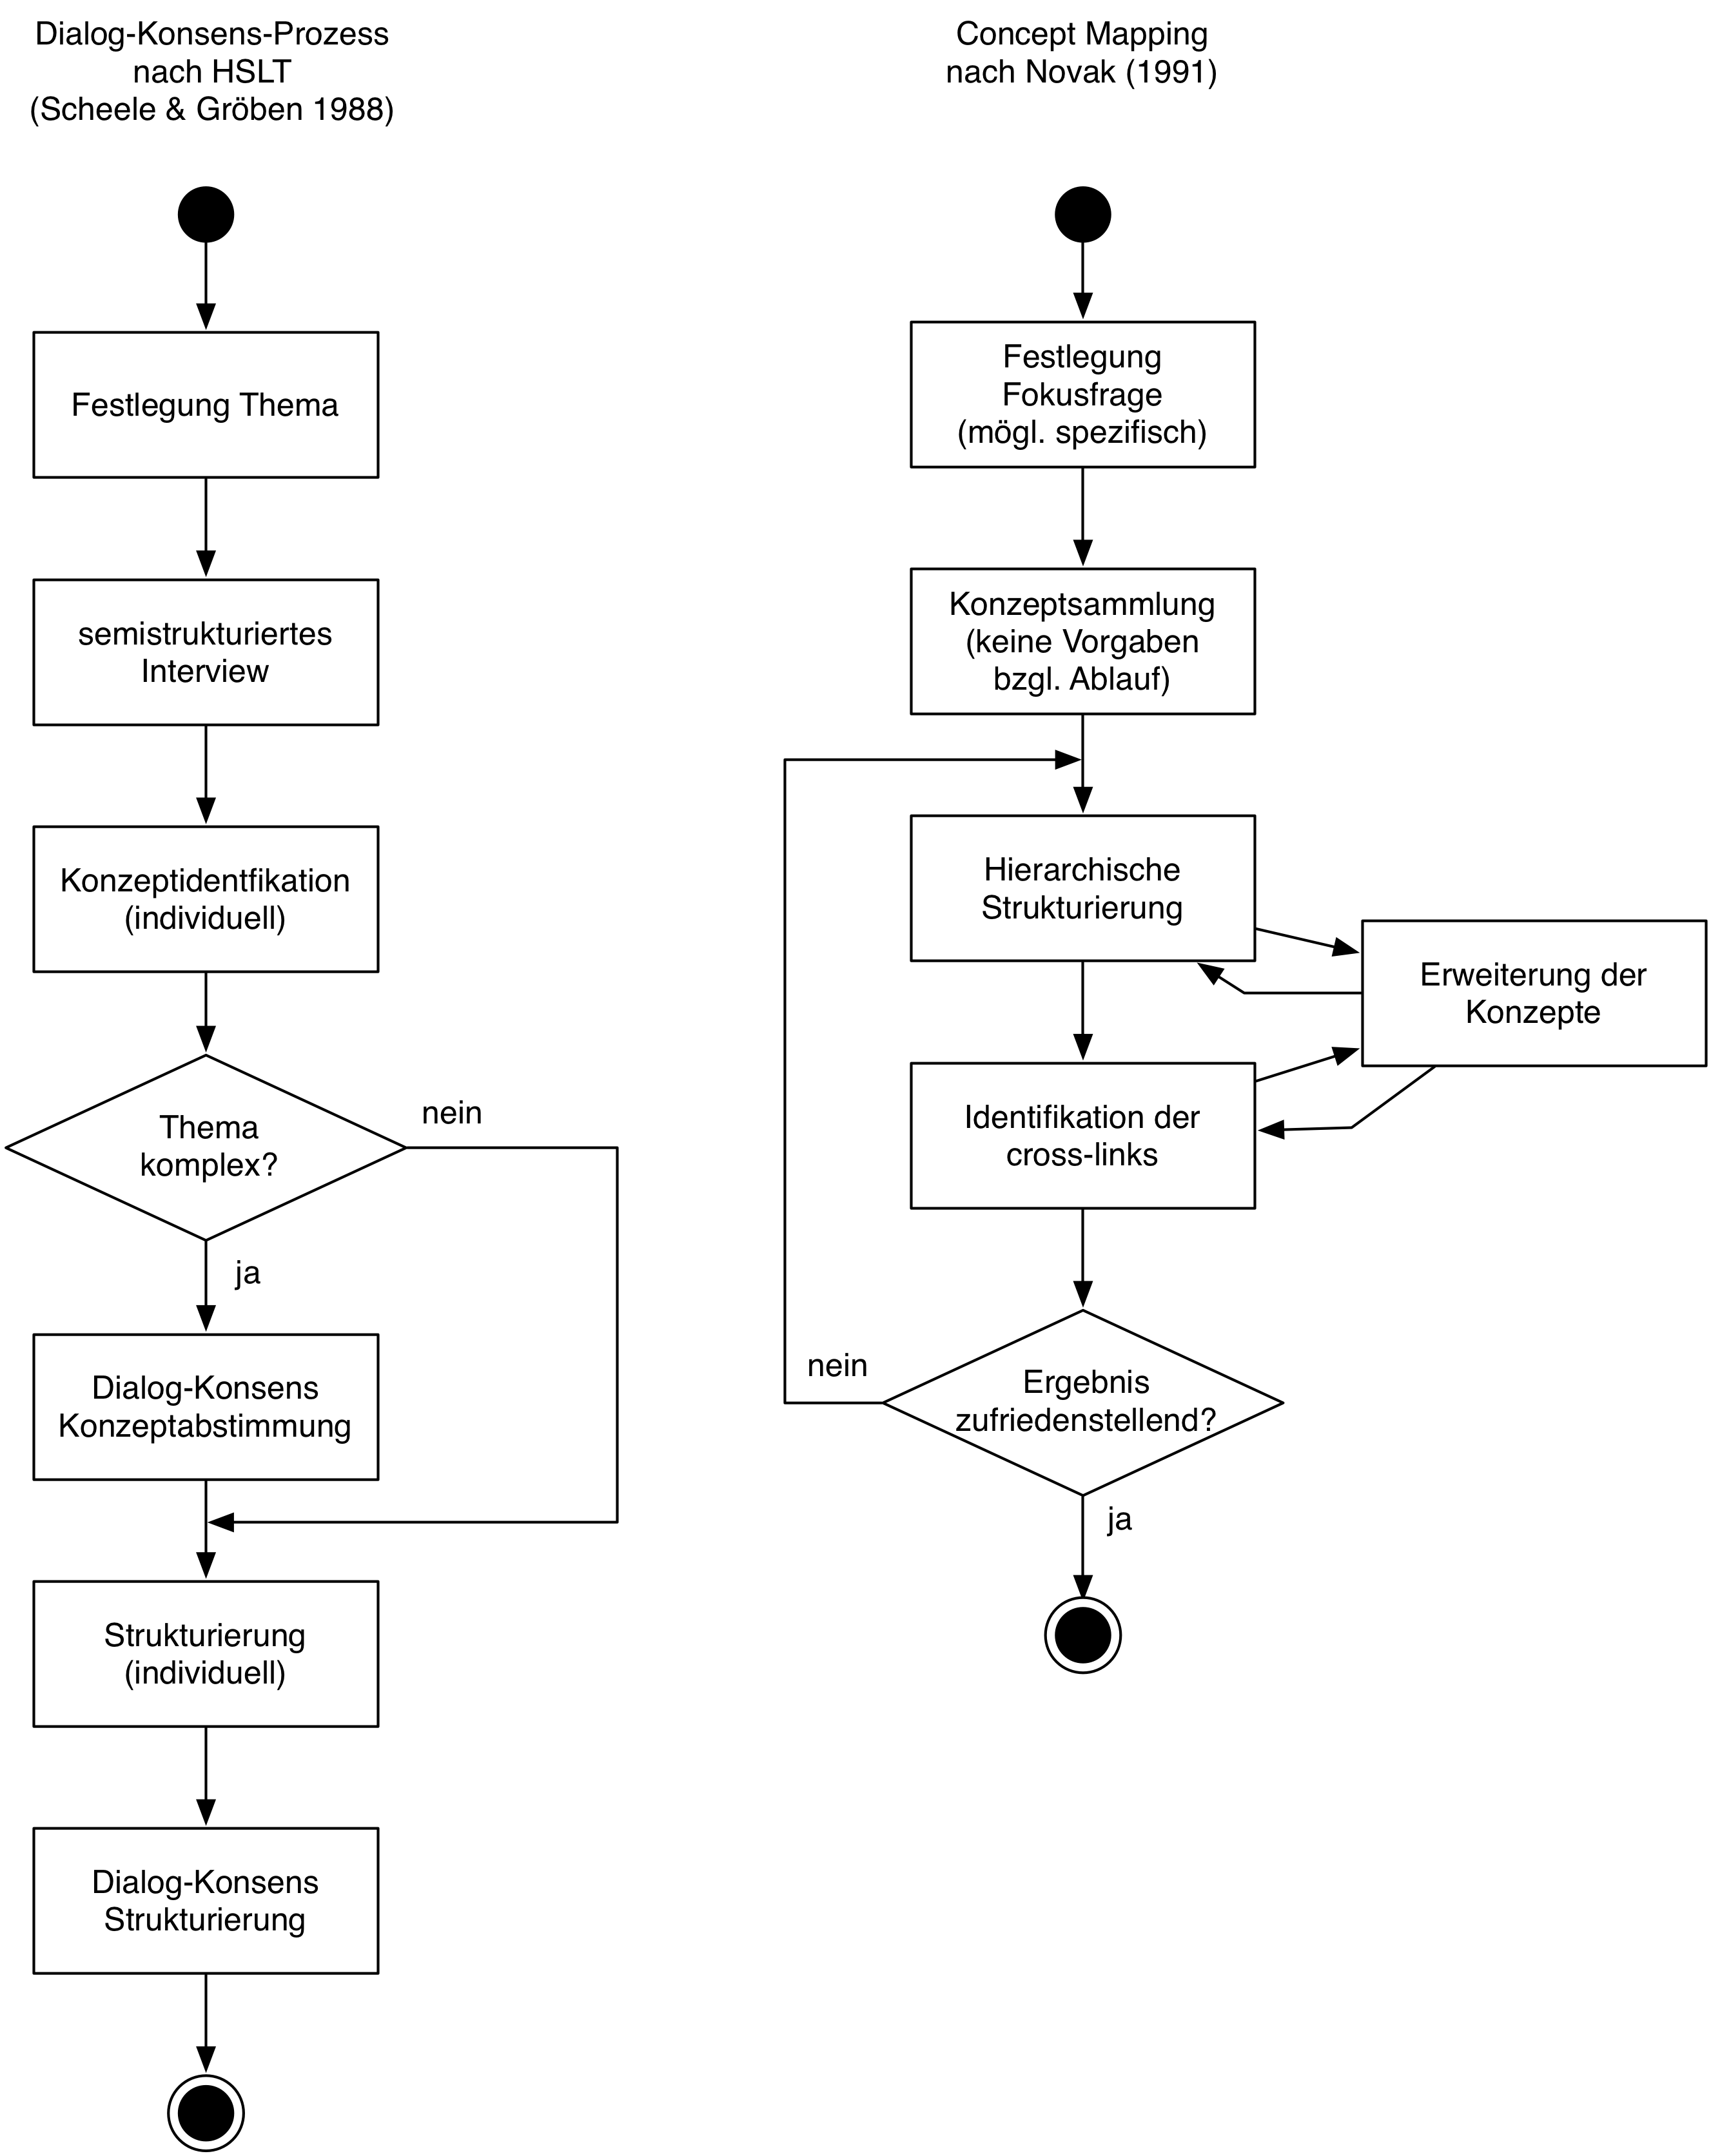
\includegraphics[width=\textwidth]{img/MentaleModelle/slt_cm.png}
	\caption{Externalisierung mentaler Modelle mittels Strukturlegetechniken und Concept Mapping}
	\label{fig:img_MentaleModelle_slt_cm}
\end{figure}

Das „Dialog-Konsens“-Vorgehen nach \citet{Scheele88} ist stark reglementiert und in den einzelnen Schritten mit definierten Methoden bzw. Vorgehensvorschriften hinterlegt. Die im Rahmen von „Concept Mapping“ vorgeschlagene Methode ist hier offener und erscheint damit für die Anwendung im Rahmen von „expliziter Articulation Work“ besser geeignet. Dies liegt am eher informellen Durchführungsrahmen von „expliziter Articulation Work“ begründet, deren Ausgestaltung individuell verschieden ist und zwischen den Beteiligten (im gängigsten Fall implizit) ausgehandelt wird. Ziel ist hier, den Artikulations-Prozess zu unterstützen und nicht, ihn zu formalisieren und in vorgegebene Ablauf-Grenzen zu pressen. 

Auch die zweiphasige Durchführung des Modellierungsprozesses muss unter diesem Gesichtspunkt hinterfragt werden. Die Unterteilung in zwei Phasen erscheint bei der Beschreibung von konzeptionellen Modellen sinnvoll. Begründet liegt dies in der Vielfalt möglicher Strukturierierungsvarianten bei dieser Art von Modellen. Im Gegensatz dazu ist die zweistufige Abhandlung der Externalisierung bei Modellen von Abläufen nur bedingt sinnvoll, da Aktivitäts-Konzepte im Normalfall bereits in deren kausalen Abfolge externalisiert und dann bzw. parallel mit zusätzlichen Konzepten hinterlegt werden. Diese Form von Modellen ist bei der Abstimmung von Arbeit gängig, wird aber weder bei Concept Mapping noch bei Strukturlegetechniken explizit angesprochen. Insofern ist die explizite Durchführung der ersten Phase -- also der Konzeptsammung -- als optional anzusehen. Im Sinne der Methode zur Erstellung von Concept Maps nach /citep{Novak06} werden Konzeptsammlungs-Phasen in den iterativen Modellverfeinerungsprozess eingeflochten, wenn dies in der Situation als notwendig erscheint.

Die einzelnen Schritte, die bei der Anwendung des Werkzeugs zur Anwendung kommen, sind im Einzelnen:
\begin{itemize}
 \item Einschulung
 \item Konzeptsammlung 
 \item Konzeptstrukturierung
 \item Restrukturierung
\end{itemize}

Diese Aufzählung gibt keine Reihenfolge der durchzuführenden Schritte vor. Vielmehr sind die einzelnen Blöcke als Module zu sehen, die je nach Anwendungsfall zu einem beliebigen Zeitpunkt im Externalisierungsprozess (auch mehrfach) zur Anwendung kommen oder auch entfallen können. Im Folgenden wird die Durchführung der einzelnen Schritte kurz umrissen und angegeben, in welchen Situationen deren Einsatz angemessen bzw. notwendig erscheint.

\subsection{Einschulung}

\subsection{Konzeptsammlung}

\subsection{Konzeptstrukturierung}

\subsection{Restrukturierung}
% section vorgehen (end)

\section{Anwendungsszenarien}

Prototypische Zusammenstellungen der Vorgehensblöcke je nach Setting der Abstimmung mentaler Modelle.

\begin{itemize}
 \item Verfeinerung individueller mentaler Modelle (rein indiv.)
 \item Wissenstransfer (1:n)
 \item Abstimmung individueller mentaler Modelle (indiv -> koop.)
 \item Aushandlung individueller mentaler Modelle (von Beginn an koop.)
\end{itemize}




% chapter methodik (end)
%\input{Design}

%\chapter{Implementierung – Überblick} % (fold)
\label{cha:implementierung_Überblick}

Wie im Kapitel "Design" gefordert, wurde zur Umsetzung des Werkzeugs ein "Tangible Tabletop Interface" verwendet. Tabletop Interface zeichnen sich im Generellen dadurch aus, dass im Gegensatz zu handelsüblichen Rechnern nicht nur die Software sondern auch die Hardware applikationsspezifisch ist und nicht generisch eingesetzt werden kann. Die Hardware bildet dabei einen Teil oder die gesamte Benutzungsschnittstelle ab. Im speziellen Fall eines "Tangible Tabletop Interfaces" basiert der Benutzerinteraktion auf der Verwendung physischer Bausteine ("Tokens"), die auf der physischen Oberfläche des Interfaces manipuliert werden. Dieses Paradigma wird ergänzt von Tabletop Interfaces, die die Benutzerinteraktion ausschließlich auf Gesten bzw. Berührungen der Oberfläche abbilden (horizontal verbaute "Touch-" bzw. "Multi-Touch-Displays").

\section{Grundlegende \& verwandte Arbeiten} % (fold)
\label{sec:grundlegende_&_verwandte_arbeiten}

REFs!!! Die Entwicklung von Tabletop Interfaces begann Mitte der 1990er-Jahren mit den Arbeiten von Ishii \& Ullmer. Auch die erste Anwendung, die sich mit Modellierungs-Ansätzen mit Hilfe von Tabletop Interfaces konzentriert, stammt aus dieser Zeit. Mit dem fortschreiten der technologischen Entwicklung ist heute ein Status erreicht, in dem mit Hilfe generischer Identifikations-Frameworks schnell und ohne großen Aufwand Applikationen mit "tangiblen" Inputkanälen erstellt werden können. Zur Zeit noch im Prototypenstatus befinden sich Ansätze, die sich mit generischen Möglichkeiten des tangiblen Informationsoutputs beschäftigt. Der Rückkanal vom Rechner zum Benutzer wird heute zumeist mit der Projektion von Inhalten auf die Arbeitsoberfläche umgesetzt.

In den folgenden Abschnitten wird die historische Entwicklung von Tabletop Interfaces sowie der aktuelle Stand der Entwicklung im Anwendungsbereich dieser Arbeit betrachtet. Es werden dabei die grundlegenden Konzepte und Eigenschaften der jeweiligen Arbeiten betrachtet und das Potential hinsichtlich der Umsetzung von in Kapitel XY identifizierten Anforderungen an das hier entwickelte Werkzeug betrachtet. 

\subsection{Tangible Interfaces} % (fold)
\label{sub:tangible_interfaces}

Der Begriff der Tangible bzw. Graspable Interfaces – also der "berührbaren" oder "begreifbaren" Benutzungsschnittstellen — stammt aus der Mitte der neunziger Jahre des zwanzigsten Jahrhunderts. \citet{Fitzmaurice95} werden im Allgemeinen als die ersten betrachtet, die den Begriff des "Graspable User Interfaces" prägen und damit die Manipulierbarkeit digitaler Information durch physische Mittel beschreiben. \citet{Fitzmaurice96} präzisiert später den Begriff durch die Abgrenzung zwischen (herkömmlichen, maus-, tastatur- und bildschirmbasierenden) zeitlich gemultiplexten Schnittstellen, bei denen der Informationsaustausch zwischen Benutzer und System über einen Kanal zeitlich hintereinander erfolgt und den (neuartigen, berührbaren) räumlich gemultiplexten Schnittstellen, bei denen mehrere Kanäle gleichzeitig zur Interaktion zwischen Benutzer und System verwendet werden können. 

Der Begriff des "Tangible User Interfaces" wurde kurz danach bzw. parallel dazu von \citet{Ishii97} eingeführt. \citeauthor{Ishii97} verfolgen dabei bei der Definition den umgekehrten Weg und sprechen von einer "Augmentation der realen Welt durch eine Kopplung von digitaler Information and physische Objekte"\footnote{\emph{“augment the real physical world by coupling digital information to everyday physical objects and environments”}\citep{Ishii97}}. 

% subsection tangible_interfaces (end)

\subsection{Historische Entwicklung von Tabletop Interfaces} % (fold)
\label{sub:historische_entwicklung_von_tabletop_interfaces}

\paragraph{Sensetable} % (fold)
\label{par:sensetable}
Der Sensetable \citep{Patten01}
% paragraph sensetable (end)

\paragraph{BUILD-IT} % (fold)
\label{par:build_it}
\citep{Fjeld01}
% paragraph build_it (end)
% subsection historische_entwicklung_von_tabletop_interfaces (end)

\subsection{Tangible Interfaces zur Modellbildung} % (fold)
\label{sub:tangible_interfaces_zur_modellbildung}

% subsection tangible_interfaces_zur_modellbildung (end)

\subsection{Aktuelle verwandte Ansätze} % (fold)
\label{sub:aktuelle_verwandte_ansätze}

% subsection aktuelle_verwandte_ansätze (end)
\begin{itemize}
	\item Historische Entwicklung von Tabletop Interfaces
	\begin{itemize}
		\item Sensetable
		\item Morten Fjeld
		\item ReacTable
		\item Eva Hornecker
	\end{itemize}
	\item Historische Entwicklung von Tangible Interfaces zur Modellbildung
	\begin{itemize}
		\item Sensetable Modeling Application
		\item Designer's Outpost (Klemmer)
	\end{itemize}
	\item Aktuelle verwandte Ansätze
	\begin{itemize}
		\item Antle (TEI Mail-Pointer)
		\item Sun (TEI Demo)
	\end{itemize}
\end{itemize}


% section grundlegende_&_verwandte_arbeiten (end)

% chapter implementierung_Überblick (end)
\chapter{Input \& Interpretation} % (fold)
\label{cha:input_&_interpretation}
In diesem Kapitel wird jener Teil des Werkzeuges beschrieben, in dem die Interaktion der der Benutzer mit dem Werkzeug erfasst und interpretiert wird. Der erste Abschnitt behandelt grundlegende Möglichkeiten zur Erfassung der Benutzerinteraktion auf tisch-basierten Benutzungsschnittstellen und endet mit der Identifikation der im konkreten Anwendungsfalls geeignetsten Technologie. Diese wird durch die Beschreibung von dafür verfügbaren Frameworks konkretisiert, was letzendlich in der Entscheidung für ein konkretes Produkt mündet.

Basierend auf dieser Entscheidung wird in den folgenden beiden Abschnitten auf das Design der Hard- und Softwarekomponenten eingegangen, die unmittelbar der Eingabe von Information durch Benutzer dienen. Der Ausgabeaspekt wird hier bewusst ausgeklammert und im nächsten Kapitel beschrieben. Dieses Kapitel endet mit eine Beschreibung der Interpretationsroutinen, die aus den durch das Framework gelieferten Rohdaten höherwertige, anwendungsspezifische Information extrahieren und diese den nachgeordneten Software-Modulen zur Verfügung stellen.

\section{Möglichkeiten zur Erfassung von Benutzerinteraktion} % (fold)
\label{sec:möglichkeiten_zur_erfassung_von_benutzerinteraktion}

Im Gegensatz zu Systemen mit dezidierten Eingabegeräten (wie Tastatur oder Maus) ist die Informationseingabe bei Tangible Interfaces unmittelbar an physische Tokens gebunden, die unabhängig voneinander und gegebenenfalls auch simultan manipuliert werden können. Diese Manipulation wird von einer vorhandenen Infrastruktur erfasst und im Sinne von Eingabedaten interpretiert. Der wesentliche Unterschied zu dezidierten Eingabegeräten besteht darin, dass die Manipulation des physischen Artefakts selbst für den Benutzer bedeutungstragend ist und nicht nur dem Zweck einer Zustandsänderung des digitalen Informationsraums dient. Dies impliziert, dass der Zustand der verwendeten Tokens bzw. der aktuelle Wert deren relevanten Parameter (z.B. Position, Rotation, Form, ...) erfasst werden kann, ohne die Bedeutung der Tokens noch deren Manipulierbarkeit in der realen Welt zu beeinflussen. Je nach Anwendungsfall kommen dafür mehrere Unterschiedliche technologische Ansätze in Frage. Die Beurteilungskriterien die dabei zu berücksichtigen sind, liegen nicht nur in den zu erhebenden Parametern begründet sondern umfassen auch die notwendige Erfassungsrate des Zustandes der Tokens sowie die Anzahl der simultan zu erfassenden Tokens bzw. Eigenschaften.

Im konkreten System muss - wie in Kapitel XY beschrieben - die planare Position von mehreren Tokens in Echtzeit (d.h. mehrmals pro Sekunde mit für den Benutzer nicht wahrnehmbaren Verzögerungen) erfasst werden. Neben der Position ist noch die Rotation eines Tokens als Raumparameter von Interesse. Bezüglich des Zustands eines Tokens muss erfasst werden können, ob es geöffnet oder geschlossen ist und ob es eingebettete Objekte enthält oder nicht. Mit diesen Anforderungen wird in den folgenden Unterabschnitten ein technologischer Ansatz zur Umsetzung der Interaktionserkennung ausgewählt.

\subsection{In Frage kommende technologische Ansätze} % (fold)
\label{sub:potentielle_technologische_ansätze}
Bei der Auswahl möglicher technologischer Ansätze zur Erfassung der Benutzerinteraktion müssen die zu erfassenden Parameter unterschiedlich behandelt werden. Konkret werden hier Ansätze zur Erfassung der Raumparameter (Position, Rotation) und Ansätze die Zustandsänderungen des Tokens erfassbar machen unterschieden. 

\subsubsection{Raumparameter} % (fold)
\label{ssub:raumparameter}
\index{Positionsbestimmung} 
Zur Erfassung von Raumparametern von Tokens bieten sich mehrere technologische Ansätze an. In Frage kommen für das konkrete - tisch-basierte System - nur Technologien, die eine Erfassung dieser Parameter mit einer Genauigkeit im Zentimeter- bis Millimeter-Bereich ermöglichen, da eine niedrigere Raumauflösung zu zu großen Ungenauigkeiten in der Positionsbestimmung führen würden, die einen Einsatz für das hier vorgestellte Werkzeug nicht erlauben würden. Im Folgenden werden die in Frage kommenden Technologien in ihren Grundzügen beschrieben und hinsichtlich ihrer Eignung für das konkrete System bewertet.

\paragraph{Optisch} % (fold)
\label{par:optisch}
\index{Positionsbestimmung!optisch} 
\index{Barcode} 

Optische Positionsbestimmung erfolgt immer mit Hilfe von Kamera-Systemen und Methoden der digitalen Bildverarbeitung. Die Kamera erfasst dabei die zu identifizierenden Tokens, dass resultierende Bild wird mit in Software umgesetzten Algorithmen ausgewertet, wodurch zumindest Identität und Position, zumeist aber auch weitere Raumparameter (wie Rotation) aller im Kamerabild befindlichen Tokens ermittelt werden können. Die Erkennung ist dabei auf den Erfassungsbereich der Kamera beschränkt. Neben diesem Einflussfaktor bestimmen zudem die Auflösung der Kamera sowie die Größe der Tokens die letztendlich erfassbare Fläche. Optische Systeme sind generell bei schlechten oder wechselnden Lichtverhältnissen eher fehleranfällig und nicht robust gegen Verdeckungen von Tokens (etwa durch Gliedmaßen oder andere Tokens).

Hinsichtlich des Identifikationsansatzes können zwei Arten von Systemen unterschieden werden. \emph{Codebasierte} Systeme verwenden zur Identifikation eines Tokens einen von der Kamera erfassbaren Code (etwa einen "Barcode"), der eindeutig einem Token zugeordnet werden kann. \emph{Featurebasierte} Systeme identifizieren ein Token aufgrund seiner äußeren Eigenschaften, zumeist über dessen Form (Schattenriss). Letztere bieten den Vorteil, dass ein Token nicht durch das Anbringen eines zusätzlichen Codes optisch verändert werden muss. Der größte Nachteil besteht in der Eigenschaft, dass nur Token mit unterschiedlichen Formen eindeutig identifiziert werden können. Die eindeutige Identifikation von mehreren Tokens einer Bauart ist bei featurebasierten Systemen nicht möglich. Codebasierte Systeme verwenden zumeist nicht herkömmliche Barcodes sondern robustere Systeme, bei denen eine Erkennung auch unter widrigen Beleuchtungsbedingungen oder niedrigen Bildauflösungen möglich ist und die zum Teil auch die Extraktion zusätzliche Information über weitere Raumparameter (wie Rotation, teilweise auch Parameter der dritten Dimension wie Neigung oder Entfernung) ermöglichen. 

Codebasierte Systeme können hinsichtlich der Art der Codierung der Indentitätsinformation wiederum in zwei Klassen unterschieden werden. Eine Gruppe von Ansätzen integriert die eigentliche Nutzinformation, also im Wesentlichen die tokenspezifische Identifikationsnummer, direkt in den Code und ermöglicht so ein direktes Auslesen der Information (z.B. bei QRCode (REF)). Die zweite Gruppe verwendet eine indirekte Zuordnung zwischen Token-ID und Code. Bei derartigen Ansätzen muss die Identität eines Tokens in einem Zwischenschritt über eine Mapping-Tabelle abgebildet werden, im Gegenzug ist die Ausgestaltung des Codes flexibler, im Allgemeinen kann dabei eine höhere Robustheit bei der Erkennung erreicht werden (z.B. ARToolkit (REF)).

% paragraph optisch (end)

\paragraph{Kapazitiv} % (fold)
\label{par:kapazitiv}
\index{Positionsbestimmung!kapazitiv}  

Kapazitive Ansätze basieren auf der Änderung der Kapazität von Leiterbahnen, die durch deren Berührung mit leitfähigem Material verursacht wird. Ursprünglich wurde die Technologie zur Umsetzung von berührungssensitiven Oberflächen entwickelt, kann jedoch auch zum Tracking von Tokens verwendet werden. Im Gegensatz zu druckempfindlichen Oberflächen (klassischen "Touchscreens") ist keine Druckausübung zur Erkennung notwendig, es können außerdem auch mehrere Tokens (bzw. Finger) gleichzeitig erkannt werden.

Technologisch bedingt müssen bei kapazitiven Ansätzen alle zu identifizierenden Objekte die Oberfläche des Systems berühren. In dieser Oberfläche ist ein Metallgitter eingebettet, zwischen dessen Adern eine elektrische Kapazität gemessen werden kann. Diese Kapazität verändert sich, sobald diese Adern berührt werden (wobei die Token in einen entsprechend geeigneten Material ausgeführt sein müssen). Durch die lokale Änderung der Kapazität kann die Position einer Berührung festgestellt werden. Die Genauigkeit ist dabei durch die Rasterweite des Metallgitters eingeschränkt. Der größte Nachteil eines kapazitiven Ansatzes ist in diesem Kontext aber, dass die Identität eine Tokens nicht direkt festgestellt werden kann (die Kapazitätsänderung ist für alle Token identisch). Zudem ist die Extraktion weiterer Raumparameter (wie Rotation) nicht bzw. nur mit zusätzlichen Aufwand möglich. Die Vorteile von kapazitiven Systemen liegen in der hohen Robustheit der Erkennung auch bei widrigen Umgebungseinflüssen (Lichtverhältnisse, Schmutz) sowie der prinzipiell beliebig großen und beliebig geformten Oberfläche, die zur Erkennung verwendet werden kann.

Kapazitive Systeme eignen sich also zur Positionsbestimmung, nicht aber zur Identifikation von Tokens. Dies macht sie für den konkreten Anwendungsfall nur in Kombination mit einer anderen Technologie geeignet. 

% paragraph kapazitiv (end)

\paragraph{Elektromagnetisch} % (fold)
\label{par:elektromagnetisch}
\index{Positionsbestimmung!elektromagnetisch} 
\index{RFID}
 
Die Ausstattung von Tokens mit elektromagnetisch erfassbaren Einheiten (z.B. RFID-Chips) ermöglicht ebenfalls die Erfassung von Raumparametern. Vorrangig eignet sich diese Technologie jedoch zur Identifikation von Tokens, die Positionsbestimmung kann nur mit erheblichem technischen Aufwand durchgeführt werden.

RFID-Chips (als Beispiel für einen elektromagnetischen Ansatz) sind passive Bauteile, die bei Energieversorgung durch ein elektrisches Feld aktiv werden und ihrerseits eine eindeutige Identifikationsnummer senden (im einfachsten Fall, komplexere Varianten sind möglich, werden hier aber nicht betrachtet). Historisch stammt die Technologie aus der Logistik und Warenwirtschaft und dient der Identifikation von Gütern und nicht der exakten Positionsbestimmung. Diese ist somit auch nur mittels erweiterter Infrastruktur möglich. Zum Auslesen eines RFID-Chips wird ein Lesegerät mit Antenne benötigt. Aus der Feldstärke, mit der diese Antenne die Antwort des Chips empfängt, kann auf die Entfernung des Chips von der Antenne geschlossen werden. Durch Kreuzpeilung mit mindestens zwei Antennen, deren Position bekannt ist, kann somit auf die ungefähre Position des Chips (und damit des Tokens, in das dieser eingebaut ist) geschlossen werden. Durch den Einsatz von "Antennenarrays" (matrixförmig angeordneten Antennen) mit geringer Reichweite ist so eine verhältnismäßig exakte (Größenordnung einige cm) Positionsbestimmung möglich. Die Feststellung der Ausrichtung eines Tokens (Rotation) ist auf diesem Wege allerdings nicht möglich. Die Identifikation eines Tokens ist jedoch unabhängig von Sichtkontakt und unmittelbarer Berührung und somit äußerst robust gegen Umgebungseinflüsse.

Elektromagnetische Systeme eignen sich wegen des hohen technischen Aufwandes bei gleichzeitig beschränkter Genauigkeit nur bedingt zur Feststellung von Raumparametern. Durch die Ausrichtung auf Extraktion der Identitätsinformation ist der Ansatz jedoch gut zur Kombination mit anderen Technologien wie kapazitiven Ansätzen geeignet, die ihre Stärken in der Bestimmung der Raumparameter haben.
 
% paragraph elektromagnetisch (end)

\paragraph{Akustisch} % (fold)
\label{par:akustisch}
\index{Positionsbestimmung!akustisch} 
\index{Ultraschall} 

Akustische Ansätze zur Positionsbestimmung basieren im Generellen auf der Laufzeitmessung von Ultraschallwellen im Raum. Mit entsprechender Infrastruktur ist damit in einem begrenzten Bereich ein hochexakte Feststellung der Raumparameter in drei Dimensionen (Genauigkeit im mm-Berich) sowie die Identifikation von Tokens möglich.

Ultraschallbasierte Techniken zur Positionsbestimmung basieren auf dem Einsatz von Bakensendern an bekannten Positionen. Diese Sender werden zumeist an der Zimmerdecke montiert und senden periodisch einen Ultraschallimpuls aus. Dieser Impuls wird von den Tokens (die in diesem Fall aktive Bauteile mit Stromversorgung sind) empfangen, die daraufhin einen sie identifizierenden Impuls zurücksenden. Aus der Laufzeit zwischen Absetzen des Sendeimpuls und Empfangen des Antwortimpulses bei verschiedenen Baken lässt sich so die Position des Tokens im Raum feststellen. Problematisch ist hierbei jedoch die durch den auf sequentieller Zeitmessung basierenden Ansatz beschränkte Anzahl von verfolgbaren Tokens, wenn Echtzeit-Ansprüche gestellt werden. Zudem ist der Ansatz nicht robust gegen (akustisch) verdeckte Tokens. Eine Anfälligkeit gegenüber anderen Störeinflüssen besteht nicht. 

Für die Feststellung von Raumparametern sind ultraschall-basierte Systeme generell ausgezeichnet geeignet. Auch die Identifikation von Tokens ist prinzipiell möglich. Bei der Bewertung hinsichtlich des Einsatzes für tisch-basierte Systeme ist jedoch zu bedenken, dass eine drei-dimensionale Positionierung nicht zu den allgemeinen Anforderungen zählt und nur in speziellen Anwendungsfällen sinnvoll sein kann. Zudem kann die Notwendigkeit von stromversorgten Tokens einen Nachteil bzw. ein Hindernis beim Einsatz darstellen.

% paragraph akustisch (end)

\paragraph{Bewertung} % (fold)
\label{par:bewertung}

Im konkreten Anwendungsfall ist die Feststellung der Identität sowie der planaren Position und Rotation von mehreren Tokens in hoher Genauigkeit sowie in Echtzeit gefordert. Aus oben genannten Gründen sind kapazitive und elektromagnetische Systeme im Einzeleinsatz nur bedingt geeignet. Akustische Systeme erscheinen für den Anwendungsfall als zu aufwändig und unflexibel und stoßen außerdem bei der Anzahl der simultan zu verfolgenden Tokens an ihre Grenzen.

Die Kombination von kapazitiven und elektromagnetischen Systemen ist grundsätzlich eine Möglichkeit, die in Betracht gezogen werden könnte. Auch optische Systeme genügen den Anforderungen und kommen damit in Frage. Der kombinierte Ansatz ist im Vergleich mit optischen Systemen als robuster gegen Störeinflüsse aus der Umgebung zu betrachten. Für optische Systeme sprechen hingegen die weitaus geringeren Aufwände für Infrastruktur und Tokens sowohl bei Anschaffung als auch bei Wartung und Betrieb. Durch die geringere Komplexität des Systems sind auch weniger potentielle Fehlerquellen vorhanden, was bei der Erstellung des Werkzeug-Prototypen hilfreich ist. Aufgrund dieser Aspekte und einer vergleichbaren zur erwartenden Erkennungsleistung wurde für die hier vorgestellten Anwendungfalls die Entscheidung getroffen, ein optisches System zur Bestimmung der Positionsparameter sowie der Identität der Tokens einzusetzen.

% paragraph bewertung (end)

% subsubsection raumparameter (end)

\subsubsection{Tokenzustand} % (fold)
\label{ssub:tokenzustand}

Hinsichtlich des Tokenzustands sind im Kontext des hier vorgestellten Anwendungsfall Informationen zu erheben, die den Inhalt des Tokens betreffen. Wie in Kapitel XY beschrieben sind die Modellierungs-Tokens als Container ausgeführt, die geöffnet und geschlossen werden können und in die kleiner Tokens als Trägen von Zusatzinformation hineingelegt werden können. Die Auswahl eines Ansatzes, der die Identifikation des Öffnungs-Zustandes eines Tokens sowie dessen Inhalt erlaubt, ist Gegenstand dieses Abschnitts. Dazu wird grundlegend zwischen dem Einsatz von passiven Tokens und aktiven Tokens unterschieden. Passive Tokens besitzen keine zusätzliche Elektronik, die geforderten Informationen können lediglich durch die bereits vorhandene (optische) Infrastruktur festgestellt werden. Aktive Tokens werden hingegen mit zusätzlicher Elektronik zur Zustandsbestimmung ausgestattet, was allerdings eine Energieversorgung jedes Tokens bedingt.

\paragraph{Passive Token} % (fold)
\label{par:passive_token}
\index{Token!passive}
 
Bei passiven Tokens muss sichergestellt werden, dass die bereits vorhandene Infrastruktur die Zustandsänderungen eines Tokens erfassen kann. Das die vorhandene Infrastruktur auf optischen Technologien basiert, müssen sich alle Zustandsänderungen im äußeren - durch die Kamera erfassbaren - Erscheinungsbild eines Tokens wieder spiegeln.

Der Öffnungszustand eines Tokens kann durch Kameras einfach erfasst werden, wenn sich - je nach eigesetzter Technologie - durch das Öffnen der Umriss des Tokens verändert oder ein weiterer Code sichtbar wird bzw. der bestehende Code modifiziert wird. Diese Anforderung kann also durch passive Tokens erfüllt werden.

Zur Erfassung des Inhalts eines Container-Tokens sind zwei Ansätze denkbar. Einerseits kann der Inhalt eines Tokens zu einem bestimmten Zeitpunkt erfasst werden, andererseits ist auch eine Erfassung der Änderung des Tokeninhalts möglich (Erfassung des Vorgangs von Hineinlegen und Herausnehmen). Diese beiden Möglichkeiten sind hinsichtlich der Umsetzbarkeit mit passiven Token unterschiedlich zu beurteilen. Eine Erfassung das aktuellen Tokeninhalts ist mit optischen Systemen nur schwer möglich. Die einzige sich bietende Möglichkeit ist die von transparenten Teilbereichen der Außenfläche eines Tokens. Damit ist es grundsätzlich möglich, den Inhalt eines Tokens mit einer externen Kamera zu erfassen, sowohl bei feature- als auch code-basierten Ansätzen sind jedoch Verdeckungen, Verzerrungen oder zu geringe Kameraauflösung potentiell problematisch und lassen diesen Ansatz für den praktischen Einsatz als ungeeignet erscheinen.

Die Erfassung der Änderung des Tokeninhalts lässt sich mit optischen Systemen einfach implementieren. So kann der Vorgang des Hineinlegens als auch des Herausnehmens von einer Kamera erfasst werden. Die größte Herausforderung hierbei ist die Identifikation des Tokens, das eingebettet wird. Hier kann es wiederum durch Verdeckungen zu Erkennungsschwierigkeiten führen, was in diesem Fall einen permanent fehlerhaften Modellzustand zur Folge hat, der sich im Falle wiederholter Fehlerkennungen sogar inkrementell verschlimmern kann. Diesem Umstand kann lediglich durch eine explizite Aktion des Benutzers Rechnung getragen werden, der das betreffende einzubettende Token ins Sichtfeld der Kamera halten muss, bis das System Feedback über eine erfolgreiche Erkennung gibt. Diese Lösung erscheint allerdings hinsichtlich der Anforderung, die Technologie für den Benutzer vollkommen in den Hintergrund treten zu lassen, als eher suboptimal.

% paragraph passive_token (end)

\paragraph{Aktive Token} % (fold)
\label{par:aktive_token}
\index{Token!aktive}

Aktive Tokens beinhalten zusätzliche Sensorik, die die Erfassung des Tokenzustands ermöglicht. Derartige Tokens benötigen allerdings eine Energieversorgung und müssen über eine Möglichkeit zur Datenübertragung verfügen, um den Tokenzustand an das System zu übermitteln. Weiters ist im Allgemeinen eine Steuereinheit notwendig, um die Sensoren zu kontrollieren, die Daten zu aggregieren und letzendlich zu übertagen.

Im konkreten Fall einer optisch arbeitenden Infrastruktur bietet sich eine (ggf. aufladbare) Batterie als Energiequelle an, um im Kamerabild Verdeckungen durch ansonsten eventuell zu verwendende Kabel zu vermeiden. Eine Stromversorung über die Oberfläche (wie z.B. im Smart PINS (Gellersen REF) Ansatz vergestellt) scheidet hier aus, da die Blöcke dann mit Krafteinsatz auf die Oberfläche gesetzt werden müssten und nicht verschoben werden können. 

\index{SmartIT} 
Als Steuerungseinheit bietet sich neben selbst auf der Basis von Mikrocontrollern wie dem PIC oder 8051 (REFs) konzipierten Systemen auch Plattformen an, die explizit für den Anwendungszweck der Ansteuerung von Sensoren oder Aktuatoren und der Kommunikation mit einem Basissystem gefertigt werden. Exemplarisch kann hier die Smart-ITs-Plattform (REF) angeführt werden, die neben der flexiblen Ansteuerbarkeiten von unterschiedlichen Sensoren bereits Module zur Vernetzung untereinander und mit zentralen Diensten in der Infrastruktur anbietet.

\index{ZigBee} 
\index{Bluetooth} 
Aus den eben angeführten Gründen erscheint zur Datenübertragung eine drahtlos arbeitende Technologie am geeignetsten. Aufgrund der geringen benötigten Reichweite und der Anforderung, möglichst energieeffizient zu arbeiten, bieten sich die Technologien "Bluetooth" und "ZigBee" an. Bluetooth erreicht höhere Übertragungsraten, ist aber in der Anzahl der gleichzeitig verwendbaren Geräte (max. 7) für den hier vorgestellten Anwendungsfall zu beschränkt. Ein ZigBee-Netz kann mit bis zu 255 Geräten gleichzeitig arbeiten und ist außerdem im Einsatz energiesparender. Für den gegebenen Anwendungsfall erschiene also ZigBee als geeignete Technologie (und wurde auch bereits in (AON Cube, Simon Vogl REF) in einem ähnlichen Anwendungsfall erfolgreich eingesetzt).

Zur Feststellung des Öffnungsstatus eines Container-Tokens bieten sich bei aktiven Sensortechnologien mehrere Möglichkeiten an. Der Einsatz eines Schaltelements, das beim Öffnen den Kontakt herstellt oder unterbricht, erscheint als eine nahe liegende Lösung. Auch der Einsatz eines Drehelements am Angelpunkt des Öffnungsschaniers, dessen elektrische Eigenschaften (z.B. Widerstand oder Kapazität) mit dem Öffnungswinkel ändern, kann angedacht werden. Damit ist nicht nur eine Unterscheidung zwischen "offen" oder "geschlossen" sondern auch die Identifikation von Zwischenzuständen möglich.

Der Inhalt eines Container-Tokens kann ebenfalls mit unterschiedlichen Technologien erfasst werden. Die Zielsetzung ist hier nicht der Positionsbestimmung der eingebetteten Tokens sondern lediglich die Feststellung derer Identität. Naheliegend ist hierzu der Einsatz von elektromagnetischen Ansätzen wie oben beschrieben. Durch das Anbringen von z.B. RFID-Chips an den einzubettenden Tokens sowie eines Lesegeräts im Container-Token kann die Identifikation robust durchgeführt werden. Alternativ bieten sich Systeme an, die auf Gewichtsmessung basieren. Über einen in das Containertoken eingebauten Sensor wird dabei das Gesamtgewicht der eingebetteten Tokens bestimmt. Bei entsprechender Konzeption der einzubettenden Tokens (unterschiedliche Gewichte) kann aus dem Gesamtgewicht auf die tatsächlich enthaltenen Tokens geschlossen werden. Ein Nachteil dieses Ansatzes ist die beschränkte Anzahl von Tokens und die notwendige exakte Fertigung jedes einzelnen Tokens, da es bei Gewichtsabweichungen zu Fehlerkennungen kommt.

% paragraph aktive_token (end)

\paragraph{Bewertung} % (fold)
\label{par:zustand_bewertung}

Hinsichtlich der erreichbaren Flexibilität und zu erwartenden Servicequalität wäre in diesem Abschnitt eine Entscheidung zugunsten aktiver Tokens zu treffen. Im Gesamtkontext betrachtet und unter Berücksichtigung der Entscheidung für optische Systeme zur Bestimmung der Positionsparameter ist diese Wahl jedoch zu relativieren. Wie oben beschrieben, erlaubt eine auf optischen Systemen beruhende Infrastruktur grundlegend die Umsetzung der geforderten Funktionalität. Gleichzeitig wird die Komplexität des Systems massiv reduziert und die Erstellung zusätzlicher Tokens vereinfacht (da keine zusätzliche Elektronik notwendig ist). Der Wegfall von Energieversorgung und Sensorlogik in den Token reduziert deren Gewicht und ermöglicht gleichzeitig mehr Platz für einzubettende Tokens.

Für den hier beschriebenen Anwendungsfalls bzw. die prototypische Umsetzung des Werkzeugs wird deshalb auf aktive Tokens verzichtet und der Einsatz von passiven Tokens bevorzugt. Der Mehraufwand in Erstellung und Wartung des Systems beim Einsatz aktiver Tokens wiegt in der Gesamtheit betrachtet die zu erwartende höhere Erkennungsqualität nicht auf.
% paragraph zustand_bewertung (end)
% subsubsection tokenzustand (end)

% subsection potentielle_technologische_ansätze (end)
\subsection{In Frage kommende Frameworks} % (fold)
\label{sub:verfügbare_frameworks}

Unter Anbetracht der im vorherigen Abschnitt getroffenen grundlegender Technologieentscheidung zugunsten optischer Erkennungstechnologie mit passiven Tokens werden nun unterschiedliche Frameworks betrachtet, die die Umsetzung dieses Ansatzes erlauben. Es sind dabei zwei Klassen von Frameworks zu unterscheiden. \emph{Generische Frameworks für Tangible Interfaces} beschäftigen sich generell mit dem zur Verfügung stellen von Services, die Kopplung von Sensoren und Aktuatoren mit Interpretations-Logik und letzendlich konkreten Applikationen erlauben. Sie gehen dabei nicht auf konkrete  Sensortechnologie (wie die hier verwendeten optischen Ansätze) ein sondern versuchen eine Abstraktionsebene einzuführen, die die Applikationen von der konkreten Technologie entkoppelt und damit flexibler macht. \emph{Frameworks für video-basierten Input für Tangible Interfaces} sind hochspezialisierte Produkte, die konkret für die Umsetzung von optischen Ansätzen zur Eingabe von Daten bei Tangible Interfaces entwickelt werden. Ihr Vorteil liegt im durch die Spezialisierung im Allgemeinen geringeren Aufwand zur Einrichtung und auch während des Betriebs. Echtzeit-Anforderungen sind oft nur mit spezialisierten Frameworks zu erreichen. Eine Kombinationsmöglichkeit zwischen Produkten der beiden Kategorien ergibt sich beim Einsatz eines spezialisierten Frameworks als Eingabe-Modul für eine generisches Framework. Durch diesen Ansatz kann die einfache Inbetriebnahme spezialisierter Frameworks mit der Flexibiltiät generischer Frameworks zusammengeführt werden. 

\subsubsection{Generische Frameworks} % (fold)
\label{ssub:generische_frameworks}

Generische Frameworks zur Behandlung von Input und Output bei Tangible Interfaces sind historisch nicht exakt von anderen Frameworks abzugrenzen, die im Umfeld des Ubiquitous bzw. Pervasive Computing entwickelt wurden. Derartige Ansätze wurden erstmals im Zusammenhang mit "Context Computing" erwähnt, um Applikationen eine generische Möglichkeit zu bieten, Information aus der Umgebung über beliebige Sensoren zu erfassen und diese zu aggregieren und zu interpretieren. Aufbauend auf dieser Interpretation sollen Aussagen über den aktuellen Zustand der Umgebung (den "Kontext") getroffen werden können, die diese Applikationen zur Adaption benutzen können. Der Rückkanal, also die Ansteuerung von Aktuatoren, wurde erst in späteren Entwicklungen berücksichtigt. Die meisten Systeme dienen explizit nicht der Erstellung von marktreifen Applikationen sonderen widmen sich eher der Umsetzung von "Rapid Prototyping"-Ansätzen im Bereich der Tangible Interfaces. Begründet wird dies mit der oft suboptimalen Ressourcen-Ausnutzung, die mit der Generalisierung und Flexiblisierung des Frameworks einhergeht. 

Die Aufzählung der hier beschriebenen Frameworks erhebt keinen Anspruch auf Vollständigkeit. Es wurde eher darauf geachtet, historische bzw. für den konkreten Anwendungsfall geeignete Ansätze aufzunehmen und in ihren wesentlichen Eigenschaften zu beschreiben.

\paragraph{Context Toolkit} % (fold)
\label{par:context_toolkit}
\index{Context Toolkit}
 
Das Context Toolkit \citep{Dey01} ist das historisch erste Framework, das versucht, die starre Verbindung zwischen Sensoren und Applikationslogik aufzubrechen und eine konfigurierbare Schicht einzuziehen, die eine schnellere, generischere Applikationsentwicklung ermöglicht und die Wiederverwendbarkeit einmal entwickelter Komponenten erhöht.

Konzeptuell existieren im Framework drei Arten von Komponenten: Context Widgets, Context Interpreters und Context Aggregators. Context Widgets implementieren die Ansteuerung beliebiger Software- und Hardwaresensoren und sind für das Sammeln von Information über die Umgebung zuständig. Sie vermitteln zwischen der physischen Umgebung und den konzeptuell höher liegenden Komponenten indem sie die unverarbeiteten Kontextdaten mittels einer geeigneten Schnittstelle kapseln und bestimmte Funktionen zur ersten Auswertung der Rohdaten ausführen. Eine Anwendung kann diese Daten verwenden, ohne dass sie Detailkenntnisse über die zugrunde liegenden Sensortechnologien haben muss. Context Interpreter aggregieren die Sensordaten zu komplexeren Kontextinformationen d.h. sie konvertieren und interpretieren die Daten mehrerer Context Widgets und versuchen diese zu einheitlichen Clustern zusammenzufassen. Context Aggregators dient der Zusammenführung verschiedener Kontextinformationen die für bestimmte Anwendungen relevant sind. Context Aggregators bilden damit die Schnittstelle zu den eigentlichen Applikationen.

Das Context Toolkit bietet nicht nur eine Softwareschnittstelle zu physischen Sensoren, es trennt auch die Akquisition und Repräsentation von der Auslieferung der Daten an kontextsensitive Applikationen.
% paragraph context_toolkit (end)

\paragraph{SiLiCon Context Framework} % (fold)
\label{par:silicon_context_framework}

Das SiLiCon Context Framework \citep{Beer03} ist ein Vertreter jener Klasse von Frameworks, deren Verhalten zur Laufzeit dynamisch konfigurierbar sind. Dies bedeutet im konkreten Fall, dass Applikationen die auf Basis des SiLiCon Context Framework erstellt wurden ihr Verhalten und ihren Aufbau aufgrund eintretender Ereignisse verändern können. Dies betrifft sowohl das Aktivieren und Deaktivieren von Input- und Output-Kanälen also auch die Interpretation der eingehenden Information und die Reaktion darauf. Das Framework wurde entworfen, um Szenarien zu beschreiben, in denen interaktive Systeme kontextsensitiv - d.h. abhängig vom aktuellen Zustand ihrer Umwelt - reagieren müssen.

Die grundlegenden Bausteine des SiLiCon Context Framework sind "Entiäten", die Objekte der realen Welt konzeptuell abbilden. Diese "Entitäten" besitzen "Attribute", also Eigenschaften, mit Hilfe derer die Entität näher beschrieben wird. Über "Attribute" kann die Wahrnehmung einer Entität von deren Umwelt sowie deren Interaktionsmöglichkeiten mit derselben beschrieben werden. Mit Hilfe von "ECA"-Regeln (\emph{E}vent-\emph{C}ondition-\emph{A}ction) wird beschrieben, auf welche Wahrnehmung der Umwelt (Event) eine Entität unter welchen Bedingungnen (Condition, formuliert auf Basis des internen Zustands der Entität) mit welchen Aktivitäten (Action) reagiert. Diese Regeln können zur Laufzeit dynamisch verändert und nachgeladen werden. Außerdem ist es möglich, in "Actions" das Nachladen von Entitäten oder das Hinzufügen oder Entfernen einzelner Attribute durchzuführen \citep[][S. 90]{Oppl04}.

Das SiLiCon Context Framework abstrahiert durch seine konzeptionelle Struktur mit dem Einsatz von "Entitäten" und "Attributen" nicht so stark von der realen Welt wie der Context Toolkit Ansatz - die Abbildung ist im ersten Schritt "direkter" und muss erst im zweiten Schritt technisch konkretisiert werden, ein klassischer Softwareengineeringprozess (im Sinne von "Analyse - Design - Implementierung") wird damit vollständiger (auch in den ersten Phasen) durch das Framework abgebildet und unterstützt. 

% paragraph silicon_context_framework (end)

\paragraph{Papiermaché} % (fold)
\label{par:papiermaché}
Eines der ersten Rapid-Prototyping Frameworks
% paragraph papiermaché (end)

\paragraph{TUIpist} % (fold)
\label{par:tuipist}

Das TUIpist-Framework \citep{Furtmuller07} wurde im Zusammenhang mit der hier vorgestellten Arbeit entwickelt\citep{Furtmuller07a}. TUIpist verfolgt einen ähnlich modularen Ansatz wie die anderen hier vorgestellten Frameworks, setzt jedoch zur Koordination der Module untereinander einen daten-zentrierten Ansatz - auf dem LINDA-Konzept (REF) beruhende Tuplespaces - ein. Die konzeptionelle Modulstruktur ist ähnlich der Aufteilung, die bereits von \citet{Dey01} im Context Toolkit vorgeschlagen wurde.

Die grundlegenden Module, die im Framework verwendet werden, sind "Sensoren", "Aggragtoren" und "Anwendungen / Aktuatoren" (siehe Grafik XY 1). "Sensor"-Module binden externe Datenquellen an das Framework an. Sie enthalten dazu eine sensor-spezifische Komponente, die die Schnittstelle zur jeweiligen Hard- bzw. Software bildet. Über diese Schnittstelle gelieferte Daten werden in einer zweiten Komponente vorverarbeitet und soweit abstrahiert, dass die Datenrepräsentation unabhängig von der die Daten liefernden Sensortechnologie ist (z.B. Abbildung von GPS-Koordinaten auf logische Positionsinformation, die auch aus anderen Quellen stammen könnte). "Aggregatoren" fassen die Information mehrerer "Sensor"-Module zusammen und interpretieren ggf. einander ergänzende oder auch widersprechende Information. Sie werden immer aktiv, wenn neue Sensordaten zur Verfügung stehen und aktualisieren dabei die Information über den Gesamtzustand der den Framework bekannten Umwelt. "Anwendungen / Aktuatoren" bilden letztendlich die Schnittstelle zu konkreten Applikationen, die ihr Verhalten an den aktuellen Umweltzustand anpassen bzw. diesen darstellen oder Aktuatoren, die basierend auf dem aktuellen Umweltzustand Aktionen in dieser setzen. "Anwendungen / Aktuatoren" filtern dabei wieder den von "Aggregatoren" gelieferten Gesamtzustand der bekannten Umwelt und liefern nur die für die Applikation relevanten Daten aus. Dabei kann erneut eine Nachverarbeitung der Daten, z.B. im Sinne einer Anpassung an eine externe Schnittstelle, erfolgen.

Die Verbindung der Komponenten erfolgt wie erwähnt mittels einem daten-zentrierten Ansatz. Eine wesentliche Eigenschaft dieses Ansatzes ist, dass keine explizite Verknüpfungen einzelner Module definiert werden. Die Zuordnung erfolgt vielmehr indirekt durch die Daten selbst. Jedes Modul kann Datensätze (Tupel) in einem definierten Format generieren und in einen gemeinsam genutzten Datenraum - den Tuplespace - stellen. Andere Module können nun Anfragen an den Tuplespace stellen, ob Daten, deren Struktur oder Inahlt gewissen Kriterien entspricht, vorhanden sind. Ist dies der Fall, können diese Daten aus dem Tuplespace entnommen werden und nach erfolgter Verarbeitung in modifizierter Form wieder eingestellt werden (siehe Abbildung XY). Das Tupelspace-Konzept erlaubt auch eine dynamische Erweiterung bzw. Veränderung sowohl der Ein- und Ausgabekanäle als auch der internen Datenverabeitung zur Laufzeit, indem zusätzlich Module am Tupelspace registriert werden. Durch die lose Koppelung der Module muss keine zusätzliche Konfiguration an anderen Modulen oder am Tuplespace selbst vorgenommen werden.

Die Implementierung von TUIpist auf Basis des Java Jini-Frameworks (REF) ermöglicht eine Verteilung der einzelnen Module einer Applikation auf unterschiedliche Rechner (im Sinne eines "verteilten Systems" (REF)) ohne zusätzlich vom Implementierer zu leistenden Koordinationsaufwand. Es können damit auch (räumlich) entfernte Sensoren oder Webapplikationen angebunden werden und der ggf. auftretende Rechenaufwand zur Aggregation oder Interpretation von Daten auf mehrere Rechner verteilt werden.

- Grafiken aus TICE Paper? -

% paragraph tuipist (end)

% subsubsection generische_frameworks (end)

\subsubsection{Frameworks für video-basierten Input} % (fold)
\label{ssub:frameworks_für_video_basierten_input}

Im Gegensatz zu den eben beschriebenen generischen Frameworks wurden die hier vorgestellten Frameworks explizit für die Behandlung von video-basiertem Input entwickelt. Wie oben bereits erwähnt stehen die beschriebenen Frameworks mit obigen insofern in Zusammenhang, also dass sie zumeist als Sensor-Komponente in generischen Ansätzen eingesetzt werden können. In ihrer grundlegenden Ausrichtung sind Sie jedoch für den unmittelbaren Einsatz in einer Endanwendung konzipiert.

Die hier vorgestellten Systeme implementieren den Ansatz des code-basierten optischen Trackings. Feature-basierte Ansätze kommen im konkreten Anwendungsfall nicht in Frage, da zur Modellierung eine Vielzahl von gleichartigen Objekten eingesetzt wird, die sich in ihrem äußeren Erscheinungsbild nicht unterscheiden und damit in feature-basierten Ansätzen nicht eindeutig identifiziert werden können.

Wie bereits im letzten Abschnitt erhebt auch die hier angeführte Aufzählung keinen Anspruch auf Vollständigkeit. Neben der Darstellung der historischen Entwicklung des Feldes und der Beschreibung von in Forschung und Praxis relevanten Ansätzen wurde bei der Auswahl vor allem auf freie Verwendbarkeit und Zugriff auf den Source-Code der Erkennungsroutinen geachtet, da die Notwendigkeit applikationsspezifischer Anpassungen nicht auszuschließen war (etwa um benötigte aber nicht direkt unterstüzte Parameter zu extrahieren).

\paragraph{ARToolkit}\label{par:artoolkit}
\index{ARToolkit}
Historisch erstes Framework, Mapping, beschränkter Code Raum

% paragraph artoolkit (end)

\paragraph{Visual Codes}\label{par:visualcodes}
\index{Visual Codes}

Das Visual Codes System ist ein Vertreter der direkt codierenden Ansätze, d.h. dass die Nutzinformation ohne Zwischenschritt direkt aus dem Code extrahiert werden kann. Im Gegensatz zu den standardisierten und kommerziell genutzten Code-Formate QR-Code (REF) oder Datamatrix (REF), die eine Kapazität von bis zu einigen hundert Byte haben, bietet das Visual Code System lediglich 80 Bits an Nutzinformation an, was dazu führt, das in vielen Anwendungsfällen ein Mapping durch die Anwendung durchgeführt wird, um die zu verwaltende Information abbilden zu können.

-- Abb. Visual Codes --

Der Vorteil des Visual Code Systems liegt in seiner mächtigen Auswertbarkeit bei gleichzeitig geringem Bedarf an Rechenkapazität. In der Standardimplementierung werden neben der Position und der Rotation in der Ebene auch die Neigungsparameter im Raum extrahiert. Der Erkennungsalgorithmus läuft dabei in Echtzeit und kann unverändert sogar auf Java-fähigen Mobiltelefonen ausgeführt werden. Durch die relativ geringe Datendicht der Codes reichen dementsprechend auch verhältnismäßig niedrig auflösende Bilder (z.B. 320 x 240 Bildpunkte) für eine Erkennung aus. Wie alle anderen optischen Ansätzen leidet das Visual Code System unter Erkennungsproblemen bei wechselnden Lichtverhältnissen und insbesondere bei schlechtem Kontrast. Diese Verhalten kann in der vorliegenden Implementierung auch nicht durch Rekonfiguration korrigiert werden.

Das Visual Code System muss von auf ihm aufbauenden Applikationen direkt auf Source-Code-Ebene eingebunden werden, eine vorgegebene externe Schnittstelle existiert nicht. Anbindungroutinen für Kameras existieren nur für Mobiltelefonen und müssen für andere Plattformen ggf. neu erstellt werden.

% paragraph visualcodes (end)

\paragraph{ReacTIVision}\label{par:reactivision}
\index{ReacTIVision}
ReacTIVision (REF) ist ein frei verfügbares Framework zu optischen Erkennung von Codes in Echtzeit. ReacTIVision arbeitet mit proprietären Codes (siehe Abbildung \ref{fig:img_ImplementierungInput_ReactivisionCode}), in denen die Information nicht an bestimmte Positionen sondern im Wesentlichen in die Anzahl und Schachtelung der Schwarz-Weiß-Übergänge codiert ist. Die Mächtigkeit der Informationscodierung direkt in den Code ist damit beschränkt, es wird deswegen ein Mapping-Ansatz verwendet, um die eigentliche Nutzinformation auf Codes abzubilden. Grundsätzlich wäre jedoch die direkte Codierung eine beschränkten Anzahl von Bits möglich, ist aber nicht unmittelbar vorgesehen.

Durch die Arte der Informationscodierung ist die Erkennungsleistung von ReacTIVision auch unter schlechten Lichtbedingungen oder bei verzerrtem Eingangsbildern akzeptabel bis sehr gut. Die Form der Codes ist außerdem nicht vorgegeben, sie kann frei gewählt werden. Sogar händisch gezeichnete Codes können erkannt werden, da ausschließlich eine geschlossene Außenlinie und entsprechende Schwarz-Weiß-Übergänge innerhalb dieser Linie erfassbar sein müssen.

\begin{figure}[htbp]
	\centering
		
\includegraphics[height=1in]{img/ImplementierungInput/ReactivisionCode.png}
	\caption{ReacTIVision Code}
	\label{fig:img_ImplementierungInput_ReactivisionCode}
\end{figure}

Die ReacTIVision-Software ist plattformübergreifend für Windows, Linux und Mac OS X verfügbar. Sie greift über plattformspezifische Schnittstellen auf angeschlossene Kamera zu und wertet das empfangene Bild in Echtzeit aus. Dabei sind bei einer Kameraauflösung von 1024 x 68 Bildpunkten Bildraten von 15-20 Bildern pro Sekunde erreichbar. Diese Leistung wird auch durch eine höhere Anzahl von gleichzeitig im Bild vorhandenen Codes nicht merklich geringer.

Neben der Position der Codes wird auch deren aktuelle Rotation sowie die erste Ableitung dieser drei Parameter (also ein Maß für die Bewegung) extrahiert. Zudem können Finger, die die Oberfläche berühren erkannt und deren Position extrahiert werden. Dies ist auch für mehrere Finger möglich, wobei eine eindeutige Zuordnung über die Zeit erhalten bleibt und so rudimentäre Multitouch-Funktionen umgesetzt werden können.

Als problematisch stellt sich wie auch bei allen anderen betrachteten optischen Ansätzen die Abhängigkeit der Erkennungsqualität von der Umgebungsbeleuchtung bzw. deren Änderung dar. ReacTIVision arbeitet mit adaptiven Filteralgorithmen zur Aufbereitung des Bildes, was jedoch nur leichte Beleuchtungsschwankungen ausgleichen kann. Die Software kann händisch an die Beleuchtungsverhältnisse angepasst werden (Einstellung der Blendenöffnung und der Bildverstärkung), bei sich ändernden Lichtverhältnissen muss jedoch regelmäßig eine manuelle Nachführung der Parameter vorgenommen werden.

Die aus dem Bilderstrom gewonnenen Daten werden im Falle einer Änderung zumindest eines Wertes über ein Netzwerkschnittstelle (UDP-basiert) in einem propritären Protokoll zur Verfügung gestellt. Zu diesem Protokoll werden Schnittstellen und Referenzimplementierungen in unterschiedlichen Programmiersprachen, unter anderem C(++) und Java, zur Verfügung gestellt. Applikationen können diese Schnittstelle implementieren und werden sie mittels insgesamt sechs zu implementierenden Methoden an die Erkennungsroutinen angebunden (3 für Code- und 3 für Fingertracking).

% paragraph reactivision (end)

% subsubsection frameworks_für_video_basierten_input (end)

% subsection verfügbare_frameworks (end)

\subsection{Technologieentscheidung} % (fold)
\label{sub:technologieentscheidung}

Auf Basis der Anforderungen, die im Anwendungsfall an das Werkzeug gestellt werden, ist nun nach der grundsätzlichen Entscheidung für ein auf optischen Ansätzen basierenden System die Entscheidung für ein konkretes Framework zu treffen. 

\subsubsection{Vergleich der Frameworks für videobasieren Input}\label{subs:vergleich_video_frameworks}

Für die Anbindung von videobasiertem Input wurde drei Frameworks vorgestellt. Diese Frameworks sind nun hinsichtlich mehrere Aspekte zu vergleichen, die sich aus den Anforderungen der zu erstellenden Applikation sowie der Forderung nach möglichst einfacher (im Sinne von unaufwändiger) Einbindung des Frameworks ergeben. Im Einzelnen sind dies 
\begin{itemize}
	\item die Unterstützung bei der Einbindung von Kameras, eine Schnittstelle zur Programmiersprache Java,
	\item eine stabile und in Echtzeit ablaufende Bilderkennung,
	\item eine ausreichende Anzahl von Codes (Größenordnung 100),
	\item die Extraktion von Position und Rotationsinformation für Codes im Erfassungsbereich der Kamera sowie
	\item die technische und lizenzrechtliche Möglichkeit, die Frameworks an die eigenen Anforderungen anzupassen.
\end{itemize}
    
ReacTIVision bietet die umfassendste Unterstützung zur Einbindung unterschiedlicher Videoquellen und ist zur Anwendungsseite hin durch die Netzwerkschnittstelle am flexibelsten einsetzbar. Alle drei Ansätze bieten Schnittstellen bzw. Konnektoren für die Programmiersprache Java an. Die Frameworks selbst sind in C(++) oder Java erstellt und können auf den gängigen Plattformen (Windows, Linux, Mac OS x) ausgeführt werden. Eine Verteilung der Applikation auf mehrere Rechner wird nur von ReacTIVision explizit unterstützt.

Hinsichtlich der eigentlichen Bilderkennungs-Routinen sind die Ansätze in ihrer Leistung und Geschwindigkeit vergleichbar, leiden aber alle unter der Abhängigkeit von der Umgebungsbeleuchtung. ReacTIVision bietet hier als einziger Ansatz die Möglichkeit, Kameraparameter zur Laufzeit nachzuführen und so Schwankungen der Umgebungshelligkeit auszugleichen.

Durch den eingesetzten Mapping-Ansatz sind ARToolkit und ReacTIVision hinsichtlich Form und Inhalt der Codes flexibler als direkt codierende Ansätze wie Visual Codes. Dies ist im konkreten Anwendungsfall relevant, da aufgrund der Token-Form und deren beschränkter Größe eine ideale Platzausnutzung erfolgen muss, um ausreichende Erkennungsleistung zu gewährleisten.

Die Extraktion der Raumparameter (Neigungsinformation, ...), die von ARToolkit und Visual Codes ermöglicht wird, ist in bei tisch-basierten Werkzeugen wie dem hier vorgestellten nicht notwendig - die Erhebung planarer Parameter (Position und Rotation) ist ausreichend.

Die Anzahl der verfügbaren und zuverlässig unterscheidbaren Codes muss für die hier vorgeschlagene Anwendung in der Größenordnung 100 liegen. Visual Codes und ReacTIVision erfüllen diese Anforderung, ARToolkit bietet im Lieferumfang weniger Codes an, diese können jedoch erweitert werden und bieten auch in der gerforderten Anzahl noch ausreichend Unterscheidungsmerkmale für eine zuverlässige Unterscheidung (REF Schmalstieg TU System).

Von allen drei Systemen steht der Source-Code zur Verfüng. Lizenzrechtlich erlauben ebenfalls alle Systeme eine Veränderung des Sourcecode (LIZENZEN AUFZÄHLEN)

\begin{center}
	\begin{tabular}{| p{3cm} || p{3cm} | p{3cm} | p{3cm} |} \hline
		 & ARToolkit & Visual Codes & ReacTIVision \\ \hline \hline
		Kamera\-unterstützung 		  		& ? & nativ nur für Mobiltelefone & nativ auf allen unterstützten Plattformen via USB und Firewire \\ \hline
		Plattformen 			  	  		& x & Java-basiert auf allen Plattformen & Windows, Linux, Mac OS X \\ \hline
		Schnittstelle zu Java 		  		& ja & ja & ja \\ \hline
		Stabilität der Bilderkennung 	  	& eher hoch & eher hoch & hoch \\ \hline
		Geschwindigkeit der Bilderkennung 	& > 10 fps & > 10 fps & > 10 fps \\ \hline
		Anzahl von Codes 		  			& eher hoch & hoch & hoch \\ \hline
		Erkennung von Position 		  		& ja & ja & ja \\ \hline
		Erkennung von Rotation 				& ja & ja & ja \\ \hline
		Source-Code verfügbar 			  	& ja & ja & ja \\ \hline
		Lizenz 				 				& ? & ? & ? \\ \hline
	\end{tabular}
\end{center}

Auf Basis dieses Vergleichs ist erkennbar, dass das ReacTIVision-Framework für den hier verfolgten Ansatz am besten geeignet erscheint. Es wird deshalb zur Umsetzung des Werkzeugs verwendet. Der zusätzliche Einsatz eines generischen Frameworks zur Flexibilisierung der Applikationsstruktur ist damit nach wie vor möglich und wird im nächsten Abschnitt diskutiert.

% subsubsection vergleich_video_frameworks (end)

\subsubsection{Vergleich der generischen Frameworks}\label{subs:vergleich_generische_frameworks}

Der Einsatz eines generischen Frameworks ist im konkreten Anwendungsfall für die Modularisierung der Interpretations- und Output-Module denkbar. Eine weitere Anwendung von generischen Frameworks ist die Anforderung nach der Skalierbarkeit der Anzahl der Ausgabemodule ggf. auch während des Betriebs der Applikation (um z.B. weitere Viewer-Module zur Beobachung des Modellierungsvorganges während der Laufzeit zuschalten zu können). Die Aspekte die beim Vergleich der vorgestellten Ansätze berücksichtigt werden müssen, sind deshalb
\begin{itemize}
  	\item die Unterstützung von modularen funktionalen Einheiten sowie
	\item die Möglichkeit diese zur Laufzeit zu laden und entfernen und
	\item die Konfigurierbarkeit der Verknüpfungen dieser Module.
	\item Daneben sind nicht-funktionale Anforderungen wie Skalierbarkeit und
	\item Effizienz bei der Weiterleitung und Verteilung der Anwendungsdaten 
\end{itemize}  
zu berücksichtigen.

Die Modularisierung der Applikation wird von allen vier vorgestellten Frameworks unterstützt. Das Context Toolkit, Papiermaché und TUIpist unterscheiden dabei konzeptuell zwischen unterschiedlichen Arten von von Modulen (im Wesentlichen "Input", "Verarbeitung" und "Output"), das SiLiCon Context Framework unterscheidet nicht zwischen unterschiedlichen Modultypen, dort wird die Rolle eines Moduls ausschließlich über seine Attribute (also die nach außen sichtbaren funktionalen Einheiten) definiert.

Eine Erweiterbarkeit der Applikation zur Laufzeit ist nur beim SiLiCon Context Framework und bei TUIpist möglich. DAs SiLiCon Context Framework arbeitet hier mit eigens erstellten Java-Classloadern, die das Nachladen von Klassen (Modulen) und deren Integration in die Infrasturktur erlauben. TUIpist verwendet die inhärent dynamische Erweiterbarkeit des Java Jini (REF) Frameworks, auf Basis dessen es implementiert wurde. Das Context Toolkit und Papiermaché erlauben kein Nachladen oder Entfernen funktionaler Einheiten während der Laufzeit.

Die Konfiguration der Verbindungen zwischen den Modulen ist bei allen Frameworks möglich, konzeptuell jedoch unterschiedlich ausgeführt. Im Context Toolkit und in Papiermaché muss die Verbindung direkt im Programmcode codiert werden und wird im wesentlichen auf Methodenaufrufe abgebildet. Das SiLiCon Context Framework verwendet ereignisbasierte Regeln, um Module zu verknüpfen. Ein von einem Modul ausgelöstes Ereignis kann hier (ggf. durch Bedingungen eingeschränkt) Aktionen in anderen Modulen auslösen. Eine Besonderheit dieses Ansatzes ist, das Teile der Interpretationslogik (also der Erkennung von Benutzerinteraktion aus den Rohdaten) in die Regeln ausgelagert werden und damit jederzeit dynamisch verändert werden können. So kann zum Beispiel die Interpretation der Nähe zwischen zwei Token in einer Regel codiert werden und so in die Reihe der zulässigen (bzw. erkennbaren) Interaktionen aufgenommen werden. TUIpist benötigt hingegen keinerlei explizite Verbindung der Module, da sämtliche Koordination über den geteilten Datenraum ausgeführt wird. Die Verknüpfungslogik wird hier in die Module verschoben, die selbst wissen müssen, für welche Daten für sie ggf. relevant sind und welche sie deshalb dem Tuplespace entnehmen.

Hinsichtlich der Skalierbarkeit der Frameworks können aufgrund mangelnder Vergleichsdaten keine fundierten Aussagen getroffen werden. Hinzuweisen ist jedoch auf die Unterstützung von verteiltem Betrieb einer Applikation durch das SiLiCon Context Framework (via SOAP-Aufrufe (REF) und das TUIpist Framework (via Jini und Java RMI (REF)). Durch diese Verteilbarkeit ist kann die Problematik mangelnder Rechenressource umgangen werden, die vorallem bei rechenintensiven Anwendungen wie der eingesetzten Bildanalyse im optischen Tracking auftritt.

Die Beurteilung der Effizienz der Frameworks ist hier in Hinblick auf die geforderte Echtzeit-Interaktion mit dem System als relevant zu erachten. Das Haupt-Kriterium für Effizienz ist dementsprechend die Verzögerung zwischen Eingabe-Ereignissen und dem Feedback auf Applikationsebene, die beim Einsatz der Frameworks auftritt. Eine Beurteilung in absoluten Zahlen kann hier mangels entsprechenden Datenquellen ebenfalls nicht erfolgen, konzeptuell sind aber bei den Frameworks, in denen Module direkt durch Programm-Code verknüpft werden (Context Toolkit und Papiermaché), eher geringe Verzögerungen zu erwarte. Die beiden Frameworks, die mit expliziter und konfigurierbarer Middleware zur Datenvermittlung arbeiten (SiLiCon Context Framework und TUIpist) lassen eher höhere Verzögerungen erwarten, wobei der ereignisbasierte Ansatz des SiLiCon Context Framework dem daten-basieren Ansatz von TUIpist insofern überlegen ist, als das bei der datenbasierten Interaktion die Module in regelmäßigen Intervallen nach neuen Daten suchen müssen (Polling, Information Pull-Ansatz), während bei ereignisbasierten Ansätzen die Benachrichtung der betroffenen Module automatisch und zum Zeitpunkt des Auftretens des Ereignisses erfolgt (Information Push-Ansatz). Der Information Pull-Ansatz sorgt dabei einerseits für erhöhten Kommunikationsaufwand und potentiell für Verzögerungen bei Ereignissen, die innerhalb eines Polling-Intervalls auftreten.

-- VERGLEICHSTABELLE --

Auf Basis dieser Gegenüberstellung erscheinen das SiLiCon Context Framework und TUIpist als die beiden geeignetsten Kandidaten für den Einsatz als generisches Framework im hier vorgestellten Anwendungsfall. Das Context Toolkit und Papiermaché scheiden aus verschiedenen Gründen, vorallem aber der mangelnden Flexiblität aus.

Stellt man die beiden verbleibenden Frameworks gegenüber, so sind hinsichtlich der funktionalen Anforderungen keine Vorteile für einen der beiden Kandidaten zu identifizieren. Hinsichtlich der nichtfunktionalen Anforderungen scheint TUIpist hinsichtlich der Skalierbarkeit leichte Vorteile zu haben, da das Nachladen von neuen Instanzen weniger Aufwand versacht als im Fall des SiLiCon Context Framework (lediglich Laden eines Moduls im ersten Fall gegenüber Laden und Einbinden über eine Änderung der Regelbasis im zweiten Fall). Außerdem ist die technologische Basis der Verteilungsarchitektur in TUIpist konzeptionell auf höherer Ebene angesiedelt und mächtiger in der Verwaltung der Applikationsstruktur (unter anderem werden neue Module bei TUIpist automatisch in die Infrastruktur eingebunden, sobald sie angemeldet werden, im SiLiCon Context Framework muss für jeden Kommunikationskanal die IP-Adresse des Empfängers bekannt sein und in die Regelbasis aufgenommen werden). 

Hinsichtlich der Effizienz der Kommunikation bietet das SiLiCon Context Framework gegenüber TUIpist aus den oben beschriebenen Gründen (Benachrichtung über Änderungen gegenüber Polling) Vorteile. Für die hier beschriebene Applikation fällt die Entscheidung trotzdem zugunsten TUIpist. Neben der generell unaufwändigeren Konfigurierbarkeit kommt die Struktur von TUIpist einem iterativen Software-Entwicklungsprozess insofern eher entgegen, als dass die Modularisierung von initialen, monolithischen Prototypen (z.B. basierend auf der Struktur des zuvor ausgewählten ReacTIVision-Frameworks) einfacher möglich ist. Dies liegt darin begründet, dass in der modularen und dynamischen Struktur von TUIpist die gesamte Applikationslogik in den Modulen enthalten ist und so Teile aus einer monolithischen Applikation herausgelöst und direkt übernommen werden können, wobei lediglich die Logik der Datenübergabe von direkten Methoden-Aufrufen auf die TUIpist-Routinen zum Zugriff auf den Tuplespace umgearbeitet bzw. erweitert werden muss. Beim korrekten Einsatz des SiLiCon Context Framework wandert wie oben beschrieben ein Teil der Applikationslogik in die Regelbasis, was erhöhten Aufwand bei der iterativen Entwicklung verursacht und außerdem das Zusammenspiel der Applikations-Module unübersichtlicher und schwerer fassbar macht.

% subsubsection vergleich_generische_frameworks (end)

% subsection technologieentscheidung (end)
% section möglichkeiten_zur_erfassung_von_benutzerinteraktion (end)

\section{Konzeption und Umsetzung der Hardwarekomponenten} % (fold)
\label{sec:konzeption_und_umsetzung_der_hardwarekomponenten}

Basierend auf der oben getroffenen Techhnologieentscheidung zugunsten eines optischen, video-basierten Input-Systems für das hier zu erstellende Tabletop Interface wird in diesem Abschnitt das konkrete Hardware-Design beschrieben. Dies umfasst die Beschreibung des Tabletop Interfaces im Überblick und detaillierte Betrachtungen des Token-Designs sowie der Tisch-Oberfläche, die als Input-Kanal dient. Im weiteren werden spezifische Herausforderungen und der jeweilige hier verfolgte Lösungsansatz beschrieben. Nicht Gegenstand dieses Abschnitts sind jene Hardware-Komponenten, die für die Ausgabe von Information eingesetzt werden. Obwohl hier im Überblick angeführt, werden sie detailliert erst in Kapitel XY über die Visualisierung der Modellierungsinformation beschrieben.

\subsection{Überblick} % (fold)
\label{sub:Überblick}

Das Tabletop Interface ist als Tisch mit einer Oberfläche von 100 cm x 80 cm ausgeführt. Die Höhe beträgt 110 cm. Die wesentlichen Hardwarekomponenten sind die Tischoberfläche, die in semi-transparenten Acrylglas ausgeführt ist und die Bodenplatte, in die die Kamera zum optischen Tracking der Tokens auf der Oberfläche sowie der Videoprojektor zur Ausgabe von Information auf der Oberfläche (Projektion von unten) eingebaut sind (siehe Abbildung \ref{fig:img_ImplementierungInput_TischSeitenansicht}). Der Tisch ist auf allen Seitenflächen mit Platten aus Styropor (MARKENNAME -> KUNSTSTOFF) verkleidet, um im Inneren kontrollierte Umgebungslichtbedingungen für die Bilderfassung mit der Kamera zu schaffen. Die kontrollierten Bedingungen werden durch den Einsatz von vier Beleutungsmodulen gewährleistet, die ebenfalls in der Bodenplatte integriert sind und über den Seitenflächen eingebaute Streuscheiben für eine einheitliche, diffuse Beleuchtung der Tischinnenraums sowie der Oberfläche sorgen.

\begin{figure}[htbp]
	\centering
		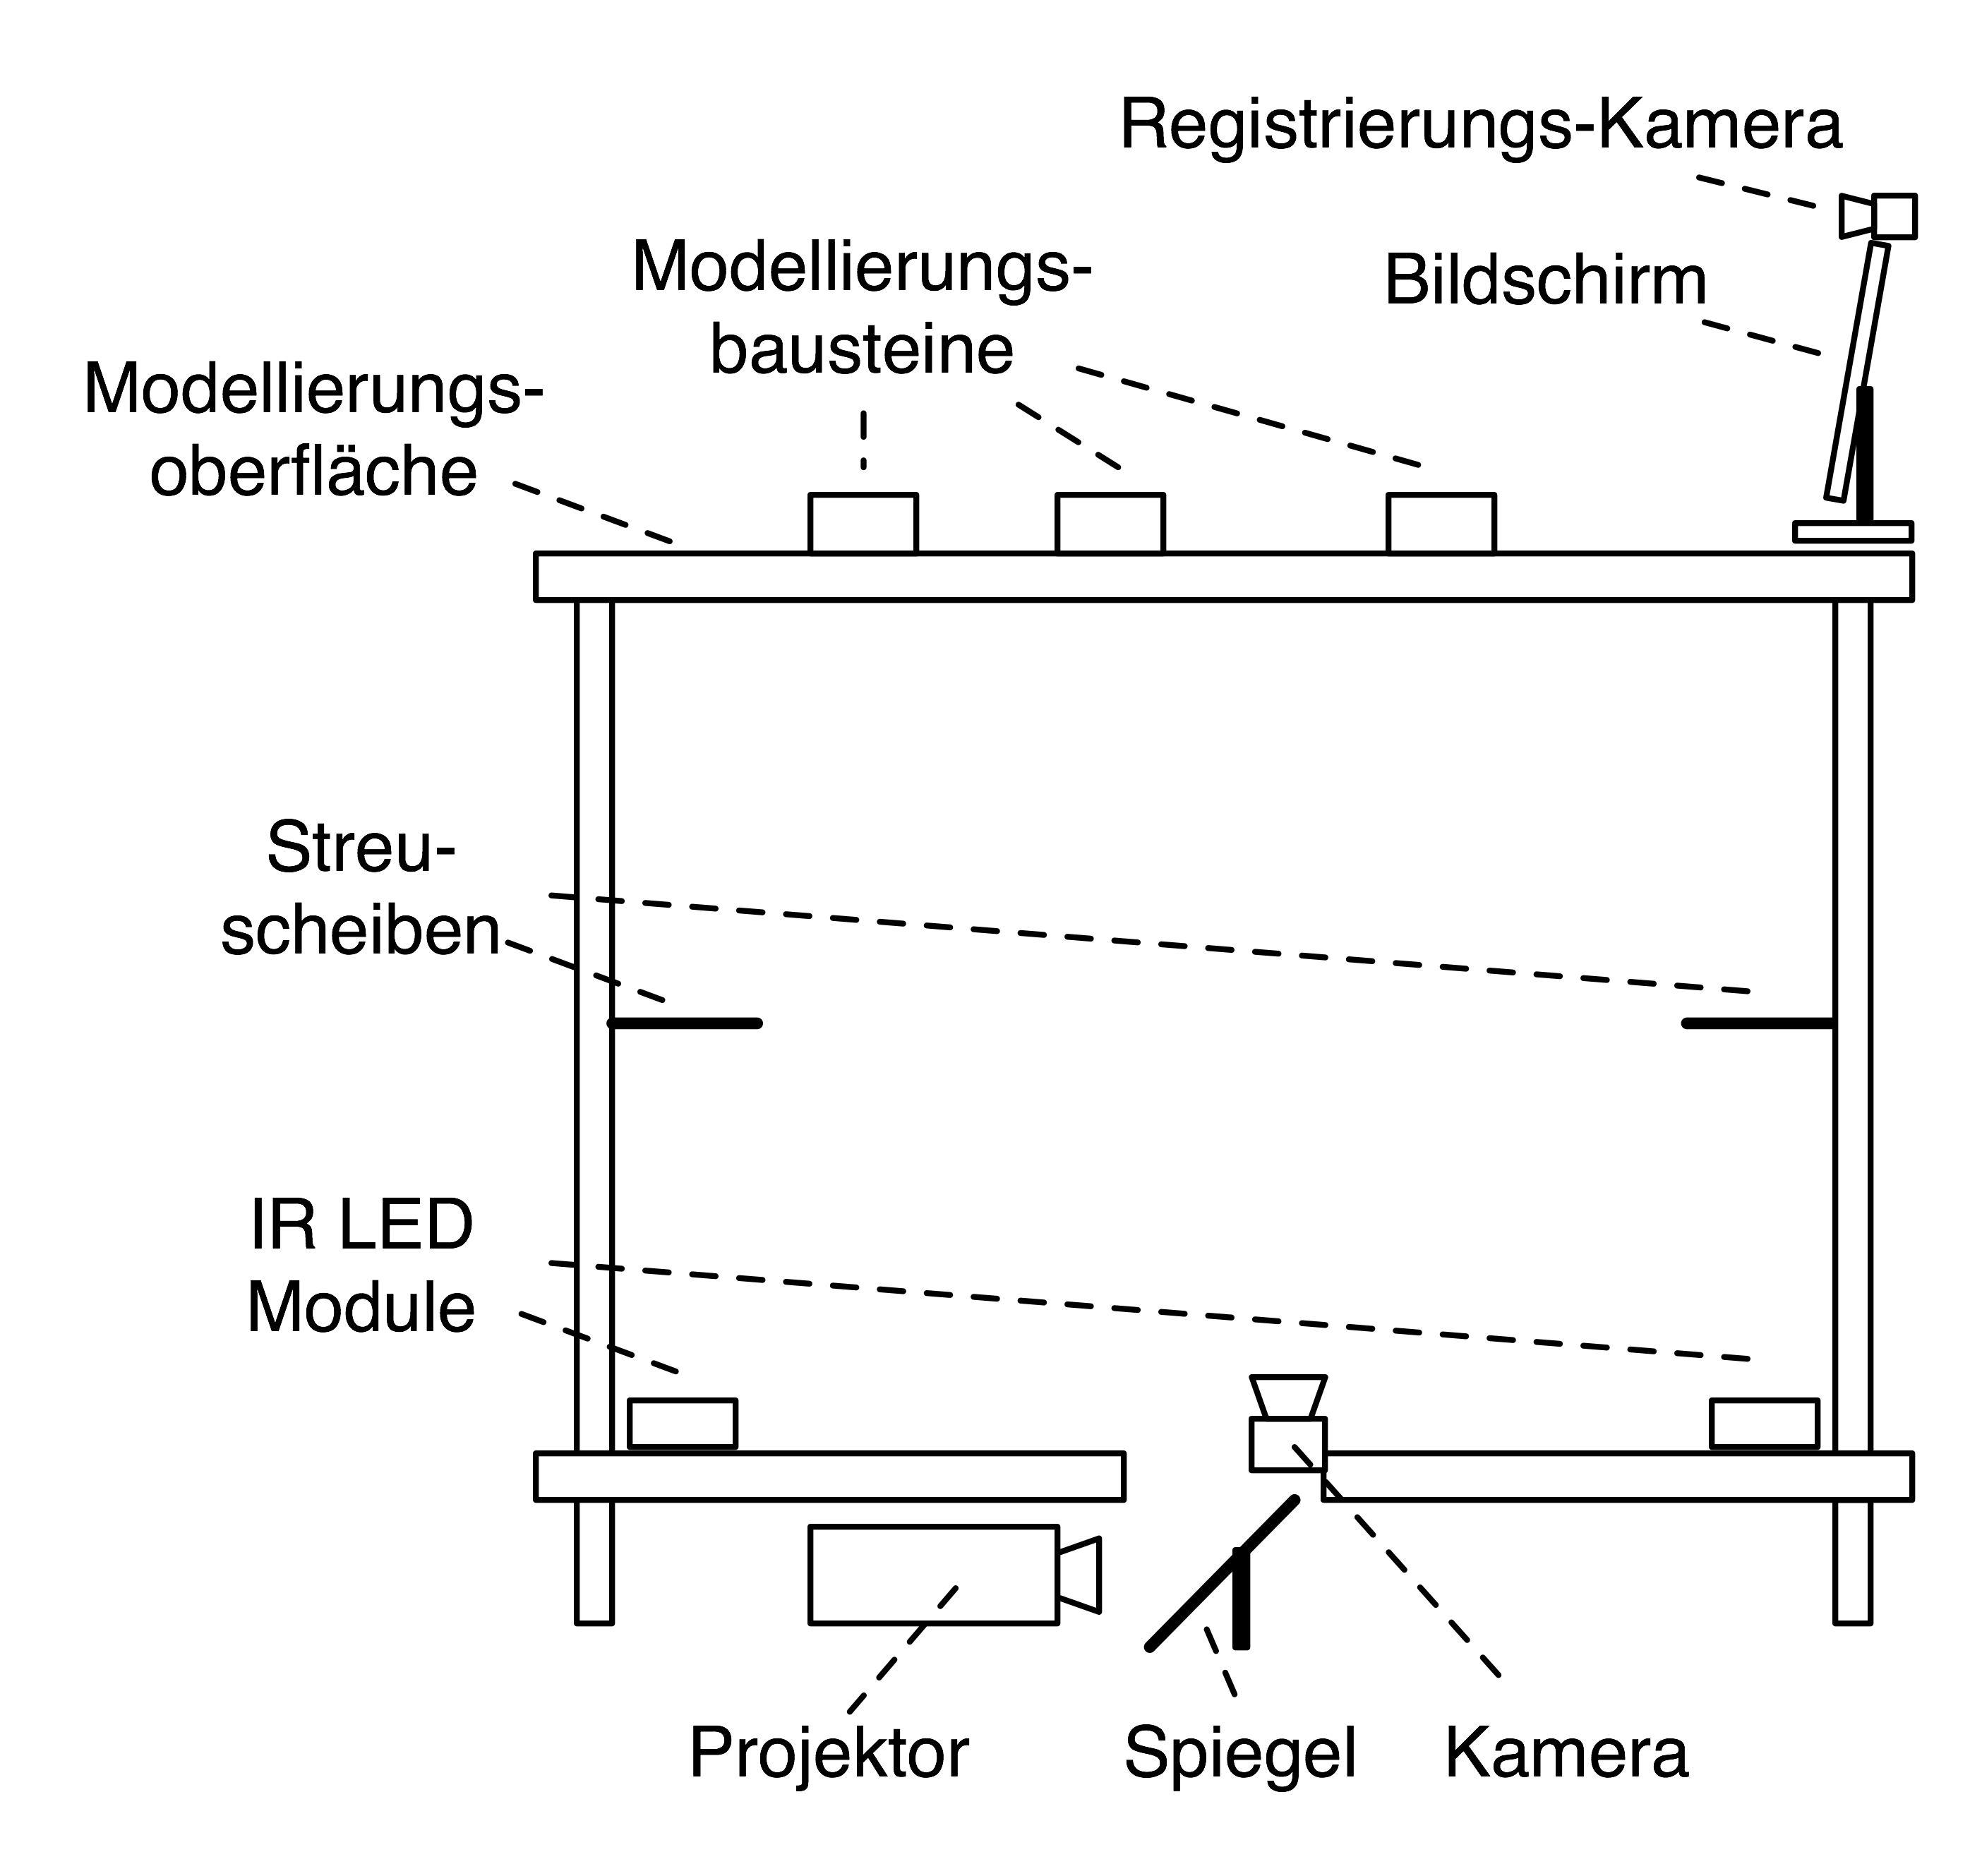
\includegraphics[height=4in]{img/ImplementierungInput/TischSeitenansicht.png}
	\caption{Überblick über den Aufbau des Tabletop Interfaces}
	\label{fig:img_ImplementierungInput_TischSeitenansicht}
\end{figure}

Am Tisch befindet sich zusätzlich ein Bildschirm, auf dem entsprechend der Anforderungen zur Unterstützung der Modellierung Zusatzinformation ausgegeben wird. Eine zweite Kamera, die am Bildschirm sitzt und der unterstützenden Erfassung von Information dient (zum Beispiel der Registrierung von geschachtelten Token wie oben bereits beschrieben).

Das gesamte System ist so zerlegbar, dass es im Kofferraum eines Mittelklassewagens transportiert werden kann. Es werden dazu die Verkleidungsplatten und Tischbeine entfernt, die Tischplatte kann dann direkt auf die Bodenplatte gesetzt und verbunden werden. Das Volumen reduziert sich dabei auf 100 cm x 80 cm x 20 cm, wobei die Tischbeine, die Verkleidungsplatten und der Videoprojektor separat transportiert werden müssen. Ein Zusammenbau des Systems inklusive Kalibrierung der Eingabe- und Ausgabe-Kanäle ist in etwa 30 Minuten möglich.

% subsection Überblick (end)

\subsection{Tokens \& Input-Werkzeuge} % (fold)
\label{sub:tokens_&_input_werkzeuge}

In diesem Abschnitt werden die einzelnen durch die Benutzer manipulierbaren Token-Arten beschrieben. Neben den eigentlichen Modellierungstokens sind dies die Tokens zur Einbettung in Container sowie die Werkzeugtokens, von denen es Ausführungen zur Manipulation des Modells und Tokens zur Auslösung bzw. Kontrolle spezifischer Funktionalitäten gibt.

\subsubsection{Modellierungs-Tokens} %fold 
\label{subs:modellierungs_tokens}

Die eingesetzten Modellierungs-Tokens sind aus nicht transparentem Acrylglas gefertigt. Ihre Außenmaße betragen in etwa (je nach Form) 10 cm x 6 cm in der Grundfläche und 4 cm in der Höhe. Damit ist einerseits eine ausreichende Größe zur Anbringung der ReacTIVision-Codes gewährleistet, andererseits sind noch klein genug, um in einer Hand gehalten und manipuliert werden zu können. Die Codes werden auf der Unterseite der Tokens angebracht und auch von unten erfasst (siehe nächster Abschnitt), um eine Verdeckung der Codes während der Manipulation zu verhindern (siehe Abbildung \ref{fig:img_ImplementierungInput_TokensCodes}).

\begin{figure}[htbp]
	\centering
		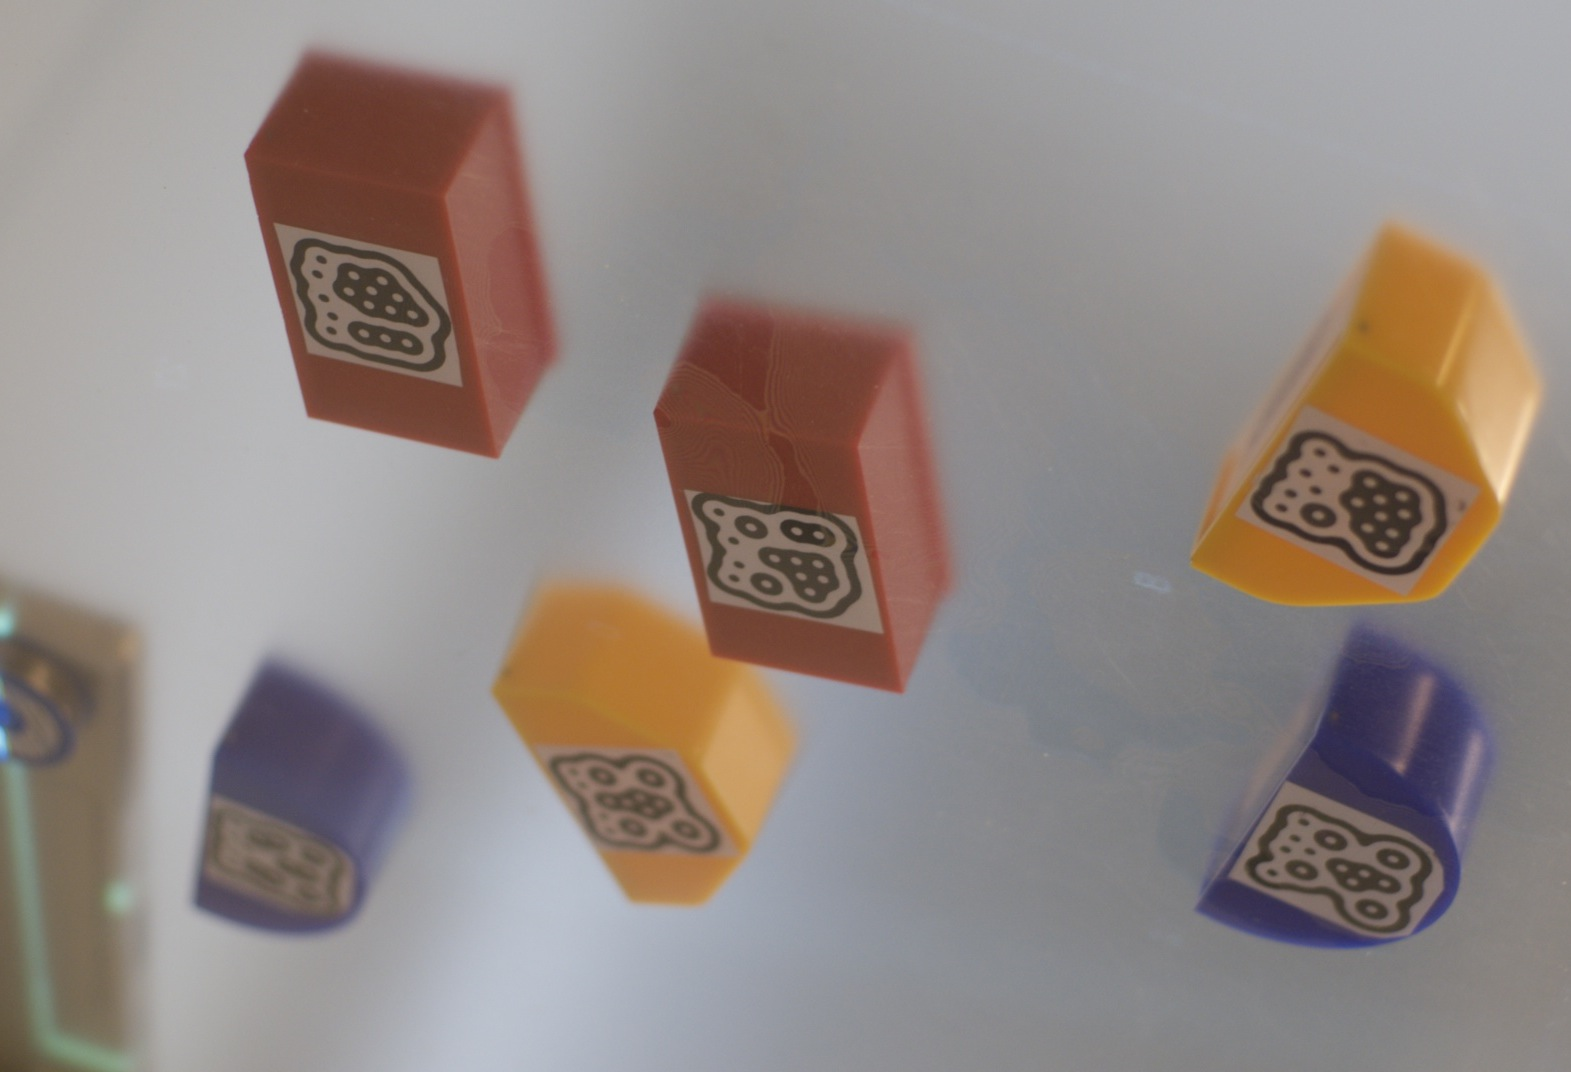
\includegraphics[height=2in]{img/ImplementierungInput/TokensCodes.jpg}
	\caption{An Tokens angebrachte ReacTIVision-Codes zur Identifikation}
	\label{fig:img_ImplementierungInput_TokensCodes}
\end{figure}

\begin{figure}[htbp]
	\centering
		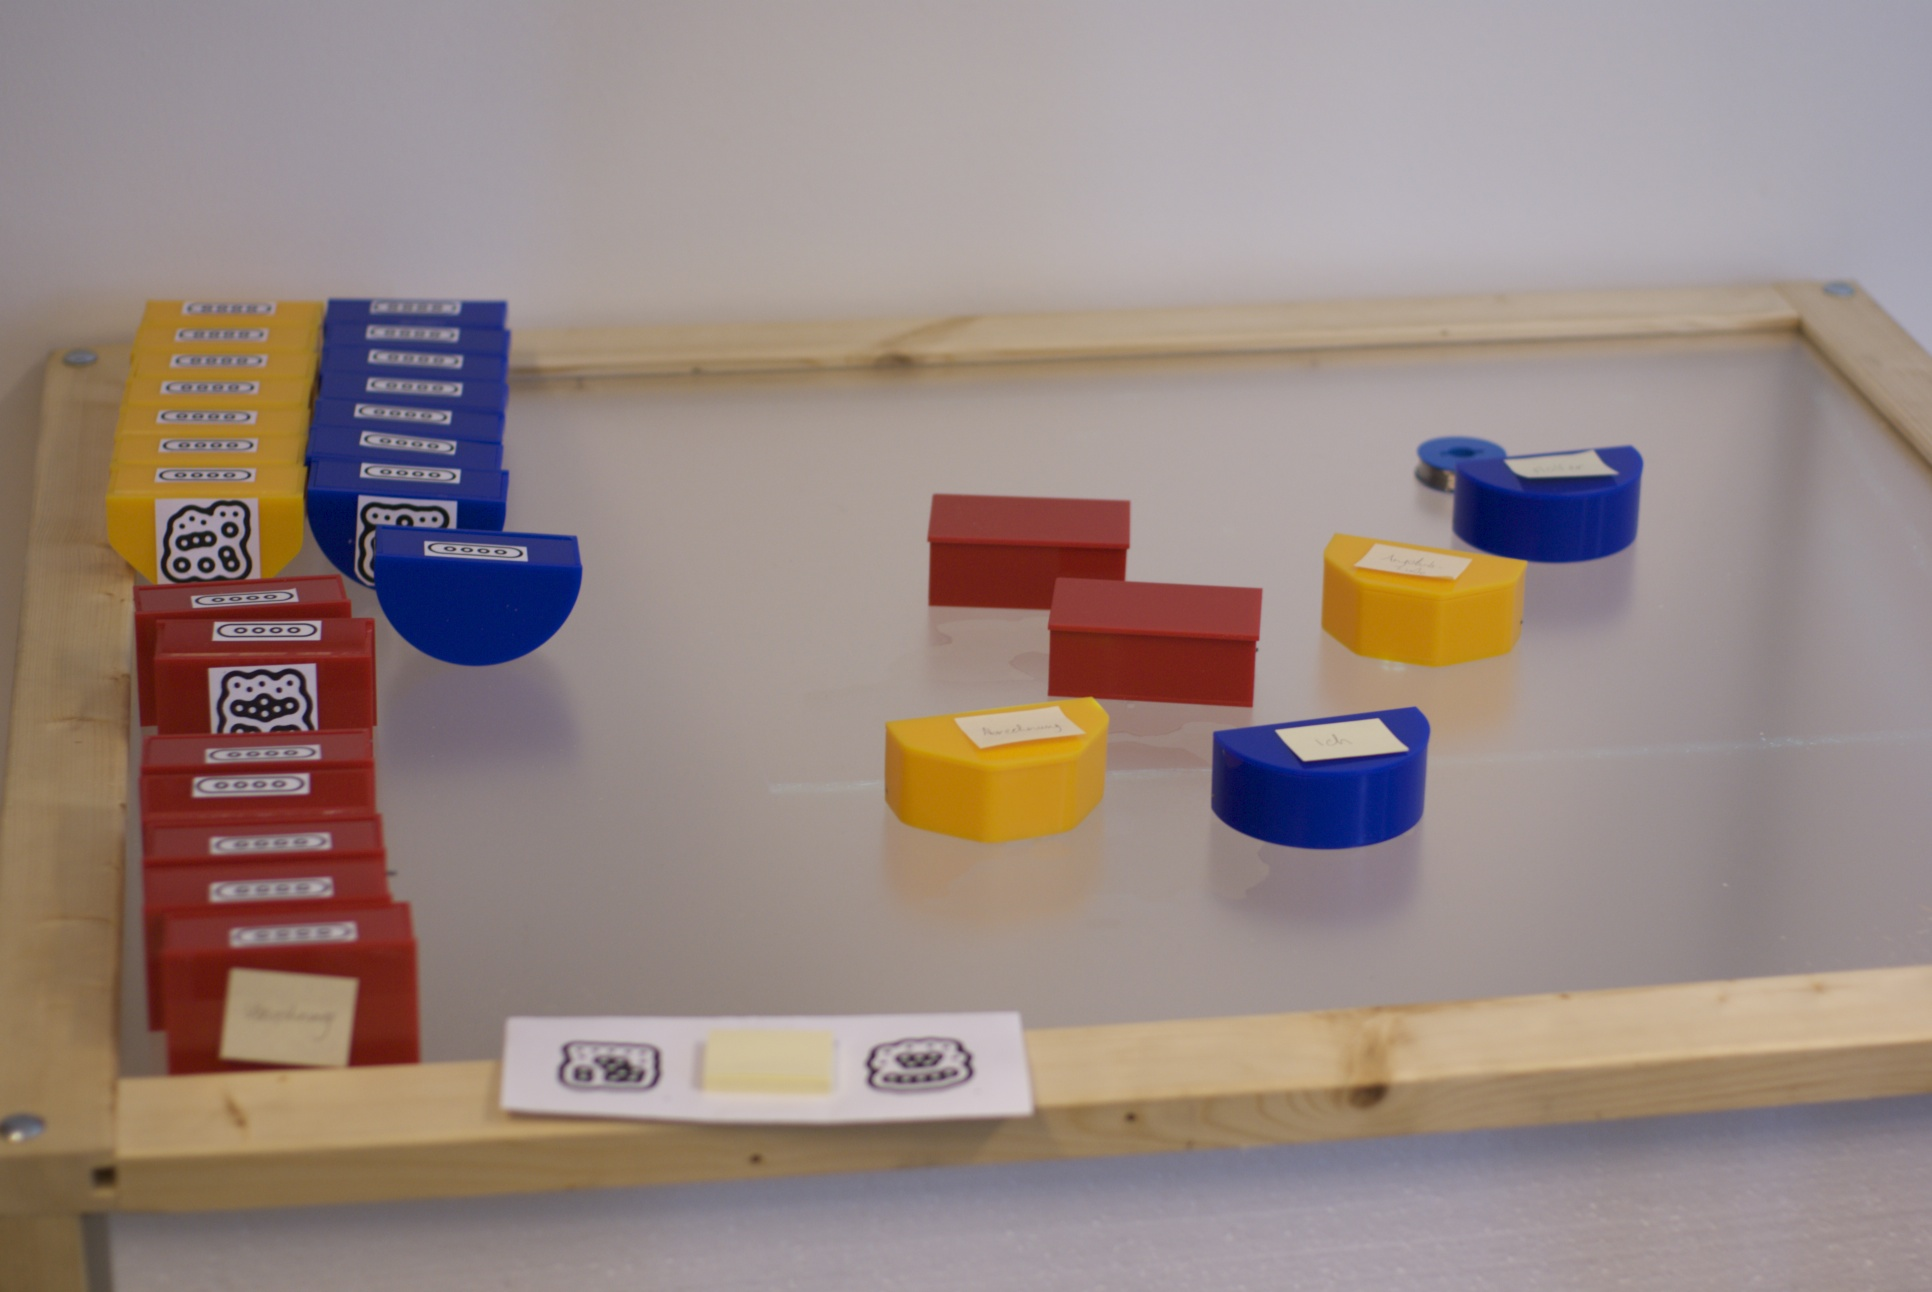
\includegraphics[height=2in]{img/ImplementierungInput/TokenTypes.jpg}
	\caption{Arten von Modellierungstokens}
	\label{fig:img_ImplementierungInput_TokenTypes}
\end{figure}


Die Modellierungs-Tokens wurden in drei Ausführungen gefertigt (siehe Abbildung \ref{fig:img_ImplementierungInput_TokenTypes}). Diese unterscheiden sich in Form und Farbe und können während der Modellierung von den Benutzern frei mit Bedeutung belegt werden. Die Auswahl der Formen und Farben erfolgte inspiriert von den Symbolen gängiger Modellierungsnotationen in Abstimmung mit fertigungstechnischen Einschränkungen. Eine wie in XY (REF von TEI) vorgeschlagene Analyse geeigneter Token-Formen und eine auf diesen Ergebnissen basierende Umsetzung wurde nicht vorgenommen. Die liegt vor allem in der Tatsache begründet, dass sich der Fokus der hier vorgestellten Arbeit im Entwicklungsprozess von einem Werkzeug zur Geschäftsprozessmodellierung (mit vorgegebener Notation) hin zu einem allgemeiner einsetzbaren Werkzeug zur generischen Modellierung konzeptueller Modelle (ohne vorgegebene Notation) entwickelte. Die Auswahl der Token-Formen fiel in die erste Phase, wodurch die Tokens im äußeren Erscheinungsbild an gängige Notationen zur Ablauf-Modellierung angelehnt sind. Die Auswirkung der Token-Form auf die Modellierung scheint aber bei Benutzern ohne Modellierungs-Vorbildung geringen bis keinen Einfluss auf den Modellierungsprozess zu haben (siehe Kapitel XY - Evaluierung).

\begin{figure}[htbp]
	\centering
		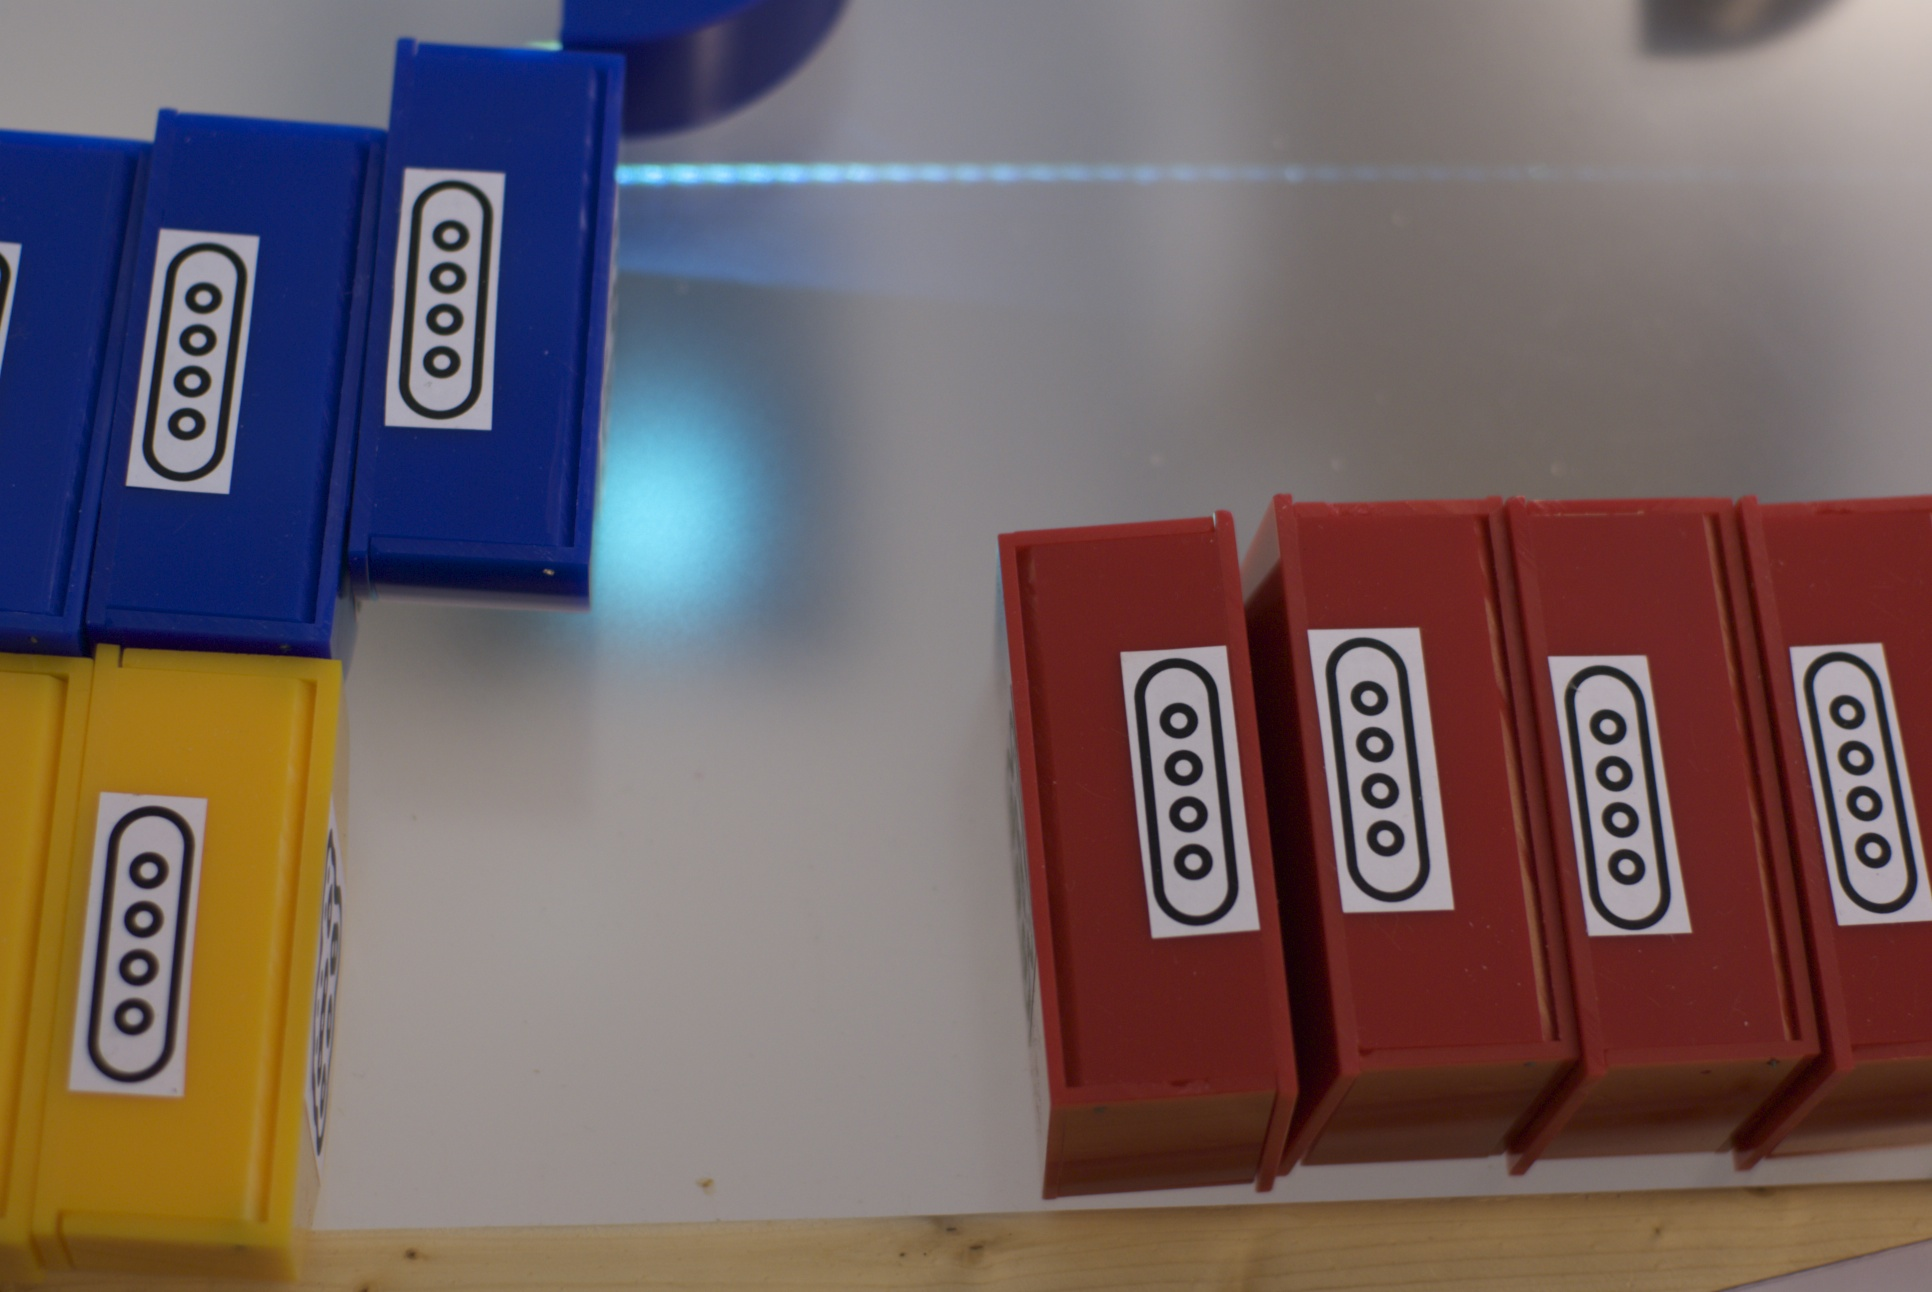
\includegraphics[height=2in]{img/ImplementierungInput/ContainerRueckseite.jpg}
	\caption{Rückwand von Container Tokens}
	\label{fig:img_ImplementierungInput_ContainerRueckseite}
\end{figure}

Wie in der Beschreibung der Anforderungen gefordert und oben bereits beschrieben sind die Modellierungs-Tokens als Container ausgeführt. Im Abschnitt über die Erkennung des Token-Zustands (REF) wurde beschrieben, das beim Einsatz von optischem Tracking eine Möglichkeit geschaffen werden muss, im Kamerabild zu erkennen, ob ein Token geöffnet ist oder nicht. Um den konsequenten Einsatz eines Erkennungsframeworks (ReacTIVision) zu gewährleisten, wird zu diesem Zweck ein zweiter Code eingesetzt (siehe Abbildung \ref{fig:img_ImplementierungInput_ContainerRueckseite}), der nur dann für die Kamera sichtbar wird, wenn das Token geöffnet ist. Hardwareseitig ist dies so umgesetzt, das die Modellierungstokens einen Öffnungsmechanismus besitzen, dessen Schanier nicht am Deckel sitzt (und damit nur diesen beweglich machen würde), sondern an der Bodenplatte, wodurch sich beim Öffnen eines Containers nicht nur der Deckel sondern auch die Hinterwand des Tokens bewegt (siehe Abbildung \ref{fig:img_ImplementierungInput_ContainerToken}). Die Hinterwand kommt im geöffneten Zustand auf der Oberfläche des Tisches zu liegen, wodurch der auf ihr angebrachte zweite Code für die Kamera sichtbar wird. So kann durch das ansich zur Positionsbestimmung eingesetzte optische Trackingsystem zuverlässig auch den Öffnungs-Zustand der Tokens auf der Oberfläche erkennen.

\begin{figure}[htbp]
	\centering
		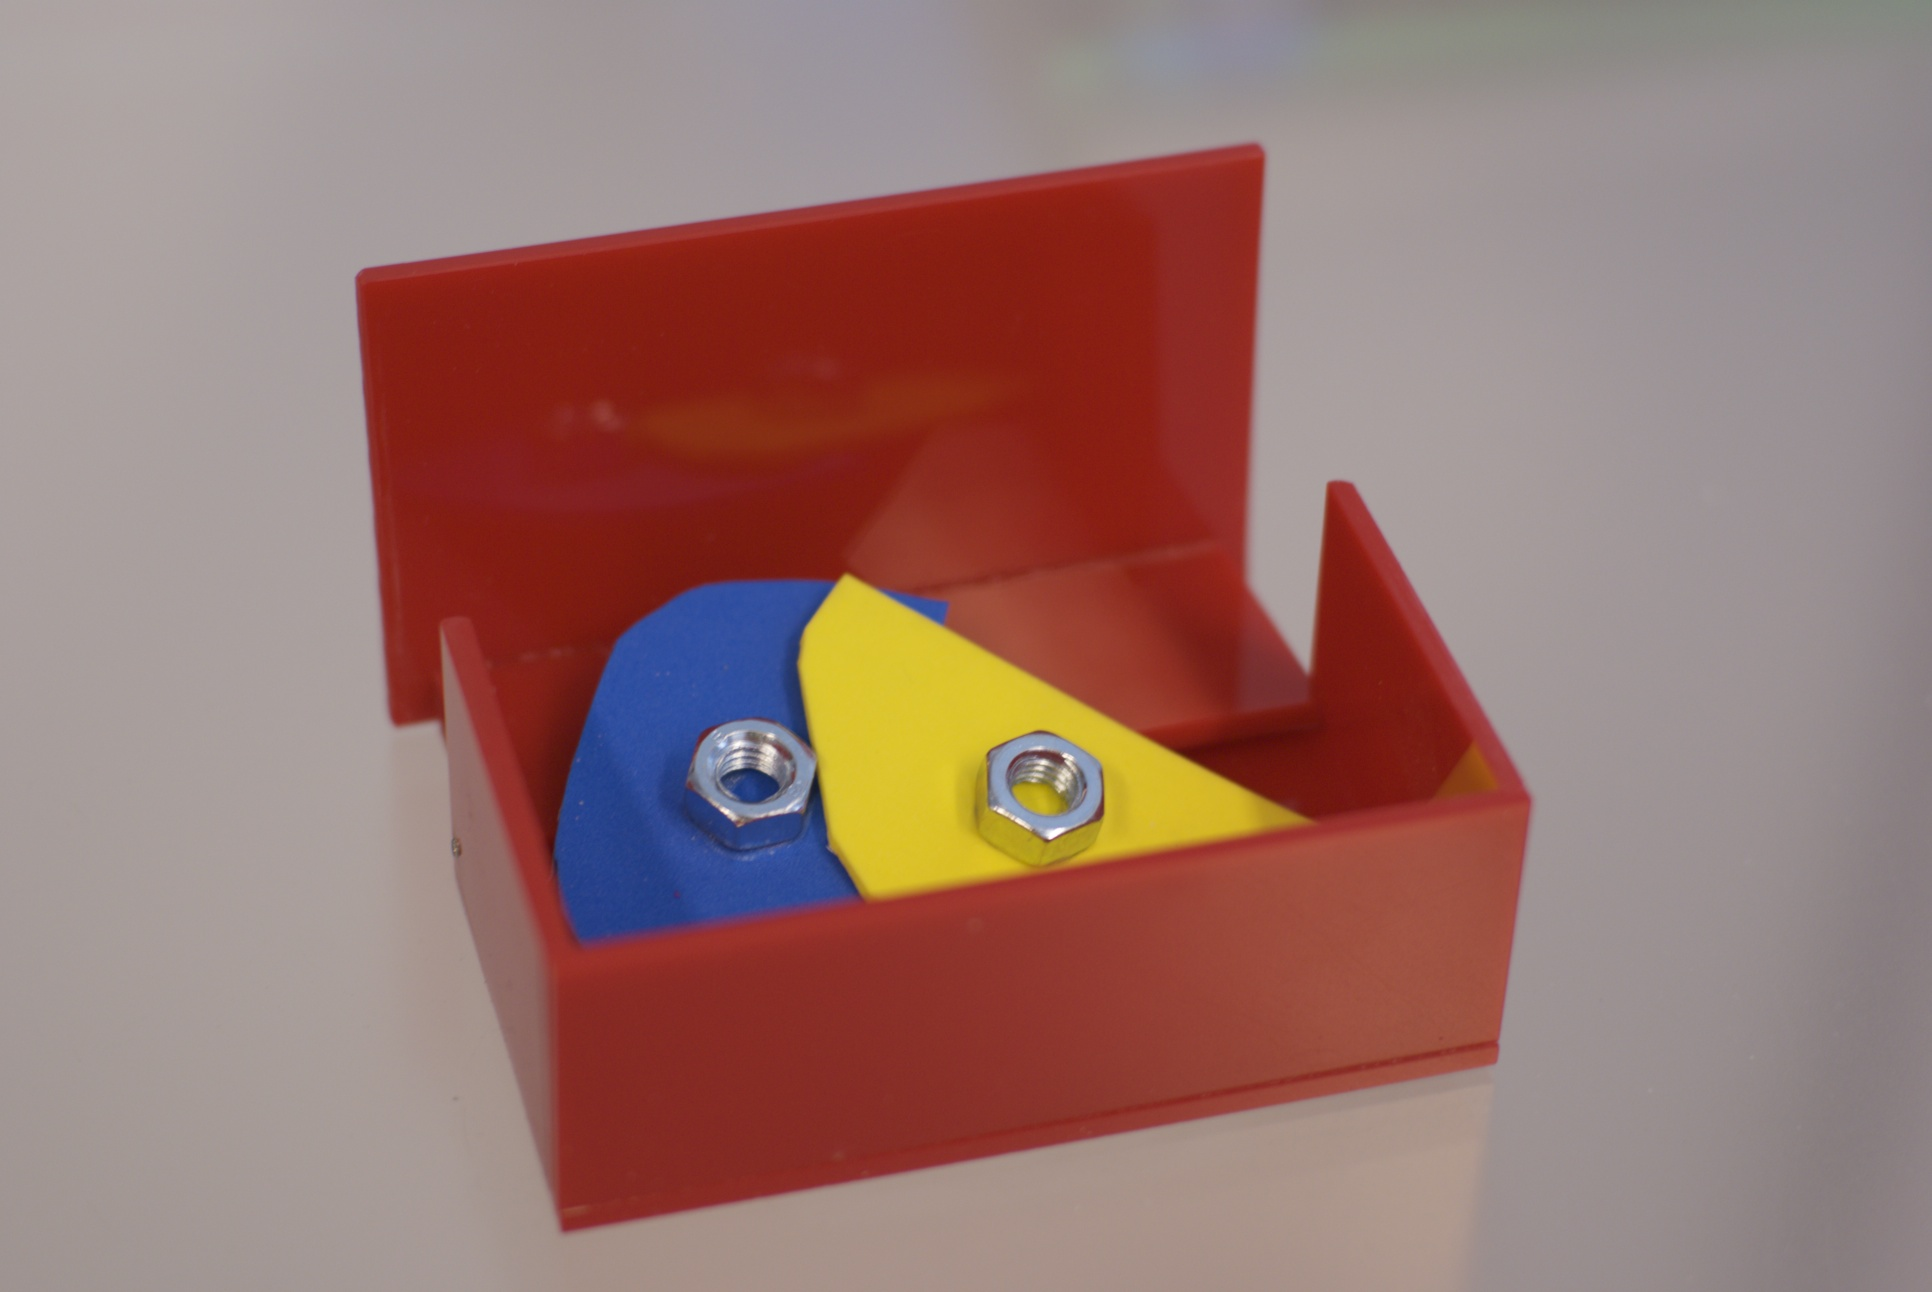
\includegraphics[height=2in]{img/ImplementierungInput/ContainerToken.jpg}
	\caption{Geöffnetes Container Token}
	\label{fig:img_ImplementierungInput_ContainerToken}
\end{figure}

% subsubsection modellierungs_tokens (end)

\subsubsection{Einbettbare Tokens} % (fold)
\label{einbettbare_tokens}

Die einbettbaren Token erlauben wie in Kapitel XY beschrieben die Verschachtelung von Modellen und das Hinzufügen von Zusatzinformation. Sie werden in einem definierten Interaktionsvorgang an Information gebunden und dann in einen Container gelegt. Hinsichtlich des Hardware-Designs sind folgende Anforderungen zu beachten:
\begin{itemize}
	\item Die Token müssen klein genug sein, um auch mehrere Einheiten ein einem Container unterzubringen.
	\item Sie müssen gleichzeitig groß genug sein, um einen ReacTIVision-Code zur eindeutigen Information anzubringen.
	\item Sie müssen so ausgeführt sein, dass haptisch oder akustisch erkennbar ist, ob in einem geschlossenen Container Tokens eingebettet sind oder nicht (z.B. durch Gewicht oder Geräusche beim Schütteln eines Containers).
\end{itemize}

Die einbettbaren Tokens wurden aus flexiblen Kunststoffmatten gefertigt und mit einem Metallstück versehen (siehe Abbildung \ref{fig:img_ImplementierungInput_ContainerToken}), das einerseits als Griff dient und andererseits sowohl das Gewicht erhöht und akustisches Feedback beim Schütteln eines Container-Tokens verursacht. Die einbettbaren Tokens wurden exemplarisch in drei Ausführungen gefertigt, je nach Art und Anzahl der einzubettenden Information kann eine Definition weiterer Tokens sinnvoll sein. Folgende Tokens wurden für den aktuellen Entwicklungsstand des Werkzeugs angefertigt:
\begin{itemize}
	\item Einbettung von Teilmodellen (inhärente Kernfunktionalität des Werkzeugs)
	\item Einbettung von digitalen Ressourcen bzw. Dateien am lokalen Rechner (Erweiterung zur Verknüpfung des Modells mit den realen digitalen Ressourcen aus dem Arbeitskontext)
	\item Einbettung von Fotos (Erweiterung zur Verknüpfung des Modells mit dem realen Arbeitskontext, z.B. mittels Fotos von Arbeitsmitteln oder Personen)
\end{itemize}

Alle Tokens sind auf der Unterseite mit einem ReacTIVision-Code versehen, der sie eindeutig identifiziert. Aufgrund der beschränkten Größe der Tokens ist dieser Code von der Kamera, die die Tischoberfläche erfasst, nur in der Mitte der Oberfläche erfassbar (da dort die geringsten Linsen-Verzerrungen auftreten und der Code somit gerade noch erkannt werden kann). Um etwaige Bedienungsprobleme zu vermeiden, wurde die deshalb die Interaktion mit einbettbaren Tokens (Registrierung, Binden von Information) auf die in Abbildung \ref{fig:img_ImplementierungInput_TischSeitenansicht} dargestellte zweite Kamera ("Registrierungs-Kamera") verlegt, die durch die physische Nähe zu den Modellierenden die Codes der einbettbaren Tokens problemlos erfassen kann.

% subsubsection einbettbare_tokens (end)

\subsubsection{Werkzeug Tokens} % (fold)
\label{ssub:werkzeug_tokens}

Neben den Tokens, die Modellierungsinhalt repräsentieren, wurden auch Tokens angefertigt, der Interaktion mit dem System ansich und der Steuerung der Modellierungsablaufs dienen. Hier sind zwei Arten zu unterscheiden: einerseits gibt es Werkzeuge, die der Manipulation des Modells dienen (z.B. Herstellung von Verbindungen zwischen Tokens, Benennung von Tokens) und andererseits solche, die der Steuerung von modellierungsunterstützender Zusatzfunktionalität dienen (etwa Tokens, die die Rückverfolgung der Modellierungshistorie kontrollieren). Außerdem sind orthogonal zu dieser Klassifizierung noch Tokens zu unterscheiden, die beim Einsatz ein Ereignis auslösen und solche, die die für einen Zustandswechsel des Systems sorgen, solange sie im Einsatz sind (gleich einem Schalter). Im Folgenden werden die einzelnen Werkzeuge beschrieben und den eben definierten Kategorien zugeordnet.

\paragraph{Manipulation des Modellierungsablaufs} % (fold)
\label{par:manipulation_des_modellierungsablaufs}

Die bei der Verwendung des Systems wichtigsten Werkzeug Tokens sind jene, die zur Benennung und Verbindung von Modellierungs-Tokens verwendet werden. 

-- Bild der Auswahl-Werkzeuge --

% paragraph manipulation_des_modellierungsablaufs (end)

\paragraph{Steuerung von Unterstützungsfunktionen} % (fold)
\label{par:steuerung_von_unterstützungsfunktionen}

% paragraph steuerung_von_unterstützungsfunktionen (end)
% subsubsection werkzeug_tokens (end)
% subsection tokens_&_input_werkzeuge (end)

\subsection{Input auf der Tischoberfläche} % (fold)
\label{sub:input_auf_der_tischoberfläche}

Semitransparente Oberfläche, Projektion von unten (Umlenkspiegel), Kamera von unten - Überleitung zur 
Illumination via Interferenz zwischen Beamer und Kamera

\subsubsection{Illumination und Umgebungslichtabhängigkeit} % (fold)
\label{sub:illumination_und_umgebungslichtabhängigkeit}

% subsubsection illumination_und_umgebungslichtabhängigkeit (end)
% subsection input_auf_der_tischoberfläche (end)
% section konzeption_und_umsetzung_der_hardwarekomponenten (end)

\section{Benutzerinteraktion mit dem Werkzeug} % (fold)
\label{sec:benutzerinteraktion_mit_dem_werkzeug}

\subsection{Hinzufügen und Verändern von Modellelementen} % (fold)
\label{sub:hinzufügen_und_verändern_von_modellelementen}

% subsection hinzufügen_und_verändern_von_modellelementen (end)

\subsection{Benennen von Modellelementen} % (fold)
\label{sub:benennen_von_modellelementen}

% subsection benennen_von_modellelementen (end)

\subsection{Verbinden von Modellelementen} % (fold)
\label{sub:verbinden_von_modellelementen}

% subsection verbinden_von_modellelementen (end)

\subsection{Löschen von Elementen und Verbindungen} % (fold)
\label{sub:subsection_name}

% subsection subsection_name (end)

\subsection{Einbettung von Zusatzinformation} % (fold)
\label{sub:einbettung_von_zusatzinformation}

% subsection einbettung_von_zusatzinformation (end)

\subsection{Kontrolle der Modellierungshistorie} % (fold)
\label{sub:kontrolle_der_modellierungshistorie}

% subsection kontrolle_der_modellierungshistorie (end)
% section benutzerinteraktion_mit_dem_werkzeug (end)

\section{Erfassung der Benutzerinteraktion durch Software} % (fold)
\label{sec:erfassung_der_benutzerinteraktion_durch_softfware}

% section erfassung_der_benutzerinteraktion_durch_software (end)

\section{Interpretation der Rohdaten und Stabilisierung der Erkennungsleistung} % (fold)
\label{sec:interpretation_der_rohdaten_und_stabilisierung_der_erkennungsleistung}

% section interpretation_der_rohdaten_und_stabilisierung_der_erkennungsleistung (end)
% chapter input_&_interpretation (end)

\chapter{Ausgabe} % (fold)
\label{cha:visualisierung}

In diesem Kapitel wird die konzeptuelle Ausrichtung und technische Umsetzung jenes Teils des Werkzeugs behandelt, der sich mit der Ausgabe von Information an die Benutzer beschäftigt. Im Bereich der Tangible Interface erfolgt die Ausgabe von Information zumeist kohärent mit dem Eingabemedium, eine physische Trennung zwischen Eingabe- und Ausgabekanälen wie in der herkömmlichen Mensch-Maschine-Interaktion liegt nicht vor \citep{Ullmer00}. \citet{Fishkin04} relativiert die strikte Forderung in seiner Taxonomie für Tangible Interfaces (wie in Abschnitt \ref{sub:tangibles_taxonomien} beschrieben und klassifiziert Benutzungsschnittstellen unter anderem nach dem Grad deren Ein- und Ausgabe-Kohärenz. Dementsprechend sind nicht nur jene Ausgabekanäle Gegenstand dieses Kapitels, die Information in direkter Verbindung mit den Eingabemedien zurückspiegeln, sondern auch jene, die Information auf anderen, nicht-kohärenten Wegen ausgeben.

Im ersten Abschnitt dieses Kapitels werden auf Basis der in Kapitel XY genannten Anforderung an das Werkzeug die den Benutzern mitzuteilenden Informationen identifiziert, noch ohne konkret auf die technologische Realisierung der Ausgabekanäle einzugehen. Im darauf folgenden Abschnitt die technologischen Möglichkeiten zur Ausgabe von Information betrachtet und im Anschluss hinsichtlich ihrer Eignung für die im konkreten Anwendungsfall auszugebende Information bewertet und entsprechend zugeordnet.

Im Anschluss werden auf Basis dieser grundsätzlichen Technologieentscheidung Software-Frameworks beschrieben, die die Realisierung der gewählten Ausgabekanäle ermöglichen. Die Entscheidung für ein konkretes Framework wird auf Basis der funktionalen und nicht-funktionalen Anforderungen an die Ausgabe und deren Umsetzung getroffen. Der letzte Abschnitt beschreibt die eigentliche Umsetzung der Ausgabekanäle mittels der gewählten Technologie und geht die spezifischen Eigenschaften und Implementierungsentscheidungen der vorgestellten Lösung ein.

\section{Auszugebende Information} % (fold)
\label{sec:auszugebende_information}

Den Benutzern des Systems müssen während der Modellierung unterschiedliche Information zur Verfügung gestellt werden. Einerseits ist dies Information, die das Modell selbst betrifft, andererseits muss auch Information ausgegeben werden, die Aspekte des Modellierungsablaufs beschreibt oder unterstützt.

Die das Modell betreffende Information muss folgende Aspekte abdecken:
\begin{itemize}
 \item Die Modellelemente betreffende Information (Art, Position, Benennung)
 \item Die Verbinder betreffende Information (Art, Endpunkte, Benennung)
 \item Einbettete Elemente betreffene Information (Art, Inhalt, Container)
\end{itemize}

Zur Unterstützung des Modellierungsablaufs müssen folgende Aspekte zur Verfügung gestellt werden:
\begin{itemize}
 \item Information über vergangene Modellzustände
 \item Information zur die Wiederherstellung von Modellzuständen
\end{itemize}

Hier wird bewusst noch nicht auf die technische Umsetzung dieser Ausgabe eingegangen. In den folgenen Abschnitten wird erörtert, welche grundlegenden Technologien in Frage kommen, bevor auf Basis deren Eignung und den Vorgaben aus den Technologieentscheidungen zur Informationseingabe eine konkrete Lösung ausgewählt wird.

% section auszugebende_information (end)

\section{Technologische Grundlage der Ausgabe} % (fold)
\label{sec:technologische_grundlage_der_visualisierung}

Bei der Ausgabe von Information muss im Falle von Tangible Interfaces zwischen Ansätzen mit unterschiedlich stark ausgeprägter Kohärenz mit den Eingabekanälen unterschieden werden. Unter Kohärenz ist hier zu verstehen, das jene Artefakte, die zur Eingabe verwendet werden gleichzeitig auch die Reaktion des Systems -- also die Ausgabe -- wiederspiegeln. In der von \citet{Fishkin04} vorgeschlagenen Taxonomie (siehe Abschnitt XY) werden in der Dimension "Embodiment" auch Werkzeuge als Tangible Interfaces klassifiziert, bei denen die Ausgabe vollständig von der Eingabe entkoppelt ist. Diesem Verständnis folgt auch diese Arbeit.

Bei Tabletop Interfaces bietet sich die Tischoberfläche als Ausgabemedium an, um kohärente Informationsausgabe zu gewährleisten. Die Tischoberfläche dient hier wie in Kapitel \ref{cha:input_&_interpretation} beschrieben der Eingabe und kann durch unterschiedliche technologische Maßnahme auch zur Ausgabe genutzt werden. Eine weitere Möglichkeit, die Ausgabekohärenz bei Tabletop Interfaces sicherzustellen bzw. zu steigern, ist die Verwendung der zur Interaktion mit dem System verwendeten Tokens als Ausgabemedium. Je nach verfolgtem Ansatz (bzw. einer Kombination) sind unterschiedliche technische Maßnahmen zu setzen. In den folgenden Abschnitten werden die hier erwähnten grundsätzlich in Frage kommenden Ansätze betrachtet und im Anschluss hinsichtlich ihrer Eignung für das hier entwickelte System beurteilt. Basierend auf der grundsätzlichen Technologieentscheidung werden im Anschluss unterschiedliche technische Lösungen zur Erfüllung der Anforderungen beschrieben.

\subsection{Ansätze zur kohärenten Ausgabe} % (fold)
\label{sub:kohärente_ausgabe}

In diesem Abschnitt werden Ausgabeansätze behandelt, die nach \citep{Fishkin04} in der Embodiment-Dimension den Ausprägungen "full" oder "nearby" zuzuordnen sind. Die Ausgabe erfolgt bei den hier vorgestellten Ansätzen also direkt über die Eingabetokens ("full") oder ist räumlich unmittelbar in der Umgebung der Tokens angesiedelt.

\subsubsection{Darstellung auf der Tischoberfläche} % (fold)
\label{ssub:darstellung_auf_der_tischoberfläche}

Bei Tabletop-Interfaces ist die Nutzung der Tischoberfläche ein naheliegender und gängiger Ansatz zur Realisierung der Ausgabekanäle. Die Ausgabe erfolgt hierbei visuell, also durch die Darstellung der auszugebenden Information. Ein derartig ausgestaltetes Interface ist hinsichtlich seiner Ausprägung in der Embodiment-Dimension als "nearby" zu klassifizieren. Technologisch kommen zur Darstellung horizontal eingesetzte Bildschirme oder Oberflächen, auf die projiziert werden kann, in Frage.

Bei der Verwendung von Bildschirmen sind die Größe der zur Anzeige verwendbaren Oberfläche sowie die zur Anzeige verfügbare Auflösung (also indirekt die Größe eines Bildpunktes) wesentliche Kriterien. Bei heute verfügbaren LCD-Modulen mit Größen bis zu 132 cm in der Diagonale und Auflösungen von 1920 x 1080 Bildpunkten ist die Technologie soweit ausgereift und verfügbar, das dieser Ansatz grundsätzlich für den Einsatz in Tabletop Interfaces in Frage kommt. Vorteile sind die geringe Bauhöhe der Ausgabeeinheit (im Vergleich zu den im Folgenden vorgestellten Projektions-Lösungen). Nachteile sind die relative geringe Leuchtstärke, die einen Einsatz bei Tageslichtbedingungen schwierig machen sowie die Blickwinkelabhängigkeit, die bei horizontalem Einbau der Anzeigeeinheit stärker zum Tragen kommt als bei herkömmlicher vertikaler Verwendung.

Als Alternative zur Verwendung von aktiven Anzeigeeinheiten können Projektoren verwendet werden, die die darzustellende Information auf die Tischoberfläche projizieren. Hier ist zwischen Lösungen zu unterscheiden, bei denen die Projektion von oben erfolgt und jenen, die von unten auf eine durchscheinende Tischoberfläche projizieren. Bei ersteren muss der Projektor in ausreichender Höhe über der Tischoberfläche angebracht werden, um das projizierte Bild die notwendige Fläche abdecken zu lassen. Bei beschränkter Höhe nach oben kann ein Projektor mit Weitwinkelobjektiv oder ein Umlenkspiegel benutzt werden, der durch eine Vergrößerung des Abstands zwischen Projektor und Oberfläche auf einer nicht vertikalen Achse die notwendige Bauhöhe reduziert. Der größte Nachteil dieser Lösung ist die Abschattung der projizierten Information bei Manpulationen der Tokens auf der Oberfläche. Um dies zu vermeiden kann auch von unten auf eine durchscheinende Oberfläche projiziert werden. Bei diesem Lösungsansatz kommt es zu keinerlei Abschattungen, die Information wird wie bei Einsatz eines Bildschirms ständig angezeigt. Nachteilig wirkt sich hier der durch den Einsatz einer durchscheinenden Oberfläche verursachte Leuchtkraftverlust aus. Bei dieser Form der Projektion wird immer ein Teil des durch den Projektor ausgestrahlten Lichts von der Oberfläche nach unten zurück reflektiert. Im Gegensatz zur Projektion von oben ist dadurch der Kontrast der Darstellung wesentlich geringer. Für den Einsatz unter Tageslichtbedingungen erscheint also der erstgenannte Ansatz generell besser geeignet. Kritischer ist bei der Projektion von unten der notwendige Abstand zwischen Projektor und Tisch, da sich dieser direkt auf die Höhe des Tisches auswirkt. Um eine akzeptable Bauhöhe zu erreichen -- also den Tisch durch durchschnittliche große Personen bedienbar zu halten (Höhe nicht mehr als etwa 100 cm) -- ist hier der Einsatz eines Umlenkspiegels nahezu unabdingbar. Beiden Projektions-Ansätzen gleich ist, dass die abzudeckende Oberfläche variabel durch den Abstand des Projektors gewählt werden kann. Grenzen sind hier nach unten die Fokussierbarkeit des Projektors bei kleinen Abständen und nach oben die Abnahme der Projektionshelligkeit bei großen Abständen. Bei großen Oberflächen ist zudem auf die verfügbare Auflösung des Projektors zu achten, da die Größe eines Bildpunktes mit zunehmendem Abstand so ansteigt, dass eine feinauflösende Projektion der Information auf der Oberfläche nicht mehr möglich ist.

% subsubsection darstellung_auf_der_tischoberfläche (end)

\subsubsection{Aktive Anzeige auf Tokens} % (fold)
\label{ssub:aktive_anzeige_auf_tokens}

Alternativ zur Darstellung auf der Tischoberfläche können bei Tabletop-Interfaces auch die Tokens selbst als Ausgabekanal dienen. Die hier das Eingabemedium gleich dem Ausgabemedium ist, ist diese Form der Ausgabe hinsichlich der Embodiment-Dimension in die Ausprägung "full" einzuordnen. Technologisch können je nach Art der darzustellenden Information Tokens mit Displays ausgestattet werden oder lediglich visuelle Statusanzeigen beinhalten, die Feedback über den aktuellen Zustand des Tokens geben. In beiden Fällen müssen die Tokens generell mit Elektronik und Energieversorgung ausgestattet sein und die Möglichkeit haben, selbst oder über eine Verbindung mit der Infrastruktur ihren Zustand festzustellen.

Um textuelle oder grafische Information auf Tokens darzustellen ist die Verwendung von Displays notwendig. Bei der Verwendung von herkömmlichen LCD-Displays ist durch die notwendige Hintergrundbeleuchtung sowie der notwendigen Stromversorgung zur Aufrechterhaltung der Anzeige der Energieverbrauch verhältnismäßig hoch. Alternativ können neuere Technologien wie OLED- (REF) oder eInk-Displays (REF) verwendet werden. OLEDs bestehen aus organischen Materialien und benötigen keine Hintergrundbeleuchtung, das das Material selbst Licht emmitiert. eInk verwendet eine papierartige Oberfläche zur Anzeige, strahlt selbst kein Licht aus und ist deshalb auf Umgebungshelligkeit zur Verwendung angewiesen. eInk bietet in hellen Umgebungen die besten Kontrastverhältnisse (vergleichbar mit bedrucktem Papier) kann allerdings beim heutigen Stand der Entwickung keine Farben darstellen. Der größte Vorteil von eInk liegt in der Eigenschaft, dass die Anzeige auch ohne Energieversorgung aufrecht bleibt -- Energie ist lediglich zur Änderung des Display-Inhalts notwendig.

Durch das Wegfallen der Hintergrundbeleuchtung sind OLED- und eInk-Displays wesentlich dünner als LCD-Module und können auch auf nicht ebenen Oberflächen angebracht werden. Allen drei Ansätzen gleich ist, dass zur Ansteuerung des Anzeigemoduls Elektronik notwendig ist, die die darzustellende Information auf die zur Verfügung stehen Bildpunkte abbildet und das Display entsprechend ansteuert.

Neben der Verwendung eines Displays kann der Status eines Tokens auch mit Leuchtanzeigen in der Form von LEDs visualisiert werden. Der Nachteil dieses Ansatzes ist die schwierige Realisierbarkeit von komplexen Statusanzeigen - durch die auf zwei Zustände (ein/aus) beschränkte Aussagekraft einer LED sind andere als bipolare Visualisierungen schwer zu realisieren. Möglich ist die Verwendung von mehreren LEDs, wobei diese rasch schwer erfassbar wird, wenn dadurch mehrere voneinander unabhängige Aussagen visualisiert werden. Lediglich die Kopplung mehrere LEDs zur aussagekräftigen Visualisierung von dynamischen Zuständen hat sich als intuitiv erfassbar und verständlich erwiesen (REF Zuckerman Flow Blocks). So können gekopplete LEDs z.B. dazu verwendet werden, Flussrichtungen von Ressourcenströmen anzuzeigen, indem eine LED-Reihe entwender von links nach rechts oder von rechts nach links angesteuert wird. Auch beim Einsatz von LEDs ist einer ständige Energieversorgung notwendig. Zur Reduktion des Energieverbrauchs können wiederum die oben genannten Alternativ-Technologien OLED und eInk zum Einsatz kommen, wobei diese aktuell nicht in den Bauformen herkömmlicher LEDs angeboten werden. eInk-Anzeigen eignen sich aufgrund ihrer langsamen Schaltdauer außerdem nicht für die Realisierung dynamischer Anzeigen.

% subsubsection aktive_anzeige_auf_tokens (end)

\subsubsection{Token mit Aktuatoren} % (fold)
\label{ssub:tokens_mit_aktuatoren}

Neben der Verwendung von Displays zur Realisierung eines "full embodied" Ausgabekanals können Tokens auch mit Aktuatoren ausgestattet werden, die es erlauben, das Token bzw. dessen Verhalten selbst ohne direkte Benutzerinteraktion zu beeinflussen. Beispiele für Aktuatoren sind unter anderem Vibrationsmodule oder mechanische Einheiten zur Veränderung der äußeren Form des Tokens oder dessen Position (auf der Tischoberfläche). Der Einsatz von Aktuatoren ist ob der technologischen und anwendungsspezifischen Vielfalt nicht generisch beschreibbar wie das bei reinen optischen Anzeigeeinheiten der Fall war. Aktuatoren müssen auf den jeweiligen Anwendungsfall abgestimmt sein. Ihr Einsatz ist im Allgemeinen eher disruptiv, unterbricht durch die vom Benutzer nicht selbst ausgelöste Interaktion dessen aktuelle Aktivität und zieht die Aufmerksamkeit auf sich. Dies kann im einzelnen Anwendungsfall erwünscht sein, kann aber zu unerwünschten Effekten bei der Verwendbarkeit des Systems führen.

Wie bei Anzeigemodulen müssen auch hier die Tokens mit Energieversorgung ausgestattet sein und mit Elektronik integriert werden, die für die Ansteuerung der Aktuatoren sorgt.

Im Bereich der Tabletop Interfaces ist die Verwendung von Aktuatoren eher selten anzutreffen. Im Bereich der Ambient Interfaces kann der Einsatz von Aktuatoren aber sinnvoll sein, wenn sich das Interface so in die Umgebung seines Einsatzbereichs integrieren kann (REF Bsp ... Ferscha Blubbersäule?).

% subsubsection tokens_mit_aktuatoren (end)
% subsection kohärente_ausgabe (end)

\subsection{Ansätze zur entkoppelten Ausgabe} % (fold)
\label{sub:entkoppelte_ausgabe}

Ansätze zur enkoppelten Ausgabe sind solche, die von \citet{Fishkin04} in seiner Taxonomie in der Embodiment-Dimension unter den Ausprägungen "environment" oder "distant" eingeordnet werden. 

"Environmental Embodiment" ist dann gegeben, wenn Eingabe- und Ausgabekanäle räumlich nicht kohärent sind, aber Eingaben trotzdem offensichtlich Reaktionen in der unmittelbnaren Umgebung auslösen. Klassische von Fishkin genannte Ansätze sind hier Audiokanäle aber auch die Veränderung von Umgebungslicht oder Temperatur. Auch olfaktorische Interfaces wären in diese Kategorie einzuordnen. In den folgenden Abschnitten werden jedoch ausschließlich audio-basierte Kanäle beschrieben, da diese im Bereich der Tabletop Interfaces Relevanz besitzen (etwa in REF reacTable und REF TEI Paper von Däne)

Die Ausprägung "distant" kennzeichnet Ansätze, in denen die Eingabekanäle räumlich von den Ausgabekanälen vollkommen enkoppelt sind bzw. entkoppelt werden können. Ein Kriterium zur Einordung eines Ansatzes unter "distant" ist, dass Benutzer zur Beobachtung der Ausgabe nicht mehr die Eingabe im Blickfeld haben können (was bei allen anderen Ausprägungen möglich ist). Klassische Vertreter dieses Ansatzes sind alle Ansätze die auf der Darstellung von Information auf herkömmlichen Bildschirmen oder Projektionsflächen basieren.

\subsubsection{Darstellung auf Monitoren} % (fold)
\label{ssub:tokens_mit_aktuatoren}

Bei der Darstellung von Information auf Bildschirmen kommen die auch in der herkömmlichen Desktop-basierten Mensch-Maschine-Interaktion gängigen Anzeigetechnologien zur Anwendung. Im Kontext von Tabletop Interfaces ist bei Monitoren auf die Sichtbarkeit der Information für alle an der Interaktion beteiligten Personen zu achten -- diese ist nicht nur von der Entfernung zum Monitor abhängig sondern bei den heute gängigen LCD-Displays auch vom Blickwinkel. Gegebenenfalls müssen mehrere Monitore verwendet werden, auf denen entweder simultan die gleiche  Information dargestellt wird oder -- abhängig von der Anwendung -- lediglich für die jeweils eingenommene Perspektive relevante Information angezeigt wird. Mit Monitoren kann auch eine vollständig räumlich entkoppelte Darstellung realisiert werden, indem die darzustellende Information auf entfernte Displays übertragen wird. So kann zum Beispiel die Interaktion auf einem Tabletop Interface bzw. deren Auswirkungen auch räumlich entfernt verfolgt werden.

Generell muss bei entkoppelten Ausgabekanälen darauf geachtet werden, dass bei Interaktionen mit den tangiblen Eingabekanälen entsprechend eindeutig zuzuordnendes Feedback über die Ausgabekanäle rückgespiegelt wird. Bei Tabletop Interfaces ist hierbei (wiederum abgängig von der Anwendung) eine schematische Darstellung der Tischoberfläche mit einer Kenntlichmachung des Bereichs, in dem eine Interaktion erkannt wurde, sinnvoll.

% subsubsection tokens_mit_aktuatoren (end)

\subsubsection{Projektion auf entfernte Oberflächen} % (fold)
\label{ssub:tokens_mit_aktuatoren}

Bei Ausgabe mittels Projektion auf entfernte Oberfläche (im Sinne von Oberflächen, die nicht dem eigentlichen Interface zuzuordnen sind) sind Aspekte wie Größe des Bildes oder Blickwinkelabhängigkeit der Darstellung meist keine Herausforderung. Mit einem Projektor können zumeist alle Benutzer ausreichend mit Information bedient werden. Ansonsten gelten die obigen Ausführungen hinsichtlich eindeutig zuzuordnendem Feedbacks analog.

Bei individueller Nutzung eines Tangible Interfaces ist in der Verwendung von Bildschirm oder Projektor noch ein unterschiedlich hoher Grad an Privatheit der Ausgabekanäle festzustellen. Während Bildschirme eher dem mit dem System interagierenden Individuum als Ausgabekanal vorbehalten bleiben, sind projezierte Informationen quasi öffentlich verfügbar. Abhängig vom Anwendungsszenario des Tangible Interfaces kann dies erwünscht sein oder nicht.

% subsubsection tokens_mit_aktuatoren (end)

\subsubsection{Audio-basierte Ausgabekanäle} % (fold)
\label{ssub:tokens_mit_aktuatoren}

% subsubsection tokens_mit_aktuatoren (end)

% subsection entkoppelte_ausgabe (end)

\subsection{Technologie-Entscheidung} % (fold)
\label{sub:output_ansatz_entscheidung}

% subsection output_ansatz_entscheidung (end)

\subsection{Frameworks zur Ausgabe} % (fold)
\label{sub:frameworks_zur_ausgabe}

\subsubsection{In Frage kommende Frameworks} % (fold)
\label{ssub:in_frage_kommende_frameworks}

--> JHotDraw + evtl. andere Frameworks aus KnowIT-Diplomarbeit

\paragraph{JHotDraw} % (fold)
\label{par:jhotdraw}

% paragraph jhotdraw (end)

\subsubsection{Framework-Entscheidung} % (fold)
\label{ssub:output:framework_entscheidung}

% subsubsection output_framework_entscheidung (end)
% subsubsetion in_frage_kommende_frameworks (end)

% subsection subsection_name (end)
% subsubsection jhotdraw (end)

% subsection frameworks_zur_ausgabe (end)

% section technologische_grundlage_der_visualisierung (end)

\section{Ausgabe von Information} % (fold)
\label{sec:ausgabe_von_information}

\subsection{Konzept} % (fold)
\label{sub:ausgabe_konzept}

Dual View
% subsection ausgabe_konzept (end)

\subsection{Architekur} % (fold)
\label{sub:architekur}

Modularchitektur beeinflusst von den Vorgaben der Entwurfsmuster in JHotDraw
% subsection architekur (end)

\subsection{Ausgabe von Information zum Modell} % (fold)
\label{sub:ausgabe_von_information_zum_modell}

\subsubsection{Information zu Modellelementen} % (fold)
\label{ssub:information_zu_modellelemeenten}

% subsubsection information_zu_modellelementen (end)

\subsubsection{Information zu Verbindern} % (fold)
\label{ssub:information_zu_verbindern}

% subsubsection information_zu_verbindern (end)
% subsection ausgabe_von_information_zum_modell (end)

\subsection{Ausgabe zur Kontrolle des Systems} % (fold)
\label{sub:ausgabe_zur_kontrolle_des_systems}

\subsubsection{Zustandsmeldungen} % (fold)
\label{ssub:zustandsmeldungen}
Löschmodus etc.

% subsubsection zustandsmeldungen (end)

\subsubsection{Wiederherstellungsunterstützung} % (fold)
\label{ssub:wiederherstellungsunterstützung}

% subsubsection wiederherstellungsunterstützung (end)
% subsection ausgabe_zur_kontrolle_des_systems (end)

% section ausgabe_von_information (end)

\section{Umsetzung der Ausgabe mit Software} % (fold)
\label{sec:umsetzung_der_ausgabe_mit_software}

\subsection{Ausgabe des Modellzustands} % (fold)
\label{sub:einsatz_von_jhotdraw}

Bildschirm und Projektor

\subsubsection{Kalibrierung der Ausgabe} % (fold)
\label{ssub:kalibrierung_der_ausgabe}

% subsubsection kalibrierung_der_ausgabe (end)

\subsection{Weitere Ausgabekanäle} % (fold)
\label{sub:weitere_ausgabekanäle}

Verteilter Viewer

% subsection weitere_ausgabekanäle (end)
% section umsetzung_der_ausgabe_mit_software (end)

% chapter visualisierung (end)
\chapter{Persistierung} % (fold)
\label{cha:persistierung}

In den vorangegangen drei Kapiteln wurde die Umsetzung des eigentlichen Werkzeugs beschrieben. Neben der Unterstützung des Modellierungsvorgangs ist aber auch die persistente Speicherung der erstellten Modelle zum Zwecke der Weiterverarbeitung ein hier zu beleuchtender Aspekt. Auf die Persistierung wirken vor allem zwei der in Kapitel XY identifzierten Anforderungen ein. Zum ersten ist die Nachvollziehbarkeit des Modellierungsvorganges sicherzustellen -- dies gilt nicht nur während des Vorgangs selbst, sondern auch danach. Dementsprechend ist sämtliche Information zu persistieren, die zur Wiederherstellung nicht nur des Modells selbst sondern auch der gesamten Modellierungshistorie notwendig ist. Zum zweiten hat die Forderung nach semantischer Offenheit bei der Modellierung auch unmittelbare Auswirkungen auf die Persistierung. Neben dem Modell selbst muss aufgrund dieser Anforderung auch die Bedeutung der verwendeten Modellierungselemente miterfasst und persistiert werden, so dass diese bei der Weiterverarbeitung der Modelle verwendet werden kann.

In diesem Kapitel werden nun aufgrund der eben genannten Forderungen technologische Ansätze identifiziert, beschrieben und schließlich hinsichtlich ihrer Eignung für den konkreten Einsatz beurteilt. Der ausgewählte Ansatz wird im darauf folgenden Abschnitt konzeptuell beschrieben. Die Abbildung der Modelle und der ebenfalls zu persistierenden zusätzlichen Information in ein geeignetes Datenmodell ist Gegenstand des darauf folgenden Abschnitts. Schließlich wird die konkrete technische Umsetzung der Persistierung dargelegt und die dazu notwendigen Software-Module im Detail beschrieben.
 
\section{Möglichkeiten der Persistenzsicherung} % (fold)
\label{sec:möglichkeiten_der_persistenzsicherung}

\begin{itemize}
	\item Serialisierung von Java-Objekten
	\item Relationale Datenbanken
	\item \gls{XML} Topic Maps
\end{itemize}

% section möglichkeiten_der_persistenzsicherung (end)

\section{Topic Maps} % (fold)
\label{sec:topic_maps}

Topic Maps \citep{TMDM08} sind wie bereits in Abschnitt XY beschrieben ein Mittel zur Abbildung von semantischen Netzen. In Topic Maps können beliebige Daten strukutriert aufbereitet und zueinander in Beziehung gesetzt werden. Die Art der zu repräsentierenden Daten ist dabei irrelvant, eine Topic Map trifft keine Aussage über ein den repräsentierten Daten zugrundeliegendes Begriffsystem (sie ist „ontology-agnostic“ \citep{Vatant04}).

Historisch stammen Topic Maps aus dem Bereich der technischen Repräsentation von Thesauri und Indizes \citep{Pepper00} \citep{Rath03}. Aus diesen Bereichen motivieren sich auch die Bausteine einer Topic Map, wenngleich der Verwendung durch diesen Ursprung nicht eingeschränkt wird. Die grundlegenden Elemente einer Topic Map sind „Topics“, „Associations“ und „Occurrences“ (siehe Abbildung \ref{fig:img_Persistenz_TMBasic}). 

\begin{figure}[htbp]
	\centering
		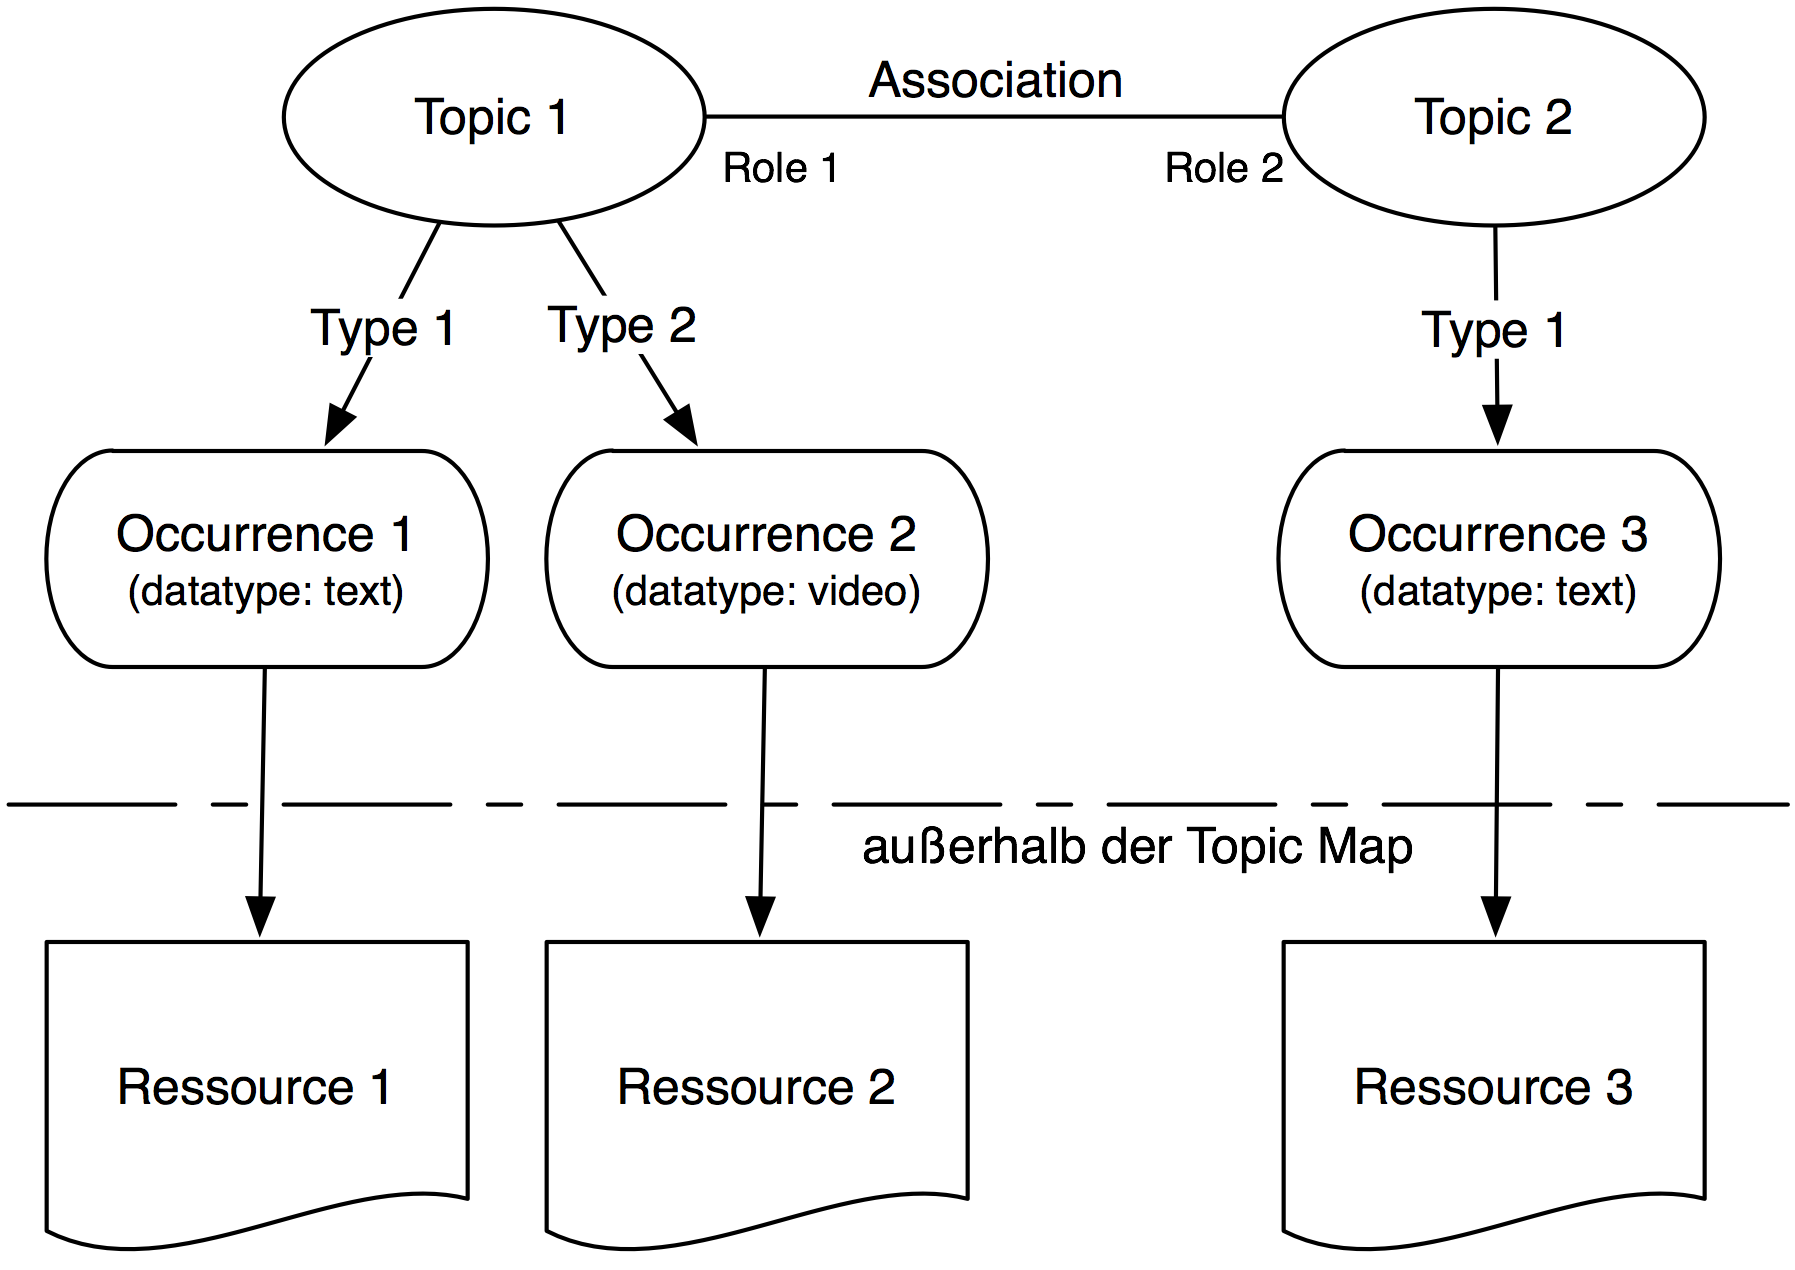
\includegraphics[width=10cm]{img/Persistenz/TMBasic.png}
	\caption{Grundlegende Elemente einer Topic Map}
	\label{fig:img_Persistenz_TMBasic}
\end{figure}

„Topics“ sind stellen Begriffe dar und bilden die Knoten des semantischen Netzes. Ein Topic kann beliebige Information darstellen, repräsentiert aber immer genau ein Phänomen der realen Welt (d.h. zu einem Topic muss es eine Entsprechung außerhalb der Topic Maps geben, die beobachtbar oder beschreibbar ist und auf die die modellierende Person Bezug nehmen will \footnote{„A subject can be anything whatsoever, regardless of whether it exists or has any other specific characteristics, about which anything whatsoever may be asserted by any means whatsoever. In particular, it is anything about which the creator of a topic map chooses to discourse.“ \citep[][S.8]{TMDM08}}). Eine Topic Map ist damit im Sinne von \citet{Stachowiak73} ein diagrammatisches Modell, das einen bestimmten, für den Modellersteller relevanten Ausschnitt der Realität abbildet.

“Associations“ bilden die Beziehungen zwischen Topics ab und stellen damit die Kanten des semantischen Netzes dar. Eine Association verknüpft Topics semantisch miteinander und kann frei mit Bedeutung belegt werden. Die Art der Beziehungen ist also nicht festgelegt und wird wie die Bedeutung der Topics frei gewählt werden. Topics und Associations decken historisch den Bereich der Darstellung von Thesauri ab, in denen Begriffe definiert und zueinanden in Beziehung gesetzt werden. 

Der zweite historische Ursprung von Topic Maps, die Indizes, werden durch das Konstrukt der „Occurences“ abgedeckt. Occurences (“Auftreten“) sind Referenzen aus der Topic Map in die reale Welt. Sie setzen die Topics einer Topic Map in Bezug zu beliebiger referenzierbarer Information (z.B. Dokumente). Im Kontext der eben genannten Indizes, kann eine Topic Map als der mit Querverweisen versehene Index eines Buches verstanden werden, in dem durch die Angabe von Seitenzahlen auf den Text des Buches verwiesen wird. Diese Verweise durch Angabe der Seitenzahlen sind in diesem Zusammenhang die Occurrences.

Die Ansammlung von durch Associations verknüpften und mit Occurrences versehenen Topics bilden eine Topic Map. Darüber hinaus kann in Topic Maps jedoch noch weiterführende Information repräsentiert werden (siehe Abbildung \ref{fig:img_Persistenz_TMFull}), die Gegenstand der folgenden Abschnitte sein werden.

\begin{figure}[htbp]
	\centering
		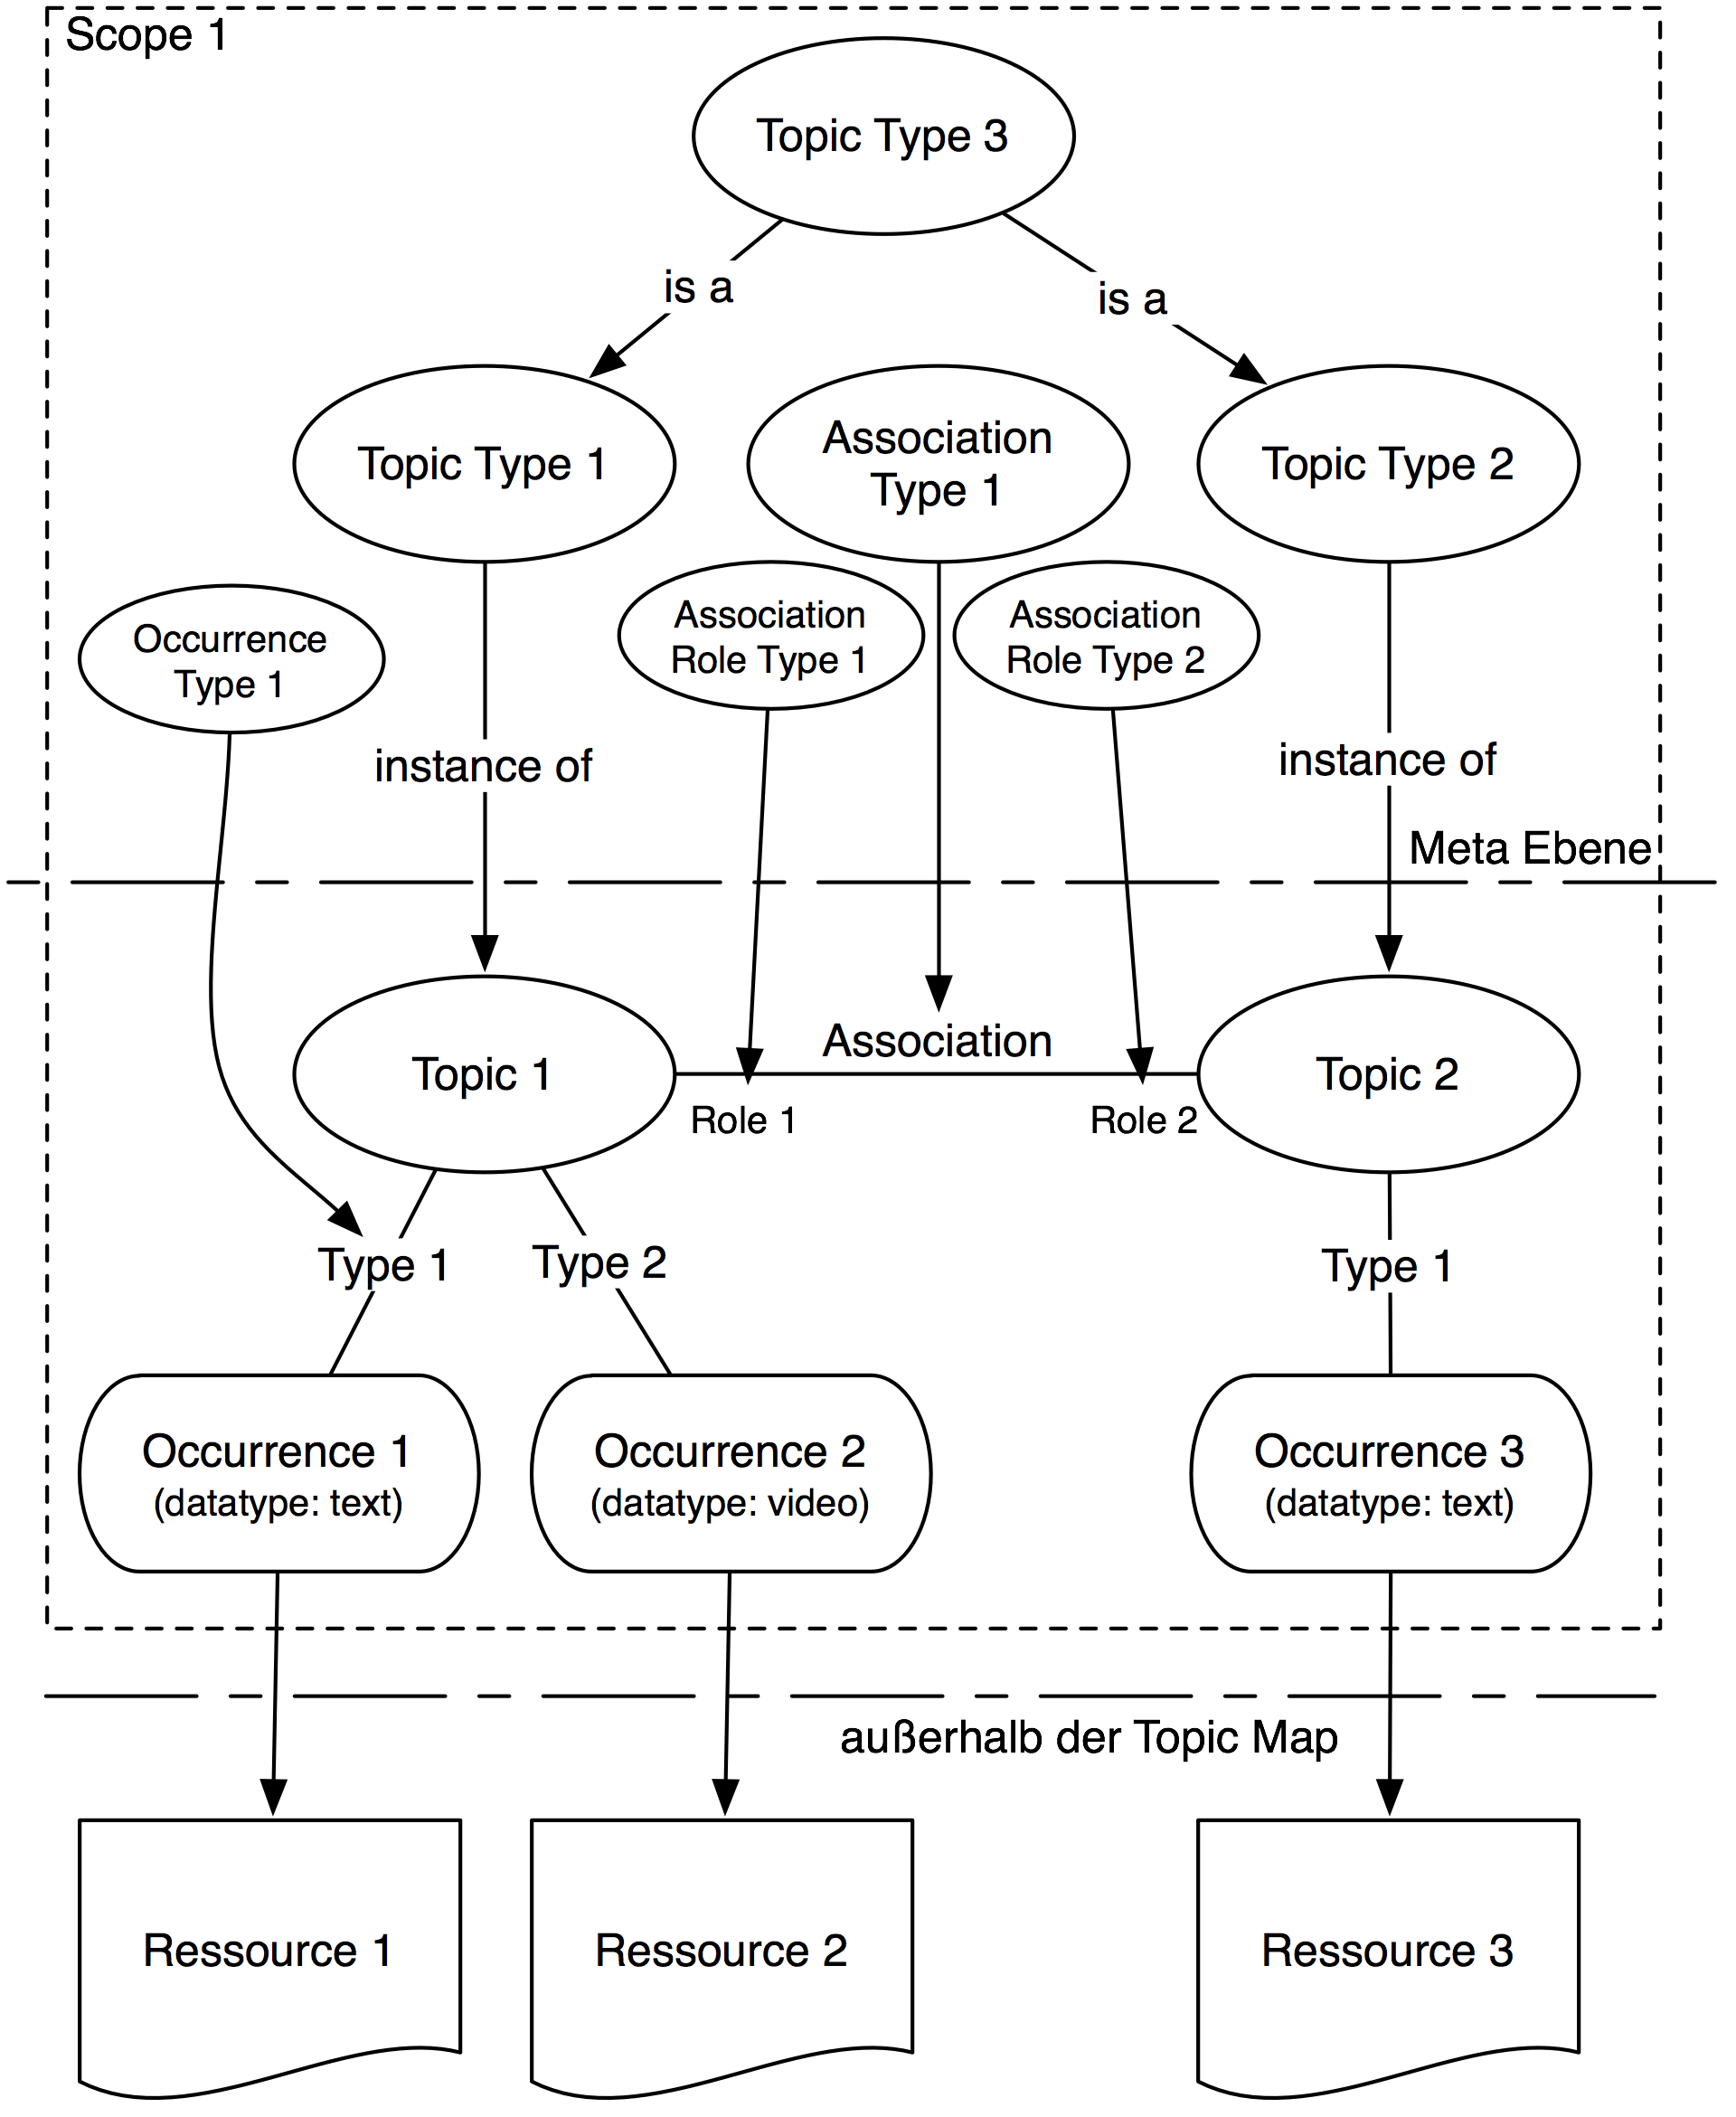
\includegraphics[width=10cm]{img/Persistenz/TMFull.png}
	\caption{Umfassende Darstellung der Elemente einer Topic Map}
	\label{fig:img_Persistenz_TMFull}
\end{figure}

\subsection{Topics, Subjects, Topic Names und Variants} % (fold)
\label{sub:topics_subjects_topic_names_und_variants}

Wie oben bereits beschrieben, repräsentiert ein Topic ein Phänomen der realen Welt in einer Topic Map. Dieses Phänomen der realen Welt, das durch das Topic repräsentiert wird, wird als „Subject“ bezeichnet. In einer Topic Map darf es zu einem Subject nur exakt ein Topic geben, umgekehrt kann ein Topic auch nicht mehrere Subjects repräsentieren, die Zuordnung zwischen Subject und Topic ist also eineindeutig (bijektiv). Im Topic wird dazu exakt ein „Subject Identifier“ registriert, der auf eine Informationsressource verweist, die das Subject für Menschen eindeutig identifizierbar macht (diese Ressource wird als „Subject Indicator“ bezeichnet). Zusätzlich kann ein „Subject Locator“ angegeben werden, der auf das tatsächlich in der realen Welt vorhandene Subject verweist. In Abgrenzung dazu kann es bei der anderen Brücke zwischen realer Welt und Topic Map, den Occurrences, für jeder Topic beliebig viele Zuordnungen geben. Eine Occurrence referenziert auch auf die reale Welt, zeigt aber dort nicht auf das Subject selbst, sondern auf ein dieses Subject beschreibendes Objekt in der realen Welt. Beispielhaft ist dazu in Abbildung \ref{fig:img_Persistenz_SubjectVsOccurrence} dieser Zusammenhang anhand des Topics „Tasse“ dargestellt. Ein anderes Beispiel ist ein Topic „London“, das als Subject die reale Stadt London repräsentiert und dem eine Occurrence zugeordnet werden könnte, die auf eine Landkarte (als in der Realität vorhandene Beschreibung der realen Stadt London) referenziert.

\begin{figure}[htbp]
	\centering
		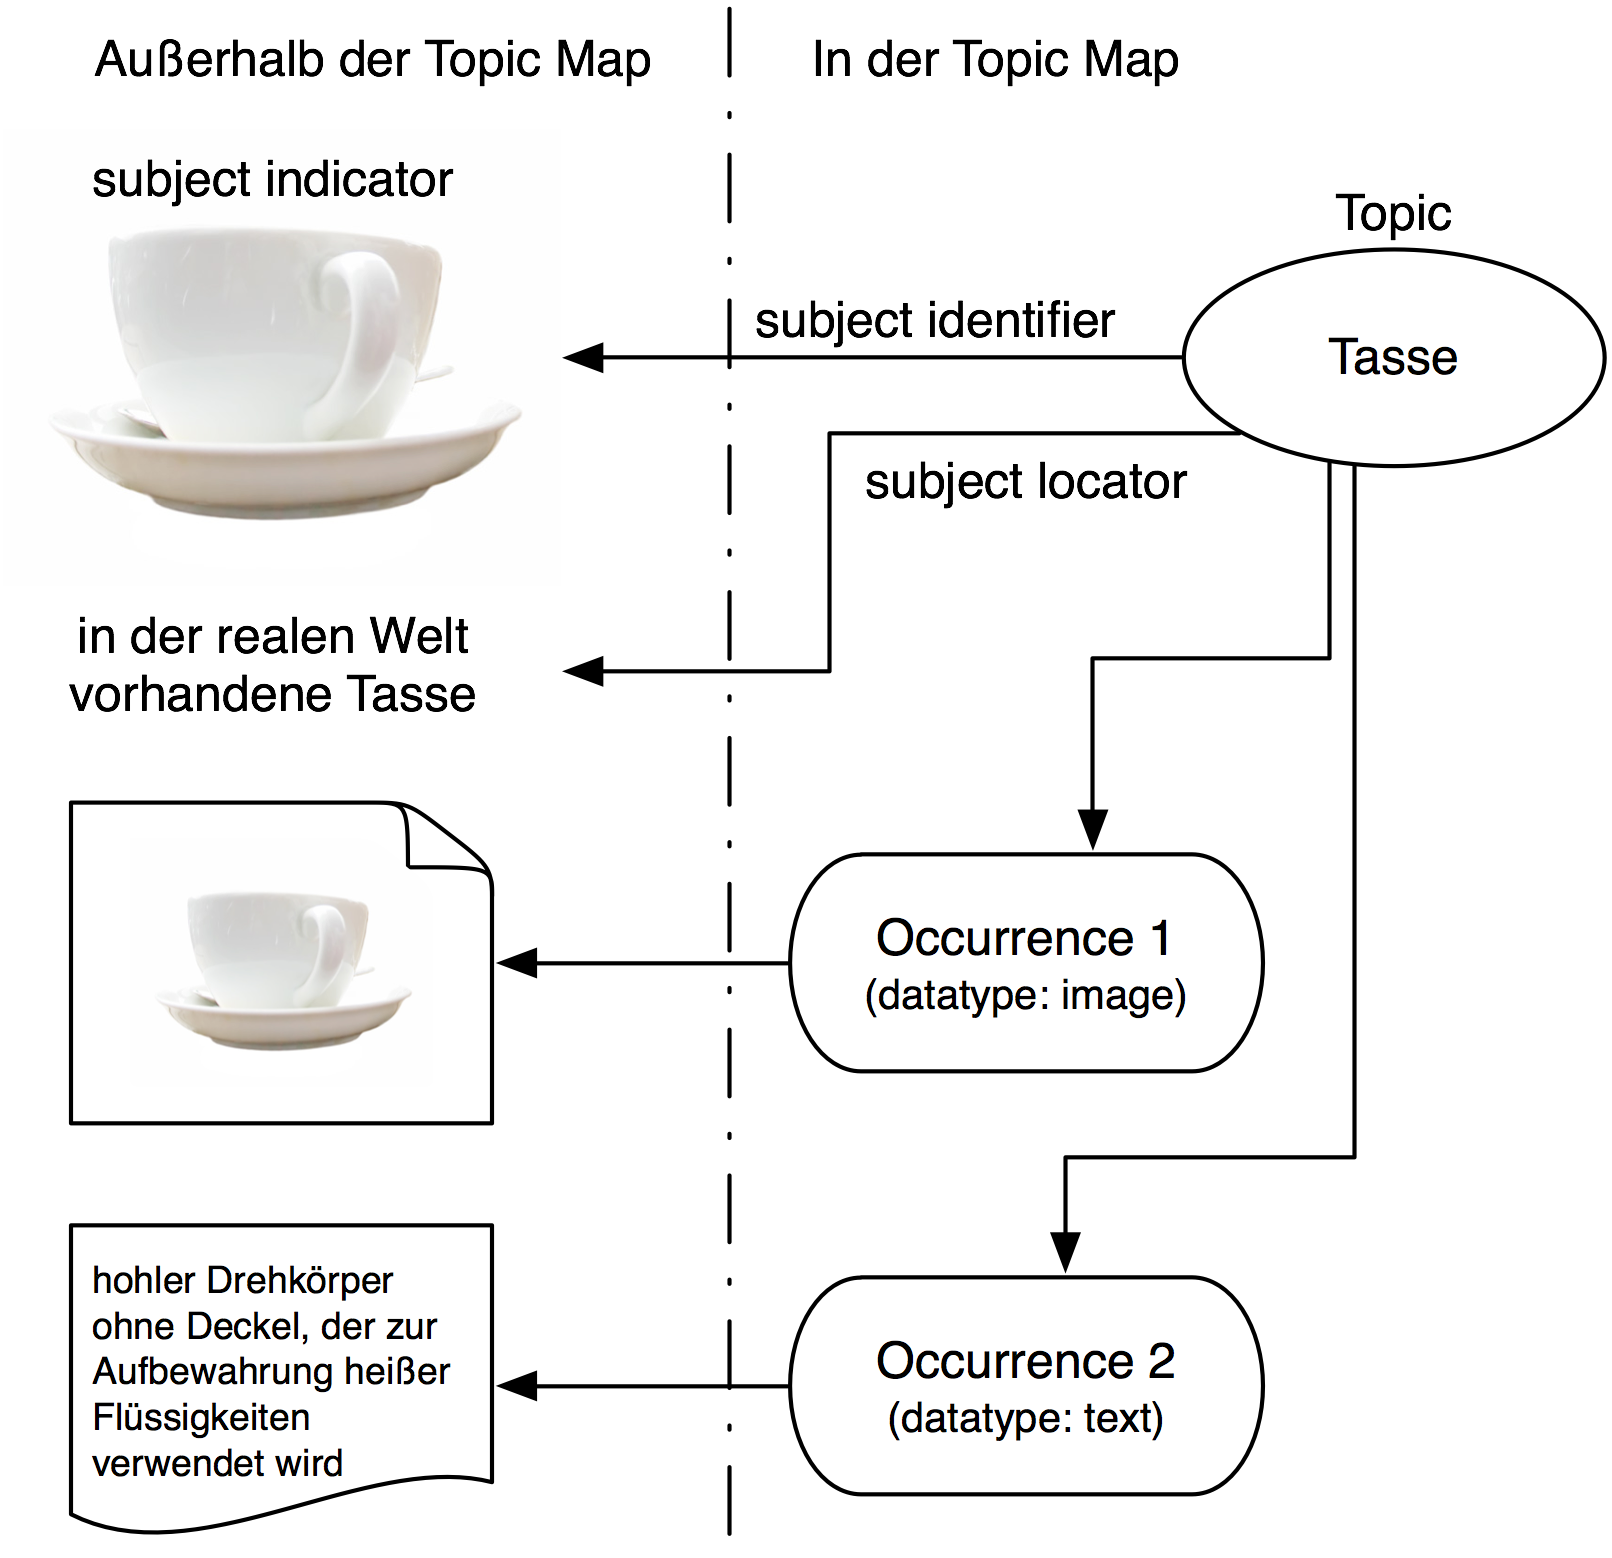
\includegraphics[width=10cm]{img/Persistenz/SubjectVsOccurrence.png}
	\caption{Abgrenzung zwischen Subject und Occurrence in Topic Maps}
	\label{fig:img_Persistenz_SubjectVsOccurrence}
\end{figure}

Bislang wurde vereinfacht ein Topic immer mit einem direkt zugeordneten Namen dargestellt. In einer Topic Map besitzt ein Topic jedoch keinen eindeutigen Namen. Es wird vielmehr durch seinen Subject Identifier eindeutig gekennzeichnet. Dieser ist jedoch nicht unbedingt für Menschen les- und/oder interpretierbar -- der Subject Identifier hat das Ziel, ein Subject für die Verarbeitung durch Software eindeutig zuordenbar zu machen. Für die Bezeichnung eines Topics in einer für Menschen interpretierbaren Form ist die Verwendung von „Topic Names“ vorgesehen (siehe Abbildung \ref{fig:img_Persistenz_TopicNaming}). Topic Names werden immer textuell angegeben und beschreiben das Subject, das durch das betreffende Topic referenziert wird. Durch einen Topic Name soll das Subject für Menschen erkennbar sein, wobei die Zuordnung nicht notwendigerweise eindeutig sein muss (Beispiel: der Topic Name „Jaguar“ kann ein Fahrzeug oder eine Großkatze bezeichnen und ist dementsprechend ein zulässiger Name für zwei unterschiedliche Topics). Einem Topic können beliebig viele Topic Names zugewiesen werden -- es ist so zum Beispiel möglich, eine mehrsprachige Topic Map zu realisieren, in der zu jedem Topic Topic Names in unterschiedlichen Sprachen angegeben werden. 

\begin{figure}[htbp]
	\centering
		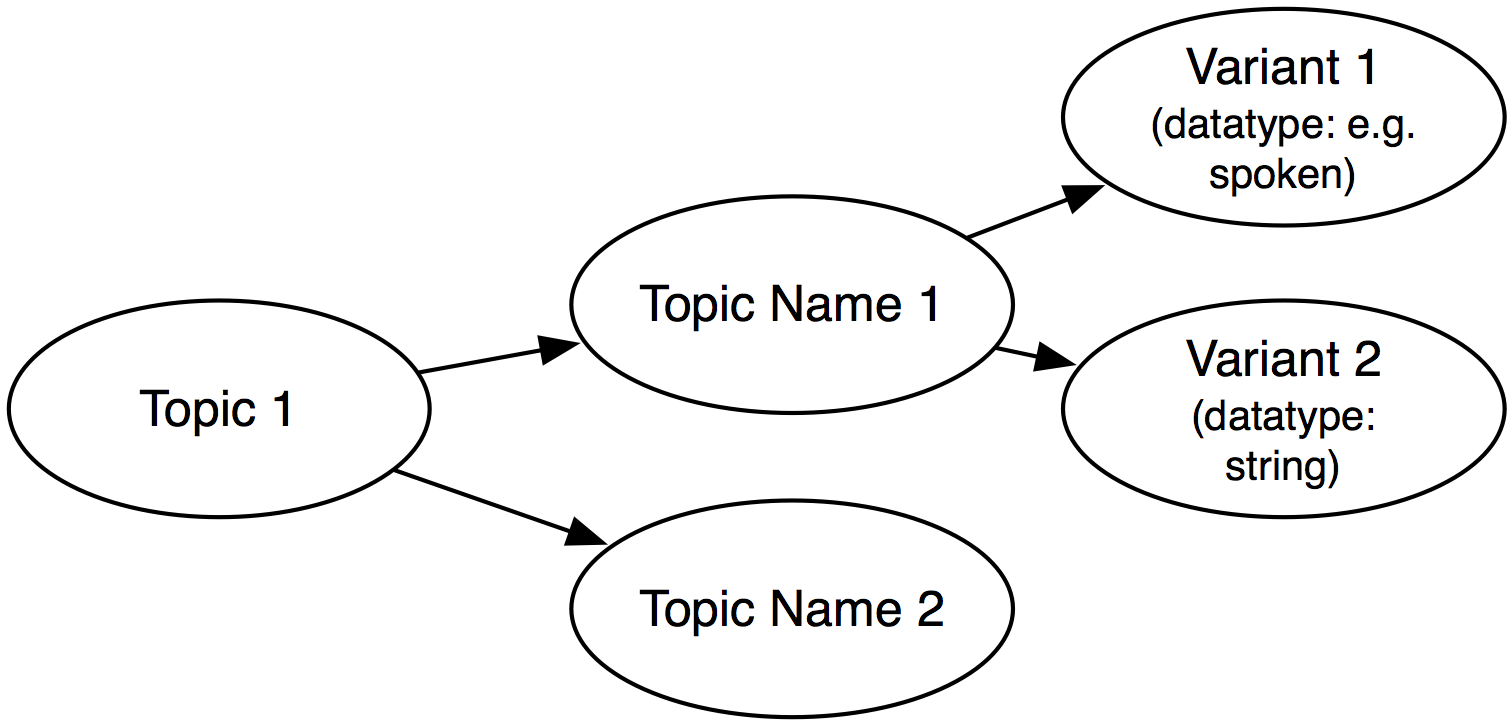
\includegraphics[width=10cm]{img/Persistenz/TopicNaming.png}
	\caption{Benennung von Topics}
	\label{fig:img_Persistenz_TopicNaming}
\end{figure}

Als weitere Detaillierungsstufe können zu jedem Topic Name „Variants“ angegeben werden. Wie durch den Namen angedeutet, handelt es sich dabei um Varianten eines Topic Names, die in bestimmten Zusammenhängen oder für gewisse Anwendungszwecke besser geeignet sein können als der eigentlich Topic Name. Ein Beispiel für eine mögliche Variante ist die Angabe einer gesprochenen Version des Topic Names. Ein weiteres Anwendungsgebiet für Varianten ist die im Standard explizit vorgesehene Angabe eines „Sort Name“ \citep[][S. 18]{TMDM08}, der es erlauben soll, Topic Maps in eine durch diesen Namen vorgegebene Ordnung bringen zu können. Varianten werden durch die Angabe eines dezidiert dafür gewidmeten Topics in deren Scope (siehe Abschnitt \ref{sub:scopes}) als Sort Names gekennzeichnet.

% subsection topics_subjects_topic_names_und_variants (end)

\subsection{Associations und Roles} % (fold)
\label{sub:associations_und_roles}

“Associations“ stellen Verbindungen zwischen den einzelnen Topics einer Topic Map her. Associations haben beliebig viele Endpunkte, mindestens jedoch einen (sind also nicht von vorneherein immer binär sondern können auch unär sein oder mehr als zwei Topics verknüpfen). Eine Associations enthält wie ein Topic nicht unmittelbar einen für Menschen lesbaren Namen. Diese wird durch ein Topic festgelegt, das die Kategorie festlegt, der die Association zuzuordnen sind (siehe Abschnitt \ref{sub:metamodellierung_in_topic_maps}). Diesem Topic kann wiederum mindestens ein Topic Name zugeordnet werden, welcher letzendlich die Benennung der Association festlegt.

Associations werden jedoch nicht direkt mit Topics verknüpft. Um ausdrucksstärkere Verknüpfungen realisieren zu können, agieren „Roles“ als Verknüpfung zwischen Association und den betreffenden Topics. Roles legen die „Rolle“ -- also die Bedeutung -- eines Topics in exakt der betrachteten Association fest. Diese Bedeutung kann generisch sein und zum Beispiel dazu verwendet werden, die per se ungerichteten Associations unabhängig von ihrer konkreten Bedeutung mit einer Richtung zu versehen (zum Beispiel durch die Zuordnung von Roles „Anfang“ und „Ende“) aber auch um die Beziehung semantisch anzureichern (zum Beispiel durch die Zuordnung von Roles „Veranwortlicher“, „Ausführender“ und „Prozessschritt“ in einer Association „durchzuführen“). Die Anzahl der in einer Association referenzierten Roles gibt damit auch die Kardinalität der Association (also die Anzahl ihrer Endpunkte) an. Aus den konkreten Roles wird dann auf die Topics verwiesen, die diese Roles einnehmen bzw. „spielen“ (tatsächlich heißt die betreffende Eigenschaft einer Role „player“). Genau wie Associations werden Roles nicht direkt benannts sondern über ein Topic, das ihre Kategorie bestimmt, mit einer Benennung versehen (Detail wiederum in Abschnitt \ref{sub:metamodellierung_in_topic_maps}).

% subsection associations_und_roles (end)

\subsection{Occurrences und Datatypes} % (fold)
\label{sub:occurrences_und_datatypes}

Wie zu Beginn dieses Abschnitts bereits beschrieben und in den Erläuterungen zur Thematik der Subjects (siehe Abschnitt \ref{sub:topics_subjects_topic_names_und_variants}) angedeutet, bilden „Occurrences“ die Brücke aus der Topic Map in die reale Welt, indem sie auf Ressourcen referenzieren, die in einem beliebigen Zusammenhang mit den jeweiligen Topic stehen. Ein Topic kann beliebig viele Occurrences haben. Anders als bei Associations existieren für Occurrences keine Roles (was auch nur bedingt sinnvoll wäre, da jede Occurrence nur zu exakt einem Topic gehören kann). Die Bedeutung der Occurrence für das Topic kann wie bei Associations über die Kategorie der Occurrence festgelegt werden, die wiederum durch ein separates Topic repräsentiert wird (siehe dazu auch Abschnitt \ref{sub:metamodellierung_in_topic_maps}). Beispielsweise kann eine Occurrence zur Kategorie „Karte“ gehören und so angeben, dass die so klassifizierte Occurrence zum Topic „London“ auf eine Karte des Stadtgebiets verweist.

Zusätzlich zu der Kategorie wird in einer Occurrence auch der Datentyp der Information angegeben, in dem die referenzierte Information vorliegt. Dabei können beliebige URI (Uniform Resource Identifiers\footnote{wie in RFC 3986 definiert und unter http://www.ietf.org/rfc/rfc3986.txt abzurufen}) verwendet werden. Da URIs beliebigen Inhalt haben können, wäre es in obigen Beispiel möglich durch den Datentyp einer Occurrence festzulegen, ob es sich bei der Karte um eine Rastergrafik oder eine Vektorgrafik handelt und so Information über deren möglich Einsatzgebiete zu einzubetten.

% subsection occurrences_und_datatypes (end)

\subsection{Metamodellierung in Topic Maps} % (fold)
\label{sub:metamodellierung_in_topic_maps}

Wie oben bereits mehrmals angedeutet kann in einer Topic Map neben den eigentlichen zu repräsentierenden Informationen (Topics, Associations, Roles und Occurrences) auch Information über die Topic Map selbst eingebettet werden (neben dem Model also auch das Meta-Modell abgebildet werden kann). Die Information umfasst Angaben über die in der jeweiligen Topic Map existierenen Kategorien von Topics, Topic Names, Associations, Roles und Occurrences. Hinsichlich der Repräsentation dieser Information sind zwei Ansätze zu unterscheiden, von denen der erste bei Kategorieangaben von Topics zum Einsatz kommt, der andere bei Kategorieangaben jeder anderen Art von Information. Allen Kategorien ist gemein, dass sie selbst wiederum als Topics repräsentiert werden und auch als solche verwendet werden können. Es ist also möglich, zu einem Topic, das als Kategorie verwendet wird, selbst wiederum eine Kategorie anzugeben, wodurch die Einführung beliebig vieler Meta-Ebenen möglich ist. Außerdem können als Kategorien verwendete Topics ebenfalls wieder mit Associations verknüpft und mit Occurrences versehen werden. Hinsichtlich der Nomenklatur ist noch darauf hinzuweisen, dass Kategorien im Allgemeinen als „Types“ bezeichnet werden, man also von „Topic Types“, „Topic Name Types“, „Association Types“, „Role Types“ und „Occurrence Types“ spricht.

\subsubsection{Topic Types}

Topic Types werden in einer Topic Map durch ein spezielle, im Standard festgelegte Association definiert. Soll einem Topic ein Type zugewiesen werden, muss eine Association der Kategorie „type-instance“ eingefügt werden, bei der das Topic selbst die Role „instance“ einnimmt und dem Topic, das die Kategorie repräsentiert, die Role „type“ zugewiesen wird. Diese Beziehung entspricht einer Konkretisierung eine (abstakten) Kategorie oder Klasse von Topics auf eine bestimmte Instanz, die die Merkmale dieser Klasse trägt. In Abbildung \ref{fig:img_Persistenz_MetaModelExample} besteht eine type-instance-Beziehung (dort als „instance-of“ bezeichnet) zwischen der Kategorie „VW Golf“ und der konkreten Instanz „SR-174 AU“ (also einem Topic, bei dem das amtliche Kennzeichen als Topic Name verwendet wurde). „VW Golf“ fungiert hier also als Topic Type, wobei es selbst ein Topic ist, das sich durch nichts als die eingenomme „type“-Rolle von einem anderen Topic unterscheidet und dementsprechend behandelt werden kann.

Einem Topic können beliebig viele Topic Types zugewiesen werden, indem es in mehr als einer Association die Role „instance“ einnimmt. Es wird so als mehreren Kategorien zugehörig gekennzeichnet. Umgekehrt kann ein Topic Type mehr als einem Topic zugewiesen werden, indem das betreffende den Topic Type repräsentierende Topic die Role „type“ mehrfach einnimmt.

\begin{figure}[htbp]
	\centering
		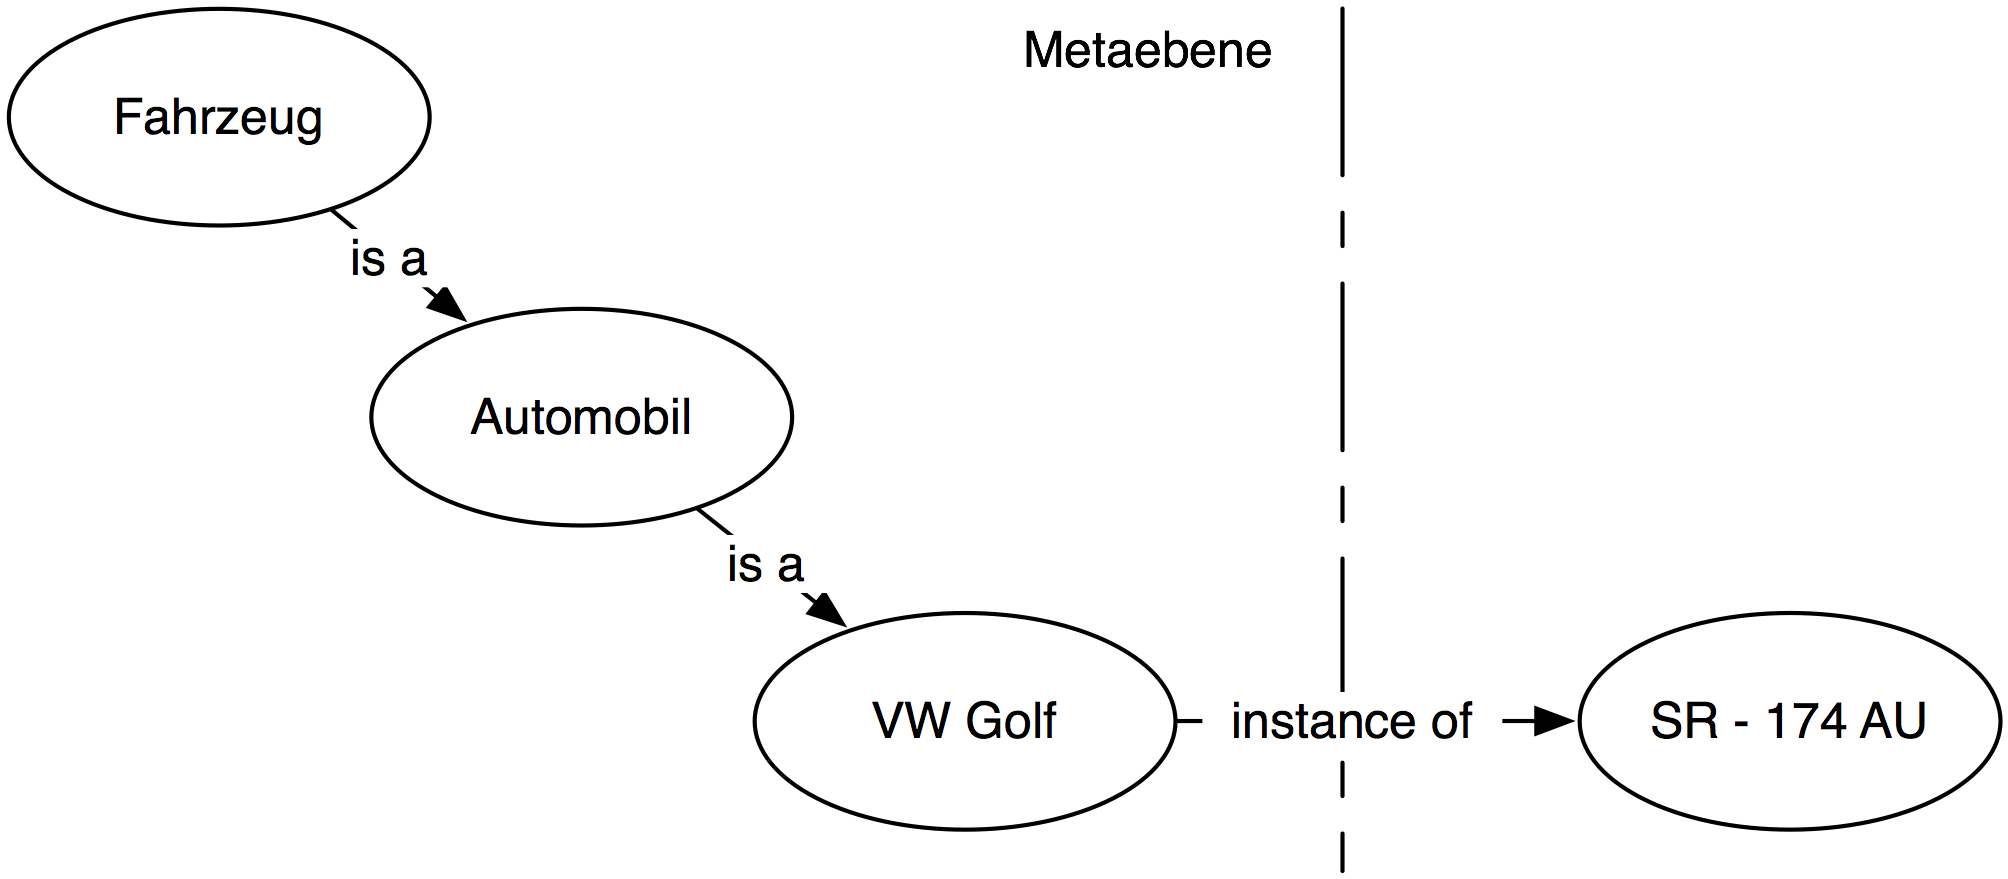
\includegraphics[width=10cm]{img/Persistenz/MetaModelExample.png}
	\caption{Beziehungen in der Metamodellbildung in Topic Maps}
	\label{fig:img_Persistenz_MetaModelExample}
\end{figure}

Auch ist es möglich, Hierarchien von Types zu bilden, in dem einem Topic, das als Topic Type fungiert, selbst wieder ein Topic Type zugewiesen wird. Dieses Konstrukt ist jedoch mit Vorsicht zu gebrauchen, da zur Abbildung der Struktur einer Domäne ein semantisch ähnliches, bei näherer Betrachtung aber eine unterschiedliche Bedeutung tragendes Konstrukt zum Einsatz kommt. Grundsätzlich muss unterschieden werden, ob ein Topic eine konkrete Instanz eines anderen ist oder lediglich eine Spezialisierung darstellt. Im ersteren Fall kommt eine „type-instance“ zum Einsatz, das übergeordnete Topic befindet sich semantisch auf eine anderen, abstrakteren Ebene und stellt eine Kategorie (also einen Topic Type) dar. Im Falle einer Spezialisierung kommt eine „supertype-subtype“-Association zum Einsatz, deren Rollen „supertype“ vom übergeordneten, allgemeineren bzw. „subtype“ vom untergeordneten, spezielleren Topic eingenommen wird. Hier befinden sich beide Topics semantisch auf einer Ebene, keines ist abstrakter als das andere. Der Unterschied liegt vielmehr in der mehr oder weniger konkreten Festlegung der durch die Topics repräsentierten Subjects. So ist wie in Abbildung \ref{fig:img_Persistenz_MetaModelExample} dargestellt das Topic „VW Golf“ ein Subtype des Topics „Automobil“ welches wiederum ein Subtype des Topics „Fahrzeug“ ist. Hier ist erkennbar, dass „Automobil“ insofern eine Spezialisierung von „Fahrzeug“ ist, als dass es im Allgemeinen motorisiert ist und vier Räder besitzt. „VW Golf“ ist wiederum eine Spezialisierung von Fahrzeug, die hinsichtlich der Form der Karosserie, der Anzahl der Türen und anderen Merkmalen mehr spezialisiert. Zwischen keinem der Topics findet jedoch eine Konkretisierung in dem Sinne statt, als dass auf der untergeordneten Seite von einem konkreten, real existierenden Fahrzeug die Rede wäre -- dazu ist die „type-instance“-Beziehung zu verwenden. Die „subtype-supertype“-Beziehung ist transitiv, d.h. dass ein „VW Golf“ nicht nur ein „Automobil“ ist, sondern auch ein „Fahrzeug“. Für „type-instance“-Beziehungen ist diese Eigenschaft nicht gegeben. 

\subsubsection{Andere Types}

Bei allen anderen Types (konkret also Topic Name Types, Association Types, Role Types und Occurrence Types) wird die Kategorie nicht durch eine separate Association abgebildet sondern durch eine im jeweiligen Informationselement enthaltene Referenz auf ein Topic, das als Type fungiert. Die Darstellung der Kategorie-Information ist damit nicht so explizit wie bei Topic Types, wo sich direkt in der Repräsentation der eigentlichen Nutzinformation niederschlägt. Auch semantisch ist sind die hier behandelten Types gegenüber Topic Types insofern eingeschränkt, als das jedem Element exakt ein Type zugeordnet sein muss (der Type kann also nicht leer sein, auch können nicht mehrere Types zugeordnet werden). Wie oben bereits erwähnt sind Topic Types hier flexibler, einem Topic können beliebig viele oder auch keine Topic Types zugeordnet werden. Dies ist aber nur vordergründig eine Einschränkung. Topics dürfen wie oben beschrieben für jedes Subjekt nur einmal existieren. Hat aber ein Subject und damit ein Topic in unterschiedlichen Domänen unterschiedliche Bedeutungen, muss dies über mehrere Topic Types (in Verbindung mit Scopes, siehe Abschnitt \ref{sub:scopes}) abgebildet werden. Alle anderen Informationskategorien in der Topic Map unterliegen nicht dieser Eineindeutigkeitsregel und können bzw. müssen, sollten sie unterschiedlichen Kategorien zuzuordnen sein, auch mehrfach vorhanden sein. Eine Assoziation, die einen anderen Namen trägt (also einer anderen Kategorie angehört) ist beispielsweise nicht identisch mit der ursprünglichen Assoziation, deren Name ebenfalls bereits durch die Zuordnung zu einer Kategorie festgelegt wurde. 

\subsubsection{Modellieren von Einschränkungen}

Der Topic Map Standard erlaubt zwar die Angabe von Metamodellelementen (Types), ermöglicht es aber nicht Regeln anzugeben, anhand derer der semantisch korrekte Aufbau einer Topic Map geprüft werden. Ed ist beispielsweise möglich, einen Association-Type „hat Mitglieder“ zu definieren, der mittels den Roles „Organisationseinheit“ und „Mitarbeiter“ die Zuordnung von Mitarbeitern zu den Organisationseinheiten eines Unternehmens zuzuordnen. Es ist jedoch in der Topic Map nicht möglich zu spezifizieren, das beispielsweise mindestens drei Mitarbeiter zugeordnet werden müssen oder das es in dieser Beziehung nur eine Organisationseinheit geben darf. Weiters kann nicht spezifiziert werden, durch Topics welchen Types die jeweiligen Roles eingenommen werden dürfen -- beispielsweise ist eine Zuordnung von Produktionsmitteln in der Role „Mitarbeiter“ zulässig bzw. kann sie nicht als unzulässig gekennzeichnet werden.

Ist eine derartige semantische Einschränkung bei der Topic Map Erstellung und die Einführung verbindlicher Strukturvorgaben notwendig, so muss dies außerhalb der Topic Map oder durch externe Interpretation spezifischer Topic Map Elemente geschehen. In ersterem Fall kann die noch finalem Zustand vorliegende TMCL (Topic Map Constraint Language, \citep{TMCL08}), eine Regelsprache zur Einschränkung der Repräsentationsmöglichkeiten in einer Topic Map, verwendet werden. Im zweiten Fall können die Metamodell-Elemente (also alle Topics, die als Types verwendet werden) durch zusätzliche Associations verknüpft werden, die semantisch so interpretiert werden, dass sie eine zulässige Kombination von Topics der jeweiligen Kategorie anzeigen.

% subsection metamodellierung_in_topic_maps (end)

\subsection{Statements und Scopes} % (fold)
\label{sub:scopes}

Topic Maps bieten die Möglichkeit, Gültigkeitsbereiche für die in ihnen abgebildeten Informationen zu spezifizieren. Ein Gültigkeitsbereich definiert, in welchem Kontext eine Information gültig ist. Außerhalb dieses Kontext kann über die Gültigkeit keine Aussage getroffen werden. Der Gültigkeitsbereich wird als „Scope“ bezeichnet. Ein Scope kann für jedes „Statement“ in der Topic Map gesetzt werden. Statements sind alle „Aussagen“ über Topics, die in der Topic Map abgebildet werden, nicht aber Topics selbst. Als Statement werden Topic Names, Associations und Occurrences betrachtet. Roles und Variants besitzen keinen Scope, da sie keine direkte Aussage über Topics treffen, sondern nur im Zusammenhang mit Associations bzw. Topic Names existieren, deren Scope sich quasi auf sie vererbt.

Ein Scope für ein Statement wird durch die Angabe eines oder mehrerer Topics festgelegt. Wird kein Topic angegeben, so gilt der „unconstrainted scope“, das Statement ist unbeschränkt gültig. Topics zur Abbildung von Scopes können explizit angelegt werden (z.B. Topics „Deutsch“ und „Englisch“, die Sprach-Scopes ermöglichen, Topics „Tierwelt“ und „Transportwesen“ zur Domänenabgrenzung -- siehe Abbildung \ref{fig:img_Persistenz_Scope}), es ist jedoch grundsätzlich auch möglich, die Gesamtheit der Topics einer Domäne zur Definition eines betreffenden Scopes heranzuziehen (also alle in der Topic Map vorhandenen Topics, die Tiere repräsentieren, als Scope zu verwenden, um den Gültigkeitsbereich „Tierwelt“ abzubilden). Obwohl der Topic Map Standard hier explizit offen bleibt, erscheint jedoch erstere Variante hinsichtlich der Verwaltbarkeit aber auch der semantischen Vollständigkeit wegen als ratsamer (das Konzept „Tierwelt“ käme ansonsten z.B. nicht notwendigerweise vor, sondern wäre nur implizit vorhanden, was eine Auswertung schwierig macht).

\begin{figure}[htbp]
	\centering
		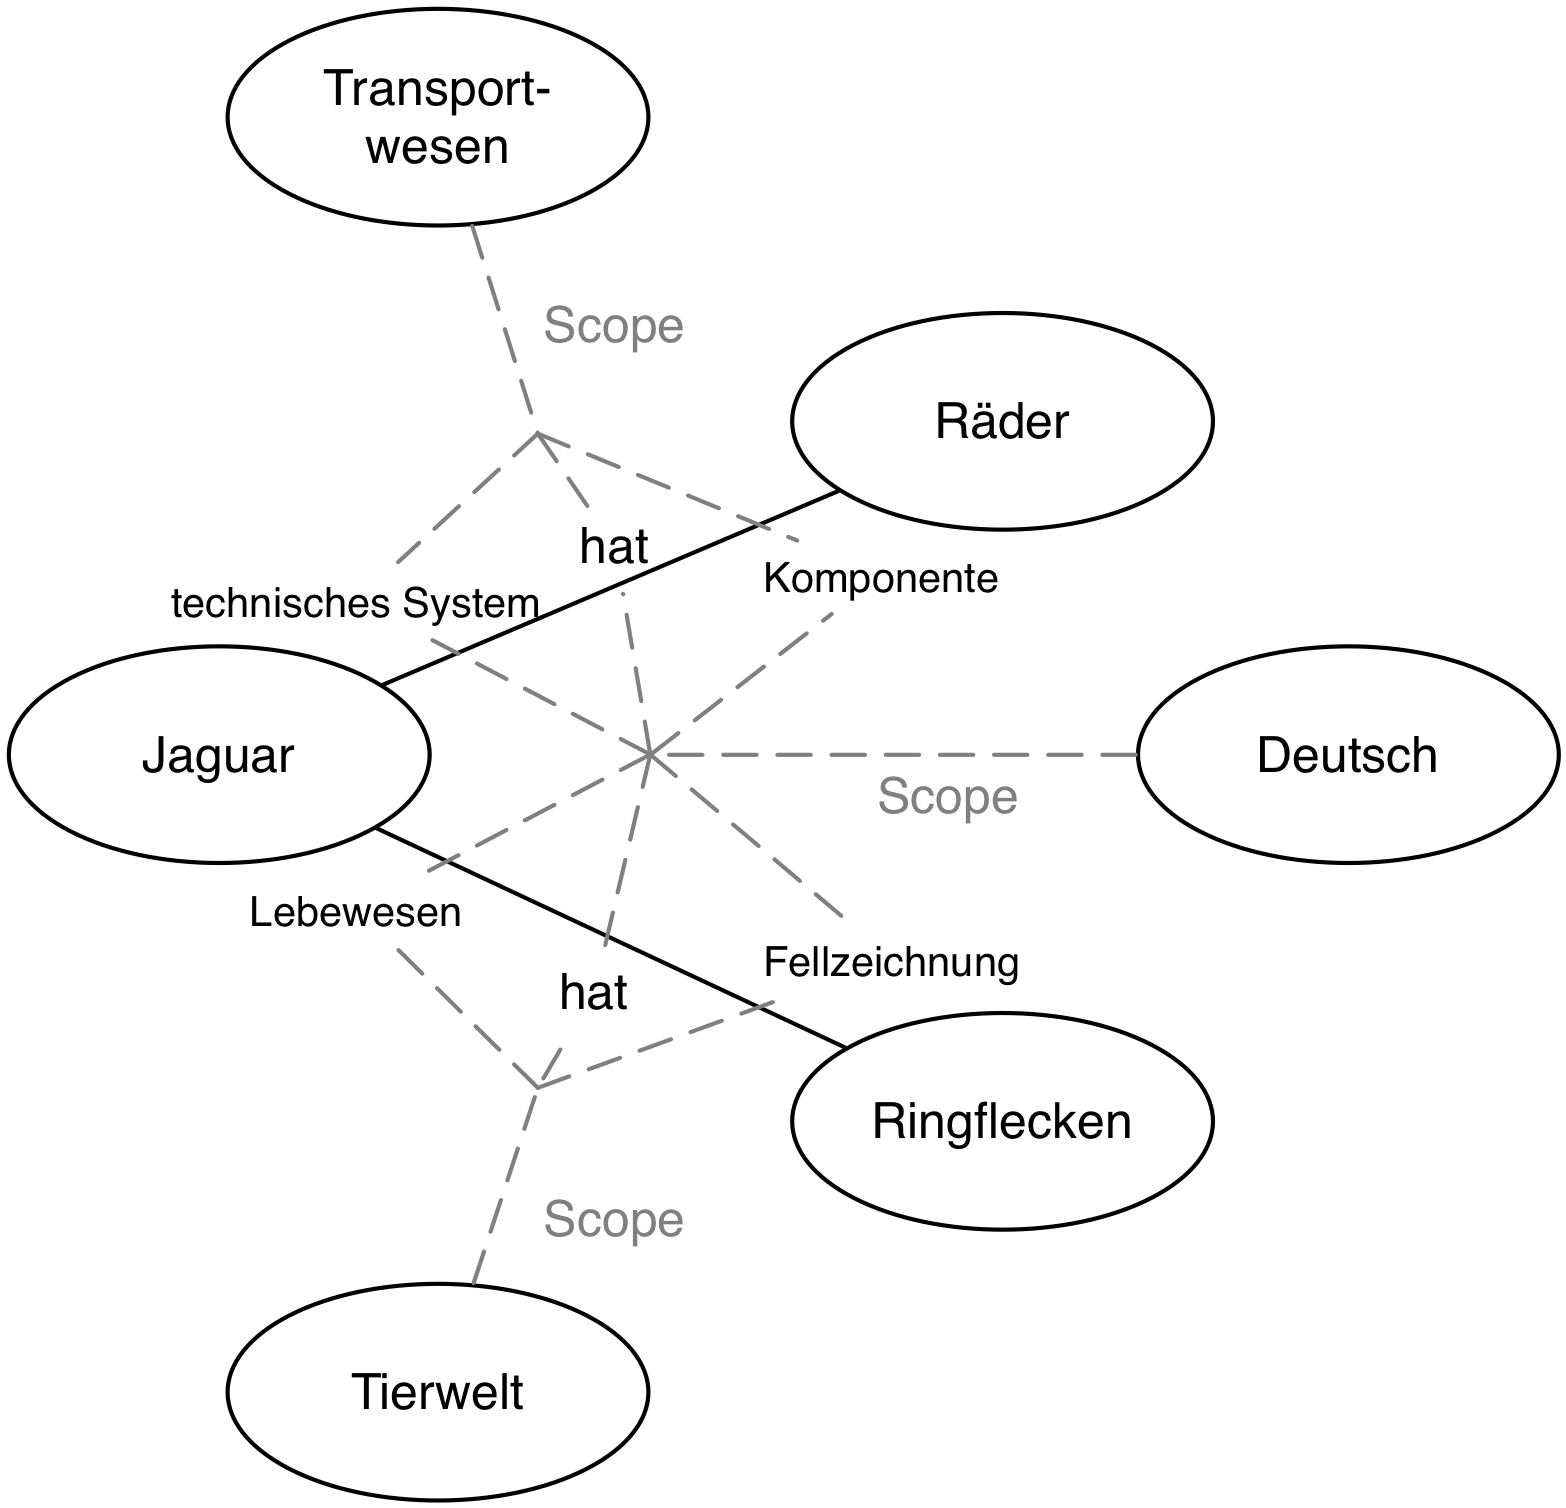
\includegraphics[height=3in]{img/Persistenz/Scope.png}
	\caption{Abbildung von Gültigkeitsbereichen durch Scopes}
	\label{fig:img_Persistenz_Scope}
\end{figure}


Wird mehr als ein Topic angegeben, so bilden alle Topics gemeinsam den Kontext, indem das Statement gültig ist. Bei der Auswertung des Gültigkeitsbereichs müssen also alle angegebenen Topics zutreffen, damit ein Statement gültig ist. Ein Statement dessen Scope die Topics „Tierwelt“ und „Deutsch“ enthält, ist also nur gültig, wenn beide Topics zutreffen (also z.B. zur Filterung ausgewählt wurden). Die gültigen Statements sind also die Schnittmenge jener der Statements, die im Scope „Tierwelt“ und im Scope „Deutsch“ gültig sind (siehe Abbildung \ref{fig:img_Persistenz_Scope}). Die Angabe eines Scopes zu einem Statement, das in beiden Scopes (unabhängig voneinander gesehen) gültig sein soll, ist nicht direkt möglich. In diesem Fall muss das Statement zweimal jeweils unter Angabe eines der beiden Scopes eingefügt werden.

Für Topics selbst kann kein Scope angegeben werden. Das ist hinsichtlich des Topic Maps zugrunde liegenden Konzepts auch nicht sinnvoll, da Topics immer ein Phänomen der realen Welt, das Subject, repräsentieren, das selbst immer vorhanden ist und dessen Gültigkeit bzw. Existenz nicht von anderen Rahmenbedingungen wie anderen Subjects abhängt. Dementsprechend existiert ein Topic immer, lediglich seine Bezeichnung, die Beziehungen zu anderen Topics oder seine Occurrences können abhängig vom einem Scope unterschiedlich sein.
% subsection scopes (end)

\subsection{Reification} % (fold)
\label{sub:reification}

Wie bereits zu Beginn angeführt, können in einer Topic Map beliebige Inhalte abgebildet werden, jegliche Phänomene der realen Welt können durch Topics repräsentiert werden. Konsequenterweise können nun auch Elemente der Topic Map selbst oder sogar die Topic Map ansich durch ein Topic dargestellt werden. Eine derartige selbstbezügliche Abbildung wird als „Reification“ bezeichnet. Der Ausgangspunkt für eine Reification kann ein Statement sein oder eine Topic Map selbst. Topics können nicht verwendet werden, da ein sie repräsentierendes Topic semantisch äquivalent mit dem Ausgangspunkt wäre und damit zwei Topics vorhanden wären, die das gleiche Subject referenzieren. Nachdem die Abbildung zwischen Subject und Topic eineindeutig sein muss, ist ein derartiges Konstrukt nicht erlaubt.

In Abgrenzung zur Types (Association Types, Occurrence Types, \ldots) repräsentiert ein reifizierendes Topic nicht die Kategorie eines Elements sondern das konkrete Element selbst. Es ist so möglich, einem konkreten Element wie einer Association zusätzliche Information hinzuzufügen (etwa eine Occurrence) oder auch eine bestehende Topic Map als Ganzes zu kapseln und durch das sie reifizierende Topic Bezug zu nehmen. 

% subsubsection reification (end)

\subsection{Merging} % (fold)
\label{ssub:merging}

Unter „Merging“ versteht man die Vereinigung zweier voneinander getrennter Topic Maps zu einer gemeinsamen Map. Dabei ist vor allem die Eineindeutigkeitsregel zu beachten, für ein Subject darf also in der resultierenden Topic Map nur ein Topic existieren. Strukturell nicht kritisch, jedoch die Verwendbarkeit einschränkend sind mehrfach auftretende semantisch identische Statements. Soweit möglich, sollten auch diese Duplikate im Merging-Prozess entfernt werden.

Der Topic Map Standard definiert für jede Art von Element Regeln, anhand der festgestellt werden kann, ob zwei Elemente dieser Art identisch sind oder nicht. Ausgangspunkt sind immer die Topics, wobei beim Vergleich ausschließlich vom abgebildeten Subject ausgegangen werden muss. Sind die Subjects identisch, sind im Wesentlichen auch die beiden Topics identisch und können durch eine gemeinsames Topic ersetzt werden. Auf Basis der vereinigten Topic Menge werden nun die enthaltenen Statements verglichen. Damit Statements als identisch erkannt werden, müssen nicht nur ihr eigentlicher Inhalt sondern auch ihre Kategorie (Type), ihr Gültigkeitsbereich (Scope) und das/die ihnen zugeordnete(n) anderen Element(e) identisch sein. Eine Role ist also nur dann mit einer anderen Role identisch, wenn ihr Type, ihr Scope, die Association, der sie angehört und das referenzierte Topic identisch ist. Daraus folgt, das in der Merging-Reihenfolge zuerst die Topics, dann die eigenständigen Statements wie Topic Names, Associations und Occurrences und letztendlich die abgängigen Statements wie Roles und Variants behandelt werden müssen.
% subsubsection merging (end)

% section topic_maps (end)

\section{Abbildung von Modellen auf Topic Maps} % (fold)
\label{sec:abbildung_von_modellen_auf_topic_maps}

Diagrammatische Modelle \citep{Oppl05a} können direkt ohne zusätzliche Transformationen auf Topic Maps abgebildet werden. Derartige Modelle bestehen aus Knoten und Kanten, die Verwendung dieser im konkreten Anwendungskontext ist durch die Modellierungssprache festgelegt. In den folgenden Abschnitten wird nun beschrieben, wie die einzelnen Aspekte eines diagrammatischen Modells auf eine Topic Map abgebildet werden können.

\subsection{Grundlegende Abbildung} % (fold)
\label{sub:grundlegende_abbildung}
Der nahe liegendste Ansatz, um diagrammatische Modelle auf Topic Maps abzubilden, werden nun die Knoten auf Topics, die Kanten auf Associations abzubilden (siehe Abbildung \ref{fig:img_Persistenz_AssociationReification}, Variante 1). Ist in den Kanten mehr Information als die bloße Anzeige der Verbindung von zwei Knoten abgebildet (wie z.B. in \gls{UML} State Charts \citep{Rumbaugh04}, bei denen die zu einem Zustandsübergang führenden Ereignisse inkl. Bedingungen und ablaufende Aktionen in den Kanten repräsentiert werden), so kann es sinnvoll sein, auch die Kanten auf Topics abzubilden, da diesen auf dem Wege der Occurrences zusätzliche Information zugewiesen werden kann (siehe Abbildung \ref{fig:img_Persistenz_AssociationReification}, Variante 2). Associations würden in diesem Fall verwendet, um die Knoten und Kanten des Modells zu verbinden, spielen also in der Repräsentation der Information nur noch ein untergeordnete Rolle. Ein Weg, die direkte Abbildung beizubehalten (indem Knoten auf Topics und Kanten auf Associations abgebildet werden) ist, zur Repräsentation der zusätzlich in den Kanten liegenen Information die Möglichkeit der Reification zu nutzen, den Associations also Topics zuzuweisen, die genutzt werden können, um diese zusätzliche Information zu verwalten (siehe Abbildung \ref{fig:img_Persistenz_AssociationReification}, Variante 3).

\begin{figure}[htbp]
	\centering
		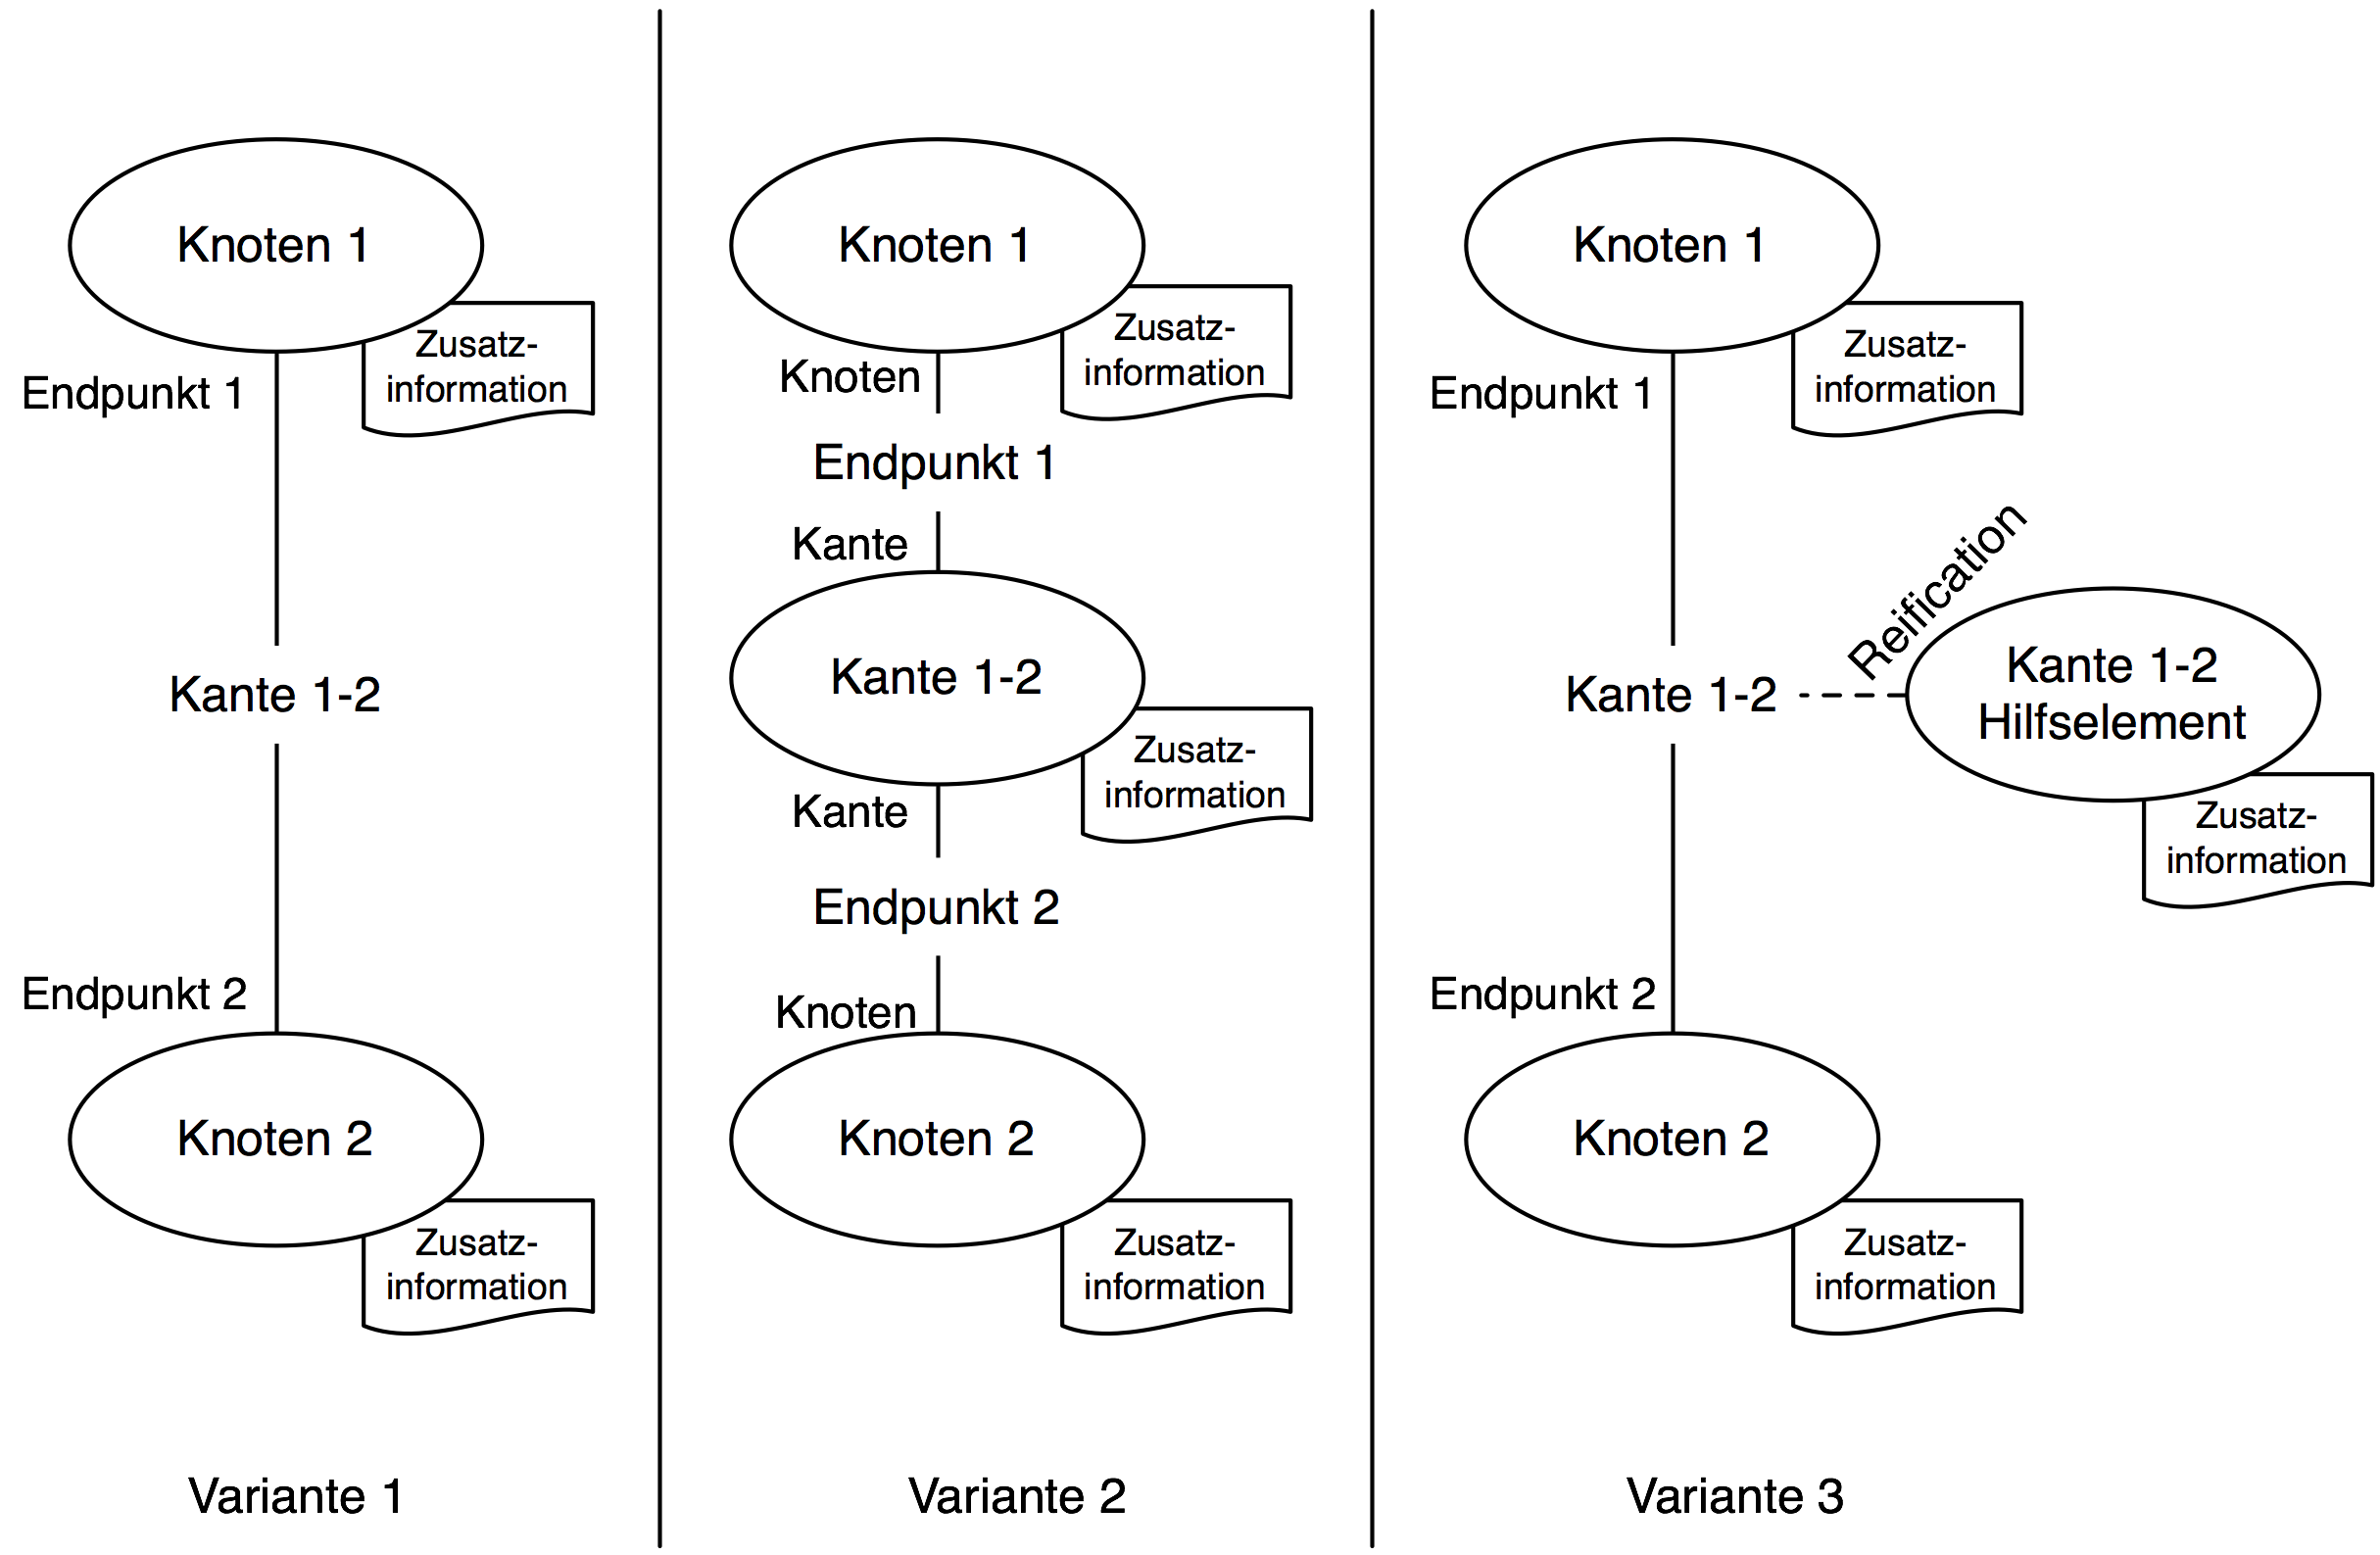
\includegraphics[width=13cm]{img/Persistenz/AssociationReification.png}
	\caption{Abbildung von Modellinformation in Topic Maps}
	\label{fig:img_Persistenz_AssociationReification}
\end{figure}

Die Bedeutung der Knoten des abzubildenden Modells im Kontext einer bestimmten Kante muss in den direkt abbildenden Varianten (in denen Kanten auf Associations abgebildet werden) durch Roles dargestellt werden. In der indirekten Abbildung (bei der Kanten auf Topics abgebildet werden), kann diese Information auch in den Associations repräsentiert werden, die die Topics die Knoten darstellen und jene die Kanten darstellen miteinander verbinden.
% subsection grundlegende_abbildung (end)

\subsection{Abbildung des Metamodells}
\label{sub:abbildung_des_metamodells}
Da Topic Maps von vorne herein nicht auf eine bestimmte semantische Bedeutung der Topics und Associations festgelegt sind, muss auch das Meta-Model der abgebildeten Modellierungssprache mit eingebettet werden. Dies wird in Topic Maps durch die Einbindung von Types ermöglicht. In den nun folgenden Ausführungen wird nur noch auf die direkt abbildende Variante Bezug genommen, da deren Ausdrucksstärke durch die Möglichkeit zur Reification gegenüber dem indirekt abbildenden Ansatz nicht eingeschränkt ist und die unmittelbare Abbildung zu insgesamt kleineren, einfacher zu verwaltenden Topic Maps führt (für eine Kanten wird nur eine Association benötigt, im Gegensatz dazu benötigt der alternative Ansatz ein Topic und mindestens zwei Associations zu Abbildung einer Kante).

Die in der Modellierungssprache festgelegten Arten von Knotentypen (also den eigentlichen Modellierungselementen) werden auf Topic Types abgebildet. Durch die Referenzierung eines einen Knoten repräsentierenden Topics auf diesen Topic Type wird die Bedeutung zugewiesen.

Ebenso wird mit Kanten verfahren. Durch die Einführung von Topics die als Association Types und Role Types fungieren, kann die Bedeutung einer Kante im abzubildenden Modell definiert werden. Dazu wird ein Association Type festgelegt, der die eigentliche Bedeutung der Kante festlegt, die zugehörigen Role Types definieren, wie viele Endpunkte existieren und welche Bedeutung diese haben. Für eine konkrete Kante wird dann eine Association und eine der Anzahl der Endpunkte entsprechende Nummer an Roles erstellt, denen der jeweilige Association bzw. Role Type zugewiesen wird. 

Die Verwendung von Occurrences und dementsprechend die Erstellung von Occurrence Types ist zur reinen Abbildung von diagrammatischen Modellen nicht notwendig. Die Verwendung von Occurrences kann aber sinnvoll sein, wenn aus dem ursprünglichen Modell ebenfalls Ressourcen referenziert werden, die für die weitere Verarbeitung des Modells notwendig sind. Occurrences werden dann im Sinne der Topic Map zur Referenzierung dieser Ressourcen verwendet, wobei sich die zu verwendenden Occurrence Types an der Bedeutung der Ressourcen im abzubildenden Modell orientiert.

Wie in Abschnitt \ref{sub:metamodellierung_in_topic_maps} bereits beschrieben, bietet die Topic Map selbst jedoch keine Möglichkeit, eine explizite Zuordnung zwischen Topic Types, Association Types und Role Types zu definieren, so dass ein in einer Topic Map repräsentiertes Modell auf semantische Korrektheit hin überprüft werden kann. Die einzige ohne zusätzliche Information überprüfbaren Bedingungen sind die Prüfungen, ob alle Knoten und Kanten (also Topics, Associations und Roles) einer Kategorie (also einem Type) zugewiesen  wurden.

Zusätzlich muss also eine externe Möglichkeit geschaffen werden, semantische Korrektheits-Bedingungen zu formulieren und zu überprüfen:
\begin{enumerate}
 \item Zulässige Kategorien von Knoten (Topic Types)
 \item Zulässige Kategorien von Kanten (Association Types, Role Types und eine Zuordnung zwischen diesen, die eine Aussage über die Anzahl und Bedeutung der Endpunkte der Kante zulässt)
 \item Zulässige Verbindungen zwischen Knoten und Kanten (Zuordnung zwischen Endpunkten einer Kantenkategorie und den Knotenkategorien, die diese Endpunkte belegen dürfen -- also eine Zuordnung zwischen Role Types und Topic Types)
\end{enumerate}

Wie bereits oben beschrieben, können derartige Bedingungen innerhalb oder außerhalb der Topic Map formuliert werden. Die Interpretation der formulierten Bedingungen und deren Anwendung auf konkrete Anwendungsfälle muss immer von außerhalb der Topic Map durchgeführt werden. Hier wird der Ansatz der Repräsentation der Bedingungen innerhalb der Topic Map verfolgt, um durch die Übermittlung einer Topic Map nicht nur ein Modell an sich zu übertragen sondern auch jene Information zu liefern, die zur Interpretation derselben notwendig ist.

Die Formulierung der Bedingungen erfolgt auf Ebene der als Types eingesetzten Topics und vervollständigt so das in der Topic Map enthaltene Meta-Modell der Sprache in der das zu repräsentierende Modell erstellt wurde. Die Information über zulässige Knoten und Kanten wird über die Festlegung von entsprechenden Types definiert. Für jeden Typen wird ein Topic eingeführt, das aus dem auf die Topic Map abgebildeten Modell referenziert werden kann. Alle oben notwendigen Zuordnungen zwischen diesen Types werden über Associations abgebildet, die die als Types verwendeten Topics verbinden (siehe Abbildung \ref{fig:img_Persistenz_MetaModelDef}).

\begin{figure}[htbp]
	\centering
		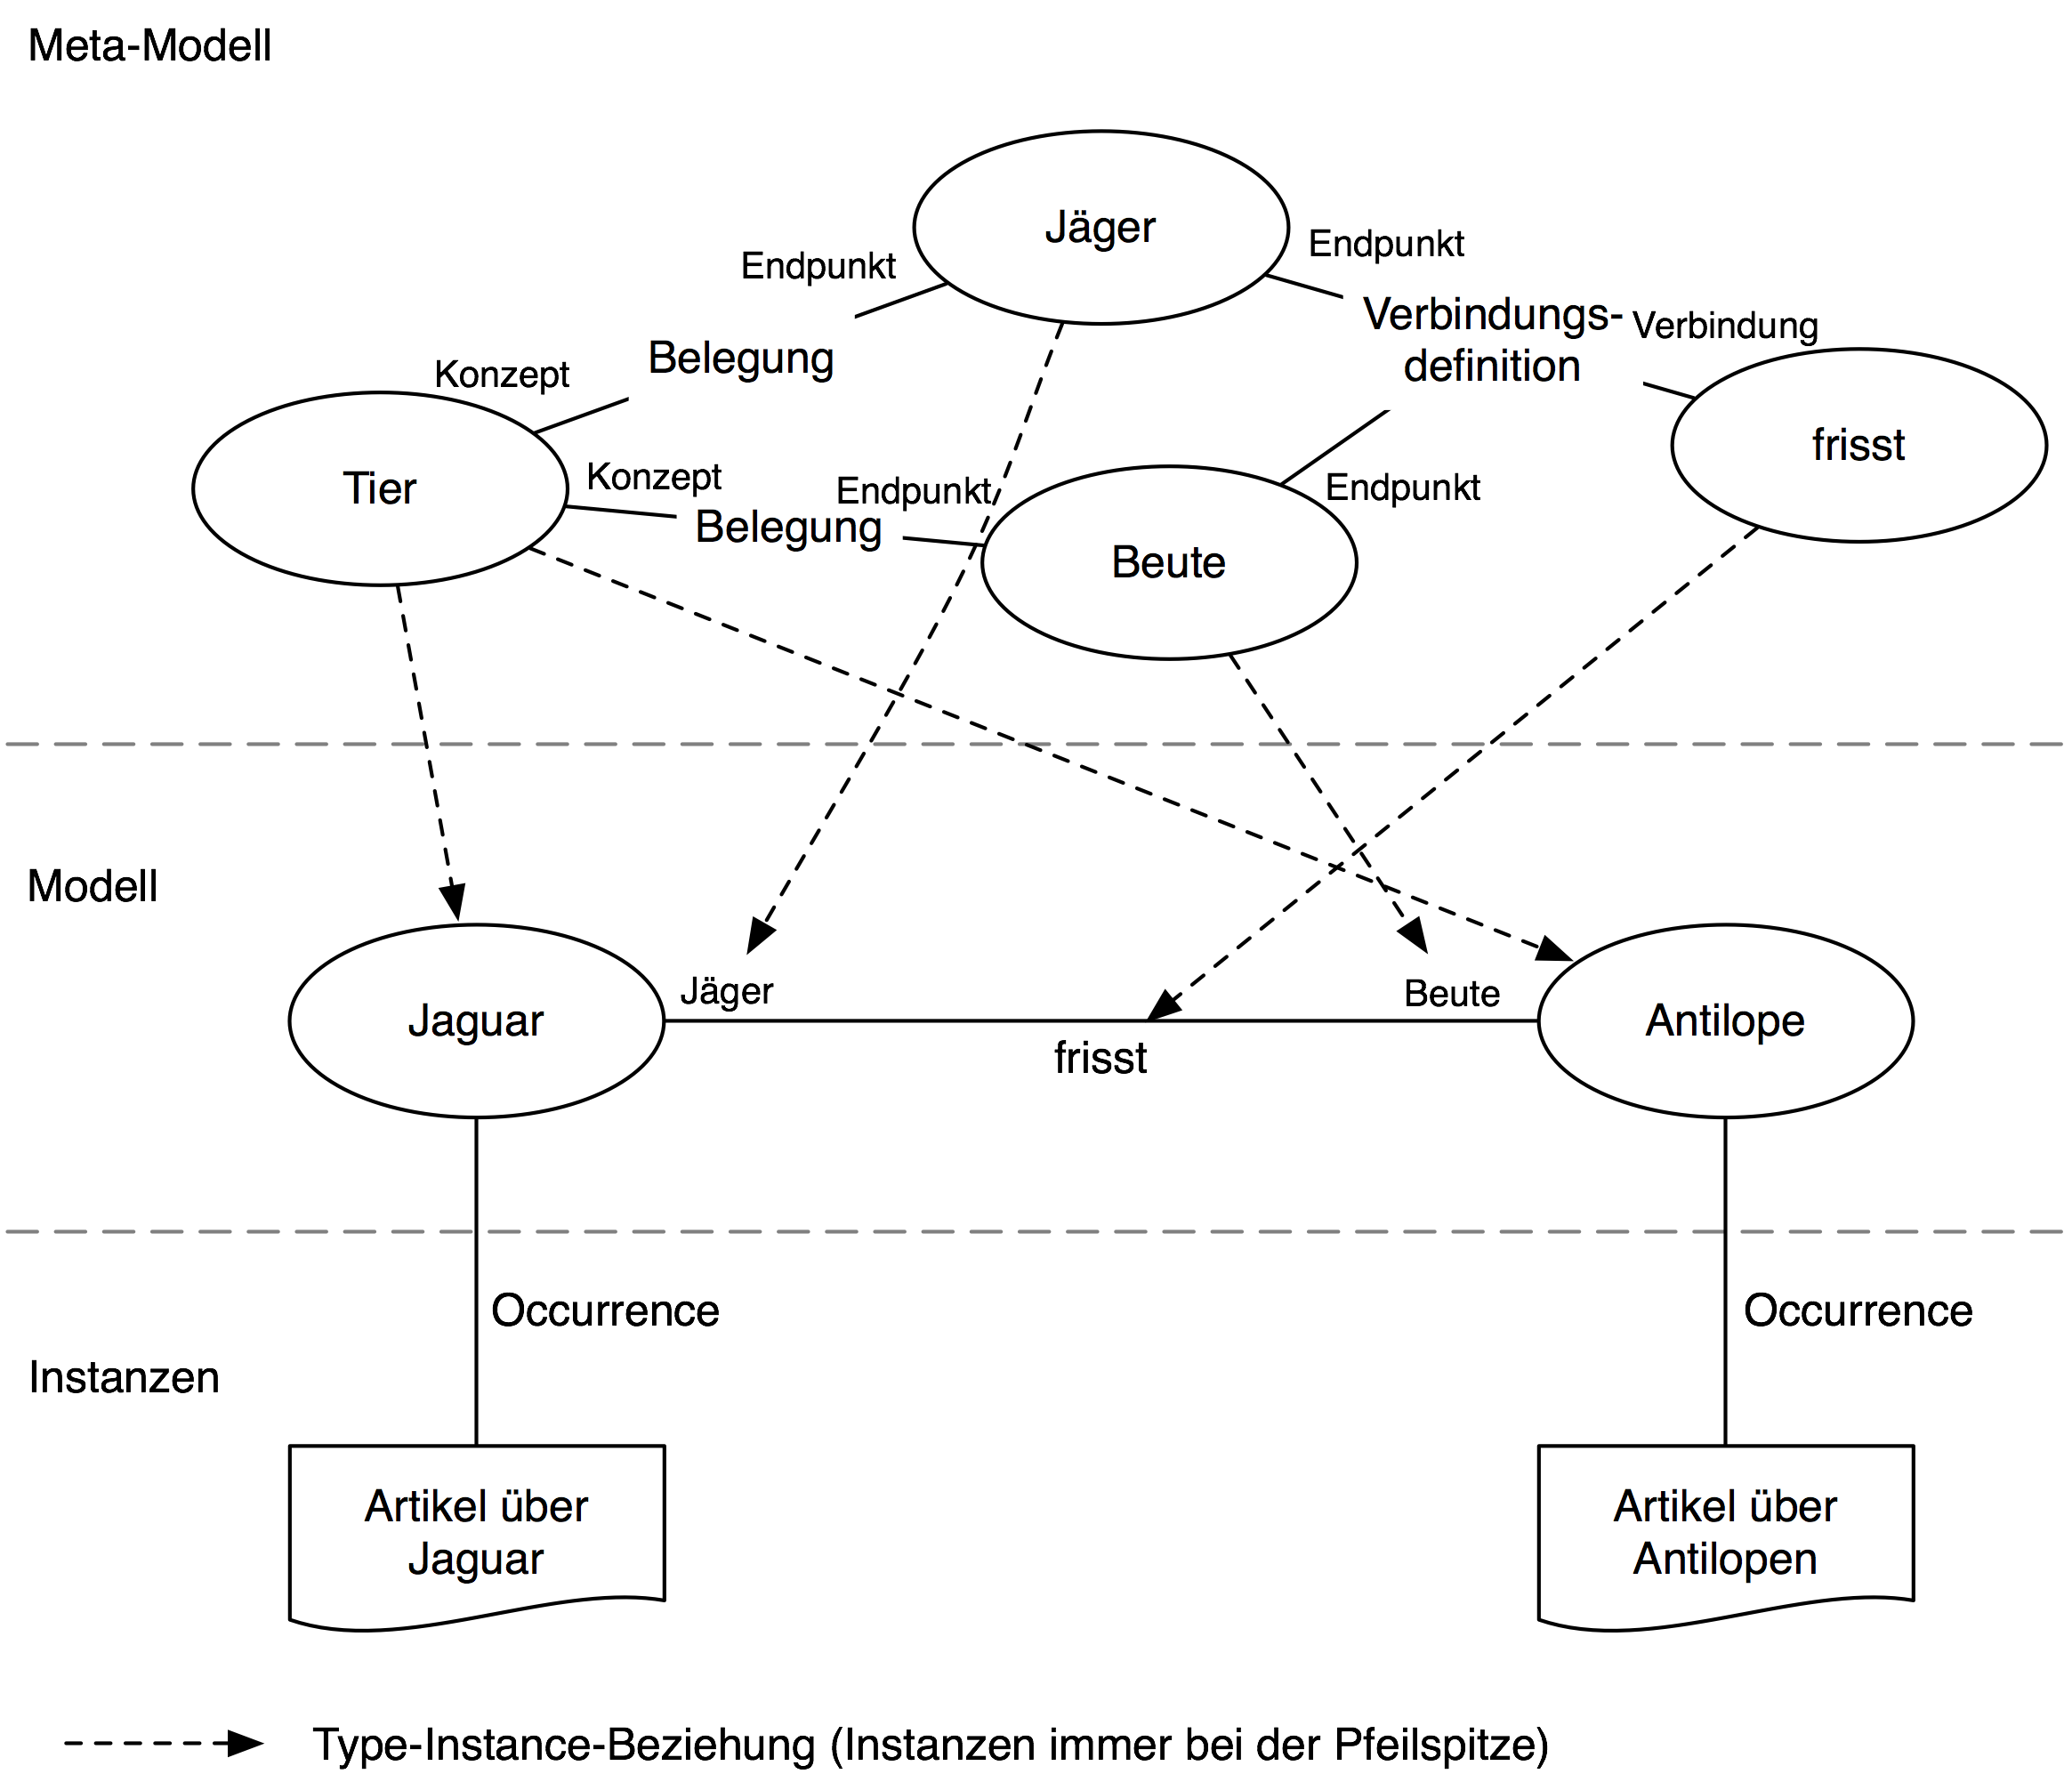
\includegraphics[width=13cm]{img/Persistenz/MetaModelDef.png}
	\caption{Definition des Meta-Models (ohne Kardinalitäten)}
	\label{fig:img_Persistenz_MetaModelDef}
\end{figure}

Die Definition der Kantentypen erfolgt über eine Association mit mindestens drei Roles. 
Eine dieser Roles referenziert den Association Type, die anderen Roles verweisen auf die zu verwendenden Role Types, die zur Beschreibung der Endpunkte der Kante verwendet werden (wovon mindestens zwei vorhanden sein müssen). Die Angabe der Kardinaliät (d.h. wie oft ein bestimmter Endpunkt im konkreten Modell auftreten darf) wird durch eine die jeweilige Role reifizierendes Topic festgelegt.

Ähnlich wird die Zuordnung zwischen Endpunkten und Knotenkategorien realisiert. Zwischen den entsprechenden Topic Types und Role Types werden Associations erstellt, die festlegen, ob eine bestimmte Knotenkategorie einen Endpunkt einnehmen darf oder nicht. Dazu enthält die betreffende Association mindestens zwei Roles, von denen eine auf den Role Type verweist, der den Endpunkt realisiert und eine entsprechende Anzahl von Roles, an die die zulässigen Topic Types (also Knotenkategorien) angebunden werden.

Die eben beschriebenen Abbildungsvorschriften selbst werden ebenfalls in der Topic Map abgebildet. Die Topic Map enthält damit auch das Meta-Meta-Modell das die Elemente die zur Festlegung eines Meta-Models und deren Zusammenspiel festlegt. Eine so definierte Topic Map ist also semantisch vollständig definiert und ermöglicht eine Rekonstruktion eines Modells, das in einer im Vorfeld unbekannten Sprache modelliert wurde, sofern lediglich das Meta-Meta-Modell bekannt ist, dass zur Interpretation der Sprachbeschreibung (Meta-Modell) notwendig ist (siehe Abbildung \ref{fig:img_Persistenz_MetaMetaModelDef}).

\begin{figure}[htbp]
	\centering
		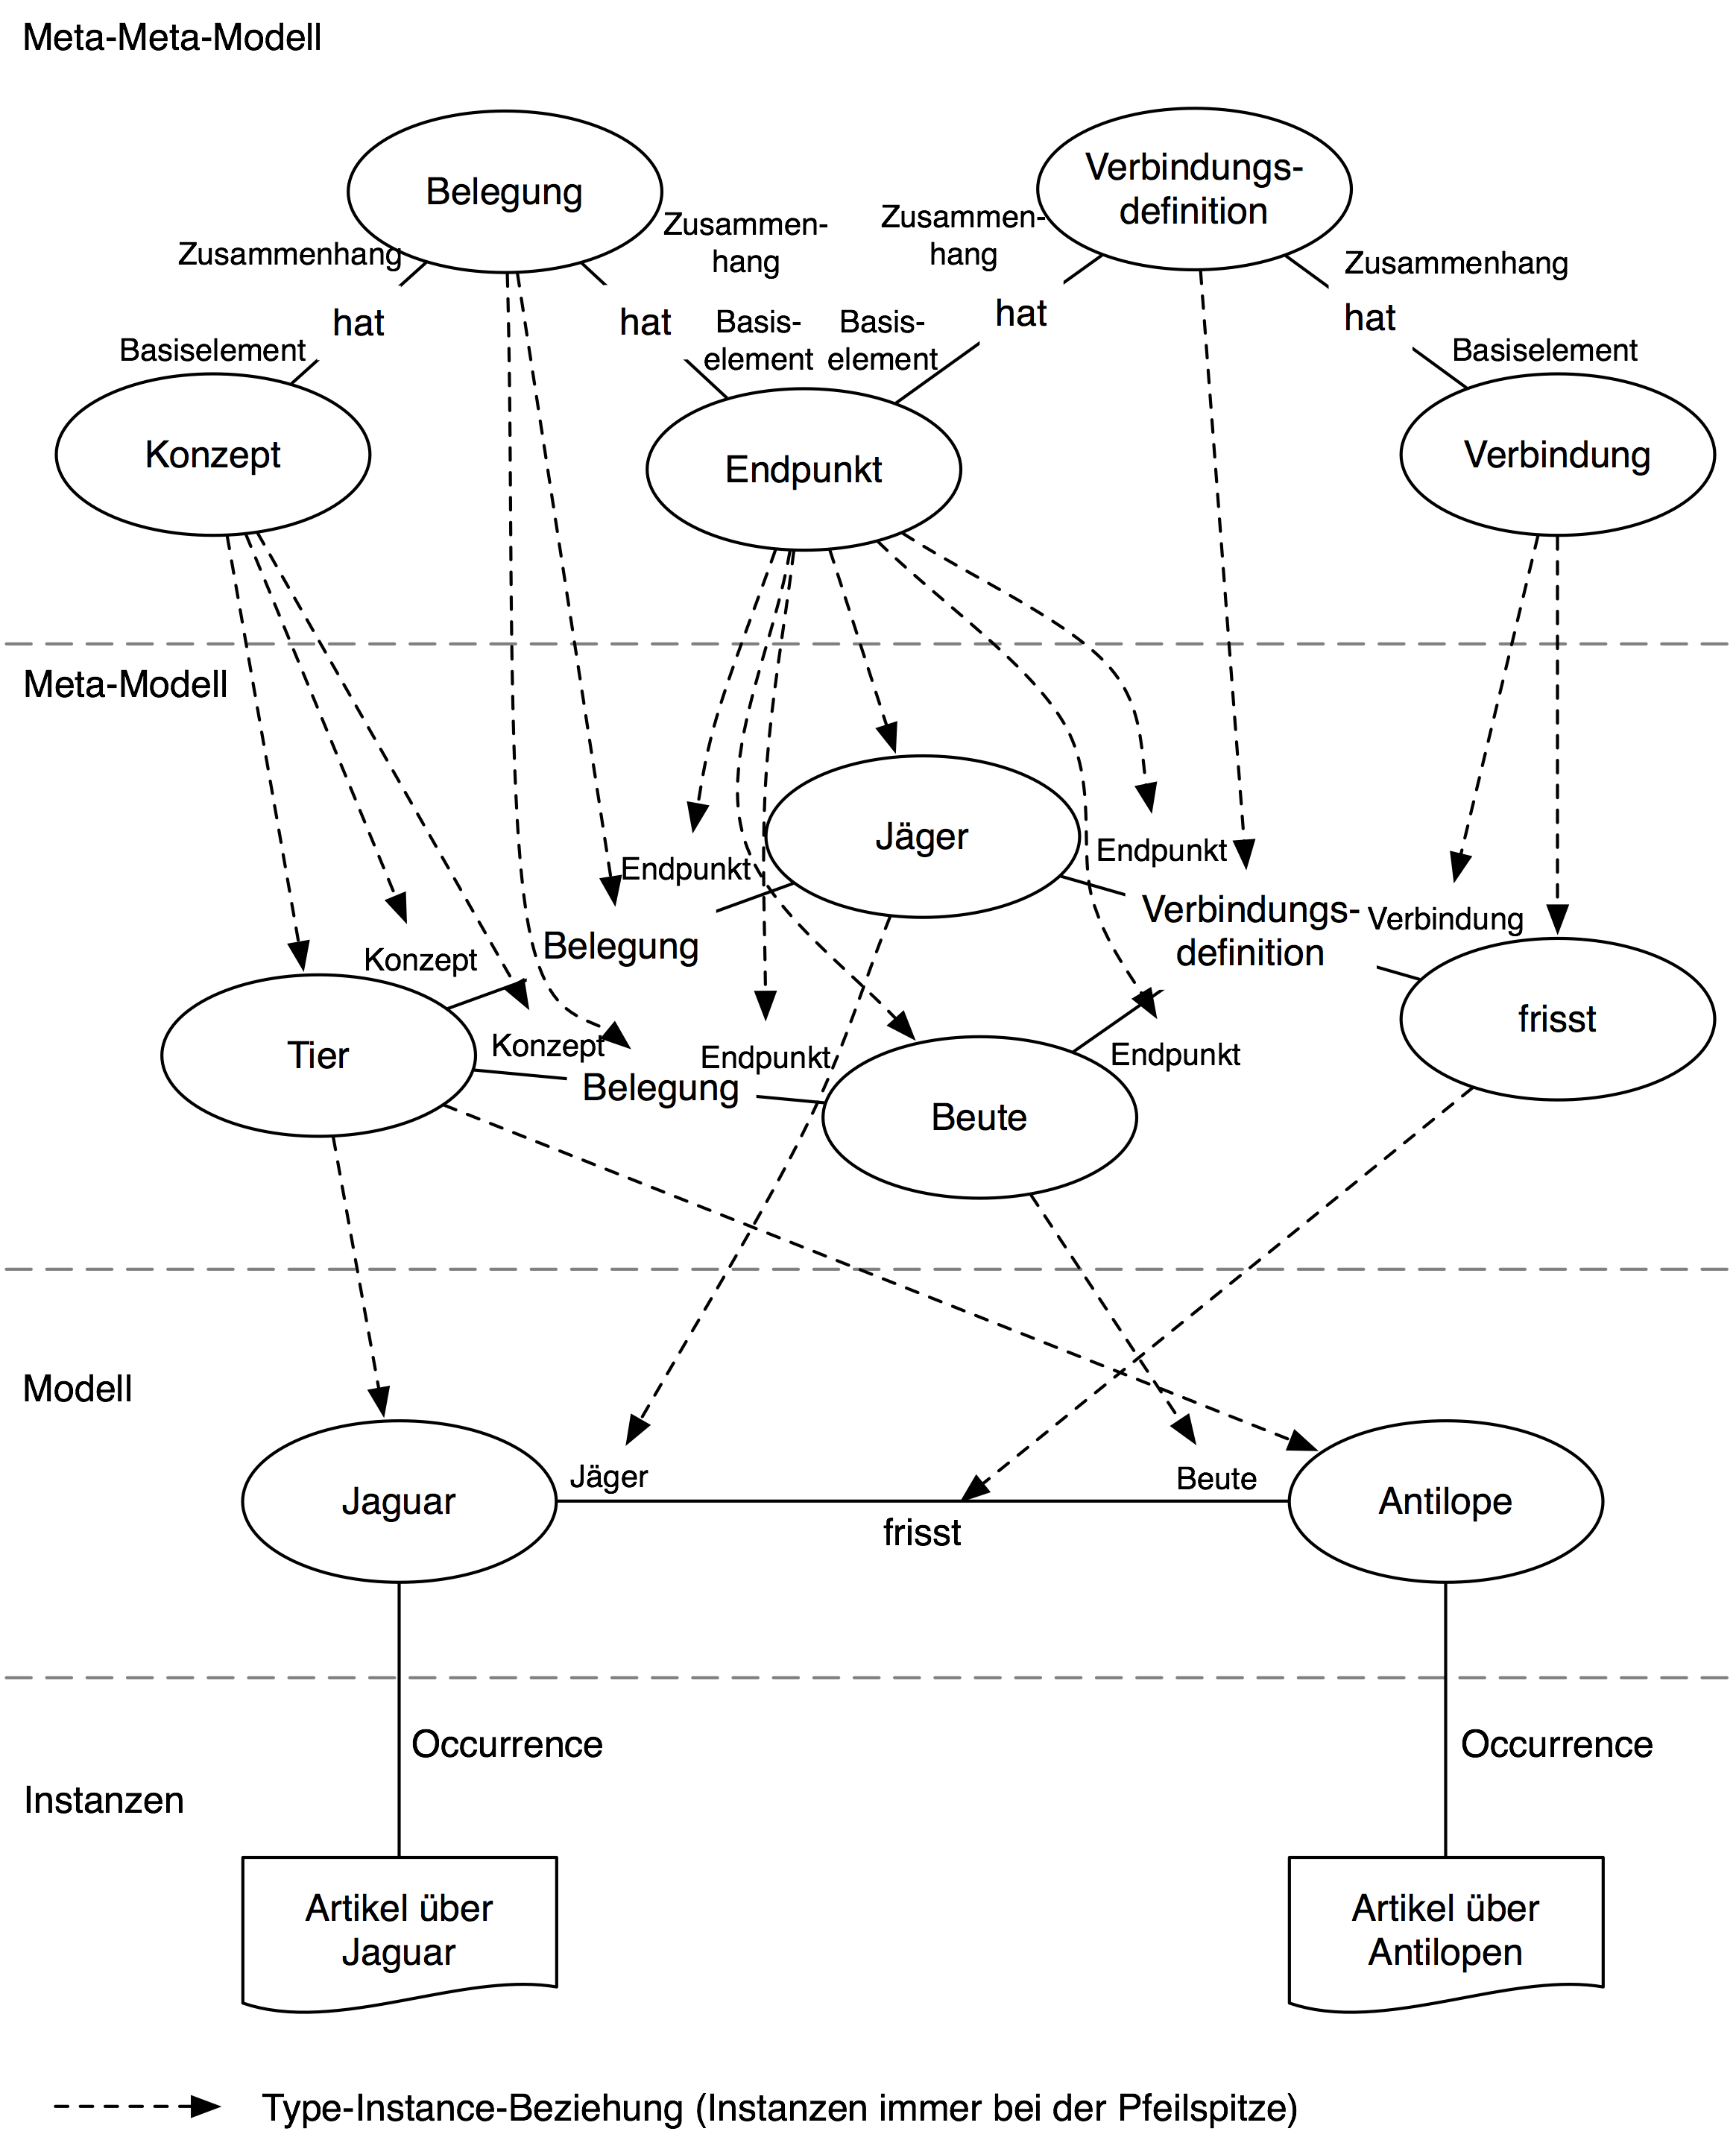
\includegraphics[width=13cm]{img/Persistenz/MetaMetaModelDef.png}
	\caption{Einbindung des Meta-Meta-Modells}
	\label{fig:img_Persistenz_MetaMetaModelDef}
\end{figure}

% subsection abbildung_des_metamodells (end)

\subsection{Abgrenzung von Submodellen}
\label{sub:abgrenzung_von_submodellen}

In einem Modell kann es sinnvoll oder notwendig sein, unterschiedliche Modellbereiche voneinander abzugrenzen. Der Grund für die Abgrenzung kann ein inhaltlicher sein (z.B. eine Partitionierung nach Akteuren bei Aktivitätsdiagrammen \citep{Rumbaugh04}) oder aus dem Modellierungsvorgang heraus motiviert sein (etwa bei der Abgrenzung von Teilmodellen, die durch verschiedene Personen erstellt wurden). Außerdem ist es möglich, in einer Topic Map mehrere Modelle zu repräsentieren, die ebenfalls voneinander abgrenzt werden müssen.

Für diese Abgrenzung bietet sich die Verwendung von Scopes an. Scopes haben zwar keinen Einfluss auf die vorhandenen Topics, wirken jedoch auf die Statements und -- hier relevant -- vor allem auf die die Topics verbindenden Associations. Werden also Scopes eingesetzt, um Teilmodelle voneinander zu unterscheiden bzw. zu trennen, so können die im Moment nicht relevanten Teilmodelle zwar nicht „ausgeblendet“ werden (im Sinne von „temporär vollkommen entfernt“, durch die Entfernung der nicht relevanten Statements sind jedoch nur noch jene Topics untereinander verbunden, die dem aktuell betrachteten Submodell angehören. Ausgehend von einer beliebigen, im Scope gültigen Association oder einem Topic, das bekannterweise dem aktuellen Teilmodell angehört kann so der gesamte relevante Teil der Topic Map erschlossen werden.

Die Realisierung der Trennung zwischen Teilmodellen durch das Ausblenden irrelevanter Verbindungen zwischen Topics birgt einen weiteren potentiellen Vorteil. Werden in einer Topic Map mehrere untereinander zusammenhängende Modelle abgebildet, so wird -- der Grundforderung einer Topic Map nach Eineindeutigkeit entsprechend -- jedes Element nur einmal abgebildet, egal ob es in nur einem Modell verwendet wird oder in mehreren. Durch den Einsatz von Scopes bilden in mehreren Modellen verwendete Elemente automatisch eine Schnittstelle, an der zwischen den Modellen navigiert werden kann. Dieser Vorteil muss in herkömmlichen Modellierungsansätzen mit mehreren untereinander verknüpften Modellen wie der \gls{UML} \citep{Rumbaugh04} oder ARIS \citep{Scheer03} technisch durch explizite Verknüpfung bzw. Referenzierung der äquivalenten Modellelemente in den unterschiedlichen Modeller erzeugt werden. 

Zur Kennzeichnung des Scopes muss zumindest ein Topic verwendet werden. Im Meta-Modell muss festgelegt werden, ob dazu ein Topic eines bestehenden Types verwendet wird oder ein neuer Type eingeführt werden, dessen Topics ausschließlich zum Aufspannen eines Scopes verwendet werden. Dazu wird im Meta-Meta-Modell ein Type „Partition“ eingeführt, der der für alle Elemente des Meta-Modells verwendet werden muss, deren konkrete Instanzen einen Scope im Modell kennzeichnen sollen.

% subsection abgrenzung_von_submodellen}

\subsection{Flexibilisierung der Abbildung}
\label{sub:flexibilisierung_der_abbildung}

Wie in Kapitel XY beschrieben, ist das Meta-Modell von Modellen die im vorgestellten Ansatz entstehen, nicht im vorhinein festgelegt. Die Modellierungssprache -- also das Meta-Modell -- wird während der Modellbildung semantisch definiert und ist damit erst zur Modellierungszeit bekannt. Das Metamodell kann außerdem während der Modellierung erweitert werden, es ist auch möglich, dass sich die Bedeutung bereits existierender Meta-Modell-Elemente ändert.

Für die Persistierung bedeutet dies, dass das Meta-Modell nicht im Vorhinein sondern erst zum Zeitpunkt der Speicherung festgeschrieben werden kann. Außerdem kann die Prüfung auf semantische Korrektheit des Modells ebenfalls nur durchgeführt werden, sobald das Modell definiert ist. 

Um die geforderte Flexibilität bei der Sprachdefinition in Form und Zeitpunkt zu gewährleisten, wurde von \citet{Neubauer08} ein System entwickelt, dass es erlaubt, dynamisch zur Laufzeit Modellelemente zu definieren, die Regeln zu deren Verwendung festzulegen und diese ohne Unterbrechung des Modellierungsvorgangs unmittelbar zu verwenden (wobei auch die Prüfung der semantischen Korrektheit zur Laufzeit adaptiert wird). Die technische Umsetzung dieses Ansatzes wird in Abschnitt \ref{sec:dynamische_metamodelle} beschrieben.

% subsection flexibilisierung_der_abbildung (end)

% section abbildung_von_modellen_auf_topic_maps (end)

\section{Technische Umsetzung der Persistierung von Modellen} % (fold)
\label{sec:technische_umsetzung_der_persistierung_von_modellen}

Die oben beschriebenen Konzepte zur Persisitierung von Modellen wurden wie die übrigen Software-Komponenten des Systems in Java implementiert. Die Basis der Persistenz-Komponente bildet eine Topic Map Engine, die im Rahmen einer Arbeit über flexible Content-Repräsentation vom Autor entwickelt wurde \citep{Oppl07}. Das in \citep{Neubauer08} entwickelte System zur Generierung und Verwendung dynamischer Metamodelle, das bereits in Abschnitt \ref{sub:flexibilisierung_der_abbildung} konzeptuell beschrieben wurde, wird in der Folge hinsichtlich seiner technischen Umsetzung betrachtet. Basierend auf diesen beiden Komponenten wurde die eigentlichen Persistierung implementiert. Der dort verfolgte Ansatz ist Thema des letzten Teils dieses Abschnitts.

\subsection{Topic Map Engine}
Topic Map Engine Persistence Layer

\subsection{Dynamische Metamodelle}
\label{sec:dynamische_metamodelle}

\subsection{Persistierung}
% section technische_umsetzung_der_persistierung_von_modellen (end)


\section{Export graphischer Repräsentationen} % (fold)
\label{sec:export_graphischer_repräsentationen}

Neben der Persistierung der Modelle in Form einer Topic Map ist es auch sinnvoll, die Modelle in deren graphischer Form als Referenz abzulegen. Das hier entwickelte Werkzeug bedient sich der graphischen Ausgabefunktionalitäten, die der Java Klassenbibliothek mit der Version 1.4 hinzugefügt wurden, um das aktuelle Modell in unterschiedlichen Formen als Grafik auszugeben und zur späteren Referenz zu speichern.

\subsection{Ausgabeformen} % (fold)
\label{sub:ausgabeformen}

Zur Speicherung der graphischen Repräsentation eines Modells wird grundsätzlich die Visualisierung verwendet, die auf dem sekundären Ausgabekanal (also dem Bildschirm) zur Anwendung kommt. Beim Export sind nun unterschiedliche Modellaspekte zu berücksichtigen, die je nach intendiertem Verwendungszweck einzeln oder in Kombination in die Ausgabe eingehen können. Diese Aspekte sind im Einzelnen
\begin{itemize}
	\item der aktuell auf der Oberfläche befindliche Modellzustand
	\item die hierarchisch in diesen eingebetteten Submodelle
	\item die Modellierungshistorie, also die Entwicklung des Modells über die Zeit
\end{itemize}

Die Darstellung dieser Aspekte in einer graphischen Repräsentation ist (außer im erstgenannten Fall) insofern komplex, als dass eine beliebig lange zeitliche Abfolge bzw. eine beliebig tief verschachtelte Hierarchie in den zweidimensionalen Raum abgebildet werden muss. Im Falle einer Kombination des zweit- und drittgenannten Aspektes müssen zwei Dimensionen zugleich abgebildet werden, was die Darstellung zusätzlich erschwert.

Der aktuell auf der Oberfläche befindliche Modellzustand wird exakt wie dargestellt in eine Grafik transformiert und als Bild abgespeichert. Zur Abbildung der Modellierungshistorie bietet sich an, die einzelnen gespeicherten Modellzustände chronologisch anzuordnen. Der sich so ergebende Zeitstrahl beginnt links oben und setzt sich von links nach recht und oben nach unten bis in die rechte untere Ecke fort, wo wiederum der aktuelle Modellzustand dargestellt wird. Die zweidimensionale Abbildung des Zeitstrahls erfolgt dabei derart, das sowohl die horizontale als auch die vertikale Ausdehnung des resultierenden Bildes minimal sind (siehe Abbildung \ref{fig:img_Persistenz_ExportHistorie}).

\begin{figure}[htbp]
	\centering
		\includegraphics[width=15cm]{img/Persistenz/ExportHistorie.png}
	\caption{Modellierungshistorie als exportierte Grafik}
	\label{fig:img_Persistenz_ExportHistorie}
\end{figure}

Bei der Darstellung eines Modells mit hierarchisch geschachtelten Teilmodellen bietet sich eine baumartige Darstellung mit dem aktuellen Modellzustand als Wurzelknoten an. Diese ist aufgrund der notwendigen Detaildarstellung der einzelenen Modelle jedoch platzintensiv und kann nur schwer als physisches Dokument abgelegt werden. Deshalb wurde alternativ die hierarchische Strukur auf eine der Darstellung der zeitlichen Modellentwicklung ähnliche Darstellungsform abgebildet. Dabei wird die Hierarchie flach ausgerollt, die Einbettungen zeigen sich durch einen graduell dunkler werdenden Modellhintergrund für tiefere verschachtelte Ebenen. Zusätzlich wird in jedes Submodell farblich abgesetzt auch das jeweilige Containerelement eingeblendet. Die Abfolge der einzelnen Modelle startet mit dem aktuellen Modellzustand als erstem Knoten. Dahinter wird das erste im aktuellen Modell eingebettete Teilmodell angezeigt. Besitzt dieses Teilmodell wiederum eingebettete Teilmodelle, so werden diese in der Folge mit erneut abgedunkeltem Hintergrund dargestellt. Diese Form der Darstellung wird fortgesetztm bis keine weiteren eingebetteten Modelle mehr vorhanden sind. Es folgt (sofern vorhanden) das zweite Submodelle des aktuellen Modellzustandes (mit dem abgedunkelten Hintergrund der ersten Einbettungsebene). Diese Hierarchie wird wiederum bis zu den Endpunkten nach unten verfolgt, es folgt ggf. das dritte Submodell auf der ersten Einbettungsebene. Die sich so ergebende Linie an Modellzuständen wird wie der chronologischen Darstellung der Modellierungshistorie so umgebrochen dass sich sowohl in horizontaler als auch in vertikaler Richtung eine minimale Ausdehung ergibt (siehe Abbildung \ref{fig:img_Persistenz_ExportHierarchie}).

\begin{figure}[htbp]
	\centering
		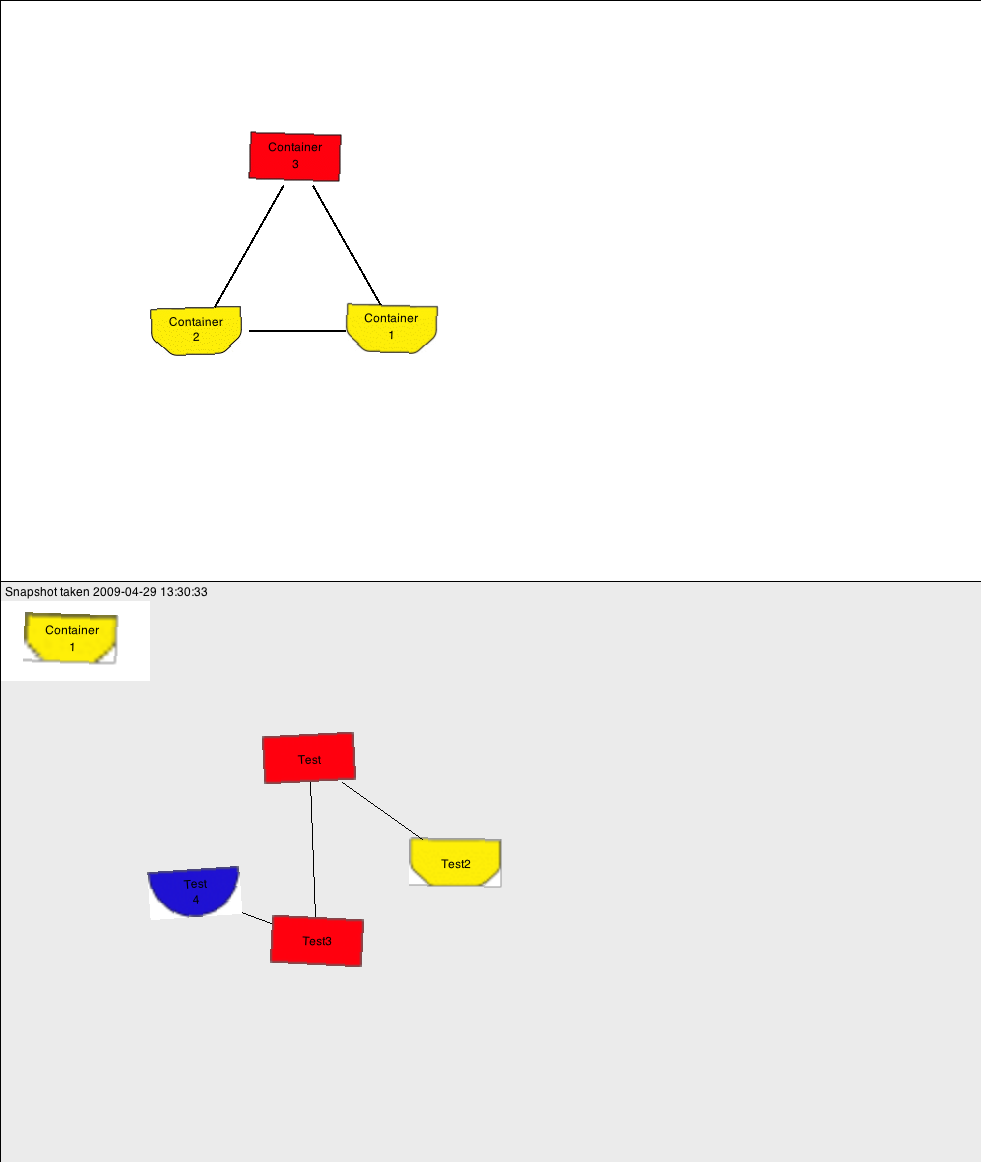
\includegraphics[width=15cm]{img/Persistenz/ExportHierarchie.png}
	\caption{Modell-Hierarchie als exportierte Grafik}
	\label{fig:img_Persistenz_ExportHierarchie}
\end{figure}

In der komplexesten Ausprägung der Darstellung eines Modells als graphische Repräsentation werden sowohl die Historie der Modellentstehung als auch die Hierarchie der eingebetteten Submodelle zugleich dargestellt. Dies erfolgt hier durch die Kombination der beiden eben beschriebenen Ansätze. Die Darstellung der Modellierungshistorie bildet die oberste Ebene der Modelldarstellung. Beginnend mit dem ältesten gespeicherten Modellzustand werden die einzelnen Modelle in der Reihenfolge ihrer Entstehung abgebildet, wobei zu jedem Modellzustand unmittelbar folgend dessen eingebetteten Submodelle ausgegeben werden (deren Entstehung nicht mehr separat dargestellt wird). So ergibt sich eine kombinierte Linie aus chronologischer Modellentwicklung und eingebetteten Teilmodellen. Diese wird wie schon oben mit minimaler Ausdehnung in horizontaler wie vertikaler Richtung auf eine Grafik abgebildet. Die Entwicklung des Modells ist dabei wie gehabt von links oben nach rechts unten zu verfolgen, wobei nur jene Modellzustände mit weißem Hintergrund auf oberster Ebene der Zeitlinie angehören. Alle dunkler hinterlegten Modelle sind Teilmodelle und sind dem nach vorne nächstgelegenen weiß hinterlegten Modell zuzuordnen.

% subsection ausgabeformen (end)

\subsection{Technische Umsetzung des graphischen Exports} % (fold)
\label{sub:technische_umsetzung_des_graphischen_exports}

Zur Umsetzung des graphischen Exports wird auf die mit der Java Plattform in der Version 1.4 eingeführten Klassen zu Verarbeitung von Grafikformaen zurückgegriffen. Diese unterstützen standardmäßig gängige Grafikformate wie \gls{JPEG}, \gls{GIF} oder \gls{PNG}. Im konkreten Fall wurde ein verlustfrei komprimierendes Format gewählt, verlustbehaftete Verfahren wie \gls{JPEG} sind für die hier abzubildenden feinen Strukturen nicht geeignet, da es durch Kompressionsartefakte zu Qualitätsminderungen in der Darstellung von Details kommt.

Die Ausgabe einer Datei im gewählten Grafikformat wird vollständig von der Klasse \texttt{ImageIO} übernommen. Der Schnittstellen-Methode \texttt{write} sind als Parmeter der Dateiname, das Grafikformat sowie ein Objekt der Klasse \texttt{BufferedImage} (allgemeiner: einer Klasse, die das Interface \texttt{RenderedImage} implementiert) zu übergeben, dass die eigentlichen Bilddaten enthält.

Das \texttt{BufferedImage}-Objekt kann durch einen Methoden-Aufruf mit der graphischen Repräsentation einer Klasse, die von der Java \gls{AWT}-Klasse \texttt{Component} abgeleitet ist, befüllt werden. Da alle graphischen Komponenten des JHotDraw-Frameworks Subklassen eben dieser Klasse sind (inklusive der Zeichenoberfläche selbst), können diese durch einen Aufruf ihrer \texttt{paint}-Methode in ein ausreichend großes \texttt{BufferedImage} (bzw. dessen \texttt{Graphics}-Objekt) geschrieben werden.  

In den aus mehr als einem Teilmodell bestehenden Ausgaben (also der Historie, der hierarchischen Darstellung der Teilmodelle oder der Kombination dieser beiden Fälle) muss das Bild aus den graphischen Repräsentationen der einzelnen Teilmodelle zusammengesetzt werden. Dazu werden (im Falle der hierarchischen Teilmodelle rekursiv) die logischen Modelle erzeugt und bereits in der korrekten linearisierten Darstellungsform in einem \texttt{Vektor} gespeichert. Die einzelnen logischen Modelle werden dann in graphische Repräsentationen umgewandelt und in je einem \texttt{BufferedImage} gespeichert. Diese werden in der Folge so zusammengesetzt, dass die horizontale und vertikale Ausdehung der Gesamtfläche minimal ist.

% subsection technische_umsetzung_des_graphischen_exports (end)
% section export_graphischer_repräsentationen (end)

\section{Zusammenfassung} % (fold)
\label{sec:persistierung_zusammenfassung}

% section persisitierung_zusammenfassung (end)
% chapter persistierung (end)


% part umsetzung (end)

% \part{Umsetzung}
% \begin{context}
% In diesem Kapitel wird das entwickelte Werkzeug beschrieben. Es baut auf den Inhalten des vorgehergehenden Kapitels "Design" auf bildet die Basis für die Überprüfung der in den Einleitung definierten Ziele in den folgenden Kapiteln, die sich mit der Evaluation beschäftigen.
% \end{context}
% 
% \begin{structure}
% Dieses Kapitel beginnt mit einem Überblick über das Gesamtsystem und stellt konzeptuell dar, wie die im Kapitel "Design" identfizierten Funktionalitäten zur Umsetzung der Anforderungen umgesetzt wurden. Der zweite Teil widmet sich der entwickelten Hardware und stellt deren Grundstruktur und Besonderheiten dar. Im dritten Teil wird die Softwarearchitektur vorgestellt und auf die wesentlichen zur Umsetzung verwendeten Software-Frameworks und deren Einsatz näher eingangen.
% \end{structure}
% 
% \begin{contribution}
% In diesem Kapitel wurde das in der Einleitung geforderte Werkzeug beschrieben und dessen Entwicklung beschrieben. Das Werkzeug wurde so entwickelt, dass die Anforderungen zur Unterstützung expliziter "Articulation Work" möglichst erfüllt werden, die im ersten Teil dieser Arbeit theoriegeleitet aufgestellt wurden. Die tatsächliche Unterstützungsleistung, die das Werkzeug bietet, wird in den folgenden Kapiteln untersucht. 
% \end{contribution}


\newpage
\textcolor{white}
.
\textcolor{black}
\newpage

\cleardoublepage

\part{Evaluierung} % (fold)
\label{prt:evaluierung}

\chapter{Untersuchungsdesign} % (fold)
\label{cha:untersuchungsdesign}

Die Evaluierung des in der vorliegenden Arbeit beschriebenen Werkzeuges wurde entsprechend der in Kapitel \textbf{XY} vorgestellten konzeptuellen Zusammenhänge mit Fokus auf unterschiedliche Gesichtspunkte durchgeführt. Die beiden grundlegenden Untersuchungsfragen sind
\begin{itemize}
	\item Unterstützen Werkzeug und Methode Articulation Work?
	\item Ermöglichen und unterstützen die Teilwerkzeuge des Modellierungstisches Articulation Work?
\end{itemize}
Die erste Frage setzt im oberen Bereich der Argumentationskette an (\textbf{Bild einfügen}) und untersucht, ob Articulation Work bei Einsatz des Werkzeugs tatsächlich auftritt bzw. ob diese unterstützt wird. Die zweite Frage geht wiederum von der Unterstützung von Articulation Work aus, betrachtet hierbei jedoch den Beitrag der vorhandenen Teilwerkzeuge und zielt auf die Untersuchung der Übereinstimmung zwischen intendierter (bzw. aus den Anforderungen ableitbaren) und tatsächlicher Einsatzgebiete ab. Die diesen Fragen zugrunde liegenden Annahmen und die jeweiligen Ansätze zur Messung werden in den nächsten beiden Abschnitten behandelt. Der letzte Abschnitt dieses Kapitels beschreibt dann die konkrete Planung der Untersuchung und die im Einzelnen durchgeführten Untersuchungs-Phasen. 

\section{Frage 1 – Unterstützung von Articulation Work} % (fold)
\label{sec:frage_1_unterstützung_von_articulation_work}

Axiom 1:
Erfolgreiche Articulation Work zeigt sich an der Production Work (-> Ref. Strauss)

Axiom 1,5:
Erfolgreiche Production Work zeigt sich an der Zielerreichung (-> Erfolg) (-> Ref. Fujimura)

Axiom 2: 
(Geschäfts-)Erfolg steht in direktem Zusammenhang mit funktionierender Interaktion (-> Ref. 

Messung:
Die Unterstützung der Articulation Work kann an Ihren Auswirkungen auf die Production Work gemessen werden, dort im speziellen an der Qualität der Interaktion ("Work rests ultimately on Interaction"). Messpunkte können dabei die Akteure oder die Ergebnisse der kollaborativen Arbeit sein.

Misst man an den Akteuren, so kann die subjektive Zufriedenheit mit dem Arbeitsprozess (Verlauf der Interaktion) und/oder das beobachtbare Verhalten der Akteure als Merkmal herangezogen werden. Ersteres kann methodisch durch qualitative Interviews (ggf. unterstützt durch Modelle -> Herrmann, Jahnke 2008) beurteilt werden. Zweiteres kann durch Techniken der Interaktionsanalyse bewertet werden, wobei insbesondere die Gegenüberstellung der tatsächlichen zu den vereinbarten Interaktionsmodalitäten und die Veränderung dieser Vereinbarung über die Zeit von Interesse ist. Dazu ist eine Externalisierung der Vereinbarungen zu unterschiedlichen Zeitpunkten notwendig. 

Misst man an den Ergebnissen der kollaborativen Arbeit, so kann die subjektive Zufriedenheit mit dem Ergebnis und die "verobjektivierte" (Experten)-Beurteilung der Qualität des Ergebnisses als Merkmal verwendet werden. Ersters wird wiederum qualitativ in Befragungen zu erheben sein. Die Qualität des Ergebnisses wird von Experten an noch zu definierenden Merkmalen gemessen werden, an denen sich die Interaktion bei der Erstellung zeigt (etwa: Stilbrüche, etc.). Bei der Beurteilung der Qualität der Ergebnisse ist vor allem die Gegenüberstellung zu Ergebnissen von Interesse, die ohne Unterstützung der Articulation Work entstanden sind. Dementsprechend kann der Einsatz einer Kontrollgruppe sinnvoll sein.

\section{Frage 2 – Beitrag und Verwendung der Teilwerkzeuge} % (fold)
\label{sec:frage_2_beitrag_und_verwendung_der_teilwerkzeuge}

Axiom: Articulation Work kann durch Strukturlegetechniken unterstützt werden

Messung:
Die Verwendung der einzelnen Werkzeuge kann durch Beobachtung und Befragung modellierender Personen sowie der Untersuchung der Modellierungsergebnisse beurteilt werden. Messpunkte sind damit wiederum die Akture und die Ergebnisse der Artikulation. Bei der Messung ist in diesem Zusammenhang kein kollaboratives Setting notwendig, da nicht die Auswirkungen des Werkzeugs auf Interaktion sondern die Verwendung des Werkzeugs selbst untersucht werden soll. Die Modellierung wird also von einzelnen Personen durchgeführt (Selbst-Artikulation, Externalisierung eignere mentaler Modelle). Durch Auswertung der Modellierungen aus Evaluierung I lässt sich ein etwaiger Unterschied in der Verwendung der Werkzeuge bei kollaborativen Settings belegen.

% section frage_2_beitrag_und_verwendung_der_teilwerkzeuge (end)
% section frage_1_unterstützung_von_articulation_work (end)

\section{Untersuchungsablauf} % (fold)
\label{sec:untersuchungsablauf}

Die Evaluierung selbst wurde in drei Phasen gegliedert, deren Untersuchungsfokus auf 
\begin{itemize}
	\item der Verwendbarkeit des Werkzeugs an sich,  
	\item dessen Eignung zur Unterstützung von "Articulation Work" in Lehr- und Lern-Szenarien und
	\item dessen Eignung zur Unterstützung von "Articulation Work" beim Einsatz in Unternehmen
\end{itemize}
lag. Die erste Phase ist als Vorlauf zu sehen, der nicht unmittelbar der Beantwortung der Untersuchungsfragen diente, sondern auf die rein explorative Untersuchung der tatsächlichen Verwendbarkeit des Werkzeuges (im Sinne der Verständlichkeit und Robustheit) abzielte. Die beiden folgenden Phasen decken die Bearbeitung der eigentlichen Untersuchungsfragen ab, wobei durch den unterschiedlichen Einsatzkontext versucht wurde die verschiedenen Anwendungsgebiete des Werkzeugs in die Untersuchung einfließen zu lassen.

Im Zuge der Evaluierungen wurde das Werkzeug unter realen Einsatzbedingungen getestet. Unter "real" ist hier zu verstehen, dass die testenden Benutzer mit der Bedienung des Werkzeugs vorab nicht vertraut waren und dass die Aufgabenstellung stets einen konkreten Bezug zu einem für die jeweiligen Personen relevanten Arbeitsszenario aufwies. In den folgenden Abschnitten wird im Detail auf die Konzeption der einzelnen Phasen und den jeweiligen Beitrag zur Beantwortung der Untersuchungsfragen eingegangen.

\subsection{Phase 1 – Verwendbarkeit} % (fold)
\label{sub:phase_1_verwendbarkeit}

% subsection phase_1_verwendbarkeit (end)

\subsection{Phase 2 – Lehr- und Lern-Szenarien} % (fold)
\label{sub:phase_2_lehr_und_lern_szenarien}


% subsection phase_2_lehr_und_lern_szenarien (end)

\subsection{Phase 3 – Unternehmenseinsatz} % (fold)
\label{sub:phase_3_unternehmenseinsatz}

% subsection phase_3_unternehmenseinsatz (end)
% section untersuchungsablauf (end)

% chapter untersuchungsdesign (end)

\chapter{Untersuchungsergebnisse} % (fold)
\label{cha:untersuchungsergebnisse}

\section{Erhobene Daten} % (fold)
\label{sec:erhobene_daten}

\subsection{Phase 1} % (fold)
\label{sub:phase_1}

In Phase 1 wurden 9 Modellierungsdurchgänge mit insgesamt 18 Personen durchgeführt. An dem vorangegangenen Pretest nahmen 12 Personen teil.
% subsection phase_1 (end)

\subsection{Phase 2} % (fold)
\label{sub:phase_2}

In Phase 2 wurden Untersuchungen im Rahmen zweier Lehrveranstaltungen durchgeführt. An der ersten Untersuchung nahmen 18 Studierende der Wirtschaftsinformatik teil, die in Gruppen zu 2 Personen insgesamt 17 Modellierungsdurchgänge durchführten. An der zweiten Untersuchung nahmen 54 Studierende in Gruppen zu 3 Personen an insgesamt 18 Modellierungsdurchgängen teil.
% subsection phase_2 (end)

\subsection{Phase 3} % (fold)
\label{sub:phase_3}

% subsection phase_3 (end)
% section erhobene_daten (end)

\section{Auswertung \& Interpretation} % (fold)
\label{sec:auswertung_&_interpretation}

% section auswertung_&_interpretation (end)
% chapter untersuchungsergebnisse (end)
% part evaluierung (end)


\part*{}

\chapter{Schlussbetrachtungen} % (fold)
\label{cha:schlussbetrachtungen}

In diesem Kapitel werden die Inhalte der gesamten Arbeit zusammengefasst, die Ergebnisse zusammengeführt und einander gegenübergestellt. Ziel dieses Kapitels ist es, letztendlich zu einer Beurteilung der Arbeit hinsichtlich Erfüllung der globalen Zielsetzung zu gelangen. Die Darstellung von weiterem Entwicklungspotential des Werkzeugs schließt die Arbeit ab.

\begin{figure}[htbp]
	\centering
		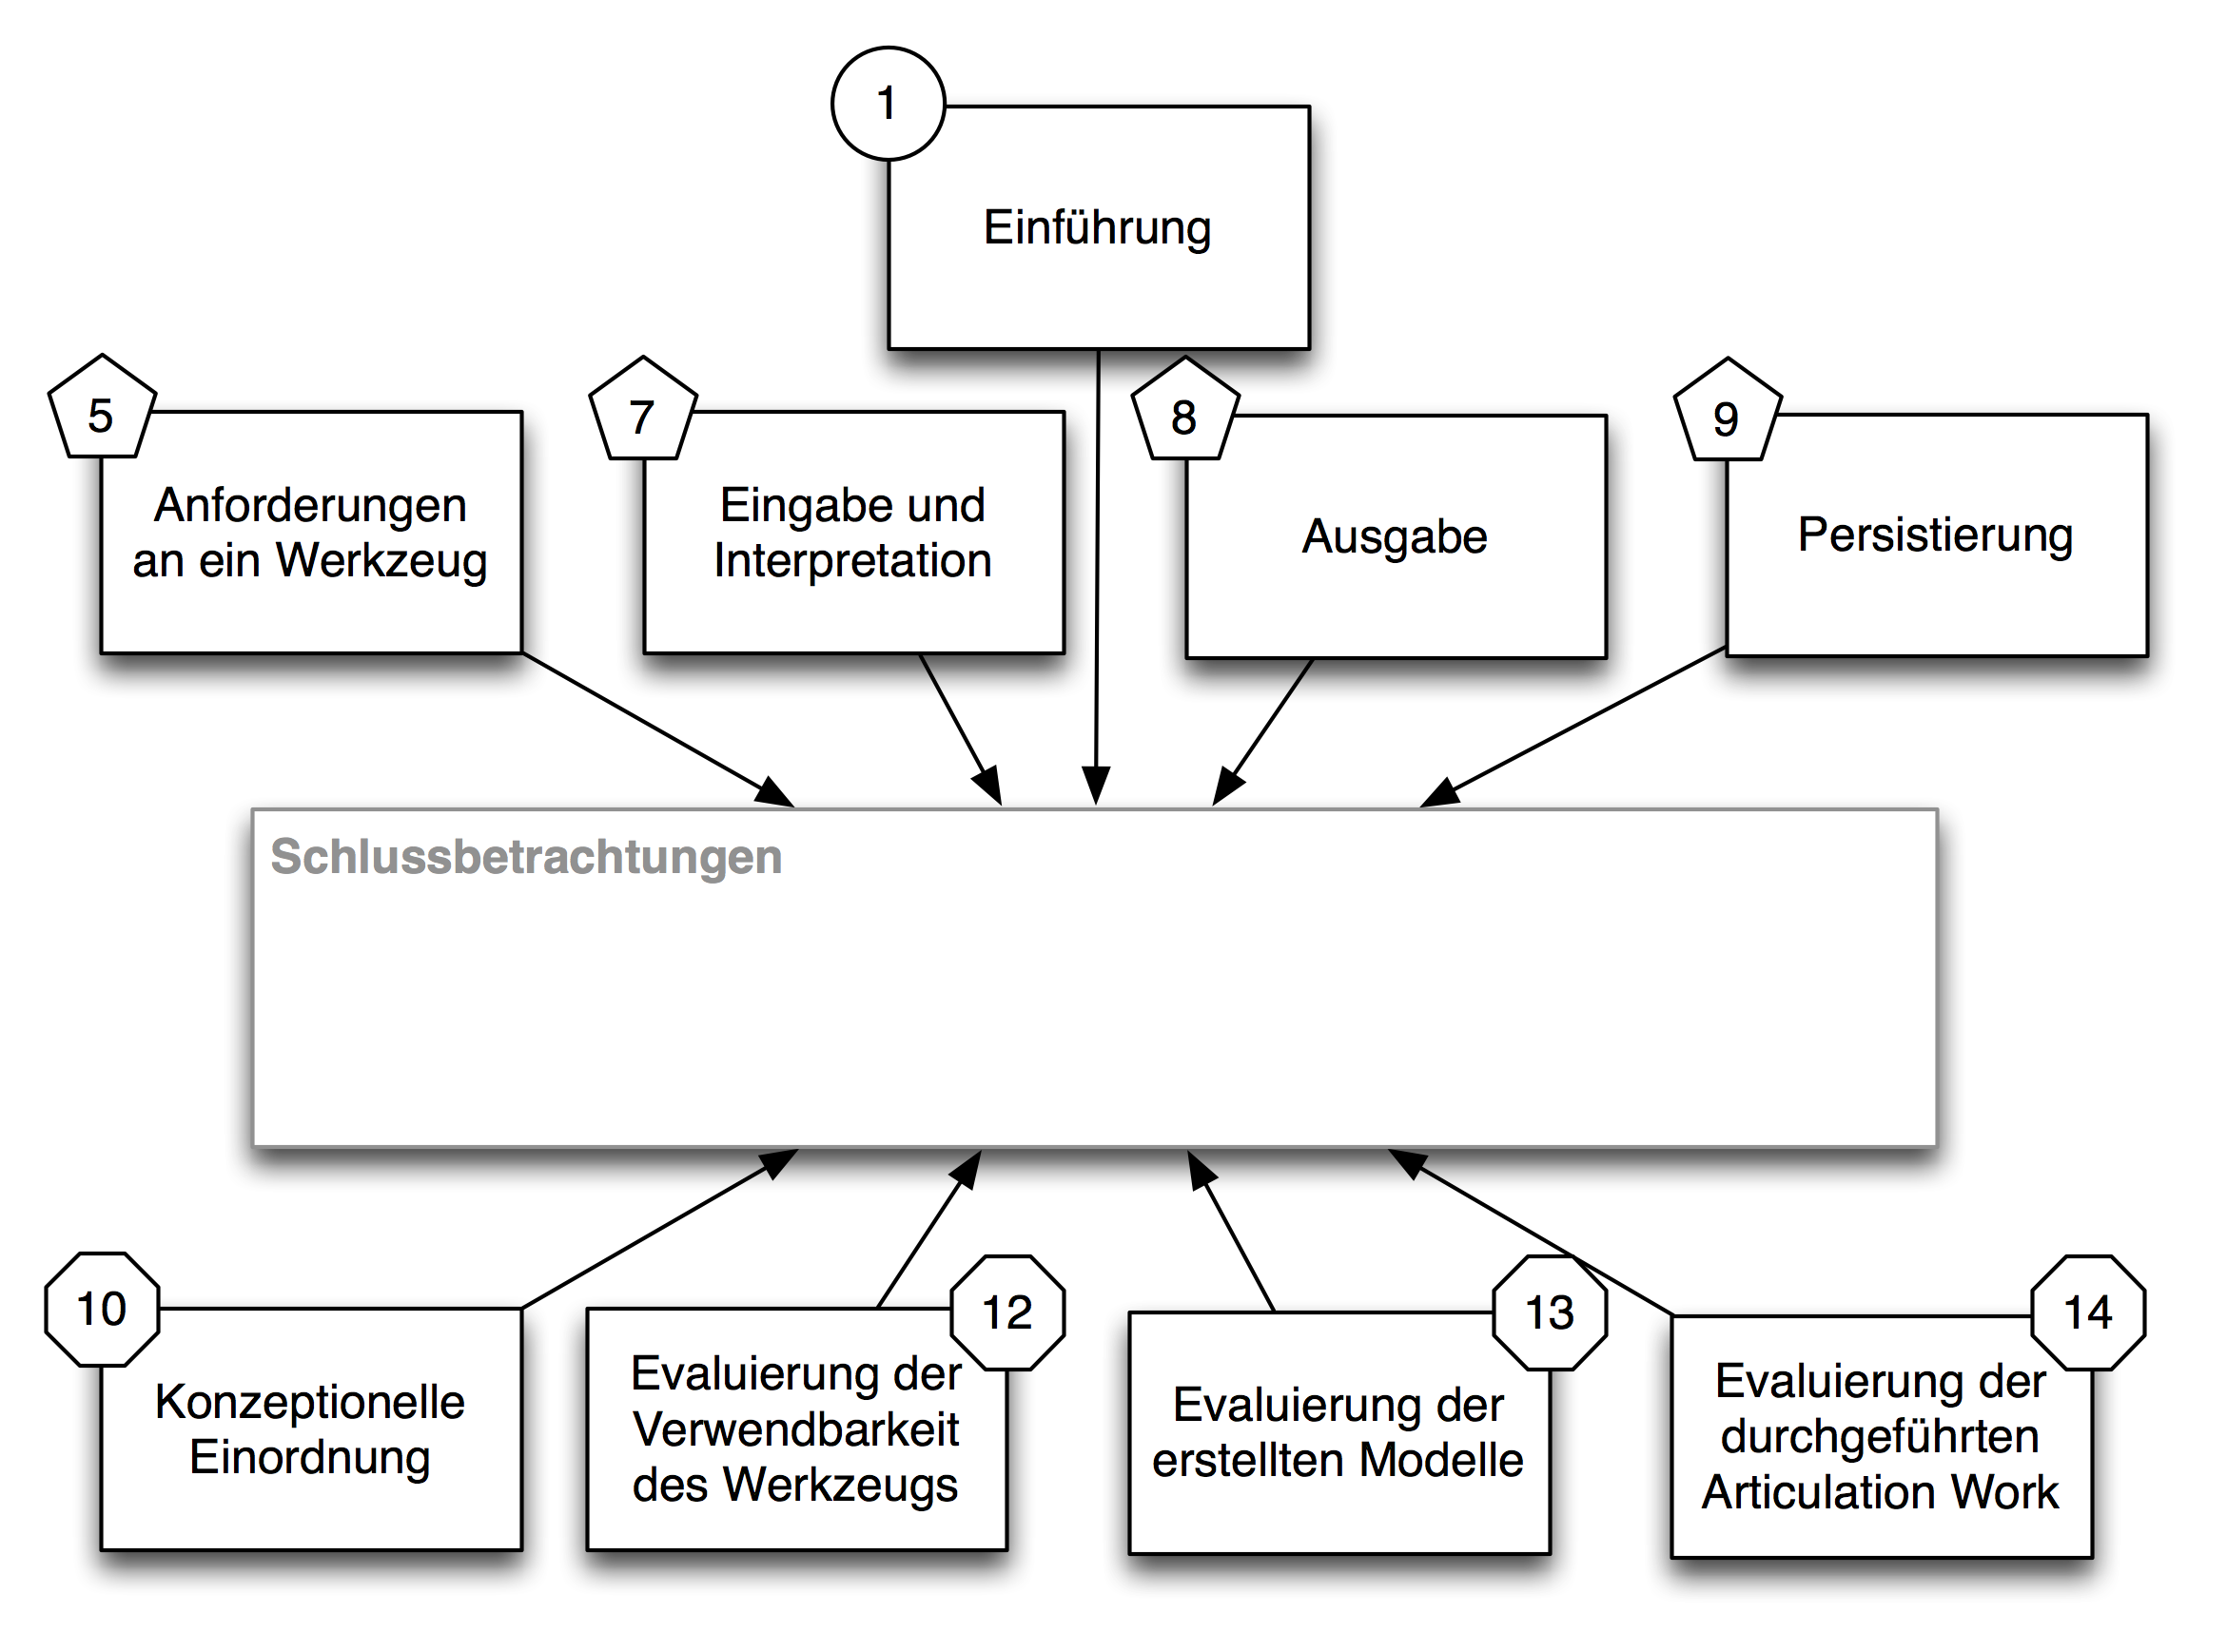
\includegraphics[scale=0.6]{img/Kontextgrafiken/k15.png}
	\caption{Kapitel „Schussbetrachtungen“ im Gesamtzusammenhang}
	\label{fig:img_Kontextgrafiken_k15}
\end{figure}

Abbildung \ref{fig:img_Kontextgrafiken_k15} zeigt die Kapitel, deren Ergebnisse in dieses Kapitel einfließen. Die einzelnen Inhalte werden schrittweise einander strukturiert gegenüber gestellt, was eine Beurteilung der Zielerreichung auf jeder Betrachtungsebene der Arbeit (Fragestellungen der empiririschen Untersuchung, Anforderungen an das Werkzeug, Globale Zielsetzung) ermöglicht. Nach einer Darstellung der gesamten dieser Arbeit zugrundeliegenden Konzepte und deren Zusammenhang in der Arbeit in Abschnitt \ref{sec:überblick_über_den_gesamtzusammenhang} werden die einzelnen oben genannten Betrachtungsebenen in umgekehrter Reihenfolge als in der Arbeit dargestellt (also vom Konkreten zum Allgemeinen) einzeln beschrieben. Nach einer Zusammenfassung der Evaluierungsergebnisse und einer Gegenüberstellung mit den Ergebnissen der konzeptuellen Einordnung in Abschnitt \ref{sec:zusammenfassung_der_evaluierung} werden diese in Abschnitt \ref{sec:erfüllung_der_anforderungen_an_das_werkzeug} den in Kapitel \ref{cha:anforderungen} angeführten Anforderungen an das Werkzeug gegenübergestellt. Im letzten Schritt werden die erreichten Ergebnisse hinsichtlich der globalen Zielsetzung bewertet (siehe Abschnitt \ref{sec:bewertung_hinsichtlich_der_globalen_zielsetzung}). Auf Basis dieser Ausführungen ist es in Abschnitt \ref{sec:offene_aspekte_und_entwicklungspotential} möglich, die noch offenen Aspekte dieser Arbeit und weiteres Entwicklungspotential zu identifizieren.

\section{Überblick über die Argumentation in dieser Arbeit} % (fold)
\label{sec:überblick_über_den_gesamtzusammenhang}

In Kapitel \ref{cha:einführung} wurde in Abbildung \ref{fig:img_ArticulationWork_ArbeitInteraktion} die dieser Arbeit zugrunde liegende Konzeptualisierung von Arbeit in „Production Work“ und „Articulation Work“ dargestellt. Auf Basis der Ausführungen in den dazwischen liegenden Kapiteln kann diese Abbildung wie in Abbildung \ref{fig:img_Schlussbetrachtungen_ArbeitInteraktionMentaleModelleTabletop} dargestellt erweitert werden und stellt so die gesamten konzeptionellen Grundbegriffe im Zusammenhang dieser Arbeit dar. Eine detailliertere Betrachtung der Ergebnisse unter Einbeziehung der tatsächlich umgesetzten technischen Unterstützung und den Ergebnissen der empirischen Evaluierung wird in Abschnitt \ref{sec:bewertung_hinsichtlich_der_globalen_zielsetzung} durchgeführt.

\begin{figure}[htbp]
	\centering
	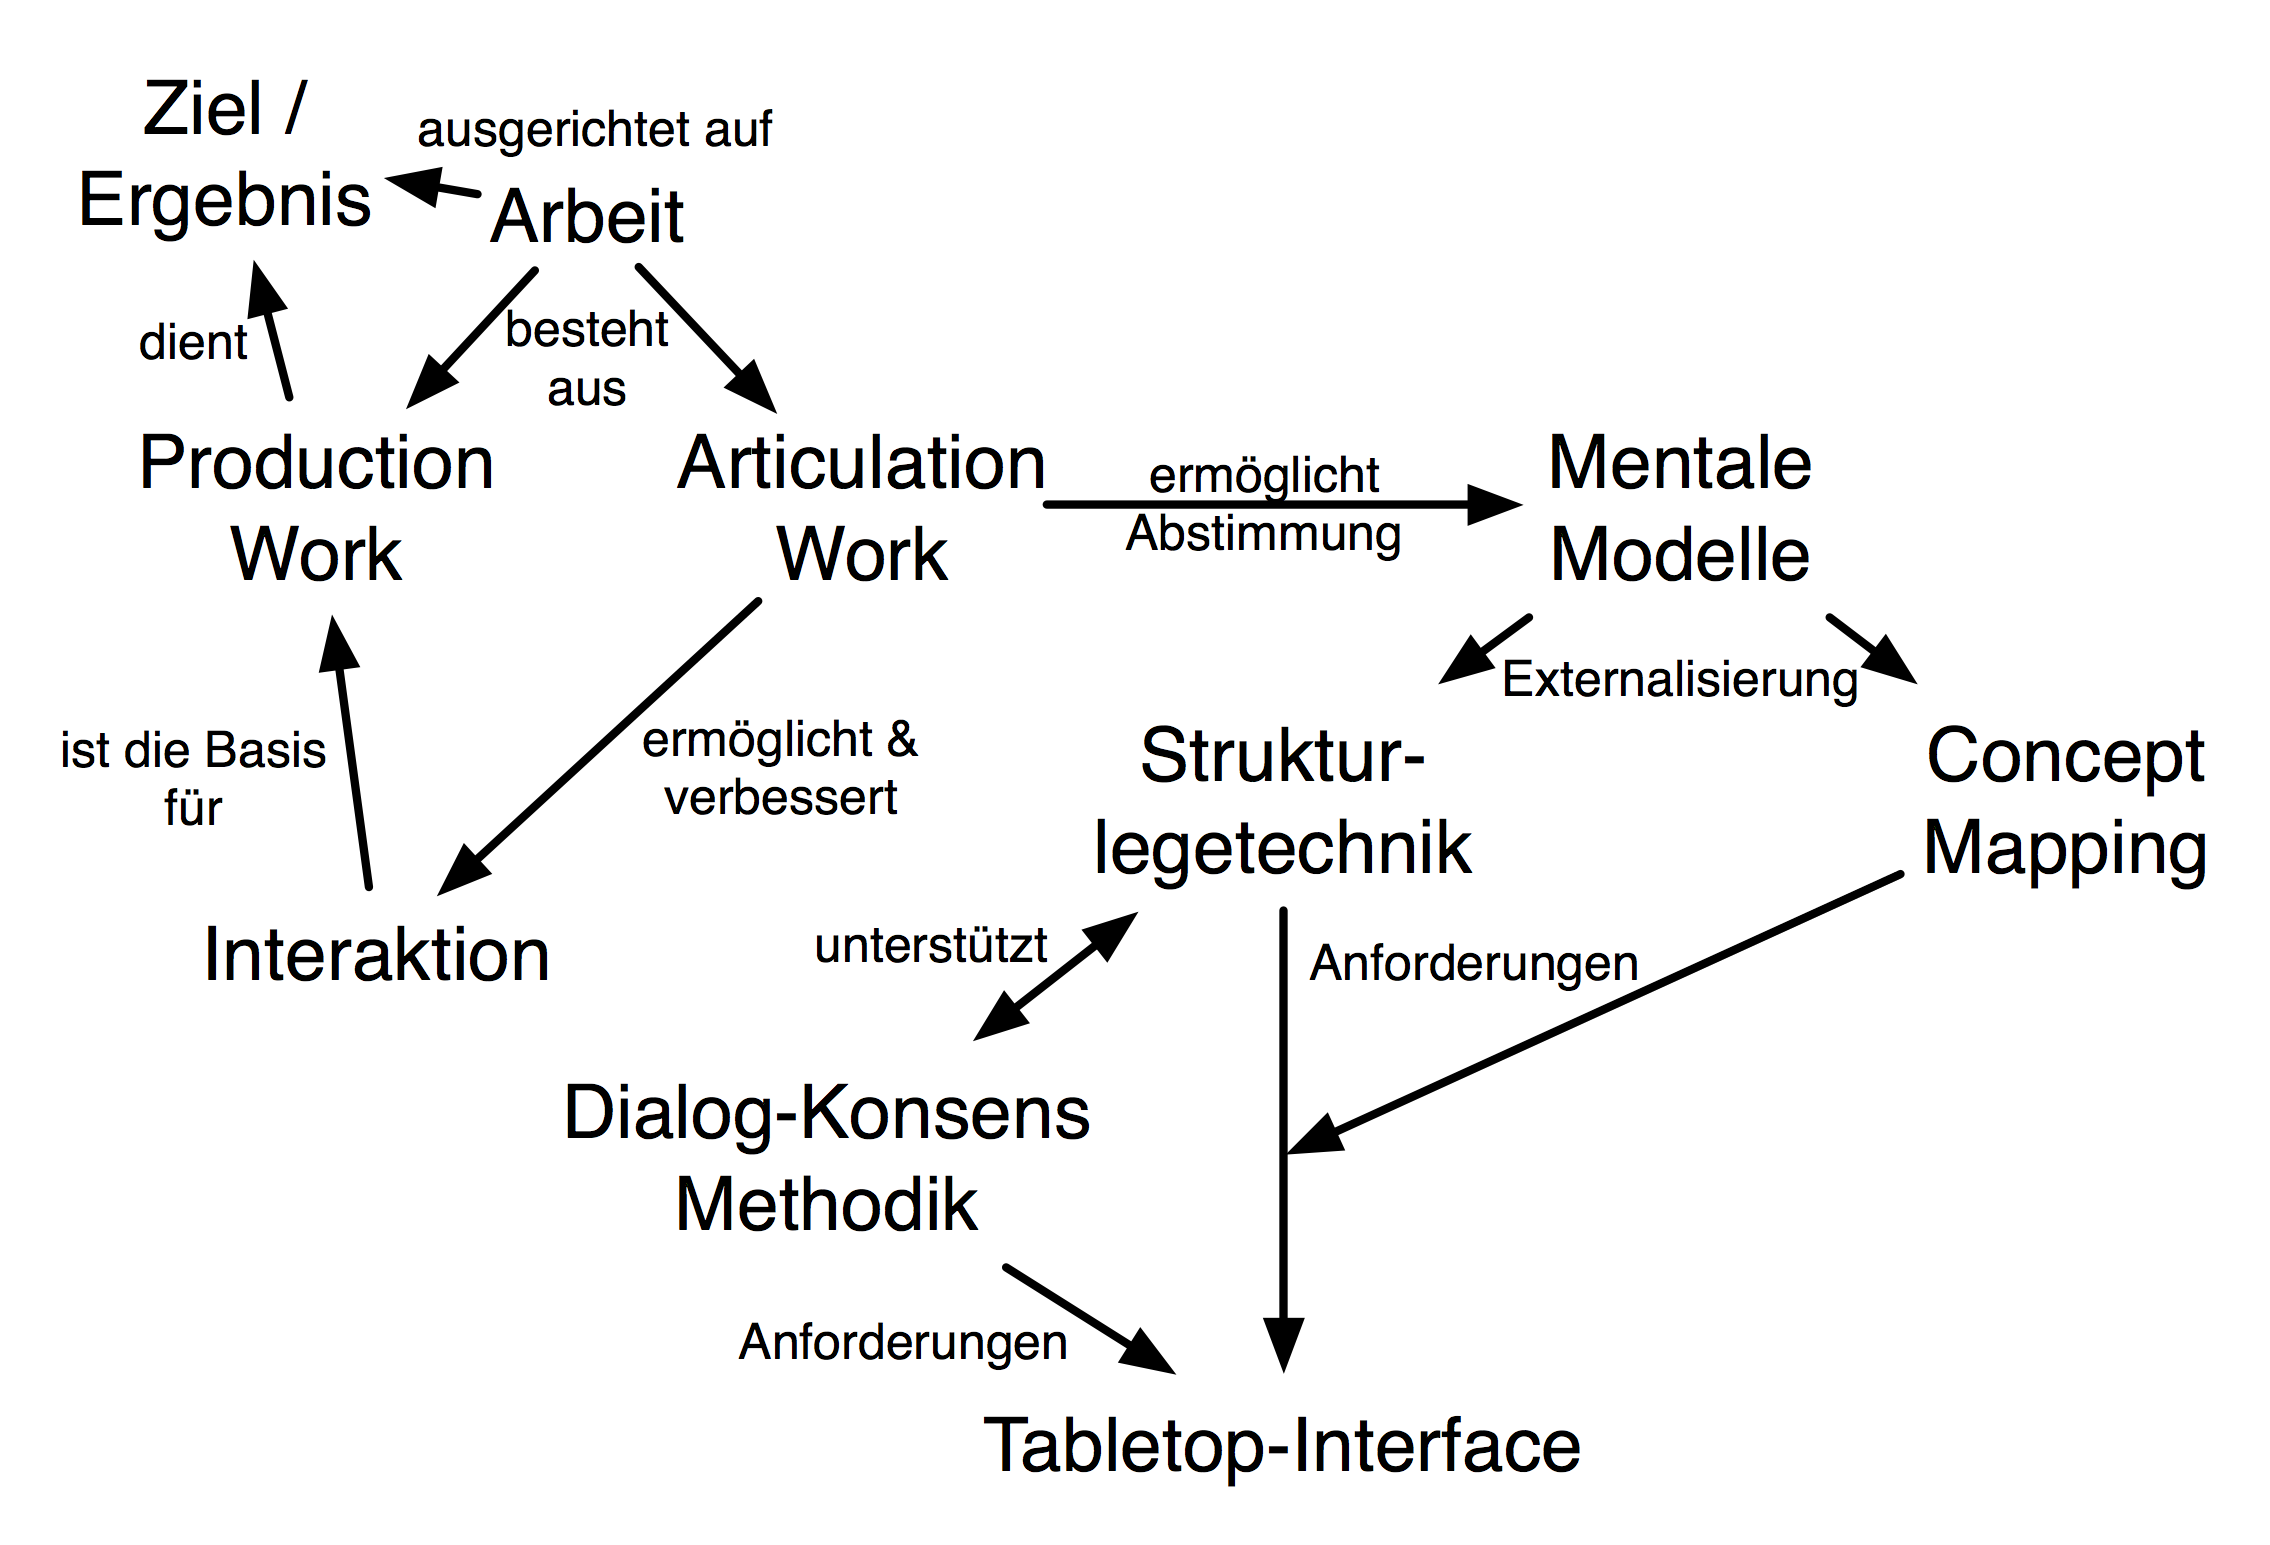
\includegraphics[width=0.9\textwidth]{img/Schlussbetrachtungen/ArbeitInteraktionMentaleModelleTabletop.png}
	\caption{Gesamtzusammenhang der verwendeten Konzepte}
	\label{fig:img_Schlussbetrachtungen_ArbeitInteraktionMentaleModelleTabletop}
\end{figure}

Das Ziel dieser Arbeit ist die Unterstützung der Auflösung von Situationen, in denen produktive Arbeit nicht (mehr) möglich ist. Dies ist dann der Fall, wenn unklar ist, wie die Zielerreichung gewährleistet werden kann. Diese Arbeit basiert auf der Annahme, dass Interaktion zwischen Individuen immer ein wesentlicher Aspekt bei der Durchführung von Arbeit ist. Arbeit enthält deshalb auch immer einen Anteil, der mit der Herstellung und Aufrechterhaltung der Interaktion der beteiligten bzw. betroffenen Individuen beschäftigt ist. Dieser Arbeitsanteil wird als „Articulation Work“ bezeichnet. Jedes beteiligte Individuum entwickelt auf Basis früherer Erfahrungen oder Lernprozessen Erklärungsmodelle (oder „Mentale Modelle“) für adäquate Aktivitäten bzw. Reaktionen im betreffenden Arbeitsablauf. Wesentlich für die erfolgreiche Interaktion mehrerer Individuen in einem Arbeitsablauf ist die Abstimmung dieser Erklärungsmodelle und die Entwicklung einer gemeinsamen Sichtweise auf jenen Teil des Arbeitsablaufs, in dem zusammengearbeitet werden muss. Diese Abstimmungsprozesse laufen implizit immer ab, wenn Individuen interagieren. In bestimmten, als komplex oder problematisch wahrgenommenen Arbeitssituationen reicht die implizite Abstimmung nicht mehr aus -- es ist notwendig, „Articulation Work“ explizit anzustoßen und den Abstimmungsvorgang bewusst zu unterstützen. Ein wesentlicher Schritt zur Abstimmung mentaler Modelle ist deren Externalisierung, also deren Abbildung in einer kommunizierbaren Form. Dazu werden unterschiedliche Methoden vorgeschlagen, denen gemein ist, dass die Abbildung in Form diagrammatischer Modelle erfolgt. In der konkreten Umsetzung unterscheiden sich die beiden Methoden „Strukturlegetechnik“ und „Concept Mapping“ voneinander, bieten aber beide Vorteile bei der Unterstützung der für „Articulation Work“ wichtigen Kommunizierbarkeit mentaler Modelle. In dieser Arbeit werden deshalb beide Ansätze berücksichtigt und in einer Methodik zusammengeführt, die an die im Rahmen von Strukturlegetechniken vorgeschlagene „Dialog-Konsens Methodik“ angelehnt ist. Generell hat bei der Konzeption der Werkzeugunterstützung der bei Strukturlegetechniken vorgeschlagene Ansatz das Primat, weil in ihm die kooperative Durchführung der Modellbildung explizit vorgesehen ist, was der Abstimmung mentaler Modelle eher entgegenkommt als der grundsätzlich eher individuell orientierte Concept-Mapping-Ansatz. Letztendlich wird also in dieser Arbeit der durch Strukturlegetechniken vorgeschlagene Ansatz des physischen, kooperativen Abbildung von Modellen verfolgt, weshalb die Abbildung der Modelle im physischen Raum, konkret auf eine kooperativ bearbeitbaren Tischoberfläche erfolgt. Die Berücksichtigung der Anforderungen des Concept Mapping begründet letztendlich die Notwendigkeit der Hinterlegung der physischen Modellierungsmöglichkeit mit computergestützten Werkzeugen. Um den Anspruch der physischen, kooperativen Modellbildung mit den computergestützten Unterstützungswerkzeugen zu vereinen, wird zur technologischen Umsetzung des Werkzeugs ein „Tabletop Interface“ verwendet, in dem beide Aspekte berücksichtigt und verknüpft werden können.

% section überblick_über_den_gesamtzusammenhang (end)

\section{Zusammenfassung der Evaluierung}
\label{sec:zusammenfassung_der_evaluierung}

In diesem Abschnitt wird die in den Kapiteln \ref{cha:eval_ueberblick}, \ref{cha:eval_werkzeug}, \ref{cha:eval_modell} und \ref{cha:eval_aw} beschriebene empirische Untersuchung zusammengefasst und den Ergebnissen der konzeptuellen Einordnung in Kapitel \ref{cha:konzeptionelle_evaluierung} gegenübergestellt.

\subsection{Empirische Untersuchung}

In der empirischen Untersuchung waren folgende in Kapitel \ref{cha:eval_ueberblick} formulierte Untersuchungsfragen zu beantworten:

\begin{itemize}
 \item Sind das Werkzeug und dessen Komponenten verständlich und wie intendiert einsetzbar? (Aspekt: Werkzeug)
 \item Erlauben Werkzeug und Methode die Abbildung semantisch offener diagrammatischer Modelle? (Aspekt: Modell)
 \item Unterstützen Werkzeug und Methode Articulation Work? (Aspekt: Articulation Work)
\end{itemize}

Jede dieser Fragen wurde in einem separaten Kapitel bearbeitet. Die Untersuchungsfragen wurden in Hypothese konkretisiert, die den jeweiligen Untersuchungsgegenstand in Bezug zu den aus den konzeptuellen Grundlagen abgeleiteten Anforderungen an die Unterstützung von Articulation Work stellen.

Bei der Betrachtung der ersten Untersuchungsfrage wurden 8 Hypothesen geprüft, die die grundlegenden Anforderungen an das Werkzeug abdecken bzw. die Verständlichkeit und Verwendbarkeit der implementierten Funktionen testen. Insgesamt scheint das Werkzeug für den intendierten Verwendungszweck -- der kooperativen Erstellung von diagrammatischen Modellen -- in unterschiedlichen Anwendungsgebieten einsetzbar zu sein. Stabilitätsprobleme in der technischen Umsetzung führten jedoch in den ersten Phasen der Evaluierung zu Behinderungen bei der Modellbildung, was jedoch durch nachträglich durchgeführte Verbesserungen weitgehend kompensiert werden konnte. Herausforderungen zeigten sich im Interaktionsdesign der über die Kernfunktionalität hinausgehenden Funktionen zur Unterstützung des Modellbildungsprozesses. Die aus der Literatur begründbare Funktion zur Verfolgung der Modellierungshistorie und der Wiederherstellung vergangener Modellzustände wurde kaum genutzt. Auch die Verwendung der Funktion zur Entfernung von unerwünschten Verbindern im Modell war den Benutzern in der ersten Version unverständlich. Dieses Problem konnte durch ein Redesign des entsprechenden Teilwerkzeugs und dessen Bedienung beseitigt werden. Generell scheint das Werkzeug schnell erlernbar zu sein, so dass die Anzahl der Fehlbedienungen durch Missverständnisse bereits bei der zweiten Anwendung des Werkzeugs durch die Benutzer massiv reduziert bzw. nicht mehr vorhanden war. Die oben formulierte Frage kann also mit Vorbehalten positiv beantwortet werden. Generell scheint das Werkzeug wie intendiert einsetzbar und zum Großteil verständlich zu sein, einige Komponenten weisen jedoch Defizite in der Verständlichkeit auf.

Für die zweite Untersuchungsfrage wurden 5 Hypothesen geprüft, die sich auf die Verwendung der Werkzeugs zur Modellbildung im Sinne der vorgeschlagenen Methodik zur Unterstützung von „Articulation Work“ beziehen. Insgesamt scheint das Werkzeug zwar nur eingeschränkt für die allgemeine Abbildung von Modellen beliebigen Inhalts und beliebiger Semantik geeignet zu sein, seinen Verwendungszweck für die auf Modellen basierende Kommunikation und Abstimmung von individuellen Sichtweise scheint das Werkzeug aber geeignet zu sein. Die eingeschränkte Eignung für die Abbildung beliebiger Modelle scheint vor allem in der beschränkten Größe der Modellierungsoberfläche begründet zu liegen, für die die Möglichkeit zur Einbettung von Teilmodellen keinen adäquaten Ersatz darzustellen scheint. Zudem scheint in Einzelfällen die in der aktuellen Hardware-Implementierung vorhandene Beschränkung auf drei semantisch unterschiedliche Modellelementtypen einschränkend wahrgenommen zu werden, was ebenfalls dem Anspruch eines semantisch vollständig offen Modellierungswerkzeugs widerspricht. Dies ist insofern zu relativieren, als dass die Anzahl der Elementtypen in den meisten Fällen zur Kommunikation der individuellen Sichtweisen auszureichen scheint und lediglich in Fällen zu gering wahrgenommen wird, wo eine „vollständige“ Abbildung eines Sachverhaltes angestrebt wurde. Generell scheint das Werkzeug deshalb bei der Modellierung für den intendierten Verwendungszweck in einem Großteil der Anwendungsfälle geeignet zu sein.

In der dritten Untersuchungsfrage wurde letztendlich geprüft, ob das Werkzeug im Sinne der globalen Zielsetzung tatsächlich „Articulation Work“ unterstützt. Dazu wurden 2 Hypothesen gebildet, die die zu erwartenden Wirkungen erfolgreicher „Articulation Work“ abdecken. Die unmittelbare Wirkung der Durchführung von „Articulation Work“ ist die Bildung eines gemeinsamen Verständnisses über den betrachteten Arbeitsgegenstand. Diese Wirkung konnte in der Untersuchung nachgewiesen werden, das Werkzeug erfüllt also diesen Teil der Anforderungen. Mittelbar sollte die Durchführung von „Articulation Work“ auch Auswirkungen auf die betrachteten Arbeitsabläufe selbst haben und die Interaktion im Idealfall verbessern. Derartige Wirkungen konnten jedoch in der Untersuchung nicht nachgewiesen werden. Einige Beobachtungen in Einzelfällen weisen auf eine entsprechende Wirkung hin, insgesamt kann diese aber nicht generalisiert werden. Ob dies am Werkzeug selbst festzumachen ist oder die in der Untersuchung betrachteten Arbeitsabläufe nicht optimal gewählt wurden, wird in weiteren Untersuchung zu prüfen sein.

\subsection{Gegenüberstellung der empirischen und konzeptuellen Untersuchung}
\label{sub:gegenüberstellung}

In diesem Abschnitt werden die Ergebnisse der empirischen Untersuchung den in in Abschnitt \ref{sub:verbesserungspotential_für_das_werkzeug} angeführten Konsequenzen für die Werkzeuggestaltung aus dessen konzeptueller Untersuchung gegenübergestellt.

In Kapitel \ref{cha:konzeptionelle_evaluierung} wurde das Werkzeug im Vorfeld der praktischen Untersuchung in die in Abschnitt \ref{sec:konzeptualisierungen_von_tangible_interfaces} beschriebenen Frameworks zur Beschreibung von Tangible Interfaces eingeordnet. Daraus konnte in Einzelaspekten Verbesserungpotetial für das Werkzeug abgeleitet werden, falls die tatsächliche Umsetzung einer Funktionalität des Werkzeugs nicht mit den konzeptionell begründbaren Designentscheidung übereinstimmte. In diesem Abschnitt wird nun angeführt, in welchen Fällen das Verbesserungpotential, d.h. im Umkehrschluss eine Schwäche der aktuellen Implementierung, in der empirischen Untersuchung bestätigt werden konnte. Die Ergebnisse erlauben eine qualitative Aussage über die Eignung der betrachteten Frameworks für die Konzeption von Tangible Interfaces.

\subsubsection{Missverständlichkeit des Löschtokens}

Die ursprüngliche Konzeption des Löschtokens zeigte eine Diskrepanz zwischen dessen wahrgenommener Verwendung und dem tatsächlichen Vorgehen bei dessen Einsatz. Diese Schwäche konnte aus mehreren Frameworks abgeleitet werden, da bei konsistenter Anwendung derselben das Interaktionsdesign anders als tatsächlich umgesetzt hätte ausfallen müssen.

Tatsächlich konnte die Mißverständlichkeit der Löschtokens in der empirischen Untersuchung bestätigt werden (siehe Abschnitt \ref{sub:verwendung_des_löschtokens}). Nach einem Redesign der Verwendung des Löschtokens unter Berücksichtigung der konzeptuell indizierten Gestaltungs-Kriterien traten keine Mißverständnisse mehr auf, das Ausmaß des Einsatzes stieg signifikant an.


\subsubsection{Schwache Ein-Ausgabe-Kopplung bei der Modellierungshistorie}

Nach der Aktivierung der Modellierungshistorie wird diese ausschließlich durch ein Werkzeug auf der Modellierungsoberfläche kontrolliert. Die Ausgabe erfolgt jedoch ausschließlich auf dem sekundären Ausgabekanal, auf der Tischoberfläche erfolgt kein visuelles Feedback weder über die Aktivierung des Historienmodus noch über deren aktuellen Zustand (konkret die aktuelle Position in der Zeitlinie). Nach \citep{Ullmer00} wäre diese schwache Kopplung zu hinterfragen.

In der empirischen Untersuchung konnte dieser Aspekt nicht als Schwachstelle bestätigt werden. Die Entkopplung von Kontrolle und Ausgabe in diesem Anwendungsfall wurde von keinem Teilnehmer als missverständlich wahrgenommen und führte auch nie zu Fehlbedienungen. Dies mag daran liegen, dass der sekundäre Ausgabekanal räumlich nahe an der Tischoberfläche angeordnet war und von vielen Teilnehmern bei der Modellerstellung ohnehin als primäre Informationsquelle -- noch vor der Tischoberfläche selbst -- genutzt wurde. Erst bei der Diskussion verlagerte sich der Fokus der Aufmerksamkeit hin zu dem auf der Tischoberfläche gelegten Modell. Die von der herkömlichen Interaktionsform mit Maus und Tastatur vertraute entkoppelte Ein- und Ausgabe scheint in diesem Fall Bedienungsprobleme vermieden zu haben. Dass keine Desorientierung der Benutzer beim Wechsel in den Historienmodus auftrat, scheint damit zu begründen sein, dass der sekundäre Ausgabekanal permanent aktiv war, den Modellzustand immer synchron darstellte und deshalb wie oben erwähnt oft ohnehin als primärer Informationskanal genutzt wurde.  

\subsubsection{Lange Antwortzeiten auf Interaktionen}

In der ersten Implementierung des Systems kam es vor allem bei der Interaktion zur Herstellung von Verbindern zu Verzögerungen in der Reaktion des Systems. Diese Verzögerungen sollten nach \citep{Bellotti02} vermieden werden, um den Benutzern adäquat Rückmeldung über deren Interaktionswunsch geben zu können.

In der empirischen Untersuchung konnte diese Schwachstelle bestätigt werden. Die Möglichkeit zur Herstellung von Verbindern wurde in der ursprünglichen Implementierung kaum genutzt. Erst als eine weitere Möglichkeit zur Herstellung von Verbindern implementiert wurde, deren wahrgenommer Reaktionszeit geringer war, wurde diese Möglichkeit in signifikant höherem Ausmaß genutzt (siehe Abschnitt \ref{sub:herstellung_von_verbindern}).

\subsubsection{Fehlende einfache Undo-Funktion}

Die Möglichkeit zur Wiederherstellung von vergangenen Modellzuständen ("Undo") ist in der aktuellen Implementierung zwar gegeben, bedingt aber eine zeitaufwändige und in mehreren Schritten durchzuführende Interaktion mit dem System. Dies sollte nach \citep{Bellotti02} vermieden werden, auch das Schema von \citep{Shaer04} lässt hier Inkonsistenzen mit den den ansonsten ausschließlich einschrittigen Interaktionen mit dem Werkzeug erkennen.

In der empirischen Untersuchung wurde die Möglichkeit zur Wiederherstellung zwar verwendet, das Ausmaß des Einsatzes sank aber signifikant, als das Löschtoken neu gestaltet wurde und so eine einschrittige Interaktion zur Korrektur von fehlerhaften Verbindungen (dem häufigsten Grund des Einsatz der Undo-Funktion) geschaffen wurde. Die Gestaltung der Wiederherstellungsfunktion kann damit als Schwachstelle bestätigt werden.

\subsubsection{Mangelnde Verständlichkeit des Snapshot-Tokens}

Das Design des Snapshot-Tokens weist in der derzeitigen Umsetzung nicht auf dessen Funktion hin, was nach bei einer Einordnung in die Taxonomie nach \citep{Fishkin04} gegenüber den anderen Werkzeugen inkonsistent ist. Das Token suggeriert zwar nicht wie im Fall des Löschtoken eine andere Funktionalität, gibt aber den Benutzern durch sein Erscheinungsbild keinen Hinweis auf die Verwendung (mangelhafte Affordances \citet{Norman90}).

Tatsächlich zeigt sich in der empirischen Untersuchung, dass die Funktion zur expliziten Erfassung von Snapshots kaum bzw. in den meisten Anwendungen nicht verwendet wird. Trotz einer erklärenden Einführung in das Werkzeug vor der Modellbildung bestehen häufig Unklarheiten zur Verwendung des Tokens, sobald Benutzer während der Anwendung damit konfrontiert werden. Auch diese Designentscheidung ist damit als Schwachstelle zu bestätigen. 

\subsubsection{Funktional belegte Bereich der Modellierungsoberfläche}

Der hier beschriebene Aspekt ist keine Schwachstelle des Werkzeugs sondern eine Erweiterungsmöglichkeit, die auf Basis der Ausführungen von \citep{Ishii97} identifiziert wurde. Die Autoren schlagen vor, Teile der Interaktionsoberfläche („Trays“) mit Funktionen zu belegen, die eine bestimmte Operation auf einem auf ihm platzierten Token ausführen (etwa: „Details anzeigen“). Bei der Umsetzung des Werkzeugs wurde diese Möglichkeit nicht berücksichtigt, es sind jedoch sinnvolle Anwendungsmöglichkeiten denkbar.

In der empirischen Untersuchung wurden derartige Funktionen von keinen Benutzern erwartet oder gefordert. Da diese Form der Interaktion aber nicht der gängigen Desktop-Metapher entspricht, ist dies auch nur eingeschränkt zu erwarten. Es kann damit auf Basis der Untersuchung keine Aussage über die Notwendigkeit oder Sinnhaftigkeit einer derartigen Erweiterung getroffen werden.

\subsubsection{Verwendbarkeit frei wählbarer Tokens}

Zur Anpassung des Modellierungswerkzeugs an die jeweilige Anwendungsdomäne führt \citep{Holmquist99} als Möglichkeit die Verwendung von domänenspezifischen Token an. Diese Forderung ist grundsätzlich mit den Ansprüchen der semantischen Offenheit des Werkzeugs und der domänenübergreifenden Anwendbarkeit des Ansatzes vereinbar und stützt diese. In der derzeitigen Implementierung ist die Zahl der unterschiedlichen Modellelementtypen auf drei begrenzt. Diese Elementtypen sind in generischen Formen ausgeführt und per se nicht intuitiv domänenspezifisch interpretierbar.

In der empirischen Untersuchung wurde mehrfach die Forderung nach einer höheren Anzahl von unterschiedlichen Elementtypen geäußert, was aber die hier betrachtete Erweiterungsmöglichkeit nur am Rande betrifft (die Verwendung beliebiger Elementtypen würde deren Anzahl zwar erhöhen, umgekehrt implizit die Forderung nach mehr Elementtypen nicht jene nach beliebigen Ausprägungen derselben). Tatsächlich wurde aber in einigen Anwendungen explizit der Wunsch geäußert, Objekt aus dem spezifischen Anwendungsfall (etwa Dokumente oder Werkzeuge) als Tokens verwenden zu können. Dies entspricht im Wesentlichen der oben beschriebenen Erweiterungsmöglichkeit, weshalb die Erweiterungsmöglichkeit als sinnvoll erachtet werden kann. 

\section{Erfüllung der Anforderungen an das Werkzeug}
\label{sec:erfüllung_der_anforderungen_an_das_werkzeug}

In diesem Abschnitt werden die in Kapitel \ref{cha:anforderungen} formulierten Anforderungen an das Werkzeug hinsichtlich ihrer Erfüllung betrachtet. Die Beurteilung der Erfüllung erfolgt anhand der empirischen Ergebnisse, die in den Kapiteln \ref{cha:eval_werkzeug}, \ref{cha:eval_modell} und \ref{cha:eval_aw} beschrieben wurden.

Anforderung \ref{anf:physische_abbildung_legen_beliebiger_diagrammatischer_modelle} (Physische Abbildung beliebiger diagrammatischer Modelle) wurde in den Hypothesen \ref{hyp:diagmodelle}, \ref{hyp:behinderung} und \ref{hyp:gewöhnung} untersucht. Die grundlegende Abbildung diagrammatischer Modelle mit dem Werkzeug ist ohne Einschränkung der Anwendungsdomäne möglich. Bei der Untersuchung des Prozesses der physischen Abbildung der Modelle konnten in den ersten durchgeführten Evaluierungsblöcken behindernde Aspekte identifiziert werden. Diese hatten Einfluss auf die Abbildung der Modelle, insbesondere die Möglichkeit des Einsatzes von Verbindern im Modell wurde nur eingeschränkt wahrgenommen. Nach Überarbeitungen des Interaktionsdesigns und der Implementierung mehrerer Maßnahmen zur Steigerung der Robustheit gegenüber Fehlerkennungen von Benutzereingaben konnten die als behindernd wahrgenommenen Faktoren reduziert werden. Bei mehrmaliger Verwendung des Werkzeugs zeigt sich eine Verbesserung des Umgangs mit den zur Verfügung gestellten Ausdrucksmöglichkeiten und eine stärke Fokussierung auf den zu repräsentierenden Sachverhalt. Insgesamt kann diese Anforderung als erfüllt angesehen werden.

Anforderung \ref{anf:unterstützung_der_iterativen_aushandlung_des_modells} (Unterstützung der iterativen Aushandlung des Modells) wurde in der Hypothese \ref{hyp:abstimmung} untersucht. Ziel der Unterstützung von Aushandlungsprozessen ist die Bildung einer gemeinsamen Sichtweise auf das betrachtete Problem. Die kooperative Modellierung ist durch das Design von Hard- und Software grundsätzlich möglich, durch die Verwendung eines Tabletop Interface wird die kooperative Modellbildung und der Austausch über den Modellierungsgegenstand (also das betrachtete Problem) ermöglicht. Die beabsichtigte Wirkung der Abstimmung der individuellen Sichtweisen konnte in der empirischen Untersuchung bestätigt werden. Insgesamt kann diese Anforderung also bestätigt werden.

Anforderung \ref{anf:ermöglichung_experimenteller_veränderungen_am_modell} (Ermöglichung experimenteller Veränderungen am Modell) wurde in der Hypothese \ref{hyp:wiederherstellung} untersucht. Experimentelle Veränderungen am Modell werden durch die Unterstützung der Wiederherstellung von vergangenen Modellzuständen realisiert. Diese Funktion wurde technisch implementiert und hinsichtlich ihrer Funktionsfähigkeit getestet. Diese ist vollständig gegeben. In der empirischen Untersuchung wurde die Funktionalität von den Teilnehmern jedoch nicht genutzt, so dass die Erfüllung der Anforderung empirisch nicht bestätigt werden kann. Aus den Ergebnissen der Untersuchung ist vielmehr zu hinterfragen, ob diese aus der Theorie der Externalisierung mentaler Modelle abgeleitete Anforderung in der Praxis tatsächlich relevant ist.

Anforderung \ref{anf:nicht_vorgegebene_semantik_der_modellierungselemente} (Nicht vorgegebene Semantik der Modellierungselemente) wurde in den Hypothesen \ref{hyp:kontexte} und \ref{hyp:keine_einschränkung} untersucht. Durch die nicht vorgegebene Semantik der Modellierungselemente wird einerseits der Einsatz des Werkzeugs in unterschiedlichen Anwendungskontexten ermöglicht, andererseits werden Benutzer nicht gezwungen, ein vorgegebenes Abbildungsschema für die von ihnen auzudrückende Information zu verwenden. Dies ermöglicht ein Fokussierung auf die Modellierungsinhalte und die Kommunikation derselben und vermeidet einen zusätzlichen kognitiv belastenden Übersetzungsschritt. Technisch wurde diese Anforderung durch die Verwendung generischer (also semantisch nicht vorbelegter) Modellierungsbausteine in Kombination mit dem Einsatz von Topic Maps zur Repräsentation der Modelle umgesetzt. Das Werkzeug erlaubt grundsätzlich die Verwendung von beliebigen und beliebig vielen unterschiedlichen Modellierungsbausteinen, diese Möglichkeit wurde jedoch im vorliegenden Prototypen nicht eingesetzt. Die empirische Untersuchung konnte die Einsetzbarkeit in unterschiedlichen Anwendungskontexten ohne Einschränkung bestätigen. Die Modellierung selbst wurde jedoch durch die im Prototypen auf drei unterschiedliche Modellierungselemente eingeschränkte Ausdrucksstärke des Werkzeugs teilweise als einschränkend empfunden. Da dies jedoch keine konzeptionelle Einschränkung ist, sondern ausschließlich dem aktuellen Entwicklungsstand der Werkzeug-Hardware geschuldet ist, kann diese Anforderung insgesamt als erfüllt angesehen werden. 

Anforderung \ref{anf:verknüpfung_mit_digitalen_ressourcen} (Verknüpfung mit digitalen Ressourcen) wurde im Rahmen der empirischen Untersuchung nicht berücksichtigt. Die Verknüpfung mit digitalen Ressourcen wurde analog zur Funktion zur Einbettung von Teilmodellen implementiert. Digitale Dokumente können an einbettbare Tokens gebunden werden und in einem Container durch Hineinlegen zugewiesen werden. Diese Funktionalität wurde technisch implementiert und hinsichtlich ihrer Funktionsfähigkeit getestet. Im Rahmen der Evaluierung wurde das Werkzeug ausschließlich mit einem Rechner betrieben, auf dem keine fallspezifischen bzw. anwendungsrelevanten digitalen Dokumente vorhanden waren. Die Einbindung von Dokumenten in Modelle konnte deswegen nicht vorgenommen werden. Die Anforderung ist also technisch erfüllt, konnte jedoch empirisch nicht überprüft werden. 

Anforderung \ref{anf:bearbeitung_von_beliebig_komplexen_modellen} (Bearbeitung von beliebig umfangreicher Modellen) wurde in der Hypothese \ref{hyp:beliebige_komplexität} untersucht. Durch die phyisch beschränkte Größe der Modellierungsfläche konnte die Erweiterung der Modellgröße lediglich durch die Erstellung von Teilmodellen erreicht werden, wobei deren Zusammenhang durch die Einbettung der Teilmodelle in Überblicksmodelle ausgedrückt wird. Die Einbettbarkeit von Teilmodellen wurde mittels der Verwendung von Modellierungsblöcken als Container realisiert, in die Tokens als Repräsentaten der Teilmodelle gelegt werden können. Die dazu notwendigen Funktionen wurden technisch implementiert und hinsichtlich ihrer Funktionsfähigkeit erfolgreich getestet. Auch in der empirischen Untersuchen wurde die Erweiterung der Modellgröße durch Einbettung von Teilmodellen erfolgreich eingesetzt. Im Vergleich der erstellten Modelle mit Modellen, die mit einem Werkzeug mit nicht beschränkter Modellierungsfläche erstellt wurden, zeigte sich jedoch eine signifikant geringere Modellgröße bei der Erstellung mit dem hier vorgestellten System. Die Erstellung beliebig großer Modelle ist somit technisch grundsätzlich möglich und auch verwendbar, empirisch konnte die Erfüllung der Anforderung dennoch nicht nachgewiesen werden.

Anforderung \ref{anf:kollaborative_und_unmittelbare_manipulierbarkeit_des_modells} (Kooperative und unmittelbare Manipulierbarkeit des Modells) wurde in den Hypothesen \ref{hyp:kollaborativ} und \ref{hyp:stärkere_kooperation} untersucht. Die Möglichkeit, Modelle kooperativ zu erstellen und zu manipulieren, ist grundsätzlich gegeben, die Möglichkeit der Durchführung eines kooperativen Modellierungsprozesses konnte empirisch belegt werden. Im Vergleich zu einem bildschirmbasierten System zeigt sich außerdem ein signifikant höherer Anteil an Interaktion zwischen den Teilnehmern bei der Durchführung der Modellierung mit dem hier vorgestellten System. Die Anforderung kann somit als erfüllt angesehen werden.

Anforderung \ref{anf:persistente_ablage_des_modells_möglichkeit_zur_rekonstruktion} (Persistente Ablage des Modells und Möglichkeit zur Rekonstruktion) wurde in der Hypothese \ref{hyp:historie} untersucht. Die Persistente Ablage der erstellten Modelle wurde mittels XML-Topic Maps realisiert. Die Funktionsfähigkeit der Persistierung wurde insofern technisch nachgewiesen, als dass die exportierten Modellrepräsentationen valide \gls{XTM}-Dateien waren und sämtliche auf der Modellierungsoberfläche repräsentierte Information in der Datei abgebildet war. Hinsichtlich der Ermöglichung der Rekonstruktion und der Nachvollziehbarkeit des Modellierungsprozesses konnte gezeigt werden, dass die bei der Persistierung inkludierte Entstehungshistorie des Modells die Nachvollziehbarkeit der im Modell repräsentierten Information zwar tendenziell erleichterte, aber nicht in allen Fällen ermöglichte. Die Anforderung kann damit technisch als erfüllt angesehen werden, die positive Wirkung der eingebetteten Entstehungshistorie des Modells konnte ebenfalls bestätigt werden. Insgesamt ist die Nachvollziehbarkeit der Modelle ausschließlich auf Basis der gespeicherten Repräsentationen aber in Frage zu stellen.

Zusammenfassend ergibt sich hinsichtlich der Erfüllung der Anforderungen die in Tabelle \ref{tab:erfuellung_der_anforderungen} dargestellte Übersicht. In ihr sind die Anforderungen jenen Kapiteln und Abschnitten des Implementierungsteils (\emph{Impl.}) zugewiesen, in denen ihre technische Umsetzung beschrieben wird, sowie den Hypothesen (\emph{Hyp.}) zugeordnet, in denen die tatsächliche Überprüfung der Erfüllung durchgeführt wird.

\begin{table}[htbp]
	\centering
	\caption{Erfüllung der Anforderungen}
\begin{tabular}{| c | p{5cm} | p{1cm} | c | p{4cm} |} 
  \hline
  & Anforderung & Impl. & Hyp. & Beurteilung \\ \hline \hline
  \ref{anf:physische_abbildung_legen_beliebiger_diagrammatischer_modelle} & Physische Abbildung beliebiger diagrammatischer Modelle &  \ref{sub:erkennen_von_verbindungen}, \ref{sub:benennung_von_modellelementen}, \ref{sub:ausgabe_von_information_zum_modell} & \ref{hyp:diagmodelle}, \ref{hyp:behinderung}, \ref{hyp:gewöhnung} & technisch möglich, empirisch teilweise bestätigt \\ \hline
  \ref{anf:unterstützung_der_iterativen_aushandlung_des_modells} & Unterstützung der iterativen Aushandlung des Modells & \ref{ssub:zustands_und_ereignismeldungen} & \ref{hyp:abstimmung} & technisch möglich, empirisch bestätigt \\ \hline
  \ref{anf:ermöglichung_experimenteller_veränderungen_am_modell} & Ermöglichung experimenteller Veränderungen am Modell & \ref{sub:tracking_des_modellzustandes}, \ref{ssub:wiederherstellungsunterstützung} & \ref{hyp:wiederherstellung} & technisch möglich, empirisch nicht bestätigt \\ \hline \hline
  \ref{anf:nicht_vorgegebene_semantik_der_modellierungselemente} & Nicht vorgegebene Semantik der Modellierungselemente & \ref{sub:festlegung_der_bedeutung_von_modellelementen}, \ref{sub:abbildung_des_metamodells} & \ref{hyp:kontexte}, \ref{hyp:keine_einschränkung} & technisch möglich, empirisch teilweise bestätigt \\ \hline
  \ref{anf:verknüpfung_mit_digitalen_ressourcen} & Verknüpfung mit digitalen Ressourcen & \ref{sub:erkennung_von_geöffneten_tokens}, \ref{sub:ausgabe_von_information_zum_modell} & --- & technisch möglich, empirisch nicht geprüft \\ \hline
  \ref{anf:bearbeitung_von_beliebig_komplexen_modellen} & Bearbeitung von beliebig umfangreicher Modellen & \ref{sub:erkennung_von_geöffneten_tokens} & \ref{hyp:beliebige_komplexität} & technisch möglich, empirisch nicht bestätigt \\ \hline \hline
  \ref{anf:kollaborative_und_unmittelbare_manipulierbarkeit_des_modells} & Kooperative und unmittelbare Manipulierbarkeit des Modells & \ref{sub:verteilung_des_modellzustandes}, \ref{sub:einsatz_von_jhotdraw} & \ref{hyp:kollaborativ}, \ref{hyp:stärkere_kooperation} & technisch möglich, empirisch bestätigt \\ \hline
  \ref{anf:persistente_ablage_des_modells_möglichkeit_zur_rekonstruktion} & Persistente Ablage des Modells und Möglichkeit zur Rekonstruktion & \ref{sub:tracking_des_modellzustandes}, \ref{ssub:abruf_der_modellierungshistorie}, \ref{sub:grundlegende_abbildung} & \ref{hyp:historie} & technisch möglich, empirisch bestätigt \\ \hline 
\end{tabular}
	\label{tab:erfuellung_der_anforderungen}
\end{table}


\section{Bewertung hinsichtlich der globalen Zielsetzung}
\label{sec:bewertung_hinsichtlich_der_globalen_zielsetzung}

In diesem Abschnitt wird die Arbeit hinsichtlich der globalen Zielsetzung zusammengefasst, reflektiert und beurteilt. In Kapitel \ref{cha:einführung} wurde die globale Zielsetzung wie folgt formuliert:

\fbox{\parbox{13cm}{\textbf{In der vorliegenden Arbeit sind die methodischen und technischen Möglichkeiten zur Ermöglichung und Unterstützung von expliziter Articulation Work zu ergründen, die gewonnenen Erkenntnissen in einem Werkzeug umzusetzen und dessen Auswirkungen auf die Interaktion zur Verbesserung der Production Work zu bewerten.}}}

Zur Detaillierung dieser Zielsetzung wurden drei Forschungsfragen formuliert, die im Folgenden in die Betrachtung einfließen:
\begin{enumerate}
	\item Wie kann explizite Articulation Work ermöglicht und unterstützt werden?
	\item Was muss ein Werkzeug zur Unterstützung von expliziter Articulation Work leisten?
	\item Inwiefern unterstützt das entwickelte Werkzeug die Durchführung von Articulation Work?
\end{enumerate}

Bei der Reflexion der Ergebnisse dieser Arbeit hinsichtlich der Forschungsfragen wird jeweils auch auf den Kontext der Arbeit, aus dem die Ableitung der Zielsetzung heraus durchgeführt wurde, Bezug genommen.

\subsection{Wie kann explizite Articulation Work ermöglicht und unterstützt werden?}

Die globale Zielsetzung stellt den Anspruch, die methodischen und technologischen Möglichkeiten der Unterstützung expliziter „Articulation Work“ zu untersuchen. Die Festlegung bzw. Einschränkung auf explizite „Articulation Work“ dient der Abgrenzung der Arbeit zu Ansätzen, die sozial und/oder technologisch in Arbeitsabläufe intervenieren und dem Auftreten von Unklarheiten vorbeugen bzw. diese durch unmittelbare Unterstützungmaßnahmen auflösen. All diese Ansätze sind in den Bereich der impliziten „Articulation Work“ einzuordnen, die Durchführung derselben ist den handelnden Personen also nicht unbedingt bewusst. Treten Situationen auf, die von den Beteiligten als so problematisch wahrgenommen werden, dass eine Aufrechterhaltung des Arbeitsablaufs nicht mehr gewährleistet ist, muss die Handlungsfähigkeit durch explizite Beschäftigung mit der problematischen Situation (wieder) hergestellt werden. Dieser Fall wird als explizite „Articulation Work“ bezeichnet. Das Abbruchkriterium für explizite „Articulation Work“ ist das Erreichen eines Zustandes, in dem soweit gegenseitiges Verständnis hergestellt ist, dass die produktiven Arbeitsabläufe durch implizite „Articulation Work“ aufrecht erhalten werden können. Es müssen somit die methodischen und technischen Voraussetzungen zur erfolgreichen (Wieder-)Erlangung einer gemeinsamen Sichtweise aller Beteiligten auf den als problematisch wahrgenommenen Betrachtungsgegenstand geschaffen werden.

Ein Erklärungsansatz, mit dem das Phänomen von unterschiedlichen Sichtweisen auf den gleichen realen Arbeitsablauf oder -gegenstand erklärt werden kann, sind mentale Modelle. Mentale Modelle beschreiben, wie Individuen aus wahrgenommenen Situationen Handlungsalternativen ableiten und sich letztendlich für die Durchführung bestimmter Aktivitäten entscheiden. Bei kooperativen Arbeitsprozessen ist es notwendig, dass zumindest eine einheitliche Sichtweise auf die Schnittstellen zwischen den Individuen, an denen kooperiert wird, vorhanden ist -- die individuellen mentalen Modelle über diese Schnittstellen müssen also abgestimmt werden. Diese Abstimmung ist eine Ausprägung der Durchführung expliziter Articulation Work -- auch hier gilt, dass nicht sämtliche mentalen Modelle, die den jeweiligen Arbeitsablauf betreffen, abgestimmt werden müssen. Es ist vielmehr ausreichend, lediglich jene Aspekte abzustimmen, die für die Kooperation untereinander relevant sind.

Zur Abstimmung mentaler Modelle ist eine Externalisierung dieser als Voraussetzung für deren Kommunizierbarkeit notwendig. Als vorteilhaft für die Kommunikation komplexer Sachverhalte wird in der Literatur die Repräsentation derselben in der Form von diagrammatischen Modellen bezeichnet. Während hier unterschiedliche Möglichkeiten bestehen, werden Strukturlegetechniken und Concept Mapping im Bereich der Externalisierung mentaler Modelle grundsätzlich als geeignet bezeichnet. Im Kontext des Einsatzes zur Abstimmung mentaler Modelle sind besonders Strukturlegetechniken als relevant zu betrachten. Deren methodische Hinterlegung drech die Dialog-Konsens-Methodik zielt explizit auf die Bildung eines gemeinsamen Verständnisses ab und eignet sich deshalb für die Unterstützung expliziter „Articulation Work“. In Einzelaspekten, etwa der semantischen Offenheit der Modellierungselemente, bringt aber auch der Ansatz der Concept Maps Konzepte ein, die im Kontext der Durchführung expliziter Articulation Work relevant erscheinen. In dieser Arbeit wird deshalb versucht, eine Variante von Strukturlegetechniken zu entwickeln, die die für „Articulation Work“ relevanten Aspekte von Concept Mapping berücksichtigt und so die Abstimmung mentaler Modelle aus beliebigen Arbeitskontexten ermöglicht. 

\subsection{Was muss ein Werkzeug zur Unterstützung von expliziter Articulation Work leisten?}

Die in dieser Arbeit vorgeschlagene Methodik, die auf den Ansätzen von Strukturlegetechniken und Concept Mapping basiert, bedingt eine Unterstützung durch ein Werkzeug, dass die Abbildung der dazu notwendigen diagrammatischen Modelle unterstützt. Die aus der Methodik abgeleiteten Anforderungen implizieren, dass die Modellierung selbst im physischen Raum durchgeführt wird, diese aber dennoch durch rechnerbasierte Funktionen unterstützt und ergänzt wird. Die Zusammenführung der physischen und digitalen Repräsentation und Interaktonsmechanismen wird durch ein Tangible Tabletop Interface realisiert.

Dieses Werkzeug ermöglicht es, auf einer Tischoberfläche mit physischen Elementen (Bausteinen) diagrammatische Modelle zu erstellen. Die Bausteine werden dazu auf der Tischoberfläche platziert und mittels unterschiedlicher Interaktionen mit dem System untereinander in Beziehung gesetzt. Die Darstellung der Beziehungen erfolgt dabei durch Projektion auf die Tischoberfläche, um eine einfache Manipulierbarkeit des Modells gewährleisten zu können. Um dem Anspruch der semantischen Offenheit des Modells und damit der Anpassbarkeit der Modelle an die individuellen Sichtweisen der Teilnehmer gewährleisten zu können, werden die Modellelemente semantisch nicht vorbelegt, sondern während der Modellbildung durch die Teilnehmer spezifiziert. Die Gesamtheit der abgebildeten Modelle inklusive der Festlegung der Bedeutung der Modellelemente wird als semantisches Netzwerk in Form einer Topic Map digital repräsentiert. Dies gewährleistet die Nachvollziehbarkeit und Weiterverwendbarkeit der Modelle auch über einzelne Anwendungen des Werkzeugs hinweg. Zur Unterstützung des Modellierungs- und Abstimmungsprozesses wurden Funktionen entwickelt, die vor allem die einfache und konsequenzlose Veränderbarkeit des Modells gewährleisten sollen. Dazu zählen unter anderem die Verfolgung des Modellierungsprozesses durch das System, die Erfassung stabiler Modellzustände und die Möglichkeit, durch die Entstehungshistorie des Modells zu navigieren und vergangene Modellzustände wieder herzustellen.  

Konkret wurde das Werkzeug hardwareseitig als Tisch mit transparenter Oberfläche ausgeführt. Die Modellierungsoberfläche ist 80 x 100 cm groß und erlaubt die gleichzeitige Platzierung von etwa 15 Modellierungselementen. Die Modellierungselemente sind in drei unterschiedlichen Formen und Farben in Acrylglas ausgeführt und können geöffnet werden. Diese Funktion als Container ermöglicht die Einbettung von zusätzlicher Information in das Modell durch Hineinlegen kleiner informationstragender Elemente. Auch die Einbettung von Teilmodellen und damit einhergehend die Erweiterung der Modellgröße ist möglich. Unter der Tischoberfläche ist ein Videoprojektor angebracht, die die Verbindungen im Modell, die Benennung der Modellelemente sowie zusätzliche Information zur Modellierungsunterstützung auf die Oberfläche projiziert. Zusätzlich ist eine zweite Ausgabeoberfläche in Form eines Bildschirms (oder alternativ einer Leinwand mit Projektor) vorhanden, auf der der aktuelle Modellzustand synchron mitgeführt wird und auf dem nicht kohärent auf der Tischoberfläche darstellbare Information, wie etwa die Modellierungshistorie, dargestellt wird. Sämtliche Interaktion mit dem System wird über die Tischoberfläche durchgeführt, lediglich die Benennung der Modellelemente erfolgt alternativ mittels Tastatur, da der auf Bilderkennung basierende primäre Benennungsmechanismus nicht ausreichend stabil für eine komfortable Bedienung arbeitete.

Das Werkzeug kann von mehreren Personen simultan bedient werden und erfasst den Modellierungsverlauf selbständig im Hintergrund. Dies einerseits genutzt werden, um Modellvarianten zu erproben und einfach zu einem stabilen, akzeptierten Zustand zurückzukehren und bietet andererseits die Möglichkeit, die gesamte Historie der Modellentstehung persistent abzulegen und zu einem späteren Zeitpunkt wieder abzurufen. In beiden Fällen bietet das Werkzeug Unterstützung bei der Wiederherstellung eines gespeicherten Modellzustandes, indem schrittweise Anweisungen zur Platzierung der entsprechenden Modellelemente auf die Tischoberfläche projiziert werden.

Das Werkzeug wurde in mehreren Revision technisch stabilisiert und ermöglicht in seinem derzeitigen Zustand die Durchführung beliebig umfangreicher Modellbildungen in beliebiger zeitlicher Ausdehnung. Die Softwarekomponenten sind außerdem für eine etwaige Kopplung mehrerer physischer oder digitaler Modellbildungs-Instanzen vorbereitet, um auch räumlich entfernte Kooperation zu ermöglichen. 

\subsection{Inwiefern unterstützt das entwickelte Werkzeug die Durchführung von Articulation Work?}

Bereits während der Implementierung des Werkzeugs wurden begleitend Benutzertests durchgeführt um die Benutzbarkeit des Werkzeugs zu überprüfen. Die Ergebnisse dieser Tests flossen in die Überarbeitung des Werkzeugs und dessen unterstützte Interaktionsabläufe ein. Nach Abschluss der Implementierung der grundlegenden Funktionalität wurde mit der Prüfung der Wirkung des Werkzeugs im Sinne der Aufgabenstellung begonnen. Diese wurde einerseits auf Ebene der „Articulation Work“ selbst durchgeführt, andererseits wurde als Zwischenschritt auch die Unterstützung der Repräsentation und Kommunikation mentaler Modelle geprüft.

Hinsichtlich der Repräsentation und Kommunikation mentaler Modelle wurde geprüft, ob beliebiger Modelle abgebildet werden können und ob diese ohne wahrgenommene Einschränkungen der Benutzer möglich ist. Als zweiter Aspekt wurde überprüft, ob die Modelle bzw. Modellbildung der Kommunikation und Interaktion zwischen den Benutzern zuträglich sind, ob also jene Aktivitäten, die im Rahmen von „Articulation Work“ durchgeführt werden müssen, ermöglicht und unterstützt werden. Während die Abbildbarkeit beliebiger Modelle vor allem durch die Einschränkung auf drei unterschiedliche Modellierungselementtypen in der derzeitigen Implementierung nicht gegeben zu sein scheint, werden Kommunikation und Interaktion am Werkzeug bei der Modellbildung unterstützt. Die Interaktion bei kooperativer Modellbildung ist bei der Durchführung am Modellierungstisch signifikant höher als bei der Verwendung herkömmlicher bildschirmbasierter Werkzeuge gleicher oder höherer Flexibilität.

Bei der Überprüfung der Wirkung des Werkzeugs auf die durchgeführte „Articulation Work“ wurde in zwei Stufen zum einen die unmittelbaren Auswirkungen, d.h. die Bildung eines gemeinsamen Verständnisses, und zum anderen die Auswirkungen auf den behandelten Arbeitsablauf, also die „Production Work“, untersucht. Die unmittelbare Wirkung des Werkzeugs auf die Bildung eines gemeinsamen Verständnisses über den betrachteten Arbeitsaspekt konnte in der Untersuchung bestätigt werden. Zur Generalisierbarkeit der Bestätigung sind aber aufgrund der kleinen Stichprobe in lediglich einem Anwendungsfall weitere Untersuchungen notwendig (siehe Abschnitt \ref{sub:prüfung_der_wirksamkeit}). Eine Wirkung der anhand des Werkzeugs durchgeführten „Articulation Work“ auf die eigentlichen Arbeitsprozesse konnte hingegen in der Untersuchung nur in Einzelfällen beobachtet werden und kann nicht im Allgemeinen bestätigt werden. Auch hier gilt, das weitere Untersuchungen zur Verbreiterung der Datengrundlage notwendig sein werden.

\subsection{Globale Zielsetzung} % (fold)
\label{sub:globale_zielsetzung}

Insgesamt konnte die globale Zielsetzung in dieser Arbeit erfüllt werden. 

In Teil \ref{prt:grundlagen} wurde der erste in der Zielsetzung angesprochene Forschungsgegenstand („In der vorliegenden Arbeit sind die methodischen und technischen Möglichkeiten zur Ermöglichung und Unterstützung von expliziter Articulation Work zu ergründen, \ldots“) behandelt. Als Lücke in der Unterstützung von „Articulation Work“, wie sie sich vor der Durchführung dieser Arbeit darstellte, konnte die mangelnde Beachtung der Aktivitäten und Bedürfnisse der beteiligten Individuen identifiziert werden. Diesem Mangel wurde konzeptionell mit der Einführung des Ansatzes der „mentalen Modelle“ und deren Veränderung begegnet, der eine Möglichkeit zur Erklärung eben dieser individuellen Aktivitäten darstellt. Auf Basis dessen wurden methodische Möglichkeiten zur Abstimmung mentaler Modelle betrachtet, was letztendlich zur Identifikation von Anforderungen an eine mögliche technische Unterstützung führte.

Der zweite in der Zielsetzung angeführte Forschungsgegenstand („\ldots die gewonnenen Erkenntnissen in einem Werkzeug umzusetzen \ldots“) wurde in Teil \ref{prt:umsetzung} betrachtet. Dabei wurde auf Basis der Anforderungen  „Tabletop Interfaces“ als geeignetes Mittel zur Umsetzung des Werkzeugs gewählt. Die Zusammenführung der in diesem Forschungsgebiet vorhandenen Ansätze und theoretischen Arbeiten mit den Anforderungen zur Unterstützung von „Articulation Work“ ermöglichte die Konzeption eines interaktiven Systems, dessen Eigenschaften auf die Anwendung der entwickelten Methodik abgestimmt waren. Die konkreten zur Umsetzung notwendigen Designentscheidungen wurden auf Basis des aktuellen Stands der Technik getroffen, während der Umsetzung wurden begleitende Benutzertests durchgeführt, um die Verwendbarkeit der intendierten Werkzeuge sicherzustellen. Das Werkzeug konnte sowohl hardwareseitig als auch softwareseitig bis zu einem Zustand entwickelt werden, der einen praktischen, produktiven Einsatz in kontrollierten Umgebungen möglich macht.

Die Behandlung des letzten in der Zielsetzung genannten Forschungsgegenstandes („\ldots und dessen Auswirkungen auf die Interaktion zur Verbesserung der Production Work zu bewerten.“) wurde in Teil \ref{prt:evaluierung} beschrieben. Die positive Wirkung auf die Interaktion zwischen den Teilnehmern bei Einsatz des Werkzeugs zur Durchführung von „Articulation Work“ konnte in der Untersuchung empirisch bestätigt werden. Die auf Basis dieser Ergebnisse erwarteten Verbesserungen in der „Production Work“ konnten jedoch nicht nachgewiesen werden. Ob dies in der Konzeption des Werkzeugs begründet liegt oder die Studie selbst nicht ideal auf die Prüfung dieses Aspektes abgestimmt war, bleibt an dieser Stelle Gegenstand zukünftiger Untersuchungen.

% subsection globale_zielsetzung (end)

\section{Offene Aspekte und Entwicklungspotential}
\label{sec:offene_aspekte_und_entwicklungspotential}

Die entwickelte Methodik sowie das Werkzeug haben in der vorliegenden Umsetzung einen Reifegrad erreicht, die sie für den prototypischen Einsatz im realen Arbeitskontext qualifizieren. Trotzdem konnten im Rahmen der Durchführung dieser Arbeit in mehreren Fällen Potentiale und Schwächen identifiziert werden, die im Rahmen der Arbeit selbst nicht mehr gehoben bzw. kompensiert werden konnten und einer Umsetzung im Rahmen weiterer Forschungsaktivitäten bedürfen. In diesem Abschnitt werden diese offene Aspekte und Entwicklungspotentiale auf drei Ebenen beschrieben:

\begin{itemize}
	\item Das Werkzeug zeigt in der vorliegenden Form wie oben bereits beschrieben Potential Verbesserungen seiner Anwendbarkeit im Sinne der Unterstützung von Articulation Work. Diese Potentiale werden in Abschnitt \ref{sub:entwicklungspotential_des_werkzeugs} beschrieben.
	\item Die Prüfung des Werkzeugs ließ für manche Teilaspekte keine endgültige Entscheidung hinsichtlich deren Wirksamkeit zu. Dies ist einerseits auf die Natur der zur Prüfung herangezogenen Anwendungen des Werkzeugs, andererseits aber auch auf methodische Schwachstellen zurückzuführen. Beide Faktoren werden in Abschnitt \ref{sub:prüfung_der_wirksamkeit} behandelt.
	\item Letztendlich konnten im Rahmen der Entwicklung und Evaluierung des Werkzeugs Anwendungsgebiete identifiziert werden, die in dieser Form in der vorliegenden Arbeit nicht explizit berücksichtigt wurden. Diese Anwendungsgebiete zeigen Entwicklungspotential für das Werkzeug auf und werden deshalb in Abschnitt \ref{sub:alternative_anwendungsfelder} umrissen.
\end{itemize}

\subsection{Entwicklungspotential des Werkzeugs} % (fold)
\label{sub:entwicklungspotential_des_werkzeugs}

Wie bereits in Abschnitt \ref{sub:gegenüberstellung} beschrieben, konnten sowohl in der empirischen Untersuchung als auch bei der konzeptionellen Einordnung des Werkzeugs mehrere Funktionen identifiziert werden, in denen Verbesserungen bzw. Erweiterungen vorgenommen werden können.

Vorrangig erscheint die \emph{Erweiterung und Flexibilisierung der Modellelementtypen}. Die Anzahl der Elementtypen ist in der derzeitigen Implementierung auf drei beschränkt, was in einigen Fällen einschränkend auf die Modellbildung wirkt. Softwareseitig ist das Werkzeug bereits für eine Erweiterung vorbereitet, es sind jedoch Interaktionsmechanismen zur Registrierung und Bedeutungsspezifikation neuer, unter Umständen physisch beliebig ausgeprägter Elementtypen zu entwickeln.

Eine ähnliche, in der praktischen Anwendung mehrmals geforderte Funktion ist die \emph{Möglichkeit zur Verwendung unterschiedlicher Arten von Verbindern}. Aktuell können Verbinder ungerichtet sein oder mit Pfeilspitzen versehen werden. Gefordert wurde etwa die Möglichkeit zum Einsatz unterschiedlich gefärbter Verbindungen. Wiederum ist die Umsetzung dieser Funktion software-seitig ohne hohen Aufwand zu realisieren, wie zuvor muss jedoch ein Interaktionsmechanismus entwickelt werden, um die Arten der verwendeten Verbinder zu konfigurieren und mit Bedeutung zu belegen.

Die mangelnde Möglichkeit, Änderungen am Modell einfach und in einem Interaktionsschritt rückgängig zu machen, scheint die Bereitschaft zur Erstellung von hypothetischen Modellvarianten zu hemmen. Die \emph{Implementierung einer einschrittigen Undo-Funktion} könnte hier zu Verbesserungen führen und die Interaktion mit dem Werkzeug vereinfachen.

Technologisch einschränken wirkt nach wie vor der eingeschränkte verzerrungsfreie Erfassungsbereich der verwendeten Kamera, der die Modellierungsoberfläche in Randbereichen unverwendbar macht, da Modellelemente dort nicht verwendet werden können. Die weitere \emph{Stabilisierung der Erkennungsleistung} ist kann diesen Mangel zum Teil kompensieren, letztendlich wird nur eine \emph{Neukonzeption und Reimplementierung der Hardwarekomponenten} zu einer endgültigen Lösung des Problems führen.

Weiteres Verbesserungpotential konnte in Detailbereichen einzelner verwendeter Werkzeuge identifiziert werden (siehe Abschnitt \ref{sub:gegenüberstellung}). Diese werden an dieser Stelle nicht mehr im Einzelnen aufgeführt, zumal deren Umsetzung großteils ohne hohen Aufwand durchgeführt werden kann.

% subsection entwicklungspotential_des_werkzeugs (end)

\subsection{Prüfung der Wirksamkeit} % (fold)
\label{sub:prüfung_der_wirksamkeit}

Bei der Durchführung der empirischen Untersuchung konnten Schwächen im Untersuchungsdesign festgestellt werden, die aufgrund mangelnder Möglichkeiten zur erneuten Prüfung nicht kompensiert werden konnten. Diese Schwächen betrafen generell das geringe Ausmaß der Durchführung vergleichender Studien, die nur in Einzelfällen ausführlich durchgeführte inhaltliche Reflexion durch die Untersuchungteilnehmer sowie die teilweise suboptimale Auswahl der Betrachungsgegenstände, die Gegenstand der „Articulation Work“ waren. Alle drei Aspekte sind in erster Linie auf die nicht frei wählbare zur Verfügung stehende Stichprobe an Teilnehmern, deren beschränkte Anzahl sowie die zeitlich beschränkte Möglichkeit deren Inanspruchnahme zurückzuführen. Würden diese einschränkenden Faktoren nicht bestehen, könnten folgende Untersuchungen die Wirksamkeit des Werkzeugs umfangreicher und zuverlässiger prüfen, als dies in der vorliegenden Arbeit der Fall war.

Bei der Prüfung der Bildung eines gemeinsamen Verständnisses wurde in dieser Arbeit auf die subjektive Einschätzung der Untersuchungsteilnehmer zurückgegriffen. Dieses Vorgehen kann durch elaboriertere Untersuchungsmethoden ergänzt werden. Speziell zur Untersuchung der Veränderung der individuellen mentalen Modelle und deren mögliche Übereinstimmung hinsichtlich des Untersuchungsaspektes bietet sich die von \citep{Ifenthaler06} an. Auch der Einsatz der etablierten Varianten von Strukturlegetechniken und der Dialog-Konsens-Methodik scheint hier eine Möglichkeit zu sein, die potentiellen Veränderungen zu externalisieren und damit gegenüberstellen zu können.

Bei der Prüfung der Wirkung der mit dem Werkzeug durchgeführten „Articulation Work“ auf den jeweils behandelten Arbeitsablauf war in der vorliegenden Arbeit die Stichprobe sowohl hinsichtlich ihres Umfangs als auch hinsichtlich der behandelten Thematiken unter Umständen suboptimal gewählt. Auch die vorrangige Bezugnahme auf die Einschätzungen der Teilnehmer zur Diagnose etwaiger Veränderungen bzw. positiver Auswirkungen im Arbeitsprozess ist zu hinterfragen. Bei weiterführenden Studien ist darauf zu achten, das Arbeitsabläufe als Gegenstände der „Articulation Work“ gewählt werden, in denen die Durchführung von expliziter „Articulation Work“ tatsächlich unmittelbar angezeigt erscheint. Dies war in den hier durchgeführten Untersuchungen nur teilweise der Fall, weshalb unmittelbare Auswirkungen auf den Arbeitsablauf mangels der Notwendigkeit von Veränderungen nur in Einzelfällen erwartete werden konnten. Weiters wäre zur Fundierung einer generalisierbaren Aussage über die Wirkung des Werkzeugs der Prüfung eine breitere Datenbasis zugrunde zu legen. Im vorliegenden Fall wurden etwa 20 Anwendungen aus 2 unterschiedlichen Anwendungskontexten untersucht -- vor allem die Anzahl der Anwendungskontexte sollte bei einer weiteren Untersuchung gesteigert werden, um die Wirkung des Werkzeugs über spezifische Situationen hinweg beurteilen zu können.

% subsection prüfung_der_wirksamkeit (end)

\subsection{Alternative Anwendungsfelder} % (fold)
\label{sub:alternative_anwendungsfelder}

Im Zuge der Durchführung dieser Arbeit wurde das entwickelte Werkzeug auch mehrfach experimentell in anderen als dem ursprünglich intendierten Kontext eingesetzt oder bei Gelegenheiten vorgestellt, bei denen mit der Durchführung von „Articulation Work“ nicht befasste Personen das Werkzeug im Sinne ihrer Fachexpertise interpretierten und unterschiedliche Einsatzszenarien aufzeigten. Die beiden am häufigsten genannten und in der Praxis bereits erfolgreich durchgeführten Anwendungsfelder werden im Folgenden beschrieben.

Der Einsatz des Werkzeugs zur Unterstützung von individuellen und vor allem kooperativen Lernprozessen ist naheliegend. Der Ansatz der mentalen Modelle wird auch zur Erklärung und zur Konzeption von Lernprozessen verwendet, Methoden wie Concept Mapping wurden dezidiert im für den Lehr- und Lernkontext entwickelt. Das Werkzeug scheint Potential zu haben, die Anwendung meta-kognitive Kompetenzen wie Reflexion von Lerninhalten oder Planung von Lernschritten zu unterstützen (siehe dazu auch \citep{Oppl10a} für Erörterungen auf konzeptioneller Ebene sowie die Ergebnisse der Evaluierungsblöcke 3 und 5 auf praktischer Ebene). Vor allem die Verknüpfung des Werkzeugs mit technologisch unterstützten Lernplattformen auf Basis der digitalen Repräsentation in Form der als Topic Maps abgelegten Modelle scheint potentiell Lernprozesse auf individuelle und kooperativer Ebene unterstützen zu können. Erste Ideen dazu wurden in \cite{Oppl09}, \citet{Oppl09c}, \citet{Oppl09d} und \cite{Neubauer09a} publiziert.

Im Rahmen der Durchführung von Vorstellungen des Werkzeugs im Umfeld von Konferenzen im Wissensmanagement und (Fort-)Bildungsbereich wurde dieses mehrfach von Personen, die „Aufstellungsarbeit“ \cite{Sparrer02} praktizieren, als geeignetes Werkzeug zur Unterstützung der dort ablaufenden Prozesse identifiziert. Tatsächlich wurde in Evaluierungsblock 4 in einem Fall eine durch einen fachkundigen Teilnehmer moderierter an Aufstellungsarbeit angelehnte Modellbildung durchgeführt und von allen Teilnehmern als fruchtbar empfunden. Das Werkzeug diente dabei als Mediator der einzelnen Sichtweisen, auf dem die Modellierungsblöcke so lange neu positioniert und rotiert wurden, bis alle Teilnehmer mit der dargestellten „Aufstellung“ der betrachteten Organisationseinheit zufrieden waren. Das Ergebnis dieser Anwendung wurde generell als neue, bislang nicht explizit gemachte Aspekte der Zusammenarbeit innerhalb der Organisation und deren Schnittstellen nach außen wahrgenommen. Das Werkzeug scheint also Potential zu haben, im Kontext von „Aufstellungsarbeit“ sinnvoll zum Einsatz gebracht zu werden. Für einen etwaigen Produktiv-Einsatz ist nach Rückmeldung mehrere Fachexperten jedoch die oben angeführte Erweiterung und Flexibilisierung der Anzahl und Art der Modellelementtypen zwingend notwendig.

% subsection alternative_anwendungsfelder (end)

\section{Schluss}
\label{sec:schluss}

In dieser Arbeit wurde ein Werkzeug zur Unterstützung expliziter „Articulation Work“ vorgestellt. Das Werkzeug wurde im Rahmen der Arbeit konzipiert, umgesetzt und erfolgreich zur Anwendung gebracht. Eine Arbeit wie diese ist nie abgeschlossen -- jeder erreichte Meilenstein eröffnet eine Vielzahl von möglichen Alternativen zur Weiterentwicklung. 

Die vorliegenden Ergebnisse repräsentieren in diesem Sinne lediglich einen möglichen Weg durch das weite Feld an Möglichkeiten zur Unterstützung von „Articulation Work“. Gleichzeitig bilden sie einen Startpunkt für weitere Forschung, deren Ergebnis und deren Verlauf nicht abgeschätzt werden kann. 

Wenn nur eine Meta-Erkenntnis aus dieser Arbeit zurückbleibt, so ist es die, dass es genau diese Unsicherheit und das vergebliche Streben, sie durch Wissenschaft unter Kontrolle zu bringen, ist, die das Betreiben von Forschung zu einem lohnenden und erfüllenden Lebensinhalt machen. 

Ich hoffe, mit dieser Arbeit ein Stück weit dazu beigetragen zu haben, die Voraussetzungen zu schaffen, dass Individuen einfacher, effizienter, effektiver und vor allem zufriedenstellender zusammenarbeiten und die gesteckten Ziele erreichen können.

\begin{flushright}
 Steyr, am \today
\end{flushright}

% % chapter schlussbetrachtungen (end)

\newpage
\textcolor{white}
.
\textcolor{black}
\newpage

\cleardoublepage

\appendix
%\pagenumbering{Roman}

\addcontentsline{toc}{part}{Anhang}
\part*{Anhang}

% final draft

\chapter{Literatur zum Themengebiet Articulation Work} % (fold)
\label{cha:literatur_zum_themengebiet_articulation_work}

Dieser Anhang stellt die Literatur zu „Articulation Work“ umfassend dar. Er dient als Ergänzung zu den in Kapitel \ref{cha:articulation_work} eingeführten Konzepten und Inhalten. Insbesondere wurden die hier beschriebenen Arbeiten hinsichtlich ihrer Relevanz für die Begriffsbestimmung zu „Articulation Work“ und deren Unterstützung beurteilt. Die als relevant identifizierten Arbeiten wurden in den Abschnitten \ref{sec:aw_begriffsbestimmung}, \ref{sec:arten_von_articulation_work} und \ref{sec:unterstützung_von_articulation_work} umfassender dargestellt.

\section{Literaturquellen} % (fold)
\label{sec:literaturquellen}

In der Literatursuche wurden Datenbanken aus den Bereichen Informatik, Psychologie, Soziologie, den Wirtschaftswissenschaften sowie der Organisationslehre durchsucht. Nach der initialen Suche wurde jeweils auch die in den gefundenen Arbeiten referenzierte Sekundärliteratur aufgearbeitet. Des weiteren wurden mit Hilfe von rückwärts verlinkenden Datenbanken (wo vorhanden) Publikationen erfasst, die auf die bislang gefundenen Arbeiten referenzieren. Die so identifizierten Publikationen wurden ebenfalls hinsichtlich ihrer Relevanz überprüft.

Die in der Suche berücksichtigten Datenbanken bzw. Meta-Suchmaschinen sind:
\begin{description}
	\item[Domänenspezifische Datenbanken]\ 
		\begin{itemize}
			\item INSPEC\footnote{via http://ovidsp.ovid.com} (Naturwissenschaften)
			\item Business Source Premier\footnote{via http://search.ebscohost.com/} (Wirtschaftswissenschaften)
			\item PsycINFO\footnote{via http://ovidsp.ovid.com} (Psychologie)
			\item PSYNDEXplus\footnote{via http://ovidsp.ovid.com} (Psychologie)
			\item SocINDEX\footnote{via http://search.ebscohost.com/} (Soziologie)
			\item ERIC\footnote{http://www.eric.ed.gov/} (Pädagogik)
			\item ACM Guide\footnote{http://portal.acm.org/guide.cfm} (Informatik)
		\end{itemize}
	\item[Verlags-Datenbanken]\ 
		\begin{itemize}
			\item ACM Digital Library\footnote{http://portal.acm.org/dl.cfm} (Informatik)
			\item IEEE XPlore\footnote{http://ieeexplore.ieee.org} (Informatik)
			\item SpringerLink\footnote{http://www.springerlink.de} (fächerübergreifend)
			\item ScienceDirect\footnote{http://www.sciencedirect.com} (fächerübergreifend)
			\item Emerald\footnote{http://www.emeraldinsight.com} (Wirtschaftswissenschaften)
			\item Wiley Interscience\footnote{http://www3.interscience.wiley.com} (fächerübergreifend)
		\end{itemize}
	\item[Meta-Suchmaschinen]\ 
	 	\begin{itemize}
	 		\item Google Scholar\footnote{http://scholar.google.com/} (fächerübergreifend)
	 		\item CiteSeerX\footnote{http://citeseerx.ist.psu.edu/} (Naturwissenschaften und Informatik)
	 	\end{itemize}
\end{description}

% section literaturquellen (end)

\section{Relevante Literatur} % (fold)
\label{sec:relevante_literatur}

Die im Folgenden genannten Arbeiten beziehen sich in unterschiedlicher Weise auf das Themengebiet „Articulation Work“. Es konnten vier Kategorien von Arbeiten identifiziert werden, die sich hinsichtlich ihres inhaltlichen Fokus unterscheiden:
\begin{enumerate}[(I)]
	\item Arbeiten, die sich mit der grundlegenden Konzeption von „Articulation Work“ beschäftigen und keine Aussage zu deren Unterstützung machen.
	\item Arbeiten, in denen „Articulation Work“ als erklärendes Rahmenwerk für beobachtete Phänomene verwendet wird, und in der Folge das Hauptaugenmerk auf diese Phänomene gelegt wird, ohne nochmals näher auf „Articulation Work“ einzugehen.
	\item Arbeiten, die auf die Unterstützung von „Articulation Work“ eingehen.
	\item Arbeiten, in denen „Articulation Work“ lediglich erwähnt wird, allerdings nicht näher darauf Bezug genommen wird.
\end{enumerate}

In chronologischer Reihenfolge des Erscheinens sind die folgenden Arbeiten einer oder mehreren der genannten Kategorien zuzuordnen (Kategorie jeweils in Klammer angeführt):

\begin{description}
	\item[\citet{Strauss85}] (I) prägt in dieser Arbeit den Begriff „Articulation Work“ und beschreibt dieses auf konzeptueller Ebene ohne eine unmittelbaren Praxis- bzw. Umsetzungsbezug herzustellen.
	\item[\citet{Gasser86}] (I) beschreibt die Integration von Computerunterstützung in alltägliche Arbeitsabläufe und die Anpassungsleistung der arbeitenden Individuen, wenn die aktuelle Arbeitssituation nicht mehr mit dem der Computerunterstützung zugrunde liegenden Modell übereinstimmt. Er identifiziert dabei spezifische Aktivitäten, die im Rahmen der ablaufenden „Articulation Work“ auftreten können.
	\item[\citet{Gerson86}] (I, II) zeigen die konkrete Manifestation von „Articulation Work“ in einer Fallstudie aus einem Versicherungskonzern und identifizieren daraus die organisationalen Rahmenbedingungen, die zu jenen Problemen führen, die „Articulation Work“ notwendig machen.
	\item[\citet{Bendifallah87}] (II) untersuchen bezugnehmend auf \citet{Gasser86} „Articulation Work“ im Kontext von IT-Support-Arbeit in Unternehmen anhand von zwei Fallstudien und identifizieren dabei zwei unterschiedliche Strategien bei der Durchführung derselben. Im Detail gehen sie jedoch nicht auf die konkret zu setzenden Maßnahmen ein.
	\item[\citet{Fujimura87}] (I) leitet die grundlegende Unterscheidung zwischen „Production Work“ und „Articulation Work“ anhand einer Fallstudie aus dem wissen\-schaftlich-medizinischen Forschungsbetrieb ab. Sie bleibt dabei auf konzeptueller Ebene und beschreibt die auftretenden Phänomene, geht jedoch nicht auf unterstützende Maßnahmen ein.
	\item[\citet{Strauss88}] (I) detailliert und erweitert seine Konzepte und setzt diese in den Kontext organisationaler Projektarbeit (im dort beschrieben Verständnis im Wesentlichen identisch mit „non-routine collective activity“). Anhand einer Fallstudie aus dem Krankenhaus-Organisations-Bereich zeigt er das Auftreten von „Articulation Work“ in der Praxis, beschäftigt sich jedoch nicht mit möglicherweise unterstützenden Interventionen.
	\item[\citet{Schmidt90}] (I) beschreibt ein Framework für die Analyse kooperativer Arbeit und erwähnt dabei „Articulation Work“ als ein zu berücksichtigendes Konzept. Diese Arbeit bildet die Grundlage für die im Hinblick auf die Unterstützung von „Articulation Work“ relevantere Arbeit von \citet{Schmidt92}.
	\item[\citet{Mi91}] (III) betrachten „Articulation Work“ im Kontext der Softwareentwicklung und argumentieren für deren explizite Berücksichtigung in Software Engineering Prozessen. Sie schlagen einen formalisierten Prozess zur Durchführung von „Articulation Work“ vor und führen einen Satz von regelbasierten Heuristiken zur konkreten Durchführung ein. Sie sind damit die ersten, die sich explizit mit der Unterstützung von „Articulation Work“ beschäftigen.
	\item[\citet{Schmidt92}] (I, III) begründen mit dieser Arbeit eine Entwicklungsrichtung der \gls{CSCW}, die neben der Unterstützung der eigentlichen produktiven Arbeit auch auf die Unterstützung von „Articulation Work“ fokussiert. Sie beschreiben damit erstmals Anforderungen an die technische Unterstützung von „Articulation Work“ und Möglichkeiten zu deren Umsetzung.
	\item[\citet{Bannon93}] (II) zeigen in diesem Sammelwerk die ersten Ergebnisse des COMIC-Projektes \citep{Rodden95} und erwähnen dabei in einzelnen Beiträgen „Articulation Work“ als ein im Bereich der \gls{CSCW} zu berücksichtigendes Konzept.
	\item[\citet{Corbin93}] (I) beschäftigen sich mit der Festlegung von Interaktionsmodalitäten in kooperativer Arbeit durch „Articulation Work“ und detaillieren dabei das Verständnis von expliziter „Articulation Work“, indem sie mögliche Zeitpunkte des Auftretens sowie Schritte bei deren Durchführung nennen.
	\item[\citet{Strauss93}] (I) fasst im Rahmen einer umfassenderen Arbeit zur Entwicklung einer „Theory of Action“ seine Überlegungen zur Rolle und Ausgestaltung von „Articulation Work“ zusammen und würdigt diese kritisch. Konkrete Maßnahmen zur Unterstützung oder Ermöglichung von „Articulation Work“ sind aber auch hier nicht vorhanden.
	\item[\citet{Bowers94}] (III) ist Editor eines COMIC-Deliverables \citep{Rodden95}, in dem zum ersten Mal auf die in \citep{Schmidt96} ausformulierten Anforderungen zur technischen Unterstützung von „Articulation Work“ eingegangen wird.
	\item[\citet{Lenoir94}] (IV) erwähnt „Articulation Work“ (konkret die Arbeit von \citet{Fujimura87}) als Beispiel der Verknüpfung unterschiedlicher wissenschaftlicher Arbeitskontexte, geht aber dann nicht näher auf „Articulation Work“ ein.
	\item[\citet{Schmidt94}] (III) rephrasiert im Wesentlichen \citep{Schmidt90} mit Fokus auf den Aspekt der kooperativen Arbeit (und nicht der Computerunterstützung derselben). Er detailliert darin die Artikulationsnotwendigkeiten bei kooperativer Arbeit, führt jedoch hinsichtlich der Unterstützung von „Articulation Work“ keine zusätzlichen Anforderungen ein.
	\item[\citet{Schmidt95}] (III) basiert wie \citep{Schmidt94} auf \citep{Schmidt90}, leitet jedoch inhaltlich bereits zu der oben im Detail behandelten Arbeit von \citet{Schmidt96} über.
	\item[\citet{Grinter95}] (II) beschreibt die Verwendung von Konfigurations-Management-Systemen zur Koordination von Softwareentwicklungs-Prozessen. Sie bezieht sich dabei am Rand auf „Articulation Work“ (via \citep{Schmidt92}), führt diesen Aspekt aber nicht näher aus. Diese Arbeit bildet jedoch die Grundlage für die hinsichtlich der Unterstützung von „Articulation Work“ relevantere Arbeit derselben Autorin \citep{Grinter96}.
	\item[\citet{Simone95}] (III) konkretisieren die in \citet{Schmidt96} beschriebene Notation zur Spezifikation von Koordinationsmechanismen in \gls{CSCW}-Systemen und bereiten damit den Weg zur technischen Unterstützung von „coordinating predefined work“, die in \citep{Divitini00} umfassend beschrieben ist.
	\item[\citet{Grinter96}] (III) betrachtet die Rolle von „Articulation Work“ im Kontext der Softwareentwicklung und zeigt anhand zweier qualitativer empirischer Studien die Auswirkungen eines computerbasierten Configuration Management Systems bei der kooperativen Erstellung von Software.
	\item[\citet{Schmidt96}] (I, III) entwickeln in ihrer Arbeit ein generisches Vorgehen zur Konzeption von technischer Unterstützung von „Articulation Work“. Aufbauend auf früheren Arbeiten der Autoren (z.B. \citep{Schmidt90} und \citep{Schmidt92}) formulieren die Autoren eine Notation zur Spezifikation von \gls{CSCW}-Systemen, die auf der Unterstützung von „Articulation Work“ aufbauen.
	\item[\citet{Bannon97}] (II) beschreiben die Verwendung von „Common Information Spaces“ im Kontext von \gls{CSCW} und identifizieren die Artikulations-Bedürfnisse, die im Rahmen der Verwendung derselben auftreten können. Die Autoren gehen nicht näher auf die Umsetzung oder Unterstützung dieser konkreten Ausprägungen von „Articulation Work“ ein.
	\item[\citet{Fjuk97}] (I, III) versuchen, die Konzepte von „Articulation Work“ durch eine Abbildung auf die Konzepte der „Activity Theory“ zu konkretisieren. Die Autoren geben dabei neben der Erweiterung der konzeptuellen Grundlagen auch mögliche Ansatzpunkte für die Unterstützung durch rechnerbasierte Werkzeuge an.
	\item[\citet{Fjuk97a}] (II) verwendet die Ansätze von \citet{Strauss93}, um die Interaktion in computerbasierten kooperativen Lernumgebungen (also in \gls{CSCL}-Systemen) zu betrachten. Sie verwendet dabei „Articulation Work“ als Analysedimension (als jener Teil des Arbeitsablaufs, in dem Interaktion zwischen den Lernenden vorrangig auftritt), gehen jedoch nicht näher auf deren Unterstützung ein.
	\item[\citet{Simone97}] (IV) beschreiben ein System zur Generierung von Awareness in kooperativen Anwendungen und erwähnen dabei am Rande „Articulation Work“, als einen Aspekt, bei dessen Unterstützung das System interessant sein könnte.
	\item[\citet{Simone97a}] (III) berichten über den aktuellen Stand der Entwicklung bei der technischen Unterstützung von Koordinationsmechanismen in CSCW-Systemen. Sämtliche hier enthaltenen Ergebnisse werden umfassender in \citep{Divitini00} dargestellt.
	\item[\citet{Kling98}] (II) beschreiben „Articulation Work“ als einen Aspekt, dessen Unterstützung bei der Gestaltung von „human centered (computer) systems“ zu berücksichtigen ist. Sie gehen jedoch nicht unmittelbar auf die mögliche Form der Unterstützung ein.
	\item[\citet{Carstensen99}] (III) führen Aspekte von \citep{Schmidt96} genauer oder aus einem anderen Betrachtungswinkel aus, fügen aber dem Verständnis von „Articulation Work“ bzw. deren Unterstützung keine neuen Aspekte hinzu.
	\item[\citet{Schmidt99}] (III) betonen basierend auf \citep{Schmidt96} den dynamischen Charakter von „Articulation Work“, die in einem Arbeitsablauf je nach Kontext unterschiedliche Ausprägungen annehmen kann. Sie fordern eine Berücksichtigung dieser Dynamik in technischen Werkzeugen zur Unterstützung von „Articulation Work“, fügen aber den Ausführungen von \citep{Schmidt96} keine fundamental neuen Anforderungen hinzu. Die Autoren leiten mit dieser Arbeit über zu der erstmals in \citet{Simone99} vorgestellten technischen Implementierung des in den vorgegangenen Publikationen konzipierten Werkzeugs.
	\item[\citet{Simone99}] (III) stellen als Umsetzung der in \citep{Schmidt96} aufgestellten Forderungen zur Unterstützung von „Articulation Work“ durch \gls{CSCW}-Systeme den „Reconciler“ vor, ein auf auf Java und \gls{CORBA} basierendes Software-Modul, das den globalen Kontext und Zustand eines (digitalen) Arbeitsobjektes bei dessen Bearbeitung durch ein Individuum offenlegt und dadurch die Entwicklung einer gemeinsamen Sicht auf geteilt benutzte Objekte ermöglicht und die Vermeidung von Konflikten unterstützt. Der „Reconciler“ ist damit ein technisches Werkzeug zur Unterstützung von „situated Articulation Work“, die Arbeit detailliert jedoch lediglich die in \citep{Schmidt96} genannten Unterstützungsaspekte um diese technisch implementierbar zu machen.
	\item[\citet{Suchman99}] (II) beschäftigt sich mit „invisible work“ in denen Arbeitsartefakte an die tatsächlichen Erfordernisse des jeweiligen Arbeitskontext angepasst werden („design-for-use“). Sie argumentiert für die Anerkennung (also Sichtbarmachung) dieser Arbeit durch die Entwicklung expliziter Design-Praktiken, geht aber nicht näher auf deren Ausgestaltung ein.
	\item[\citet{Star99}] (III) verfassen die einzige Arbeit, in der Strauss selbst Stellung zur Unterstützung von „Articulation Work“ im Generellen und der Unterstützung durch Computersysteme im Speziellen Stellung nimmt. Die Autoren  würdigen die Argumente und Forderungen aus \citep{Schmidt96} kritisch und argumentieren gegen „Sichtbarkeit von Arbeit um jeden Preis“. „Articulation Work“ bedingt nicht notwendigerweise die vollständige Offenlegung aller Arbeitsaspekte sondern geht immer nur soweit wie für eine Wiederaufnahme bzw. Aufrechterhaltung der produktiven Arbeit notwendig. Als Konsequenz fordern sie \gls{CSCW}-Systeme, die -- zusätzlich zu den von \citet{Schmidt96} formulierten Anforderungen -- die Kontrolle über die Sichtbarkeit der eigenen Arbeit bei den arbeitenden Individuen belassen (und stärken damit die Anforderung, die bereits von \citet{Schmidt92} aufgestellt wurde, von \citet{Schmidt96} jedoch nicht explizit berücksichtigt wurde).
	\item[\citet{Berg00}] (II) beschreiben „Articulation Work“ im Kontext von „order and disorder“ in kooperativen Arbeitssituationen (konkret im medizinischen Sektor). „Articulation Work“ ist dabei eine Ausprägung von „disordered work“, im dem Sinne, dass sie nicht vorgegebenen Regeln gehorcht bzw. zur Anwendung kommt, wenn spezifizierte, routinierte Arbeit („ordered work“) nicht mehr funktioniert. Die Autoren gehen jedoch nicht auf eine mögliche Unterstützung von „Articulation Work“ oder „ordered work“ ein.
	\item[\citet{Divitini00}] (III) stellen ein System zur Unterstützung von etablierter kooperativer Arbeit in Form eines adaptiven Workflow-Systems vor, dessen Verhalten durch die Durchführung von „Articulation Work“ beeinflusst werden kann bzw. die Durchführung derselben unterstützt.
	\item[\citet{Schmidt00}] (III) führen im Kontext von CSCW die bereits in \citep{Schmidt96} entwickelten Konzepte nochmals weiter und zeigen, dass bei „Articulation Work“ die Grenze zwischen der Herstellung von „mutual awareness“ (als Bezeichnung einer ad-hoc durchgeführten Abstimmung) und der Verwendung „coordinative artifacts and protocols“ (als Ausprägung eine Koordination von etablierten Arbeitsprozessen) fließend ist. Sie fordern als Folge, dass eine technische Unterstützung beide Arten von „Articulation Work“ unterstützen muss, detaillieren oder verändern aber die konkreten Anforderungen aus \citep{Schmidt96} nicht weiter.
	\item[\citet{Simone00}] (II) beschreibt die Rolle von „classification schemes“ für \gls{CSCW}, die der Klassifikation von Domänenkonzepten zugrunde liegen. Anhand mehrerer Fallstudien beschreibt die Autorin die lokale, informelle und emergente Bildung von Klassifikations-Schemata in Gruppen. Sie argumentiert letztlich dafür, dass diese Schema-Bildung Teil von „Articulation Work“ ist und unterstützt werden muss, um eventuell auftretende Inkonsistenzen zwischen den Schemata einzelner Gruppen oder Individuen zu vermeiden. Letztlich beschreibt die Autorin, dass das in \citep{Simone99} vorgestellte System diese Anforderung erfüllen kann. 
	\item[\citet{Christensen01}] (II) beschäftigt sich mit „Articulation Work“ in Arbeitssituationen, in die mobil arbeitende Individuen involviert sind und konzentriert sich auf jene Arbeits-Aspekte, die spezifisch für derartige Situationen zusätzlich zu artikulieren sind. Er identifiziert diese Aspekte im Rahmen einer Studie und beschreibt ausschließlich den Status quo ohne konkrete Unterstützung-Maßnahmen anzuführen. Weiterführende Arbeiten zu diesem Ansatz sind nicht publiziert.
	\item[\citet{Fuchs01}] beschreiben die technische Unterstützung von „Articulation Work“ in (verteilten) Gruppen mittels \gls{CSCW}-Technologie. Die Autoren präsentieren ein konkret umgesetztes System, das eine Reihe von Werkzeugen zur Unterstützung von „Articulation Work“ bietet.
	\item[\citet{Raposo01}] (III) stellen ein konzeptuelles Framework vor, das die Koordination von voneinander abhängigen Aufgaben in Gruppen erlauben soll und damit „Articulation Work“ mit dem Ziel „coordination of predefined work“ unterstützen soll. Dabei schlagen die Autoren eine Struktur vor, die es erlaubt, für eine Abhängigkeit zwischen Aufgaben unterschiedliche Koordinationsstrategien festzulegen, die dann kontextabhängig ausgewählt werden können. Das Framework wird in \citep{Raposo02} weiter konkretisiert und dessen Umsetzung in einem technischen System beschrieben.
	\item[\citet{Simone01}] (II, III) entwickeln die Ansätze hinsichtlich der Unterstützung der Bildung von „classification schemes“ aus \citep{Simone00} weiter und konzentrieren sich dabei auf deren Adaptierung an konkrete Arbeitssituationen. Sie führen dabei aber keine neuen Aspeke hinsichtlich der Unterstützung von „Articulation Work“ ein.
	\item[\citet{Bossen02}] (II) baut auf der Arbeit von \citep{Bannon97} zu „Common Information Spaces“ auf und identifiziert im Rahmen einer Fallstudie im medizinischen Bereich Gestaltungsparameter, in deren Rahmen auch „Articulation Work“ als in unterschiedlichen Ausprägungen zu unterstützendes Phänomen genannt wird, ohne näher auf die Implikationen dieser Forderung einzugehen.
	\item[\citet{Davenport02}] (II, III) beschreibt „Articulation Work“ als eine Form von „alltäglichem Wissensmanagment“, mit Hilfe dessen beteiligte Individuen im Arbeitsprozess lernen und ihre Kompetenzen erweitern („situated learning“). Anhand einer Fallstudie zeigt sie, dass das Konzept der „Communities of Practice“ \citep{Wenger98} und deren Methoden geeignet sind, diese Form von „Articulation Work“ zu unterstützen. Die Autorin deutet die Möglichkeit einer Unterstützung durch rechnerbasierte Werkzeuge an, führt diese Idee aber nur am Rande aus.
	\item[\citet{Herrmann02}] (II, III) beschäftigen sich mit Modellen von soziotechnischen Arbeitsprozessen und zeigen auf, dass zu deren (kooperativen Erstellung) „Articulation Work“ notwendig ist. 
	\item[\citet{Mark02}] (II) stellen eine Kurzfassung des in \citep{Mark02a} ausführlich beschriebenen Tests des „Reconciler“-Systems vor.
	\item[\citet{Mark02a}] (II) beschreiben einen ersten Test des „Reconciler“-Systems und zeigen, dass das Werkzeug tatsächlich bei der Entwicklung eines gemeinsamen Sichtweise über die Arbeitsdomäne betragen kann.
	\item[\citet{Raposo02}] beschäftigen sich aufbauend auf \citep{Raposo01} mit der Konkretisierung des Frameworks zur Unterstützung der Koordination von Aufgaben, die in gegenseitiger Abhängigkeit stehen. Die Autoren bereiten damit das Feld für die technische Umsetzung des Frameworks, die in \citep{Raposo04} beschrieben wird.
	\item[\citet{Sarini02}] (III) beschäftigen sich mit „recursive Articulation Work“, also jener Form, deren Gegenstand selbst wiederum „Articulation Work“ ist. Die Autoren leiten Anforderungen an die Unterstützung dieser Form von „Articulation Work“ ab und zeigen die konkrete Umsetzung als Teil des „Reconciler“-Systems.
	\item[\citet{Sarini02a}] beschreiben in Form einer Kurzfassung die wesentlichen Konzepte und Implementierungsansätze des „Reconciler“-Systems.
	\item[\citet{Schmidt02}] (IV) beschäftigt sich konzeptuell mit der Unterstützung von Awareness in \gls{CSCW}-Systemen und erwähnt dabei am Rande, dass Awareness oft ein wichtiger Aspekt von „Articulation Work“ ist.
	\item[\citet{Simone02}] (IV) beschreibt die im Rahmen des „Reconciler“-Projektes durchgeführte Arbeit im Kontext von Wissensmanagement und „Organizational Memories“\footnote{für einen Überblick zu diesem Themengebiet siehe \citep{Maier08}}. Sie zeigt, in welchen Aspekten Berührungspunkte zwischen Wissensmanagment und \gls{CSCW} bestehen und weist auf mögliche Unterstützungsleistungen hin. Auf „Articulation Work“ wird nur im Zusammenhang mit dem im Wissensmanagement relevanten Abgleich von Ontologien verwiesen, der als „Articulation Work“ gesehen werden kann.
	\item[\citet{Eschenfelder03}] (II) beschreibt eine qualitative Studie über das Management von content-zentrierten Websites und zieht „Articulation Work“ (in Bezugnahme auf das von \citet{Corbin93} beschriebene Verständnis) als das der Analyse zugrundeliegende Framework heran. Die Autorin zeigt im zweiten Teil der Arbeit auf, wie Content Management Systeme den Verwaltungsprozess unterstützen können, geht aber nicht weiter auf „Articulation Work“ ein.
	\item[\citet{Olesen03}] (IV) beschreiben die Veränderung des Arbeitsablaufs der Rezeptausstellung in einem Krankenhaus durch Einführung eines technischen Systems, das die elektronische Verschreibung von Medikamenten erlaubt. Die Autoren verfolgen dabei einen kulturwissenschaftlichen Ansatz und weisen lediglich in der Einleitung auf „Articulation Work“ als eine bei der Umstellung des Arbeitsablaufs notwendige Tätigkeit hin.
	\item[\citet{Sarini03}] (III) fasst die konzeptuellen Grundlagen, die Implementierung und den Test des „Reconciler“-Systems in Form seiner Dissertation zusammen. Er führt dabei jedoch keine nicht bereits in früheren Publikationen veröffentlichten Argumente oder Anforderungen ein.
	\item[\citet{Gerson04}] (III) beschreibt die Verwendung von „Reconciliation Mechanisms“ zur Auflösung von Problemen in der Zusammenarbeit bei räumlich verteilt durchgeführter Arbeit. Diese „Reconciliation Mechanisms“ sind vorrangig organisationale oder soziale Maßnahmen, die die Zusammenarbeit verbessern bzw. wieder möglich machen. Ein expliziter Bezug zu „Articulation Work“ wird nicht hergestellt, ausgehend von der Beschreibung scheinen „Reconciliation Mechanisms“ aber ein Mittel zur Durchführung von „Articulation Work“ zu sein. \citeauthor{Gerson04} gibt exemplarisch vier dieser Mechanismen an (z.B. „shared ressource pools“ oder „participant review“), ohne jedoch deren detaillierte Ausgestaltung einzugehen.
	\item[\citet{Jorgensen04}] (III) beschreibt die Verwendung von „interaktiven“ Prozessmodellen in organisationalen Arbeitsprozessen und die Veränderung dieser Prozesse durch Modellierungsvorgänge. Dabei bezeichnet er den Modellierungsvorgang als „Articulation Work“. „Interaktive“ Prozesse sind dabei solche, die wissensintensiv sind, im Vorhinein spezifiziert werden können und deren konkreter Ablauf erst zum Zeitpunkt der Ausführung festgelegt wird (was jenen Arbeitsabläufen entspricht, die als „problematic“ oder „non-routine“ bezeichnet werden). Der Autor entwickelt im Rahmen der Arbeit eine Methodik zur Modellierung derartiger Prozesse und ein technisches Werkzeug, dass die Erstellung und Instanzierung dieser Modelle unterstützt bzw. ermöglicht.
	\item[\citet{Raposo04}] decken in ihrer Arbeit zur (technischen) Unterstützung kooperativer Arbeit explizit alle Zeitpunkte ab, in denen „Articulation Work“ auftreten kann („pre-articulation“, „coordination“, „post-articulation“). Sie schlagen zur Koordination formalisiert festgeschriebene „Commitments“ vor, die in der „pre-articulation“-Phase definiert werden und während der „post-articulation“ evaluiert werden. Damit decken die Autoren auch „recursive Articulation Work“ \citep{Sarini02} ab. In der Arbeit wird im wesentlichen der vorgeschlagene Formalismus und dessen konzeptuelle Anwendung dargestellt.
	\item[\citet{Faergemann05}] (I, II) beschreiben „Articulation Work“ in Arbeitsprozessen, die unterschiedlich große Personenkreise umfassen, die verschieden stark miteinander vertraut sind. Die Autoren leiten auf ihren empirischen Beobachtungen vier unterschiedliche Arten von „Articulation Work“ ab, die sich jeweils in der Größe ihres Durchführungskontexts (d.h. des Teilnehmerkreises) unterscheiden. Sie beschreiben die Charakteristika dieser Arten von „Articulation Work“, gehen aber nicht auf deren Unterstützung ein (wobei sie andeuten, dass eine technische Unterstützung jeweils unterschiedlich ausfallen muss, bezeichnen dies jedoch als eine offene Forschungsfrage).
	\item[\citet{Hasu05}] (II, IV) beschreibt die Einbindung neuer (computer-basierter) Werkzeuge in Arbeitsabläufe durch technische Laien (konkret die Verwendung eines neuen, komplexen medizinischen Gerätes durch Neurologen). Sie klassifiziert die im Zuge dessen anfallenden Aktivitäten als „invisible Articulation Work“. Sie geht im Übrigen darauf ein, wie derartige Prozesse durch ethnogaphische Forschung erfasst werden können, die Unterstützung von „Articulation Work“ selbst wird aber nicht weiter thematisiert.
	\item[\citet{Hampson05}] (II) beschreiben die Arbeit im interaktiven (d.h. hier telemediengestützten) Kundenservice als „Articulation Work“. Die Autoren führen eine Klassifikation von unterschiedlichen Arten von Arbeitsabläufen ein, um ihren Fokus abzugrenzen. In der Folge beschreiben sie die im Rahmen des „interactive customer service“ auftretende Phänomene, deren konkrete Ausprägunen und die Reaktionen der Kundenbetreuer. Sie legen dar, welche Rolle „Articulation Work“ in diesem Kontext spielt, gehen dabei aber nicht darauf ein, wie diese Abläufe unterstützt werden können. 
	\item[\citet{Cabitza06}] (III) entwickeln den „Reconciler“-Ansatz weiter und wenden ihn unter Bezugnahme auf \citet{Faergemann05} auf „globale Articulation Work“ an. Sie entwickeln dabei ein konzeptuelles Framework, das (wie im Falle des „Reconciler“-Ansatzes) auf Artefakten als Artikulations-Objekten beruht und geben eine Methodik an, wie derartige Artefakte entwickelt werden können (im Sinne der „recursive Articulation Work“). Die vollständige Umsetzung sowie eine Evaluierung des Konzepts stand zum Zeitpunkt der Publikation der Arbeit noch aus. 
	\item[\citet{Crabtree06}] (II, III) zeigen die Relevanz von „Articulation Work“ in Situationen, in denen Personen einander Hilfestellungen geben. Die Autoren beschreiben dabei Situationen, in denen die Hilfestellung „remote“ (d.h. aus der Entfernung) erfolgt. Sie zeigen, welche Artikulationsprozesse dabei regelmäßig auftreten und leiten Anforderungen an eine mögliche Unterstützung für derartige Arbeitsprozesse ab. Obwohl grundsätzlich relevant für die Unterstützung von „Articulation Work“, bleibt diese Arbeit hinsichtlich der Anforderungen jedoch relativ abstrakt und unspezifisch. 
	\item[\citet{Kaghan06}] (II, III) (bzw. der ebenfalls vorliegende ausführlichere Preprint \citep{Kaghan04}) zeigen mit kulturwissenschaftlichem Hintergrund, wie organisationale Artefakte (also Ergebnisse bzw. Gegenstände von Arbeit) kooperativ erstellt, verwendet und angepasst werden und in der Folge die mit ihnen verbundene Arbeit widerspiegeln. Die Autoren bedienen sich dabei einer Fallstudie aus dem Bereich des Technologietransfers zwischen Universitäten und Wirtschaft, wo Verträge als Artefakte bzw. die Vertragsverhandlung als relevanter Arbeitsablauf im Detail betrachtet werden. „Articulation Work“ kommt dabei im Rahmen der Vertragsanbahnung („arranging deals“) zum Einsatz. Allgemein hat „Articulation Work“ hier das Ziel, ein erreichtes gemeinsames Verständnis so in einem Artefakt abzubilden, dass dieses von den Beteiligten als Repräsentant der vereinbarten Zusammenarbeit akzeptiert wird. Die Autoren nehmen wie \citet{Davenport02} Bezug auf „Communities of Practice“ als wesentliches Konzept bei der Entwicklung dieser Artefakte.
	\item[\citet{Baker07}] (I, II) beschreiben, wie „Articulation Work“ im Rahmen des Designs von „information infrastructure“ (als Bezeichnung von Systemen, die Verwaltung und strukturierte Manipulation von Information erlauben) zur Anwendung kommt. Die Autoren beziehen sich auf eine von ihnen durchgeführte empirische Studie und fassen aufgrund ihrer Erkenntnisse den Begriff „Articulation Work“ so breit, dass er nicht nur die Abstimmung der eigentlichen Arbeitsabläufe umfasst, sondern etwa auch die Aushandlung eines gemeinsamen Verständnisse über den Aufbau der Arbeitsdomäne. 
	\item[\citet{Cabitza07}] (IV) beschreiben die Verwendung von „dokumentatischen Artefakten“ und deren Computer-Unterstützung im medizinischen Bereich. Die Autoren gehen dabei nur in einem Nebensatz explizit auf „Articulation Work“ ein, die Arbeit dient aber gemeinsam mit \citet{Cabitza06} als Grundlage der weiteren Entwicklungen zur Unterstützung von „Articulation Work“, die in \citep{Cabitza09} beschrieben wird.
	\item[\citet{Convertino08}] (IV) beschreiben, wie in kooperativen Arbeitsprozessen ein gemeinsames Verständnis der Arbeitsdomäne („common ground“) entwickelt werden kann und in weiterer Folge eine einfachere Zusammenarbeit zwischen den beteiligten Individuen ermöglicht. Die Autoren beziehen sich aber nur im Rahmen der in der Arbeit beschriebenen empirischen Studie am Rande auf „Articulation Work“.
	\item[\citet{Larsen08}] (II) beschreiben, wie in kooperativen Arbeitsprozessen Information über die Kompetenzen und Verantwortlichkeiten der beteiligten Individuen ausgetauscht wird. Aus der vorgestellten empirischen Studie leiten die Autoren ab, dass -- trotz fortgeschrittener technischer Möglichkeiten -- die Abstimmung von Kompetenzen und Verantwortlichkeiten in kooperativer Arbeit in synchronen Anwendungsszenarien zu einem besseren Ergebnis führt als in asynchronen Settings.
	\item[\citet{Cabitza08}] (IV) betrachtet die Ausführungen aus \citet{Cabitza07} aus Perspektive des Wissensmanagement und bildet damit ebenso die Grundlage für die in \citep{Cabitza09} vorgestellte technische Lösung vor. „Articulation Work“ als Konzept wird hier nicht explizit angesprochen.
	\item[\citet{Cabitza09}] (III) schlagen „active artifacts“ als Mittel zur Unterstützung von „Articulation Work“ zwischen „Communities“ im Arbeitsablauf (im Sinne von „coordinating predefined work“) vor. „Active artifacts“ können dabei nicht nur Information tragen, sondern auch auf ihren aktuellen Kontext reagieren und selbständig aktiv Information vermitteln. Dabei führen die Autoren auch ein Konzept an, wie das Verhalten derartiger „active artifacts“ spezifiziert werden können. Hinsichtlich der Unterstützung von „Articulation Work“ ist die Arbeit als technische Detaillierung und Verfeinerung der in \citet{Cabitza06} bereits vorgestellten Konzepte zu sehen.
	\item[\citet{Cabitza09a}] (III) stellen die in \citet{Cabitza06} vorgeschlagene und in \citep{Cabitza09} eingesetzte Sprache zur Spezifikation von Koordinations-Artefakten in „global Articulation Work“ im Detail vor. Diese basiert im Wesentlichen auf der Formulierung von \gls{ECA}-Regeln, die im operativen Betrieb die Grundlage der Koordinations-Unterstützung bilden.
	\item[\citet{Cabitza09b}] (II) stellen eine empirische Studie zur Motivation des in \citep{Cabitza09} vorgestellten Systems vor und zeigen dessen unterstützende Wirkung bei der Durchführung von „Articulation Work“.
\end{description}

Betrachtet man diese Arbeiten in ihrer Gesamtheit, so zeigt sich die historische Entwicklung der Forschung zum Thema „Articulation Work“ oder unter Verwendung derselben. Vor allem wird ein starker Bezug zur Konzeption von \gls{CSCW}-Systemen sichtbar, in deren Kontext ein Großteil der verfügbaren Arbeiten verfasst wurden. Zudem sind auch Gruppen von Publikationen zu erkennen, die im gleichen Kontext publiziert wurden und sich nur in Einzelaspekten unterscheiden. Abbildung \ref{fig:img_ArticulationWork_ArticulationWorkLiteratur} auf Seite \pageref{fig:img_ArticulationWork_ArticulationWorkLiteratur} zeigt diese Zusammenhänge.

\begin{figure}[htbp]
	\centering
		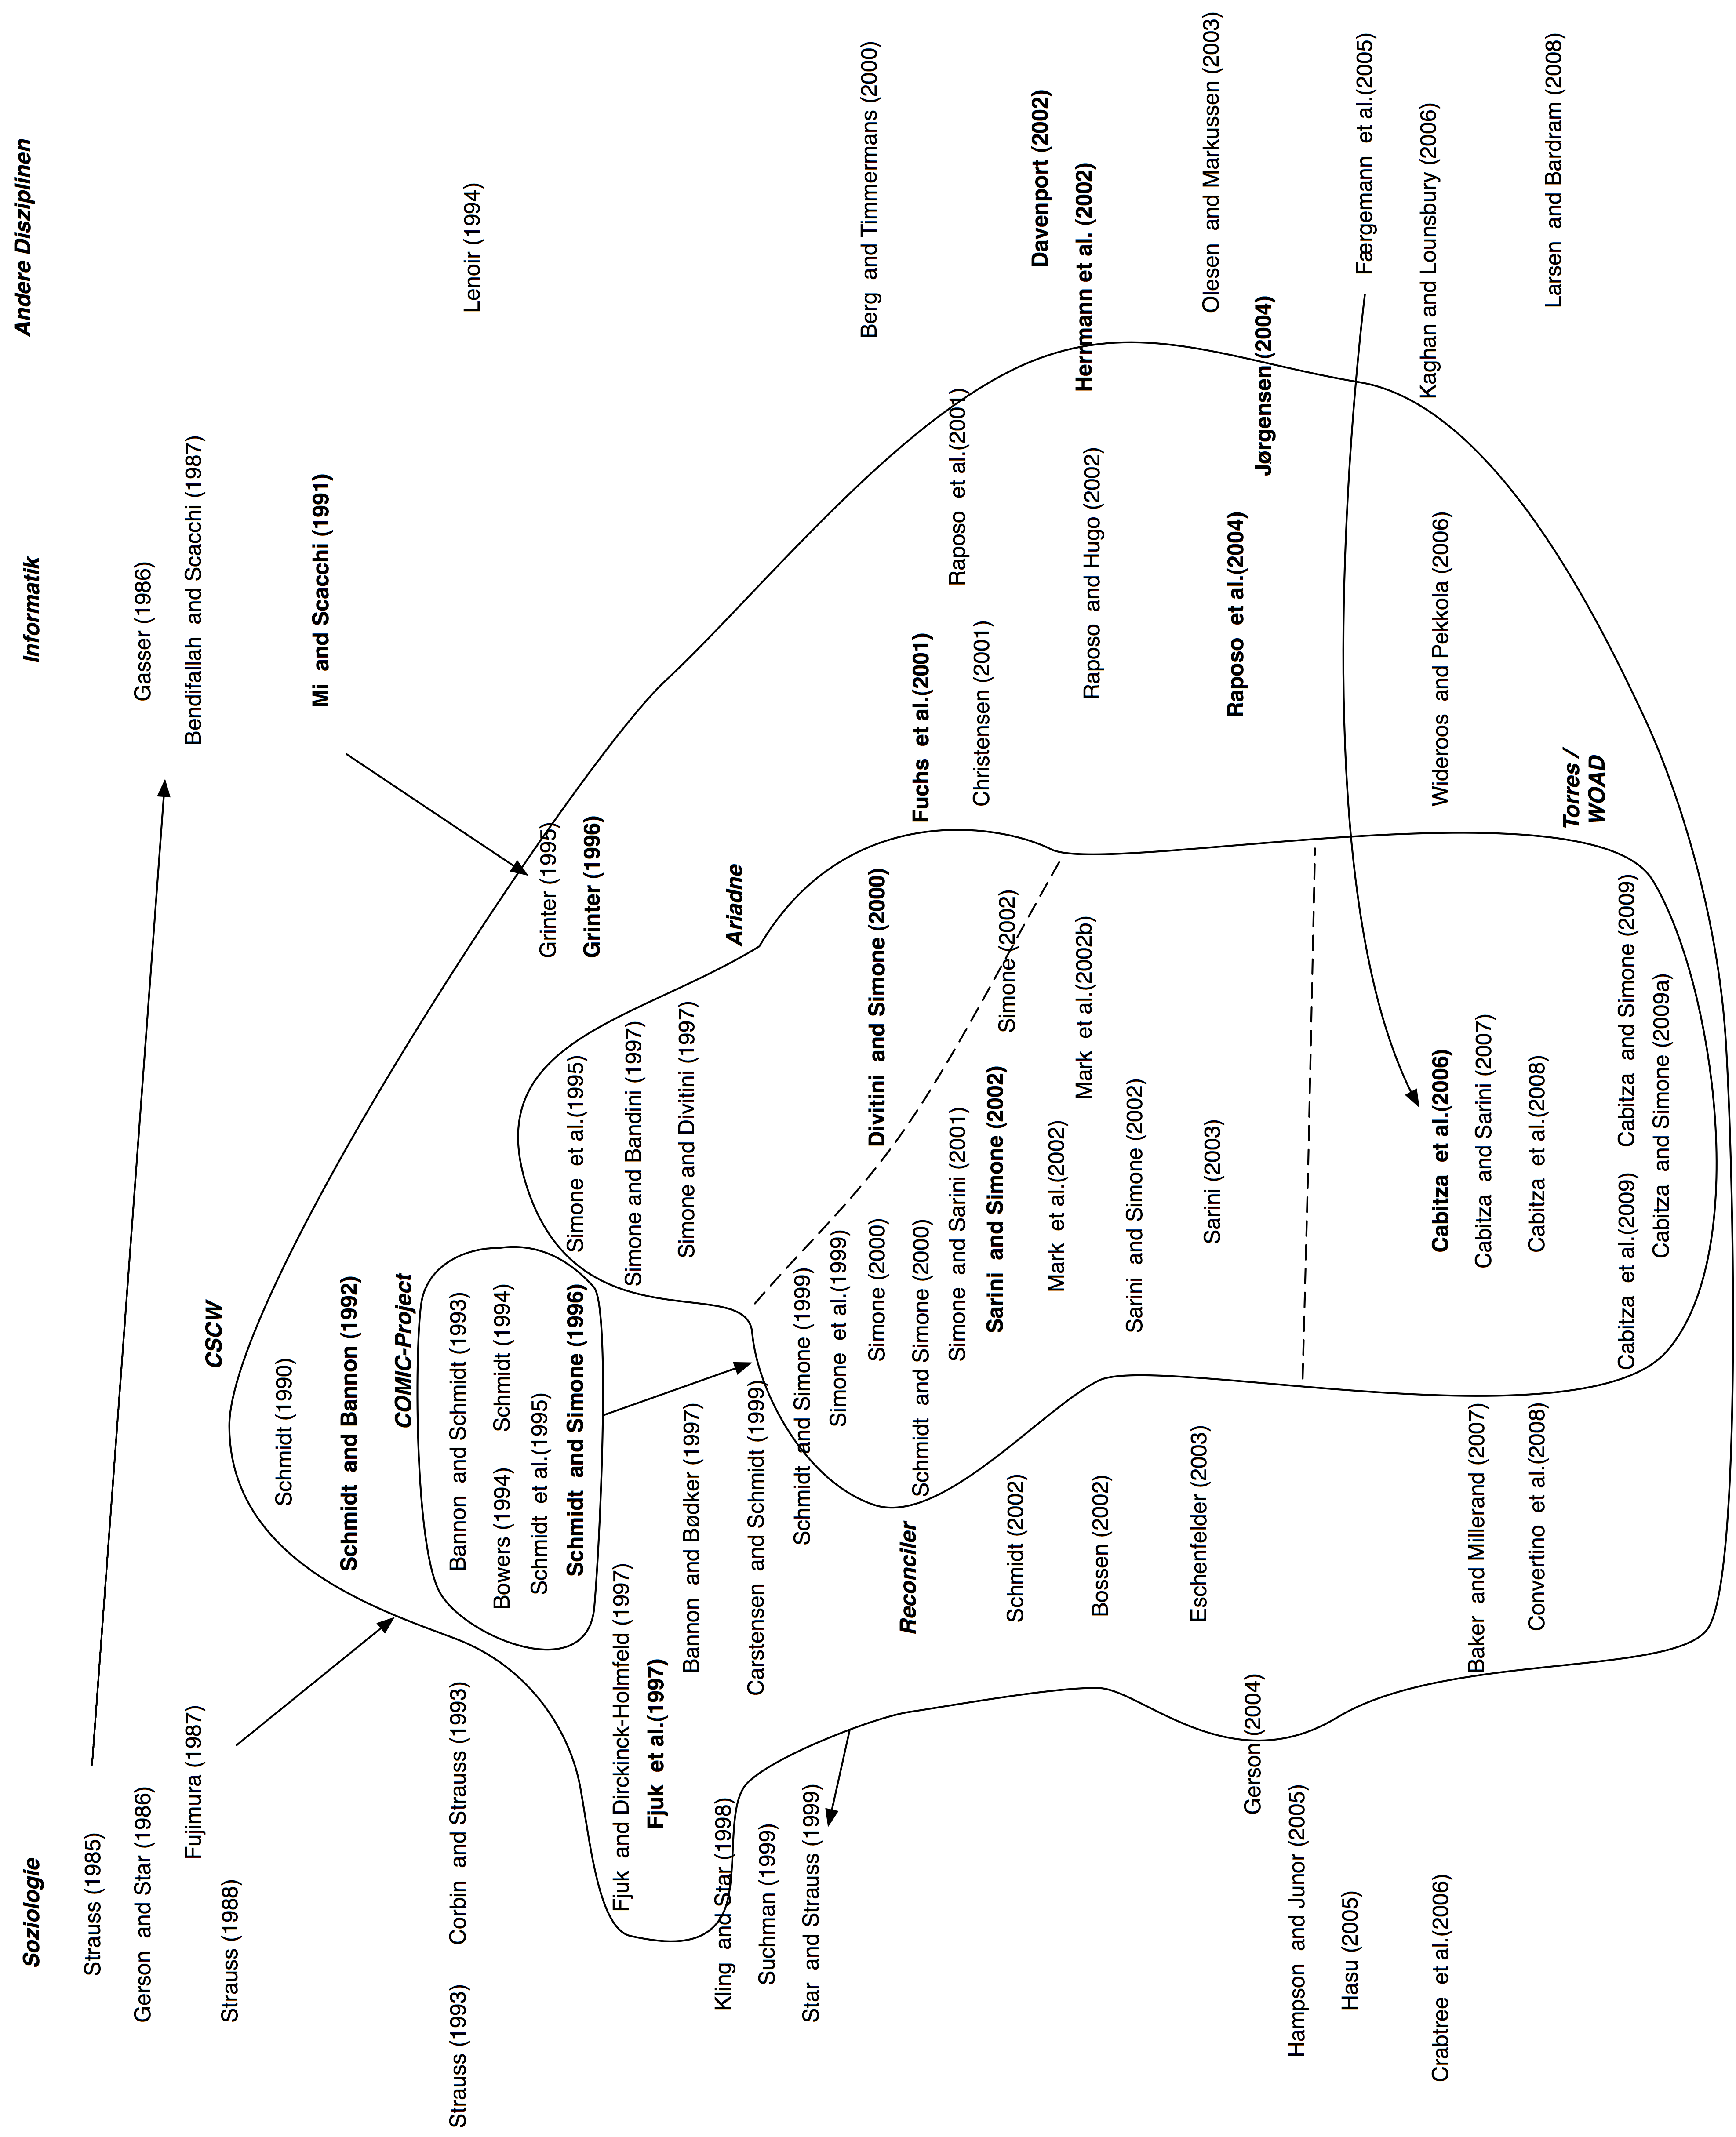
\includegraphics[width=\textwidth]{img/ArticulationWork/ArticulationWorkLiteratur.png}
	\caption{Literatur zu Articulation Work im Kontext}
	\label{fig:img_ArticulationWork_ArticulationWorkLiteratur}
\end{figure}

Beginnend mit den Arbeiten von Strauss in der linken oberen Ecke ist vertikal die zeitliche Dimension der Publikation von Arbeiten zu Artikulation Work aufgetragen. Die Seitenbreite wird zur thematischen Gruppierung der Publikationen verwendet. Die Pfeile zwischen Publikationen bzw. Publikationsgruppen stellen einen inhaltlichen Bezug dar. Die Publikationen am Endpunkt des Pfeils nehmen dabei Bezug auf jene, die sich am Ausgangspunkt des Pfeils befinden.

Am linken Rand der Darstellung sind die Arbeiten zu finden, die im soziologischen Kontext verfasst wurden. Die meisten der dort angesiedelten Publikationen sind Grundlagenarbeiten, die den Begriff „Articulation Work“ und dessen konzeptuellen Kontext erörtern oder anhand von Fallstudien das Auftreten von „Articulation Work“ zeigen.

Im Zentrum der Darstellung steht die größte Gruppe von Arbeiten, die im Kontext von \gls{CSCW} verfasst wurde. Die Arbeiten, die sich auf \gls{CSCW} beziehen, haben dabei zum Teil die Ableitung für Anforderungen an eine technische Unterstützung von „Articulation Work“ zum Ziel, der Rest der Arbeiten beschäftigt sich eher mit der technischen Umsetzung der Unterstützung. Jene Publikationen, die eher ersterer Gruppe zuzuordnen sind, sind eher links angeordnet, die technisch orientierten Publikationen befinden sich eher rechts. Die Entfernung zur Mittelachse hat dabei keine Aussagekraft, sondern ist nur einer übersichtlichen Anordnung geschuldet. 

Innerhalb der \gls{CSCW}-Gruppe gibt es zwei bedeutende Sub-Gruppen, die untereinander in Beziehung stehen. Einerseits ist die Gruppe von Publikationen zu nennen, die im Rahmen des COMIC-Projektes 1992-1995 entstanden sind \citep{Rodden95}. In diesem Projekt wurde die Grundlage der Berücksichtigung von „Articulation Work“ als Thema von \gls{CSCW} gelegt. Bereits im Rahmen des COMIC-Projektes beginnend, publiziert die Gruppe um \citeauthor{Simone00} Arbeiten zur konkreten technischen Umsetzung der Unterstützung durch computerbasierte Werkzeuge. Die Implementierungen, auf die dabei immer wieder Bezug genommen wird, werden als „Ariadne“ (für den Koordinierungsaspekt von „Articulation Work“) „Reconciler“ (für den Awareness-Aspekt von „Articulation Work“) bezeichnet, was auch als Namensgeber dieser Gruppe von Arbeiten herangezogen wurde.

Weiter rechts am oberen Rand der Abbildung befinden sich Arbeiten, die „Articulation Work“ im Kontext der Software-Entwicklung betrachten. Dies sind die ersten Arbeiten, die eine konkrete Anwendung der Konzepte um „Articulation Work“ außerhalb der Soziologie bzw. der Community um Strauss zeigen. Die Unterstützung von „Articulation Work“ ist hier nur teilweise Gegenstand der Betrachtung, wo sie aber angesprochen wird, ist sie entsprechend der Anwendungsdomäne eher technisch orientiert.

Ganz rechts sind jene Arbeiten zu finden, die auf „Articulation Work“ Bezug nehmen, jedoch nicht einer der bisher beschriebenen Gruppen zuzuordnen sind. Hier finden sich Publikationen, die vor philosophischem, organsationswissenschaftlichem Hintergrund oder mit Bezug zum Wissensmanagement verfasst wurden. Herauszugreifen ist hier die Arbeit von \citet{Jorgensen04}, der die Rolle von Modellen (konkret konzeptuellen Modellen von Arbeit) bei der Durchführung von „Articulation Work“ betrachtet und damit erstmals einen konkreten Unterstützungsbezug zwischen „Artikulation Work“ und der Domäne der Organisationswissenschaften herstellt (was wiederum für die Betrachtung von „Articulation Work“ im organisationalen Kontext von Interesse ist).

Insgesamt ist in der Abbildung ein starker Schwerpunkt auf die technische Unterstützung von Arbeit, konkret „Articulation Work“, zu erkennen. Dieser Schwerpunkt wurde sowohl konzeptuell als auch technisch ab Beginn der 90er-Jahre des 20. Jahrhunderts bis etwa 2005 ausführlich bearbeitet. In den letzten Jahren treten verstärkt Fallstudien auf, die einen Bezug zu „Articulation Work“ herstellen, jedoch nur bedingt auf deren Unterstützung eingehen.

% section relevante_literatur (end)

% chapter literatur_zum_themengebiet_articulation_work (end)

\chapter{Daten der empirischen Untersuchung} % (fold)
\label{cha:daten_der_empirischen_untersuchung}

Die Darstellung der erhobenen Rohdaten der empirischen Untersuchung und deren detaillierte Auswertung würden an dieser Stelle den Rahmen der Arbeit sprengen. Durch die große Anzahl an Videoaufnahmen, die insgesamt etwa XY \gls{GB} an Platzbedarf einnehmen, ist auch die Beilage eines Datenträgers nicht möglich. 

Die Rohdaten, die durchgeführten Auswertungen und Transkripte sowie die Skripte der statistischen Tests mit der Software R können via eMail unter

\begin{center} stefan@oppl.info \end{center}

angefordert werden. 

\section{Verfügbare Rohdaten} % (fold)
\label{sec:verfügbare_rohdaten}

Zu den Untersuchungen stehen im Einzelnen folgende Rohdaten zur Verfügung:
\begin{itemize}
	\item Evaluierungsblock 1 (siehe auch \citep{Bohninger10})
		\begin{itemize}
			\item Videoaufnahmen der Modellbildung (Detailansicht der Modellierungsoberfläche)
			\item Fotos der finalen Versionen der erstellten Modelle
		\end{itemize}
	\item Evaluierungsblock 2
		\begin{itemize}
			\item Videoaufnahmen der Modellbildung aus jeweils 2 Perspektiven (Gesamtübersicht inkl. Personen sowie Detailansicht der Modellierungsoberfläche)
			\item Fotos bzw. Graphische Abbildungen der finalen Versionen der erstellten Modelle
		\end{itemize}
	\item Evaluierungsblock 3
		\begin{itemize}
			\item Videoaufnahmen der Modellbildung aus jeweils 2 Perspektiven (Gesamtübersicht inkl. Personen sowie Detailansicht der Modellierungsoberfläche)
			\item Graphische Abbildungen der finalen Versionen der erstellten Modelle
		\end{itemize}
	\item Evaluierungsblock 4 (siehe auch \citep{Wahlmuller10})
		\begin{itemize}
			\item Videoaufnahmen der Modellbildung können aus Gründen der Schutzes unternehmensinterner Information auf diesem Wege nicht weitergegeben werden. Etwaige Anfragen sind an Patrick Wahlmüller (Kontaktdaten in \citep{Wahlmuller10}) zu richten.
			\item Graphische Abbildungen der finalen Versionen der erstellten Modelle
		\end{itemize}
	\item Evaluierungsblock 5 (siehe auch \citep{Bindreiter10})
		\begin{itemize}
			\item Videoaufnahmen der Modellbildung mittels CMapTools und am Modellierungstisch aus jeweils 2 Perspektiven (Gesamtübersicht inkl. Personen sowie Detailansicht der Modellierungsoberfläche)
			\item Graphische Abbildungen der finalen Versionen der erstellten Modelle
			\item Als XML exportierte Repräsentationen der mit CMapTools erstellten Modelle (inkl. Modellierungshistorie)
			\item Fragebogen 
		\end{itemize}
\end{itemize}

% section verfügbare_rohdaten (end)

\section{Durchgeführte Auswertungen} % (fold)
\label{sec:durchgeführte_auswertungen}

Zu den Untersuchungen wurden folgende Auswertungen durchgeführt und archiviert. Die einzelnen Auswertungsmethoden sind auf den folgenden Seiten näher beschrieben.

\begin{itemize}
	\item Evaluierungsblock 1 (siehe auch \citep{Bohninger10})
		\begin{itemize}
			\item Überblicksauswertung aller Anwendungen und Modelle
			\item  
		\end{itemize}
	\item Evaluierungsblock 2
		\begin{itemize}
			\item Überblicksauswertung aller Anwendungen und Modelle
			\item Interaktionsanalyse aller Anwendungen
		\end{itemize}
	\item Evaluierungsblock 3
		\begin{itemize}
			\item Überblicksauswertung aller Anwendungen und Modelle
			\item Interaktionsanalyse aller Anwendungen
		\end{itemize}
	\item Evaluierungsblock 4 (siehe auch \citep{Wahlmuller10})
		\begin{itemize}
			\item Überblicksauswertung aller Anwendungen und Modelle
			\item Interaktionsanalyse aller Anwendungen
		\end{itemize}
	\item Evaluierungsblock 5 (siehe auch \citep{Bindreiter10})
		\begin{itemize}
			\item Überblicksauswertung aller Anwendungen und Modelle
			\item Interaktionsanalyse aller Anwendungen
		\end{itemize}
\end{itemize}

\subsection{Überblicksauswertung}

Die Überblicksauswertung fasst die wesentlichen Eigenschaften des in einer Anwendung erstellten Modells sowie die während der Erstellung aufgetretenen Ereignisse zusammen. Die Daten wurden in Form einer Openoffice-Tabelle aufbereitet und stehen als \gls{ODF}-Dateien zur Verfügung. Sie dienen als Grundlage aller weiteren deskriptiven und schließenden statistischen Auswertungen.

Die konkrete Ausgestaltung der Tabelle variiert je nach Evaluierungsblock (abhängig von der durchgeführten Modellierungsaufgabe und der im Werkzeug implementierten Funktionalität) leicht, in Abbildung \ref{fig:img_AnhangEmpirie_raster} ist der Raster aus Evaluierungsblock 5 dargestellt, in dem die höchste Anzahl von Merkmalen erhoben wurden.

\begin{figure}[htbp]
	\centering
		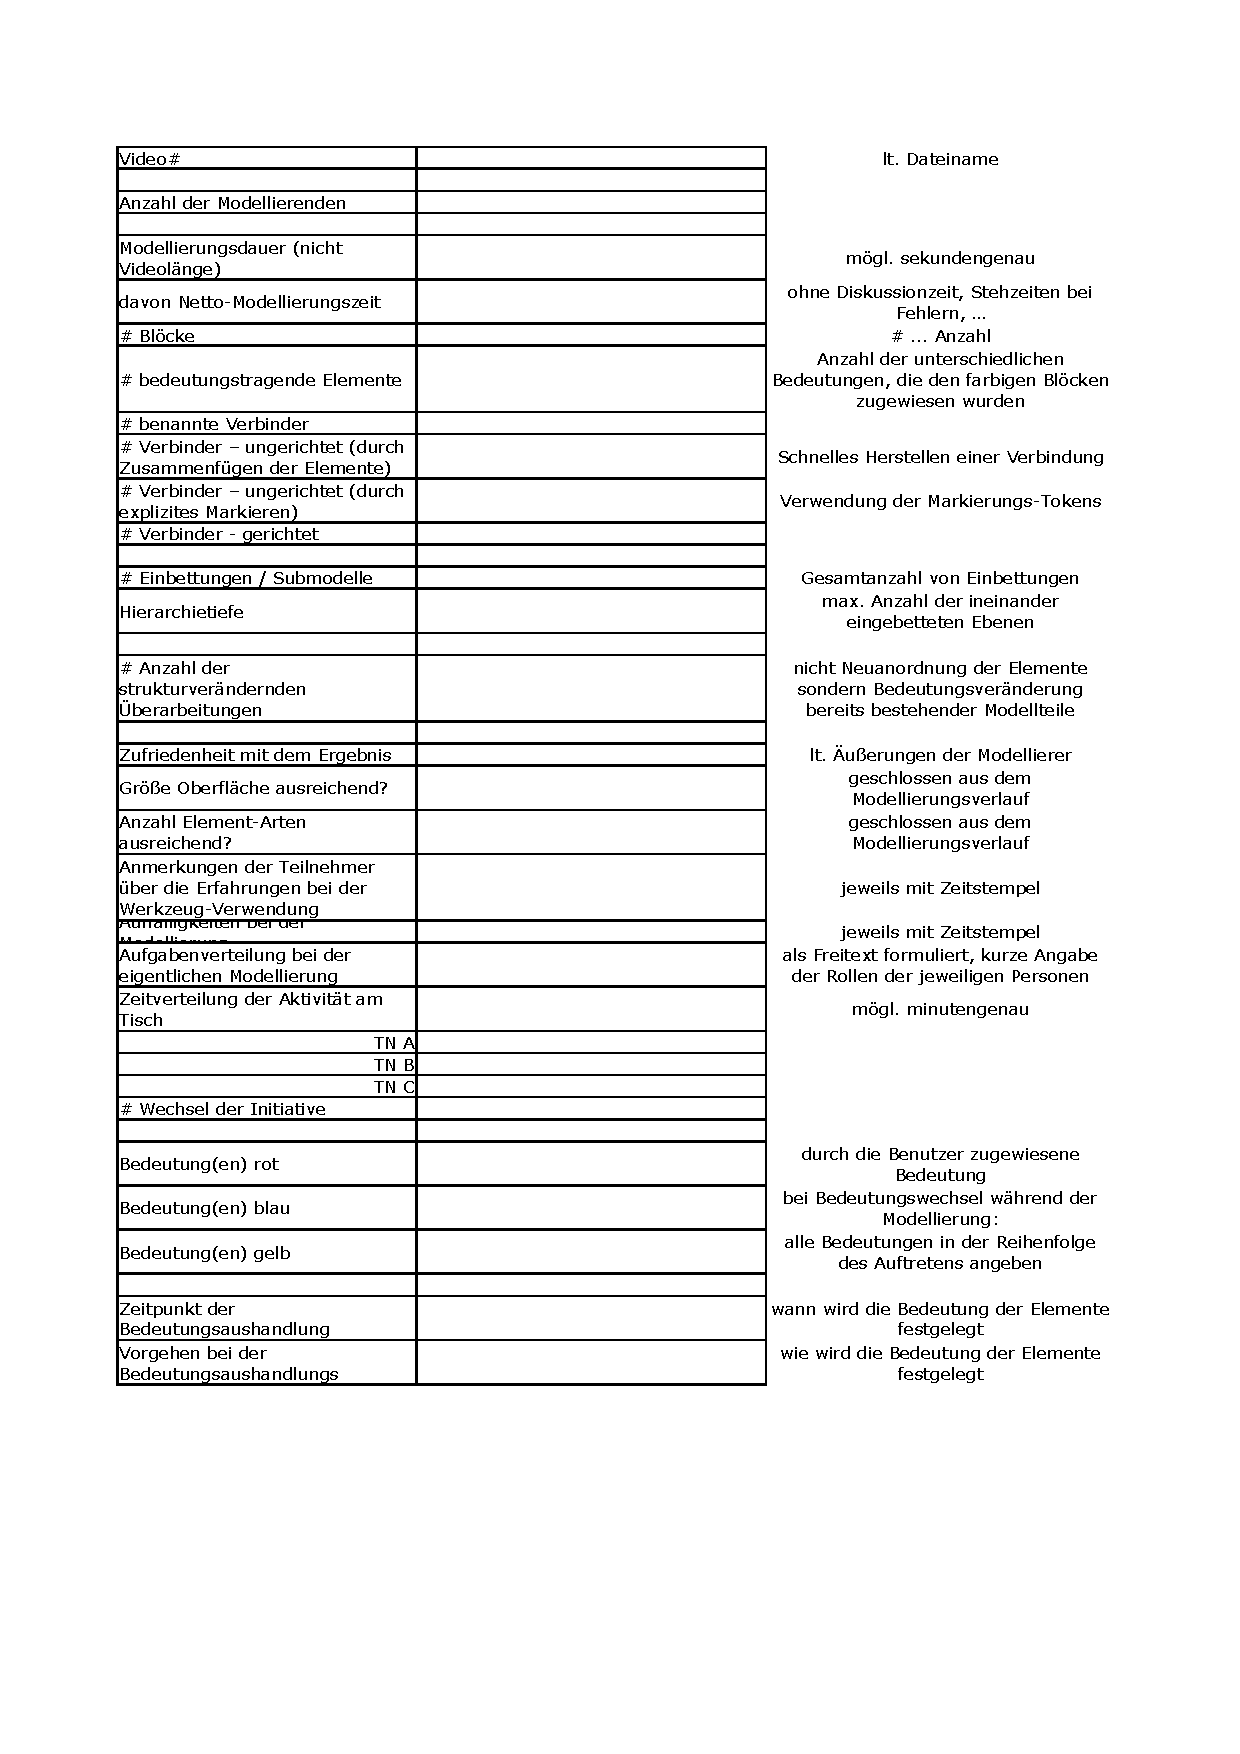
\includegraphics[width=0.9\textwidth]{img/AnhangEmpirie/raster.pdf}
	\caption{Raster der Überblicksauswertung}
	\label{fig:img_AnhangEmpirie_raster}
\end{figure}

Die Befüllung der Raster erfolgte auf Basis der angefertigten Video-Aufnahmen der Werkzeuganwendungen. In den Blöcken 3 und 5 wurden die Raster redundant unabhängig voneinander von jeweils zwei Personen befüllt. Sofern Abweichungen bei der Auswertung der quantitativen Parameter festgestellt wurden, wurde das jeweilige Merkmal durch eine dritte Person geprüft und ggf. entsprechend korrigiert. In den Blöcken 1, 2 und 4 standen nicht ausreichend personelle Ressourcen für eine redundante Auswertung zur Verfügung.

\subsection{Interaktionsanalyse}

Die Interaktionsanalyse wurde wie in Abschnitt \ref{sub:interaktionsanalyse} beschrieben durchgeführt und dokumentiert. Die Dokumentation erfolgte in Textdokumenten, die als \gls{ODF}-Dateien zur Verfügung stehen.

In den Evaluierungsblöcken 3 und 5 wurde die Interaktionsanalyse für jede Werkzeuganwendung von zwei Personen redundant durchgeführt. In den Blöcken 2 und 4 standen die personellen Ressourcen für eine redundante Auswertung nicht zur Verfügung. In den Fällen, in denen redundant ausgewertet wurde, wurden Transkripte, die nur von einer der auswertenden Personen erfasst wurden, von einer dritten Person geprüft und bestätigt bzw. verworfen.

% section durchgeführte_auswertungen (end)

\section{Verwendete Fragebögen} % (fold)
\label{sec:frageboegen}

Bei der Durchführung der Evaluierungsblöcke 1, 4 und 5 wurden zusätzlich zu den direkt aus der Modellbildung erhobenen Daten auch Benutzerbefragungen mittels Fragebögen durchgefürht. Im Folgenden sind für jeden Evaluierungsblock die verwendeten Fragebögen angeführt. Zusätzlich werden die Fragebögen hinsichlich ihrer Relevanz für die untersuchten Hypothesen (siehe Kapitel \ref{cha:eval_werkzeug} bis \ref{cha:eval_aw}) eingeordnet. Die Auswertungen der ausgefüllten Fragebögen sind in digitaler Form detailliert (siehe Abschnitt \ref{sec:verfügbare_rohdaten}) bzw. aggregiert (siehe Abschnitt \ref{sec:durchgeführte_auswertungen}) in digitaler Form verfügbar.


\fboxrule0.4mm
\fboxsep0.1mm

\subsection{Fragebögen aus Evaluierungsblock 1}
\label{sub:fb_eval1}

Die Abbildungen \ref{fig:img_AnhangEmpirie_fb5-01} bis \ref{fig:img_AnhangEmpirie_fb5-05} zeigen den in Evaluierungsblock 1 verwendeten Fragebogen. Der Aufbau des Fragebogens wurde von \cite{Bohninger10} detailliert beschrieben und begründet.

\subsection{Fragebögen aus Evaluierungsblock 4}
\label{sub:fb_eval4}

Die Abbildungen \ref{fig:img_AnhangEmpirie_fb5-01} bis \ref{fig:img_AnhangEmpirie_fb5-05} zeigen den in Evaluierungsblock 4 verwendeten Fragebogen. Der Aufbau des Fragebogens wurde von \citet{Wahlmuller10} detailliert beschrieben und begründet.


\subsection{Frageböqgen aus Evaluierungsblock 5}
\label{sub:fb_eval5}

Die Abbildungen \ref{fig:img_AnhangEmpirie_fb5-01} bis \ref{fig:img_AnhangEmpirie_fb5-05} zeigen den in Evaluierungsblock 5 verwendeten Fragebogen. Der Aufbau des Fragebogens wurde von \citet{Bindreiter10} detailliert beschrieben und begründet.

\begin{figure}[htbp]
	\centering
	\fbox{%
		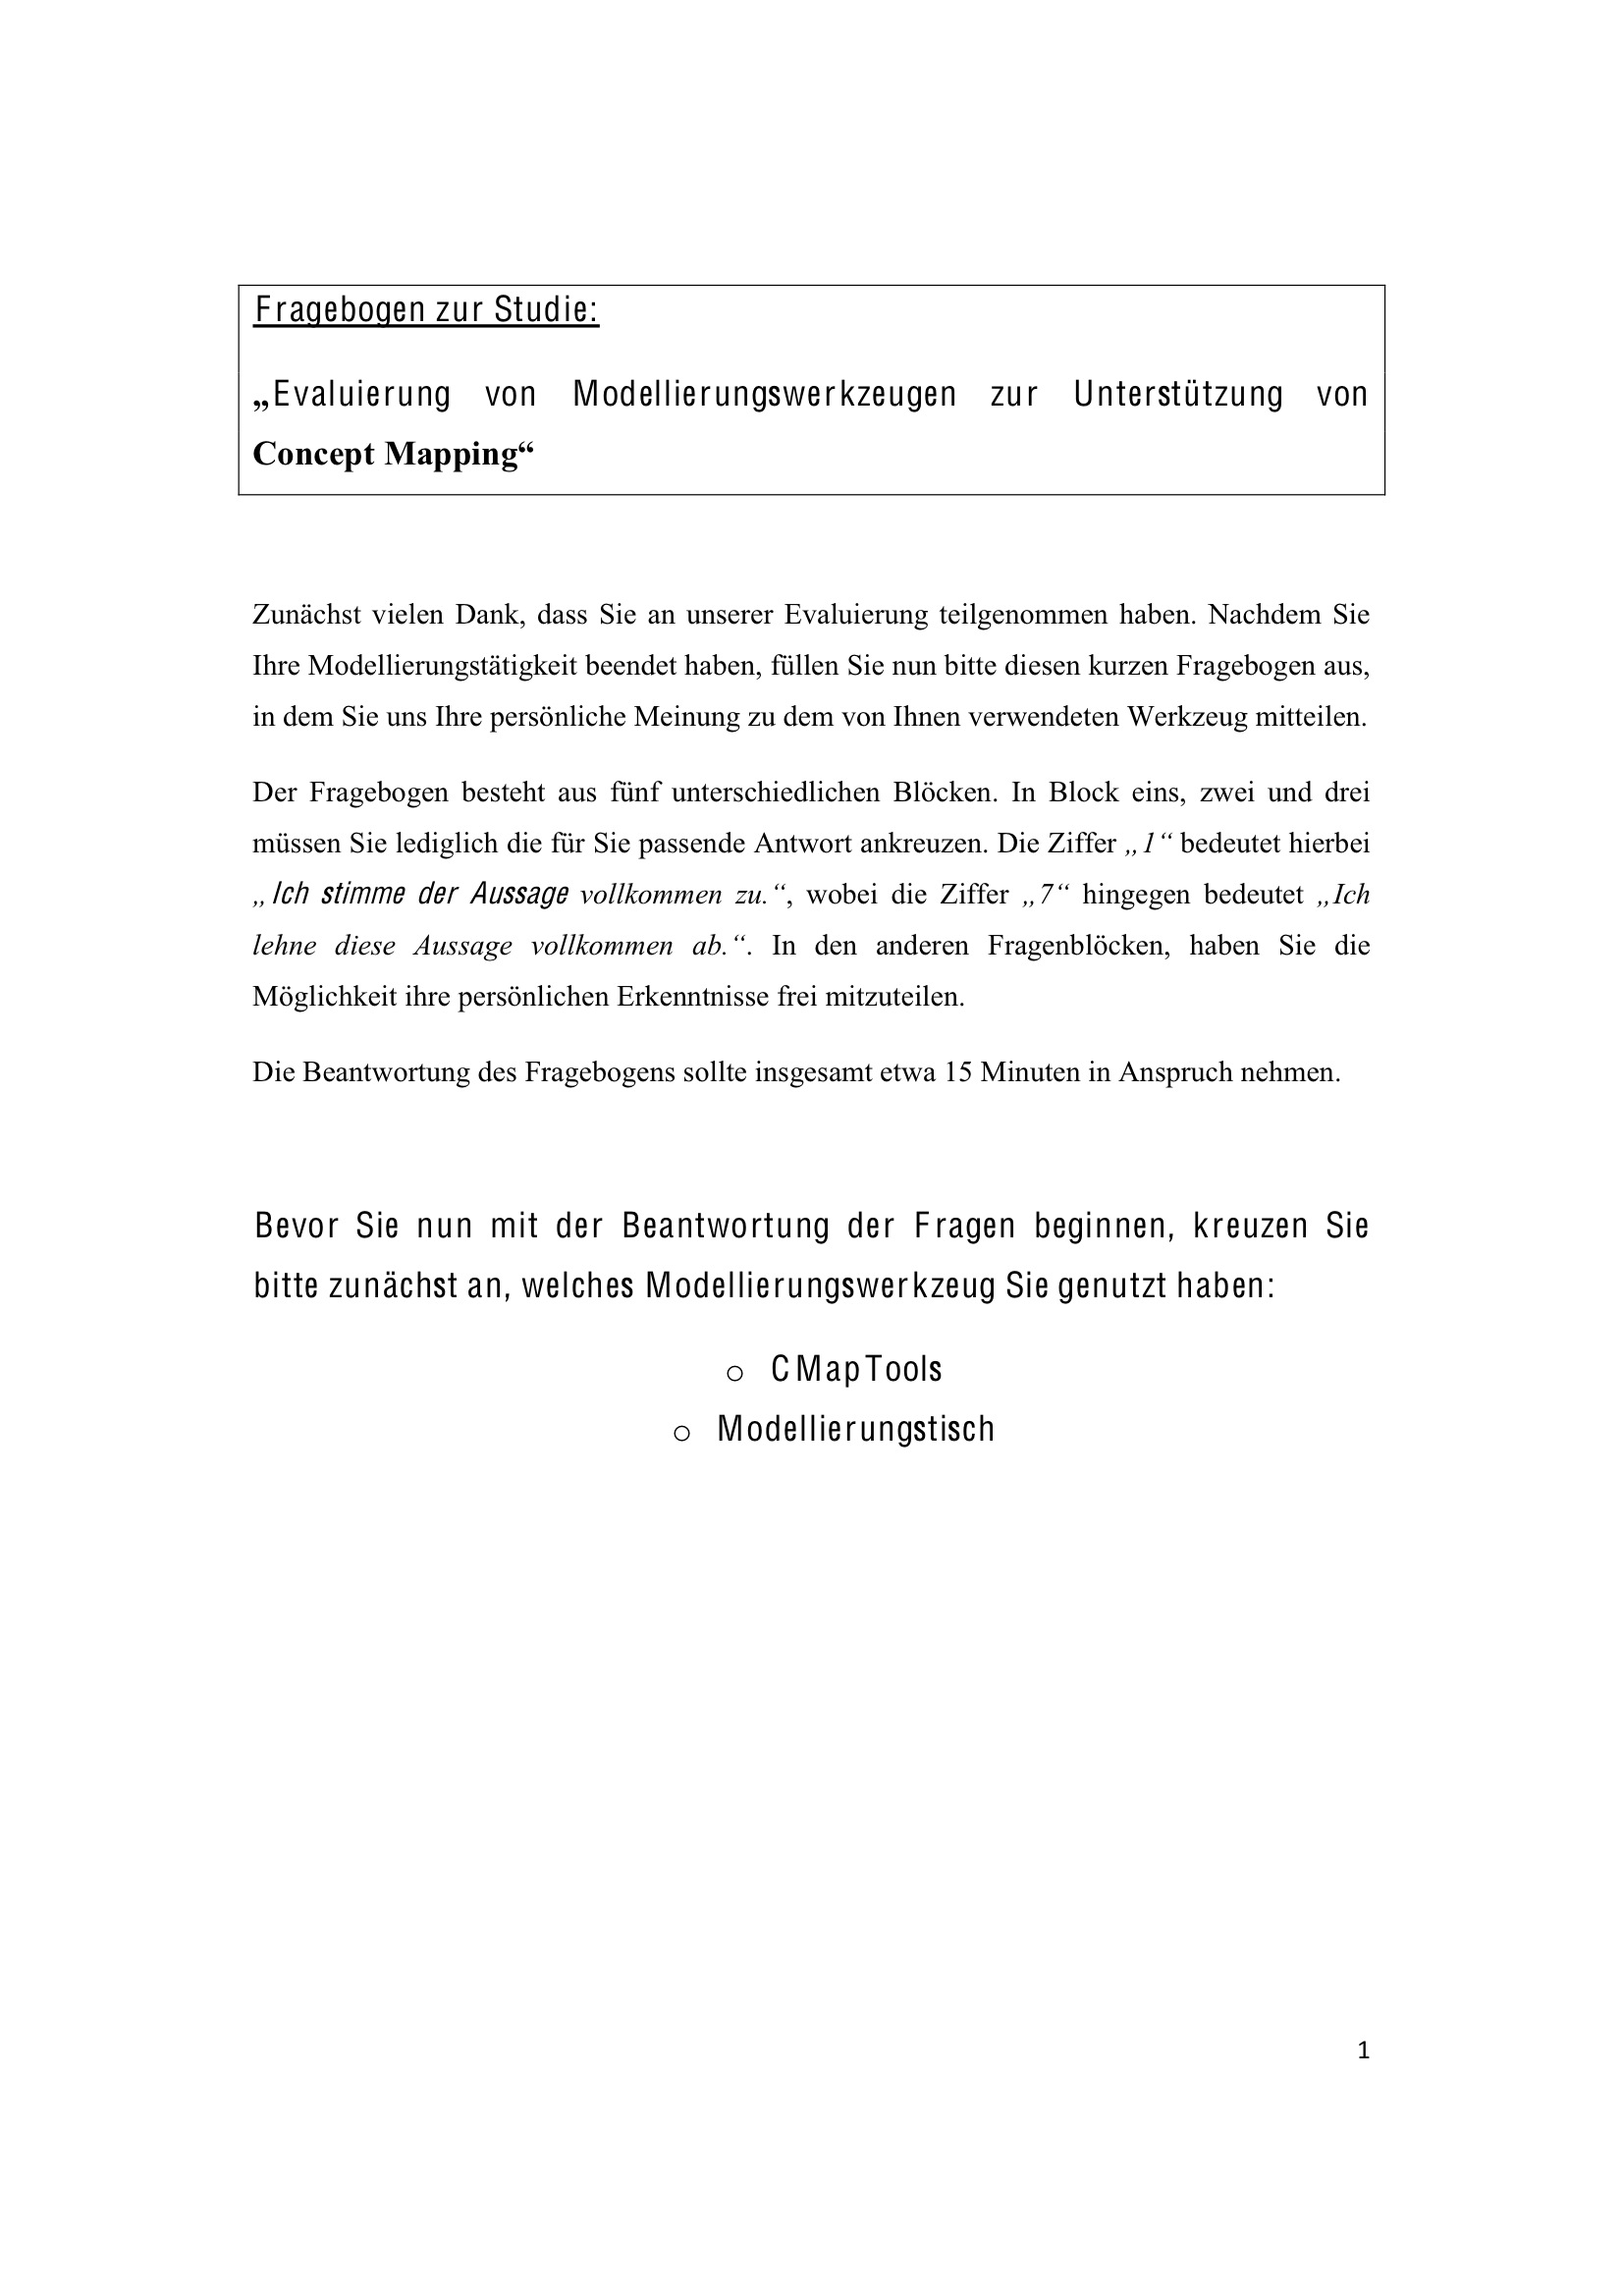
\includegraphics[width=0.9\textwidth]{img/AnhangEmpirie/fb5-01.jpeg}%
	}
	\caption{Fragebogen für Evaluierungsblock 5 - Seite 1}
	\label{fig:img_AnhangEmpirie_fb5-01}
\end{figure}

\begin{figure}[htbp]
	\centering
	\fbox{%
		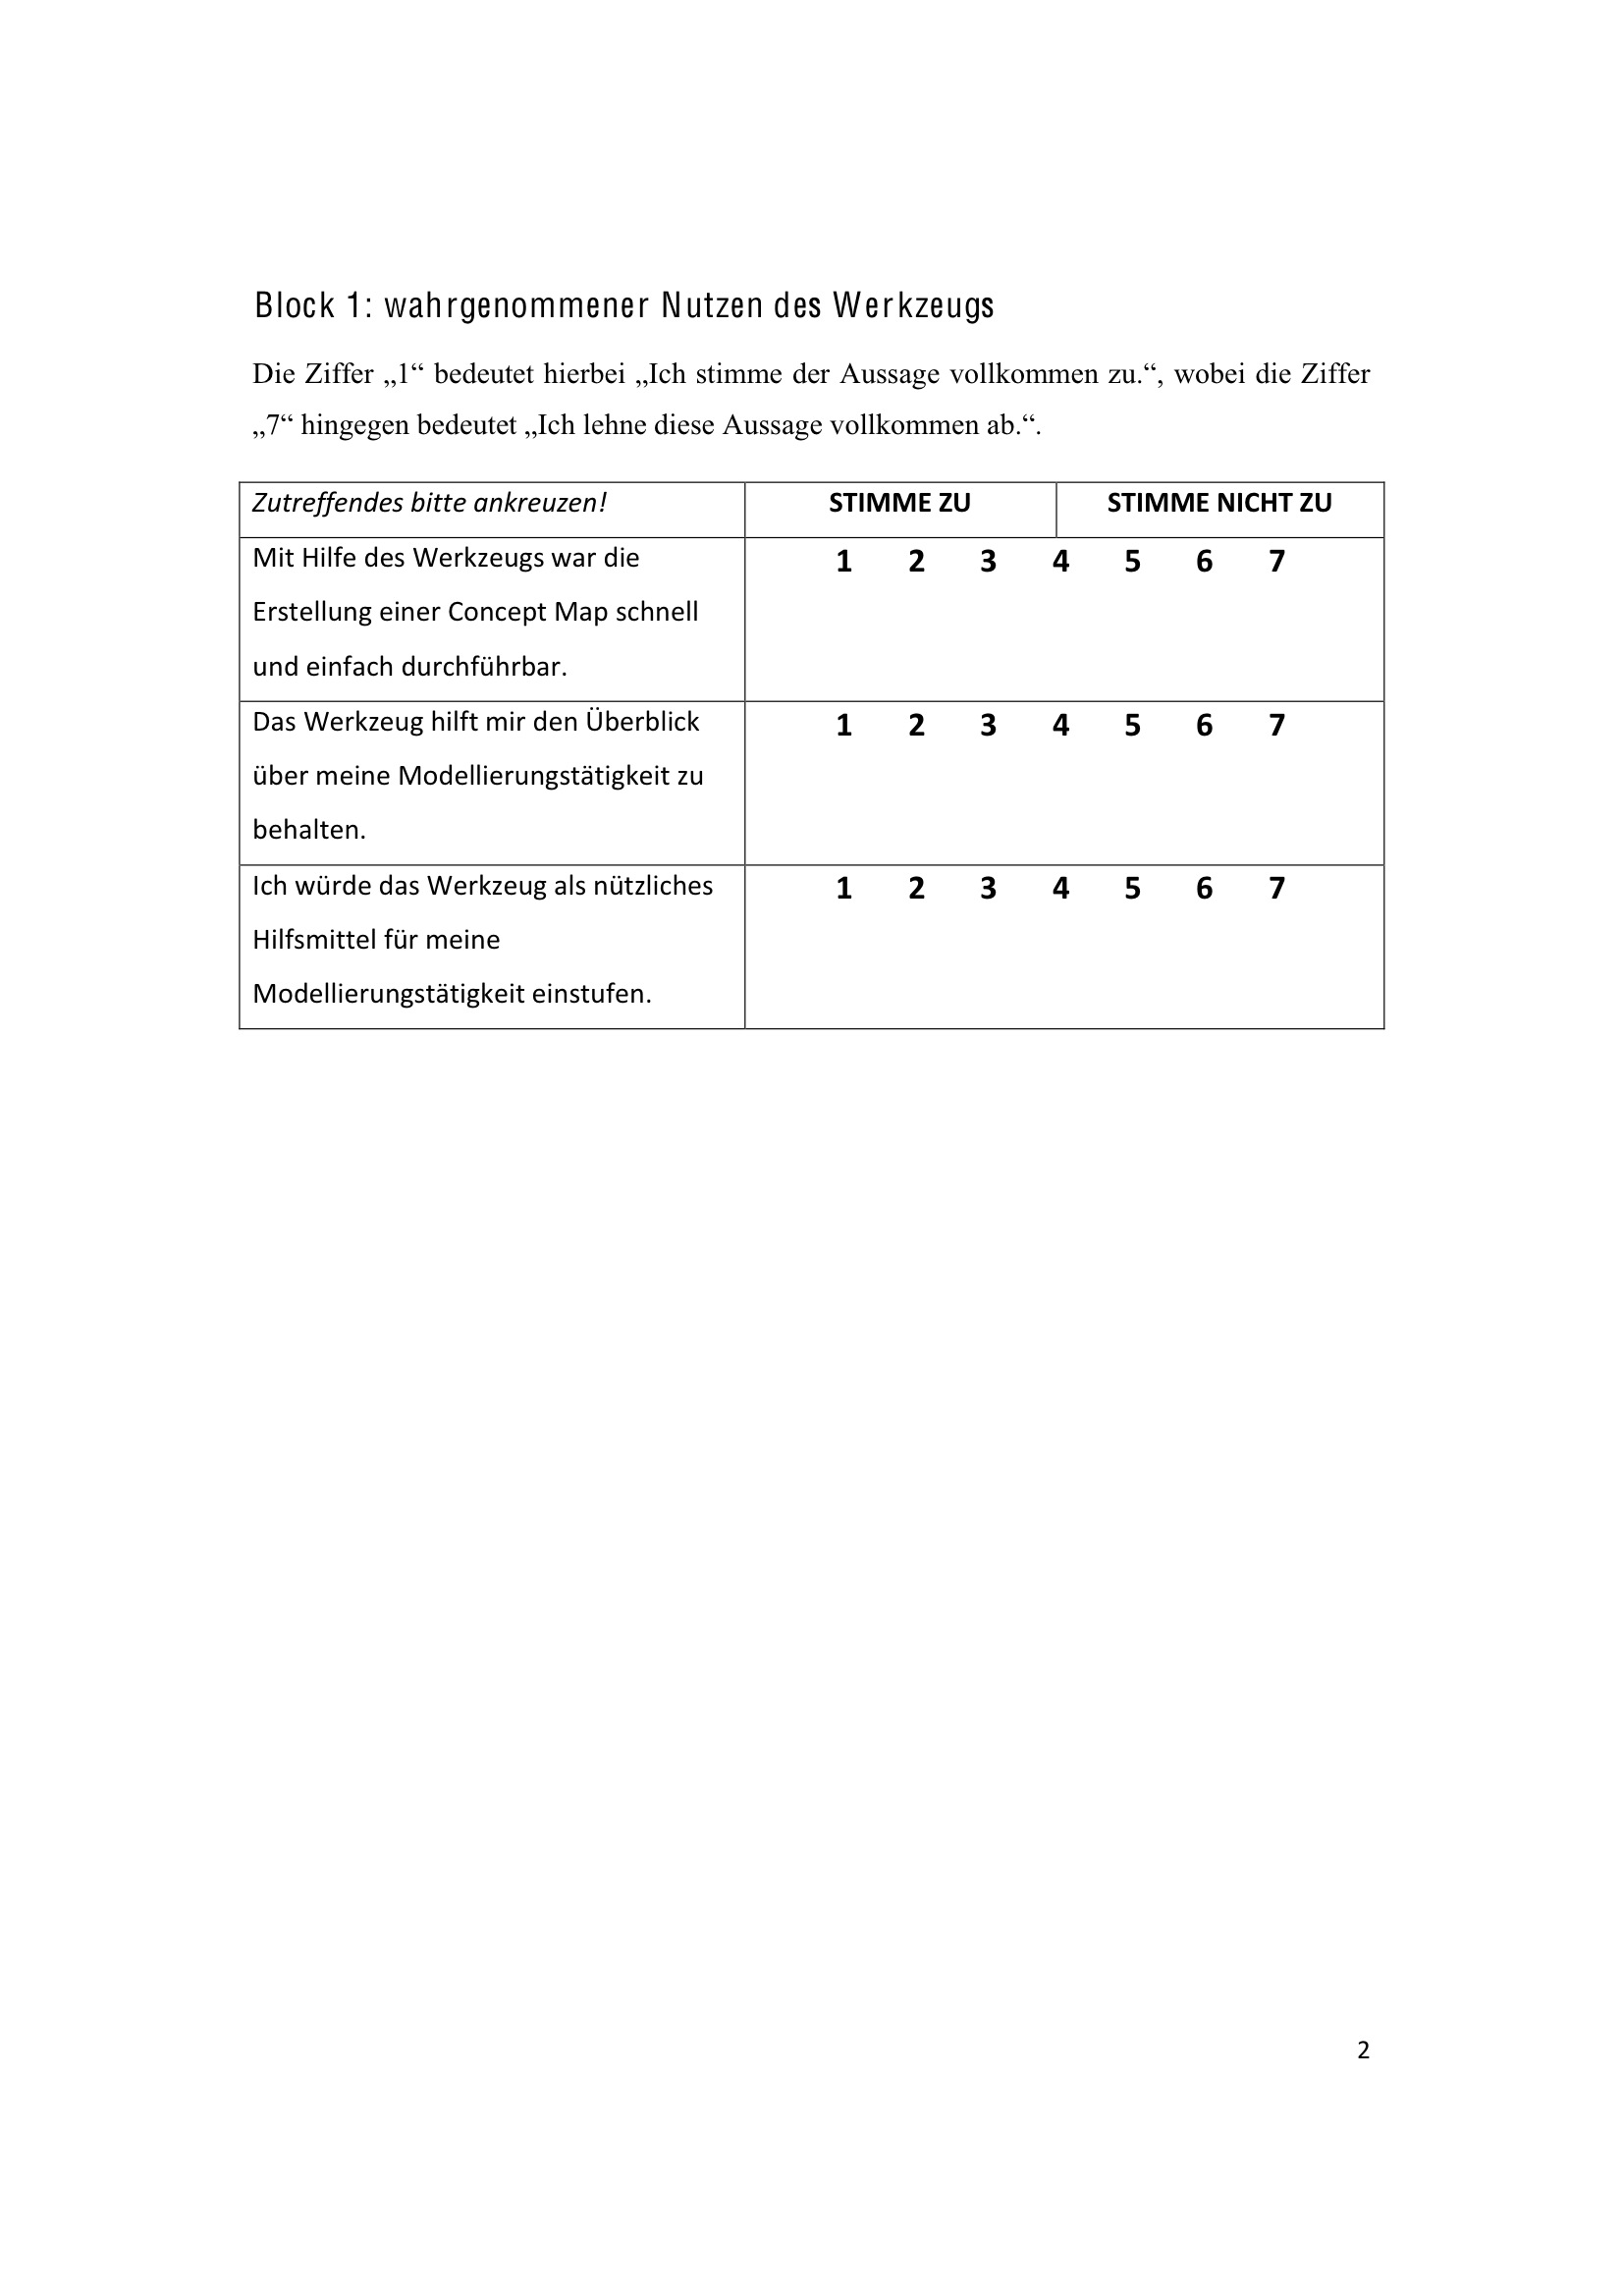
\includegraphics[width=0.9\textwidth]{img/AnhangEmpirie/fb5-02.jpeg}%
	}
	\caption{Fragebogen für Evaluierungsblock 5 - Seite 2}
	\label{fig:img_AnhangEmpirie_fb5-02}
\end{figure}

\begin{figure}[htbp]
	\centering
	\fbox{%
		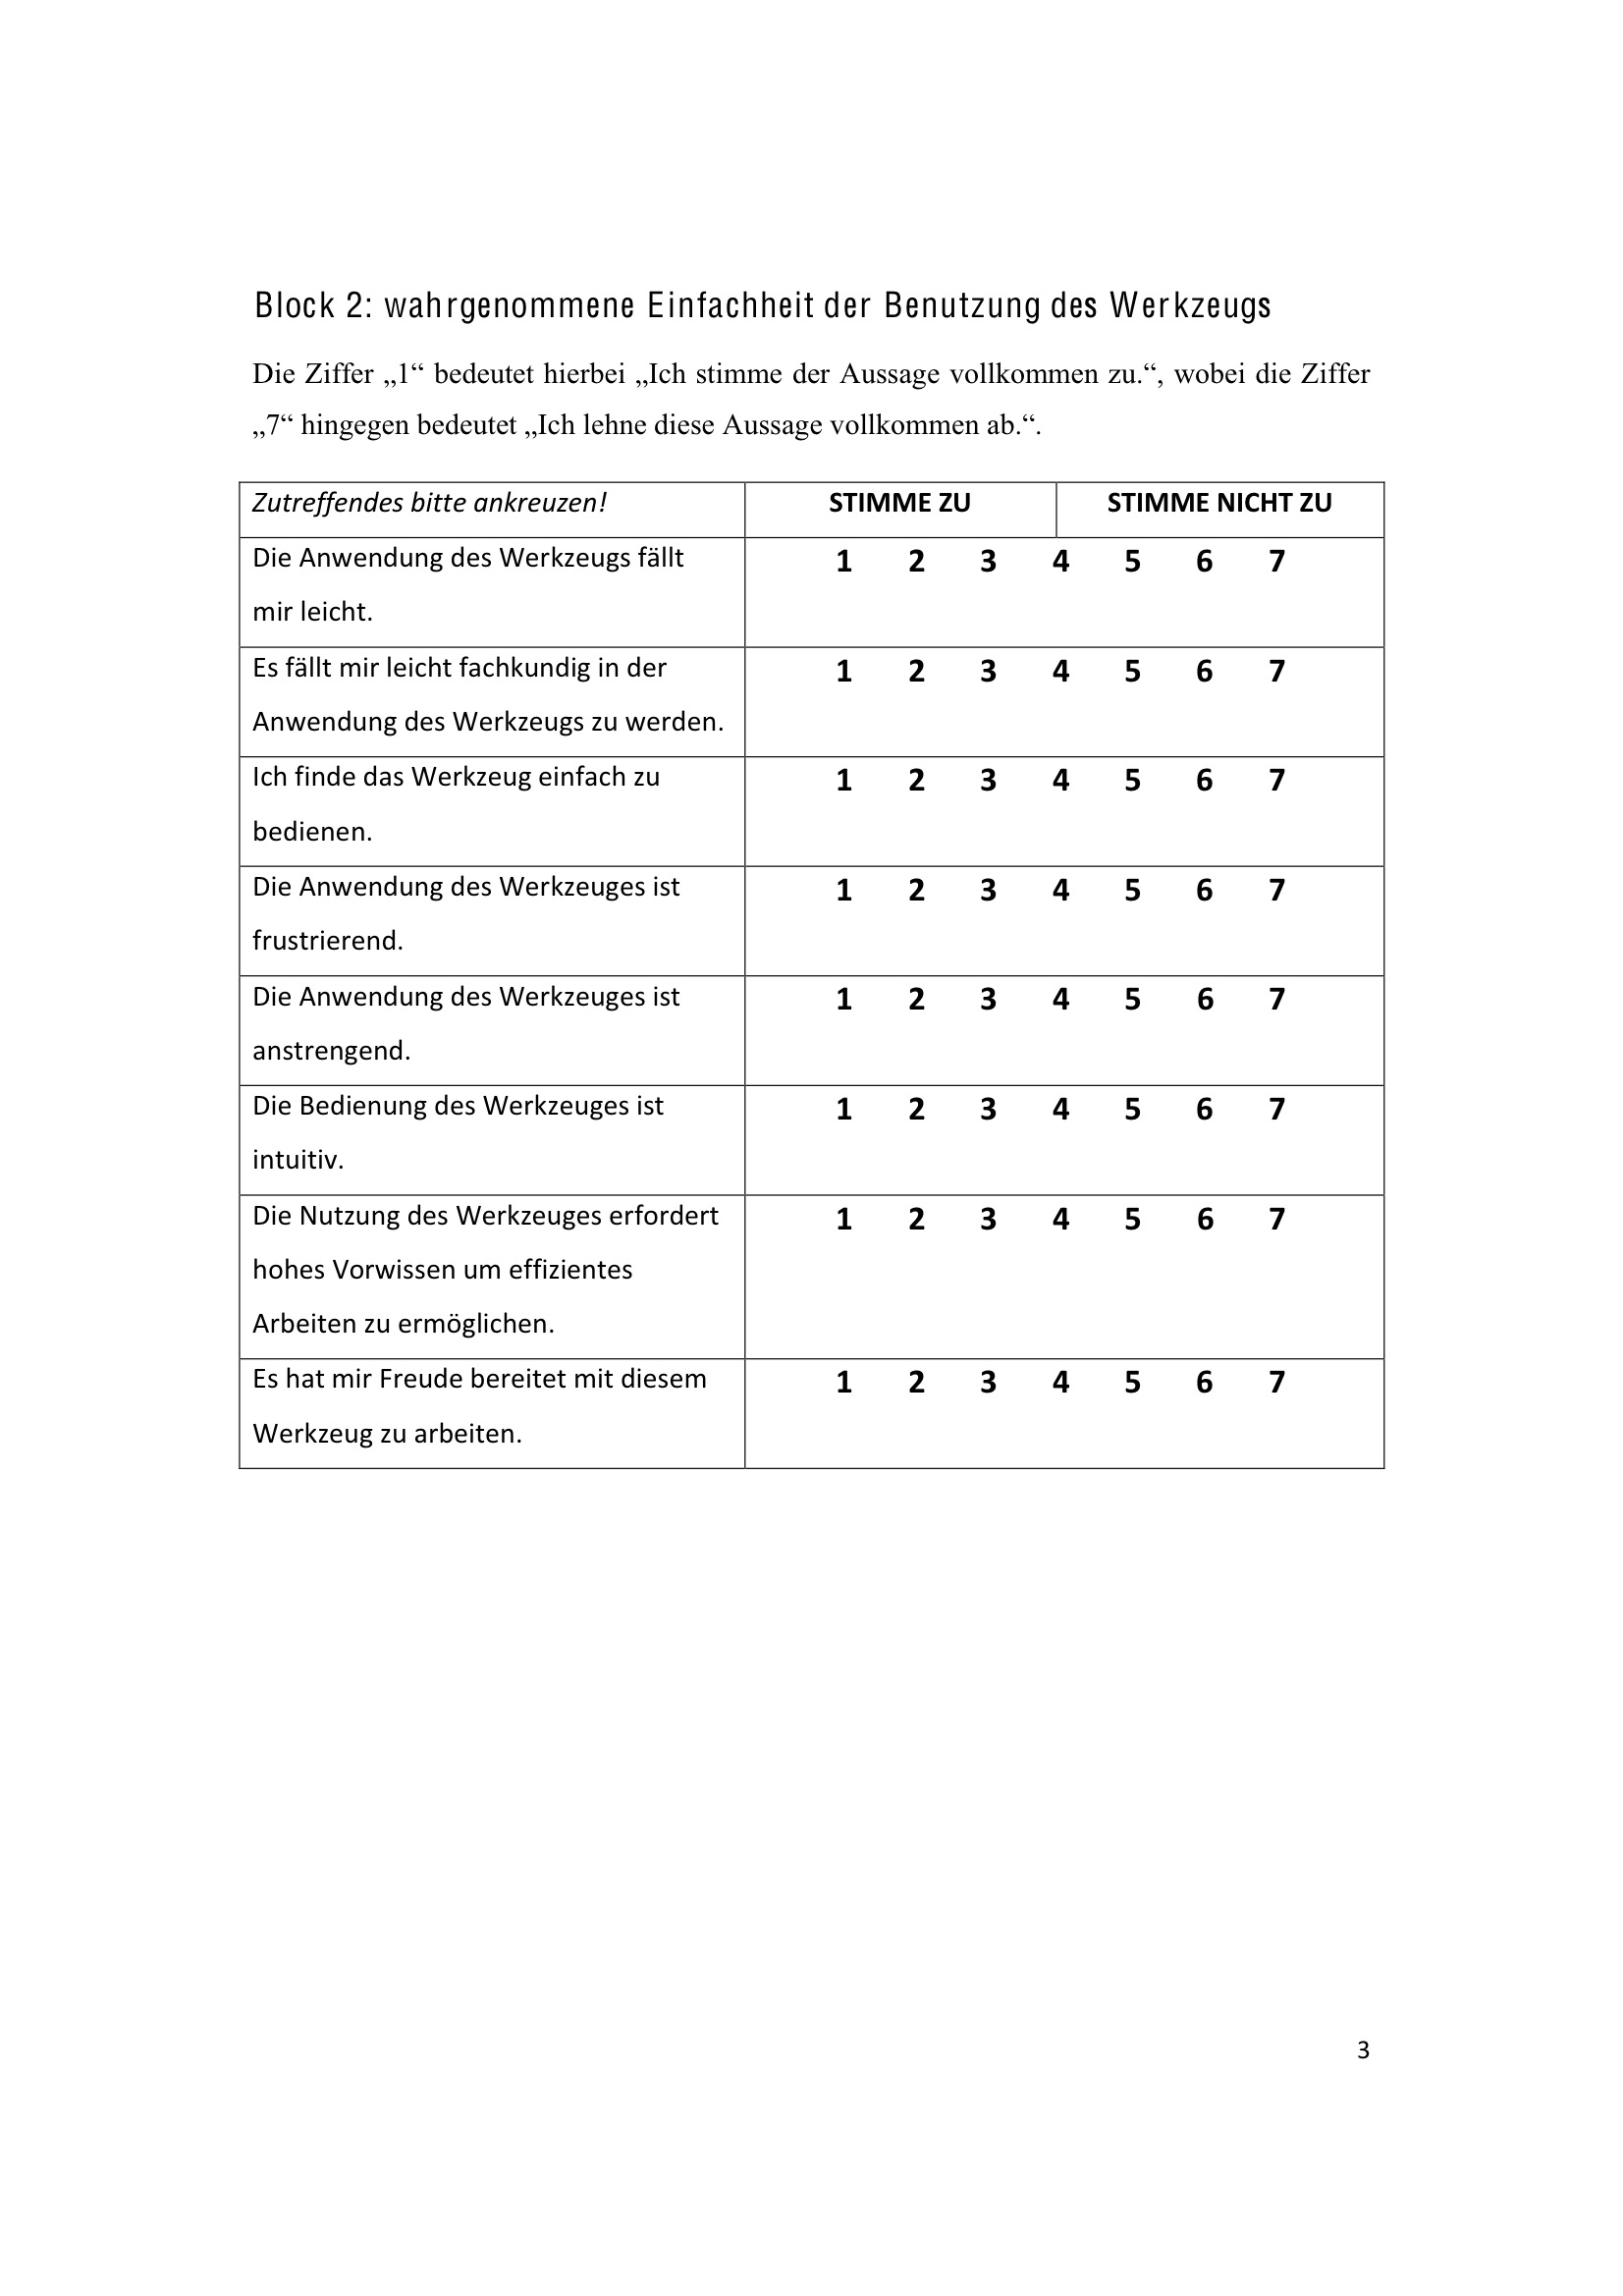
\includegraphics[width=0.9\textwidth]{img/AnhangEmpirie/fb5-03.jpeg}%
	}
	\caption{Fragebogen für Evaluierungsblock 5 - Seite 3}
	\label{fig:img_AnhangEmpirie_fb5-03}
\end{figure}

\begin{figure}[htbp]
	\centering
	\fbox{%
		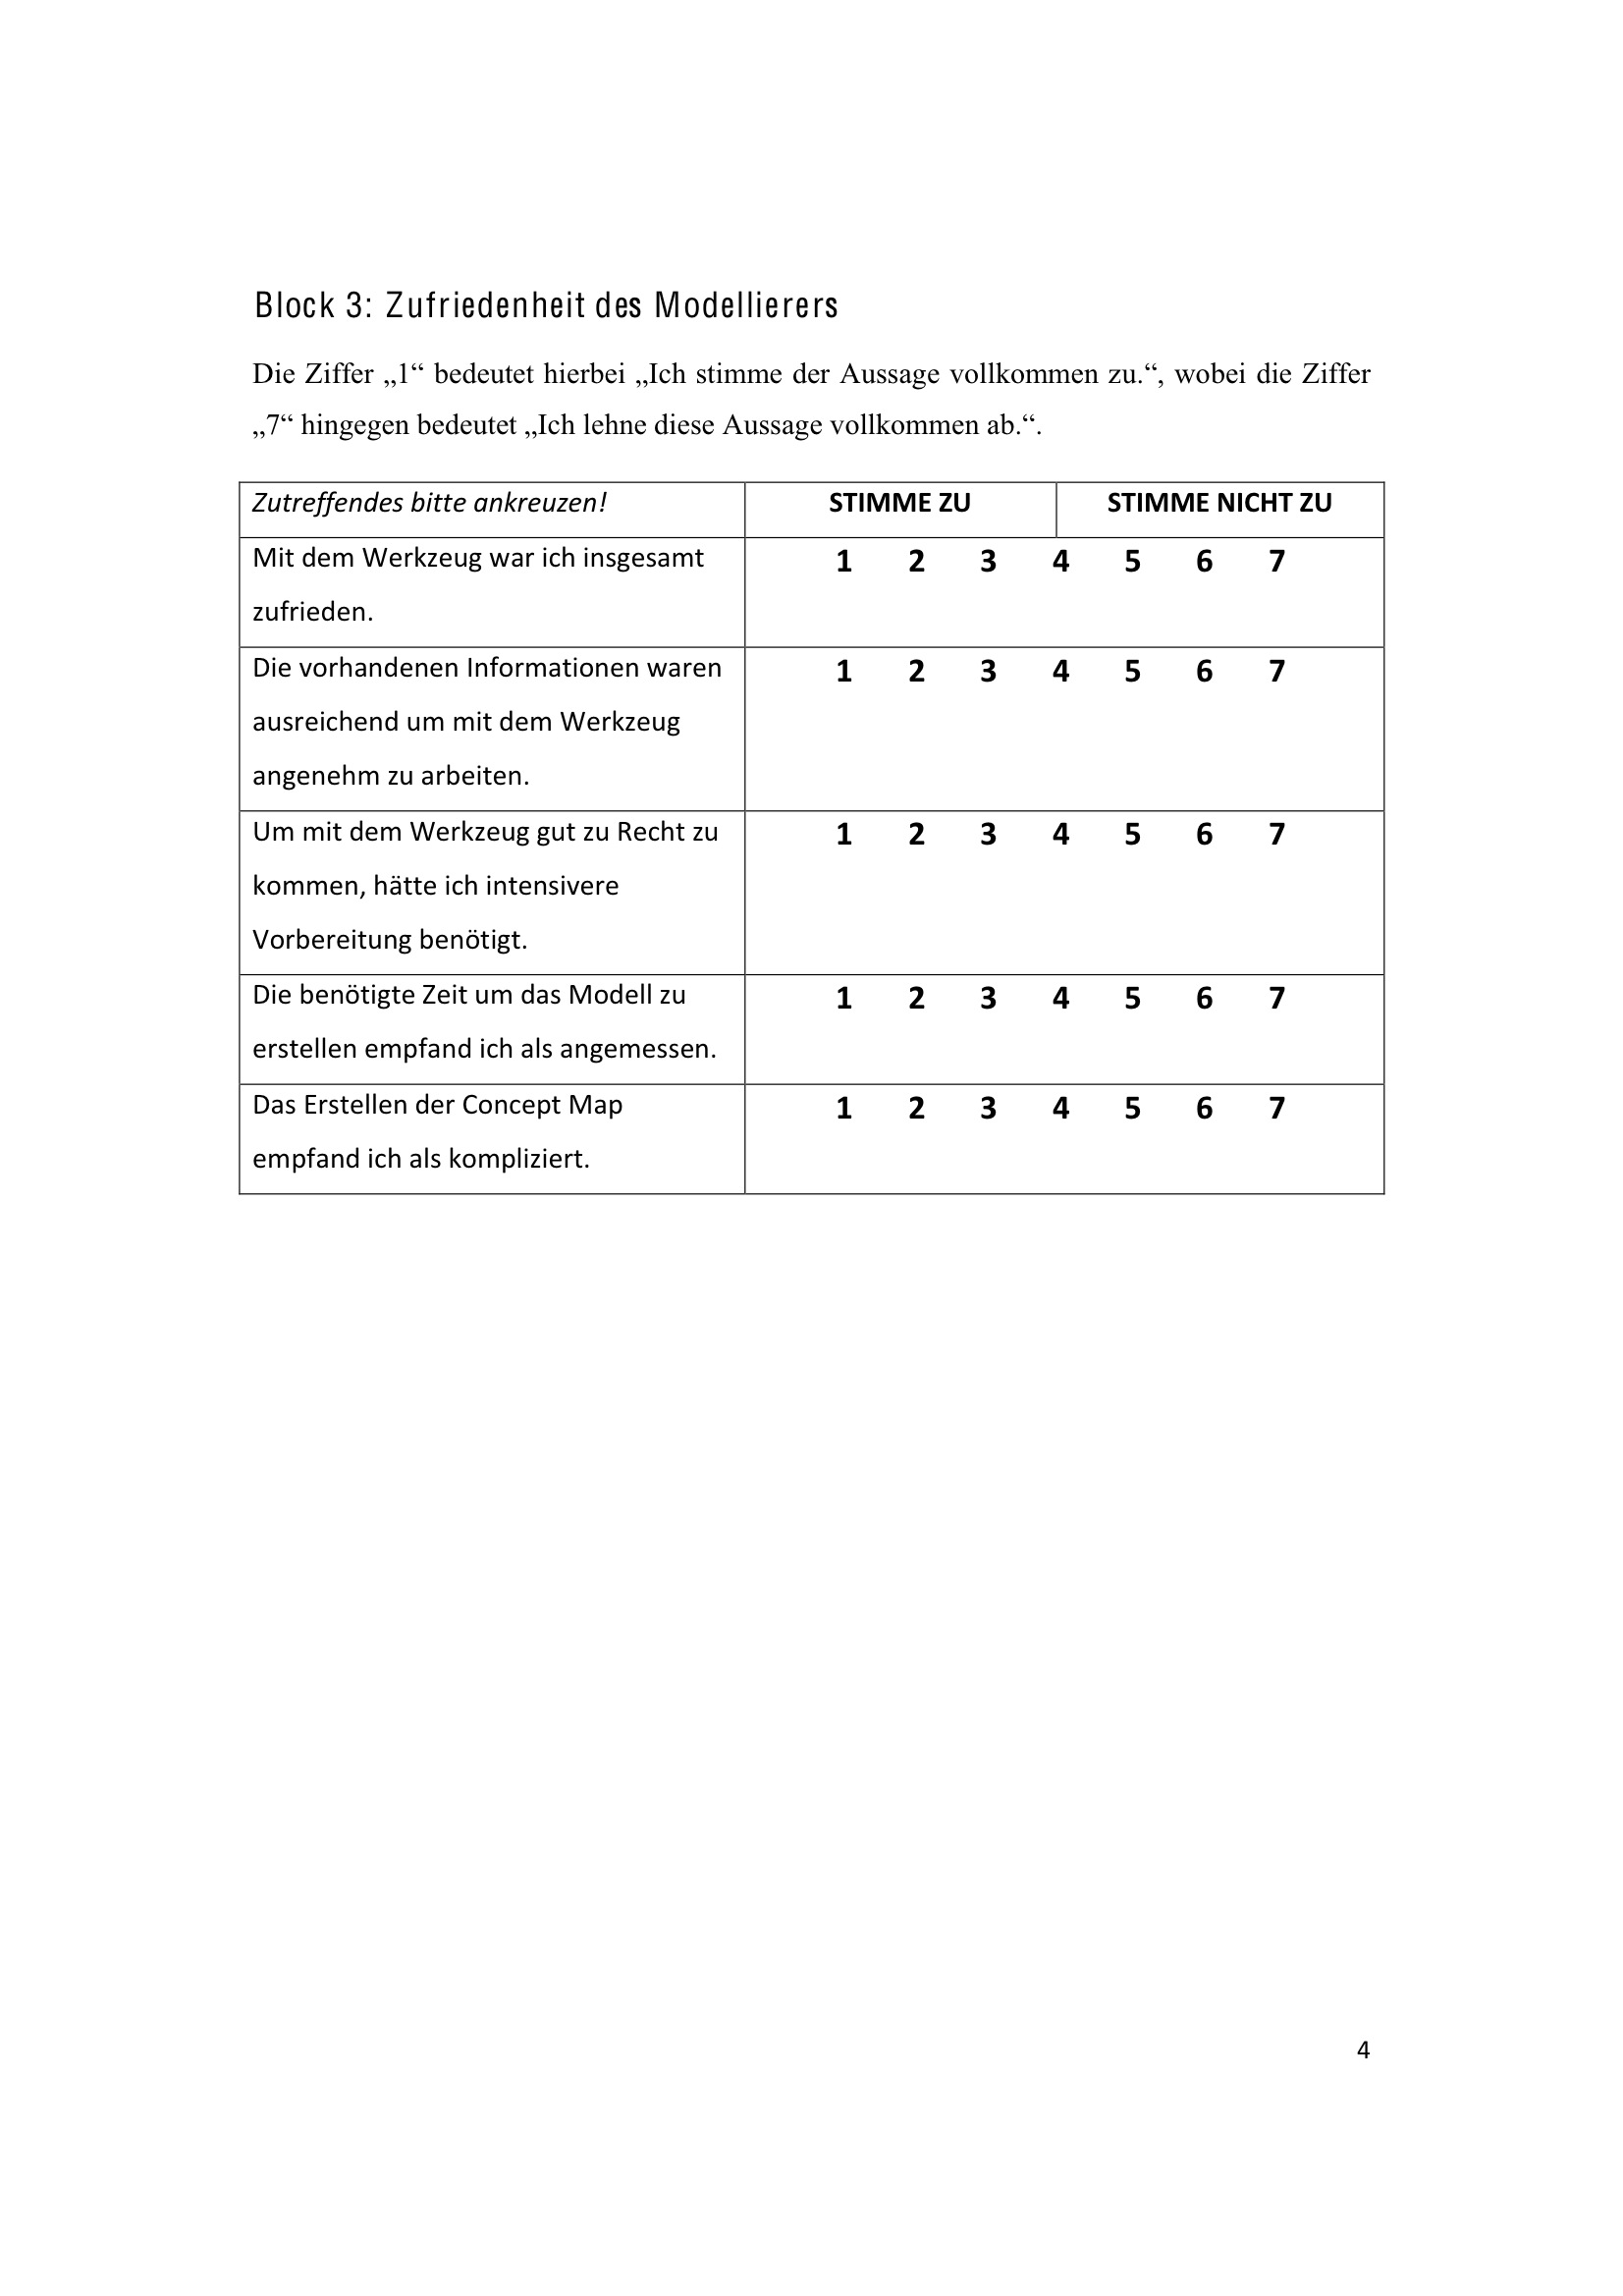
\includegraphics[width=0.9\textwidth]{img/AnhangEmpirie/fb5-04.jpeg}%
	}
	\caption{Fragebogen für Evaluierungsblock 5 - Seite 4}
	\label{fig:img_AnhangEmpirie_fb5-04}
\end{figure}

\begin{figure}[htbp]
	\centering
	\fbox{%
		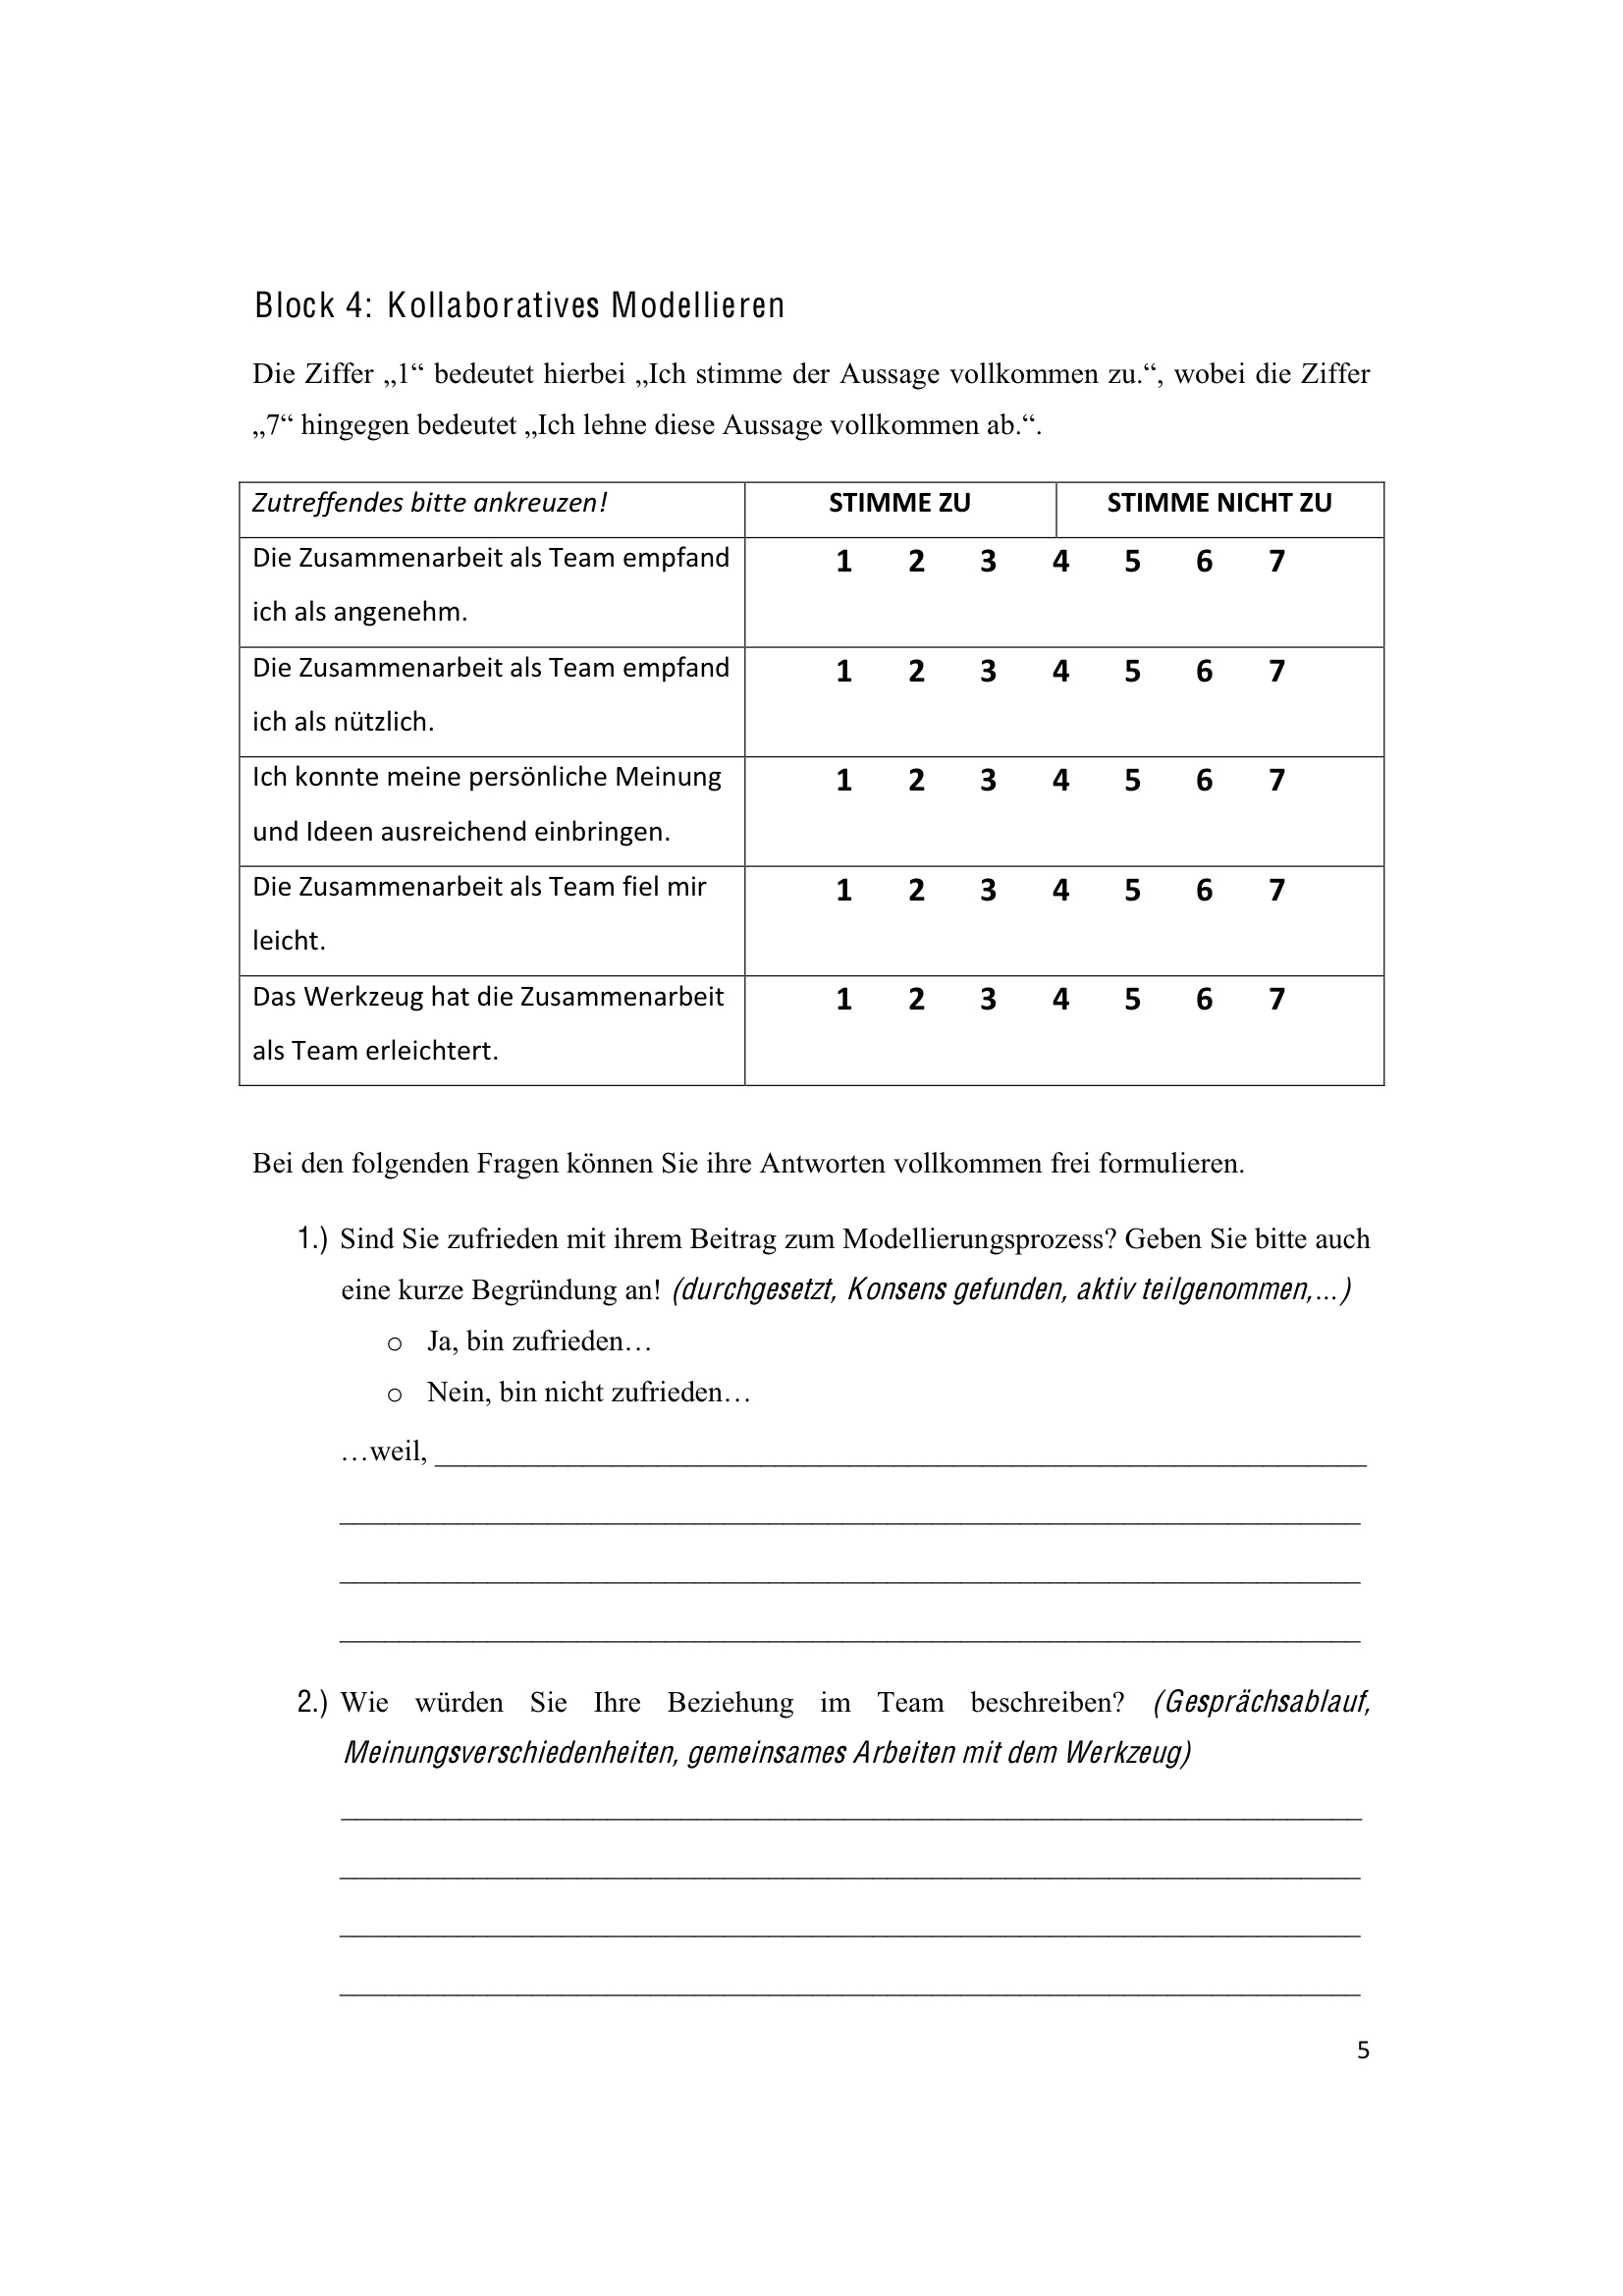
\includegraphics[width=0.9\textwidth]{img/AnhangEmpirie/fb5-05.jpeg}%
	}
	\caption{Fragebogen für Evaluierungsblock 5 - Seite 5}
	\label{fig:img_AnhangEmpirie_fb5-05}
\end{figure}


% section frageboegen (end)

% chapter daten_der_empirischen_untersuchung (end)

\backmatter

\part*{Verzeichnisse}
\addcontentsline{toc}{part}{Verzeichnisse}

\addcontentsline{toc}{chapter}{Abbildungsverzeichnis}
\listoffigures

\newpage
\pagestyle{empty}
\textcolor{white}
.
\textcolor{black}
\newpage
\pagestyle{scrheadings}

\cleardoublepage

\addcontentsline{toc}{chapter}{Tabellenverzeichnis}
\listoftables

\newpage
\pagestyle{empty}
\textcolor{white}
.
\textcolor{black}
\newpage
\pagestyle{scrheadings}

\cleardoublepage

%\addcontentsline{toc}{chapter}{Stichwortverzeichnis}
%\printindex

\addcontentsline{toc}{chapter}{Abkürzungsverzeichnis}
\deftranslation[to=German]{Acronyms}{Abkürzungsverzeichnis}
\printglossary[type=\acronymtype,style=long]

\newpage
\pagestyle{empty}
\textcolor{white}
.
\textcolor{black}
\newpage
\pagestyle{scrheadings}

\cleardoublepage

\manualmark

\addcontentsline{toc}{chapter}{Bildquellen}
\markboth{Abbildungsquellen}{Abbildungsquellen}
\chapter*{Abbildungsquellen}

Dieser Anhang enthält Quellenangaben für alle in dieser Arbeit verwendeten Abbildungen, sofern sie nicht vom Autor erstellt wurden. Sofern nicht anders angegeben, sind alle Abbildungen und Fotos Werke des Autors und dürfen nicht ohne ausdrückliche Zustimmung verwendet werden.

\begin{description}
 \item[Abbildung \ref{fig:img_ArticulationWork_schmidt96-articulation-categories}] Tabelle über abzustimmende Arbeitsaspekte übernommen von \citep{Schmidt96}
 \item[Abbildung \ref{fig:img_ArticulationWork_divitini00_caw}] Abbildung über Zusammenhänge zwischen Arbeitsaspekte übernommen von \citep{Divitini00}
 \item[Abbildung \ref{fig:img_ArticulationWork_mi91-awprocess}] Abbildung des Artikulations-Prozesses nach \citep{Mi91} übernommen von ebenda
 \item[Abbildung \ref{fig:img_MentaleModelle_herrmann_levels_of_structure}] Abbildung über Mentale Modelle im Kontext der Arbeitsmodellierung übernommen von \citep{Herrmann02}
 \item[Abbildung \ref{fig:img_MentaleModelle_iffenthaler_assimilation_akkommodation}] Abbildung über den Zusammenhang zwischen Schemata und Mentalen Modellen übernommen von \citep{Ifenthaler06}
 \item[Abbildung \ref{fig:img_MentaleModelle_iffenthaler_externalisierung}] Abbildung über die Externalisierung mentaler Modelle übernommen von \citep{Ifenthaler06}
 \item[Abbildung \ref{fig:img_MentaleModelle_novak_concept_maps}] Abbildung über die Struktur einer Concept Map übernommen von \citep{Novak06}
 \item[Abbildung \ref{fig:img_ImplementierungUeberblick_marshall_tui_learning}] Taxonomie von Tangible Interfaces im Kontext von Lernprozessen übernommen von \citep{Marshall07}
 \item[Abbildung \ref{fig:img_ImplementierungUeberblick_MCRpd}] Abbildung des MVC- und MCRpd-Modells übernommen von \citep{Ullmer00}
 \item[Abbildung \ref{fig:img_ImplementierungUeberblick_is_tac_ca} ] Abbildung unterschiedlicher Arten von Tangible User Interfaces übernommen von \citep{Ullmer05}
 \item[Abbildung \ref{fig:img_ImplementierungUeberblick_MCRit}] Abbildung des MCRit-Modells übernommen von \citep{Ishii08}
 \item[Abbildung \ref{fig:img_ImplementierungInput_artoolkit}] Bild des AR Toolkit Markers entnommen von www.hitl.washington.edu/ artoolkit/ (Website der Entwickler)
 \item[Abbildung \ref{fig:img_ImplementierungInput_visualcodes}] Bild des Visual Code Markers übernommen von \citep{Rohs04}
 \item[Abbildung \ref{fig:img_Persistenz_SubjectVsOccurrence}] Foto der Tasse lizenzfrei unter http://www.oldskoolman.de/bilder/\\freigestellte-bilder/essen-trinken/kaffee-tasse-freigestellt/, übrige Abbildung eigene Darstellung
 \item[Abbildungen \ref{fig:img_AnhangEmpirie_fb1_1-01} bis \ref{fig:img_AnhangEmpirie_fb5-07}] Abbildungen der verwendeten Fragebögen übernommen von \citep{Bohninger10}, \citep{Wahlmuller10} und \citep{Bindreiter10}
\end{description}


\newpage
\pagestyle{empty}
\textcolor{white}
.
\textcolor{black}
\newpage
\pagestyle{scrheadings}


\addcontentsline{toc}{chapter}{Publikationen im Kontext dieser Arbeit}
\markboth{Publikationen im Kontext dieser Arbeit}{Publikationen im Kontext dieser Arbeit}
\chapter*{Publikationen im Kontext dieser Arbeit}

\begin{description}
	\item[\citet{Oppl05a}] description
	\item[\citet{Oppl06}] description
	\item[\citet{Oppl06a}] description 
	\item[\citet{Oppl07b}] description
	\item[\citet{Oppl07}] description
	\item[\citet{Oppl07a}] description
	\item[\citet{Furtmuller07a}] description
	\item[\citet{Oppl08}] description
	\item[\citet{Oppl08a}] description
	\item[\citet{Oppl09}] description
	\item[\citet{Oppl09b}] description
	\item[\citet{Oppl09c}] description
	\item[\citet{Oppl09d}] description
\end{description}


\automark[section]{chapter} 

\bibliography{Archiv}

\newpage
\pagestyle{empty}
\textcolor{white}
.
\textcolor{black}
\newpage
\cleardoublepage

\addcontentsline{toc}{chapter}{Lebenslauf}
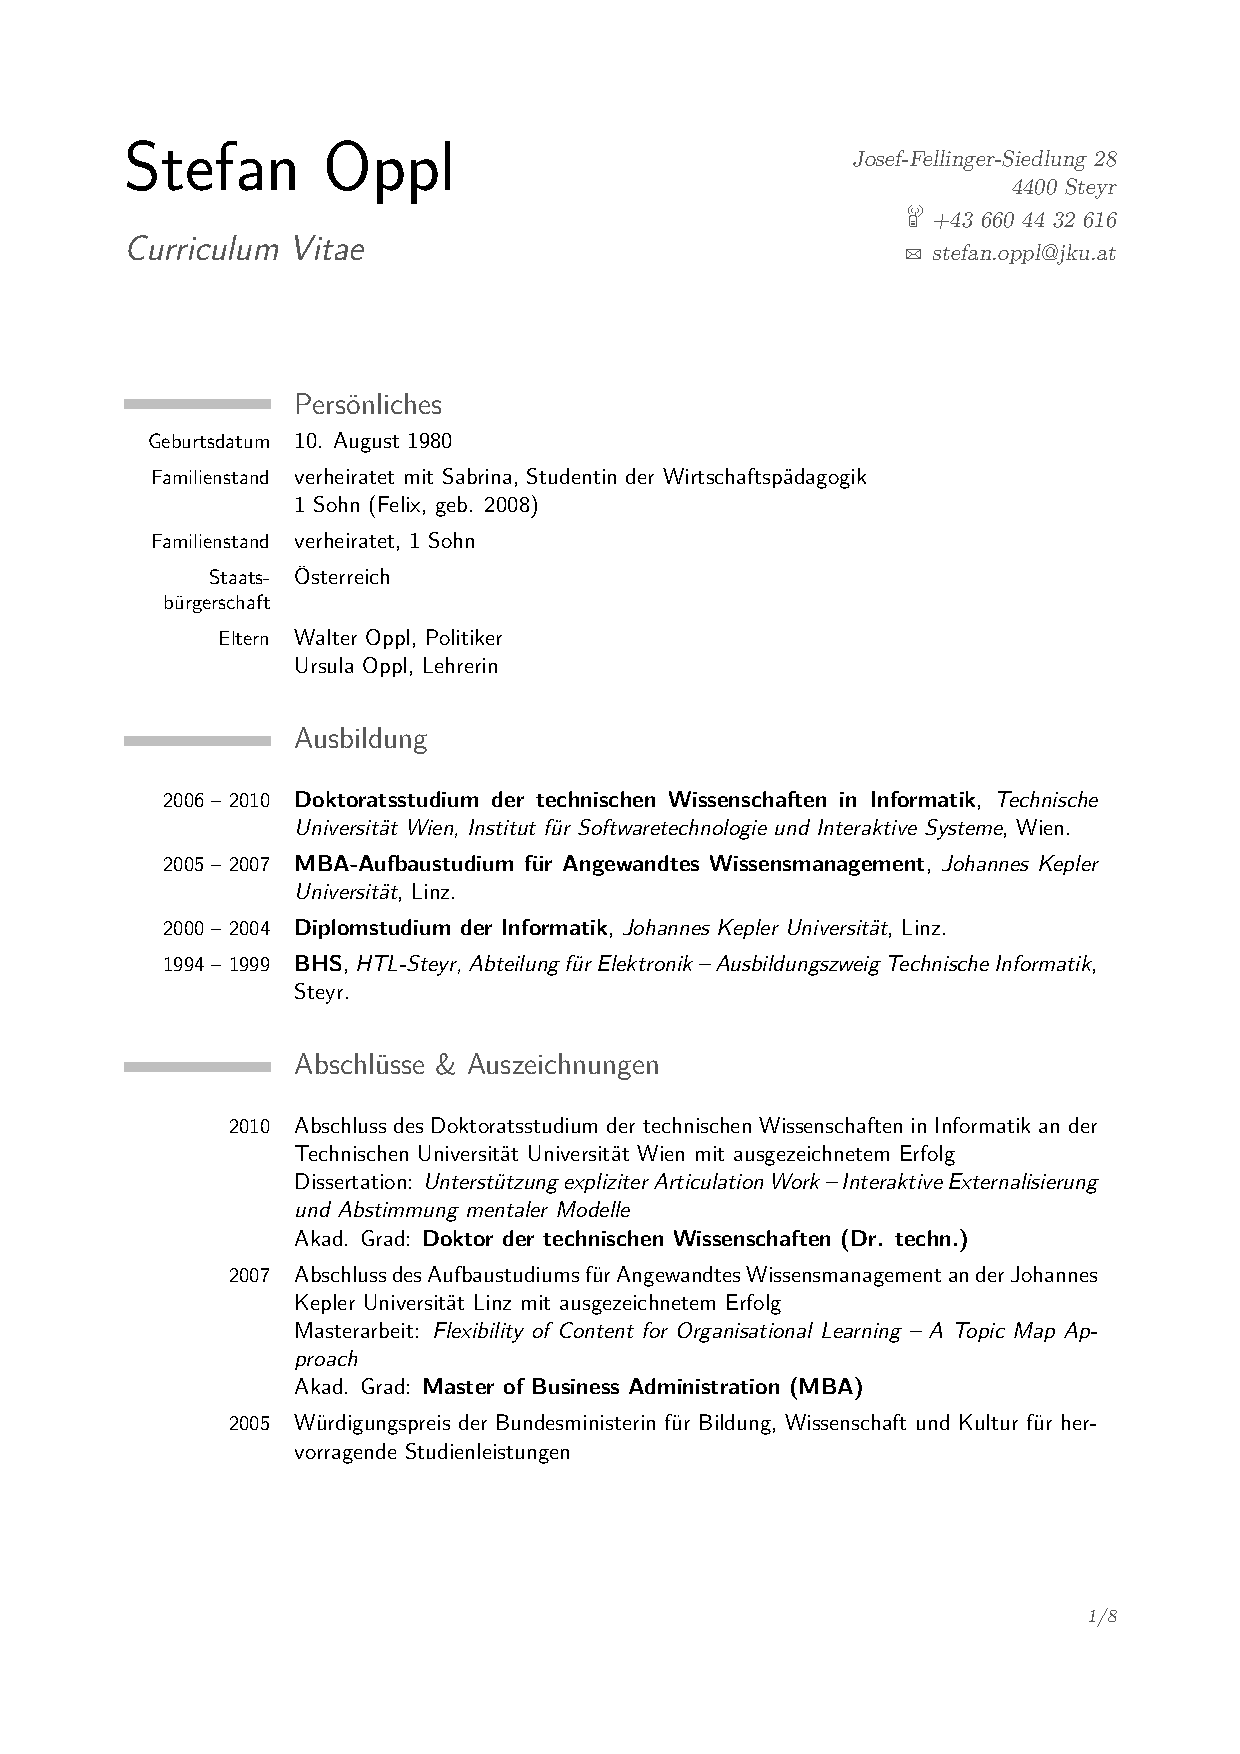
\includepdf[pages=-]{cv}

\newpage
\pagestyle{empty}
\textcolor{white}
.
\textcolor{black}
\newpage
\cleardoublepage

\newpage
\cleardoublepage

\vspace*{\fill}

\begin{center}
Der eine fragt: Was kommt danach? \\
Der andre fragt nur: Ist es recht? \\
Und also unterscheidet sich \\
der Freie von dem Knecht.
\end{center}

\begin{flushright}
Theodor Storm
\end{flushright}

\vspace*{\fill}



\end{document}